\documentclass[11pt]{report}
\usepackage[utf8]{inputenc}
\usepackage[margin=1in]{geometry}
\usepackage{amsmath, amssymb, amsthm}
\usepackage{enumitem}
\usepackage{hyperref}
\usepackage{xcolor}
\usepackage{tcolorbox}
\usepackage{titlesec}
\usepackage{tikz}
\usepackage{pgfplots}
\pgfplotsset{compat=1.18}
\usetikzlibrary{arrows.meta, decorations.markings, calc}
\usepackage{graphicx}
\definecolor{figB}{RGB}{31,90,166}
\definecolor{figR}{RGB}{176,48,48}
\definecolor{figG}{RGB}{34,120,60}
\pgfplotsset{nfig/.style={axis lines=left, axis line style={-stealth, thin},
  tick style={thin}, ticklabel style={font=\scriptsize}, label style={font=\small},
  every axis plot/.append style={line width=0.9pt}, width=0.52\textwidth, height=0.36\textwidth}}
\newcommand{\figcap}[1]{\\[1.5mm]\parbox{0.92\textwidth}{\small\itshape #1}}

% Keep section numbering continuous across chapters (§1, §2, ... not 1.1, 1.2, ...)
\makeatletter
\@removefromreset{section}{chapter}
\makeatother
\renewcommand{\thesection}{\S\arabic{section}}
\renewcommand{\thesubsection}{\arabic{section}.\arabic{subsection}}

% ============================================================================
% AXLER-STYLE COLOR SCHEME
% ============================================================================
% Blue for theorems/propositions/lemmas/corollaries (results to prove)
\definecolor{axlerblue}{RGB}{200, 220, 240}
\definecolor{axlerblueborder}{RGB}{100, 140, 180}

% Yellow/cream for definitions (things to memorize)
\definecolor{axleryellow}{RGB}{255, 250, 205}
\definecolor{axleryellowborder}{RGB}{200, 180, 100}

% Green for examples
\definecolor{axlergreen}{RGB}{220, 245, 220}
\definecolor{axlergreenborder}{RGB}{100, 160, 100}

% Gray for notes/notation
\definecolor{axlergray}{RGB}{245, 245, 245}
\definecolor{axlergrayborder}{RGB}{180, 180, 180}

% Purple for remarks
\definecolor{axlerpurple}{RGB}{235, 225, 245}
\definecolor{axlerpurpleborder}{RGB}{140, 100, 170}

\hypersetup{
    colorlinks=true,
    linkcolor=black,
    urlcolor=axlerblueborder,
    pdfborder={0 0 0}
}

% ============================================================================
% AXLER-STYLE THEOREM BOXES
% ============================================================================
\tcbuselibrary{theorems, skins, breakable}

% Separate counters for each environment type
\newcounter{defcounter}[section]
\renewcommand{\thedefcounter}{\arabic{section}.\arabic{defcounter}}

\newcounter{thmcounter}[section]
\renewcommand{\thethmcounter}{\arabic{section}.\arabic{thmcounter}}

\newcounter{excounter}[section]
\renewcommand{\theexcounter}{\arabic{section}.\arabic{excounter}}

% Definition box (yellow)
\newtcolorbox[use counter=defcounter]{definition}[1][]{
    enhanced,
    colback=axleryellow,
    colframe=axleryellowborder,
    boxrule=0.5pt,
    arc=2pt,
    left=8pt, right=8pt, top=6pt, bottom=6pt,
    fonttitle=\bfseries,
    title={Definition \thedefcounter\ifx\\#1\\\else: #1\fi},
    breakable
}

% Theorem box (blue)
\newtcolorbox[use counter=thmcounter]{theorem}[1][]{
    enhanced,
    colback=axlerblue,
    colframe=axlerblueborder,
    boxrule=0.5pt,
    arc=2pt,
    left=8pt, right=8pt, top=6pt, bottom=6pt,
    fonttitle=\bfseries,
    title={Theorem \thethmcounter\ifx\\#1\\\else\ (#1)\fi},
    breakable
}

% Proposition box (blue, shares theorem counter)
\newtcolorbox[use counter=thmcounter]{proposition}[1][]{
    enhanced,
    colback=axlerblue,
    colframe=axlerblueborder,
    boxrule=0.5pt,
    arc=2pt,
    left=8pt, right=8pt, top=6pt, bottom=6pt,
    fonttitle=\bfseries,
    title={Proposition \thethmcounter\ifx\\#1\\\else\ (#1)\fi},
    breakable
}

% Lemma box (blue, shares theorem counter)
\newtcolorbox[use counter=thmcounter]{lemma}[1][]{
    enhanced,
    colback=axlerblue,
    colframe=axlerblueborder,
    boxrule=0.5pt,
    arc=2pt,
    left=8pt, right=8pt, top=6pt, bottom=6pt,
    fonttitle=\bfseries,
    title={Lemma \thethmcounter\ifx\\#1\\\else\ (#1)\fi},
    breakable
}

% Corollary box (blue, shares theorem counter)
\newtcolorbox[use counter=thmcounter]{corollary}[1][]{
    enhanced,
    colback=axlerblue,
    colframe=axlerblueborder,
    boxrule=0.5pt,
    arc=2pt,
    left=8pt, right=8pt, top=6pt, bottom=6pt,
    fonttitle=\bfseries,
    title={Corollary \thethmcounter\ifx\\#1\\\else\ (#1)\fi},
    breakable
}

% Example box (green)
\newtcolorbox[use counter=excounter]{example}[1][]{
    enhanced,
    colback=axlergreen,
    colframe=axlergreenborder,
    boxrule=0.5pt,
    arc=2pt,
    left=8pt, right=8pt, top=6pt, bottom=6pt,
    fonttitle=\bfseries,
    title={Example \theexcounter\ifx\\#1\\\else: #1\fi},
    breakable
}

% Remark box (purple, unnumbered)
\newtcolorbox{remark}[1][]{
    enhanced,
    colback=axlerpurple,
    colframe=axlerpurpleborder,
    boxrule=0.5pt,
    arc=2pt,
    left=8pt, right=8pt, top=6pt, bottom=6pt,
    fonttitle=\bfseries,
    title={Remark\ifx\\#1\\\else: #1\fi},
    breakable
}

% Note box (gray, unnumbered)
\newtcolorbox{note}[1][]{
    enhanced,
    colback=axlergray,
    colframe=axlergrayborder,
    boxrule=0.5pt,
    arc=2pt,
    left=8pt, right=8pt, top=6pt, bottom=6pt,
    fonttitle=\bfseries,
    title={Note\ifx\\#1\\\else: #1\fi},
    breakable
}

% Notation box (gray, unnumbered)
\newtcolorbox{notation}{
    enhanced,
    colback=axlergray,
    colframe=axlergrayborder,
    boxrule=0.5pt,
    arc=2pt,
    left=8pt, right=8pt, top=6pt, bottom=6pt,
    fonttitle=\bfseries,
    title={Notation},
    breakable
}

% Proof environment (standard, outside boxes)
\renewenvironment{proof}[1][Proof]{\par\noindent\textit{#1.}\ }{\hfill$\square$\par\medskip}

% ============================================================================
% CUSTOM COMMANDS
% ============================================================================
\newcommand{\R}{\mathbb{R}}
\newcommand{\N}{\mathbb{N}}
\newcommand{\Z}{\mathbb{Z}}
\newcommand{\Q}{\mathbb{Q}}
\newcommand{\eps}{\varepsilon}
\newcommand{\parti}[2]{\frac{\partial #1}{\partial #2}}

% ============================================================================
% TITLE FORMATTING
% ============================================================================
\titleformat{\section}{\Large\bfseries}{\thesection}{1em}{}
\titleformat{\subsection}{\large\bfseries}{\thesubsection}{1em}{}

% No indentation throughout
\setlength{\parindent}{0pt}
\setlength{\parskip}{6pt}

% TOC shows sections and subsections, not subsubsections
\setcounter{tocdepth}{2}

\title{\textbf{MATH 452: Multivariable Analysis}\\Lecture Notes}
\author{Prof.\ Tian Jing}
\date{Winter 2026}

\begin{document}
\maketitle

\tableofcontents
\newpage

\section*{Course Information}
\textbf{Office:} EH 4060 \quad \textbf{Office Hours:} Monday 10am

\textbf{Exams:} Midterm I: Fri 2/6 (in class), Midterm II: Fri 3/13 (in class), Final: Thu 4/30, 10:30am--12:30pm. Late drop: 3/30.

\textbf{Grading:} 20\% HW, 20\% Midterm I, 20\% Midterm II, 40\% Final. Can miss at most 1 exam.

\textbf{Textbook:} \textit{Introduction to Calculus and Analysis, Vol.\ II}, available at university library.

\textbf{References:}
\begin{itemize}[nosep]
    \item \textit{Advanced Calculus of Several Variables} --- C.H.\ Edwards
    \item \textit{Principles of Mathematical Analysis} --- Walter Rudin
    \item \textit{Calculus on Manifolds} --- Michael Spivak
\end{itemize}

\textbf{Topics:} Sets, open/closed, notations; partial derivatives, differentiability, MVT; differential operators (gradients, directional derivatives, chain rule); Implicit Function Theorem; surfaces, tangent planes; max/min of multivariable functions, Lagrange multipliers; multi-integrals; change of variable (Jacobian); surface integrals; Green's theorem, Stokes' theorem; differential forms, exterior derivatives.

\hrulefill

\newpage
\part{Differential Calculus in Several Variables}

\chapter{Foundations}

\section{Sequences and Limits in $\R^n$}

\begin{definition}[Convergence of Sequences in $\R^n$]
A sequence $(a_n) \subset \R^n$ \textbf{converges} to $A \in \R^n$ if
\[
\forall\, \eps > 0,\; \exists\, N \in \N,\; \forall\, n \geq N: \quad |a_n - A| < \eps.
\]
For vectors in $\R^2$, the distance is $|(a_n, b_n) - (A, B)| = \sqrt{(a_n - A)^2 + (b_n - B)^2}$.
\end{definition}

\begin{example}
Show that $(e^{-n}\cos(n), e^{-n}\sin(n)) \to (0, 0)$.

\textbf{Scratch work:} Compute the distance:
\[
|(e^{-n}\cos(n), e^{-n}\sin(n)) - (0, 0)| = \sqrt{e^{-2n}\cos^2(n) + e^{-2n}\sin^2(n)} = e^{-n}.
\]
We need $e^{-n} < \eps$, i.e., $n > \ln(1/\eps)$.
\end{example}

\begin{proof}
Let $\eps > 0$. Without loss of generality, assume $\eps < 1$. Let $N = \lfloor \ln(1/\eps) \rfloor + 1$. Then for all $n \geq N$, we have $n > \ln(1/\eps)$, so $e^{-n} < \eps$. Therefore
\[
|(e^{-n}\cos(n), e^{-n}\sin(n)) - (0, 0)| = e^{-n} < \eps. \qedhere
\]
\end{proof}

\section{Open and Closed Sets}

\begin{definition}[Open Ball]
The \textbf{open ball} (spherical neighborhood) centered at $x \in \R^n$ with radius $r > 0$ is
\[
B(x, r) := \{y \in \R^n : |y - x| < r\}.
\]
Alternative notations: $B_r(x)$ or simply $B_n$ when the center is understood.
\end{definition}

\begin{definition}[Square Neighborhood]
A \textbf{square neighborhood} centered at $(x_0, y_0) \in \R^2$ with side length $2\delta$ is
\[
\{(x, y) \in \R^2 : |x - x_0| < \delta \text{ and } |y - y_0| < \delta\}.
\]
\end{definition}

\begin{remark}
Open balls and square neighborhoods are topologically equivalent for most purposes.
\end{remark}

\begin{definition}[Interior, Exterior, and Boundary Points]
Let $E \subseteq \R^n$ and $x \in \R^n$.
\begin{itemize}[itemsep=4pt]
    \item $x$ is an \textbf{interior point} of $E$ if $\exists\, \eps > 0$ such that $B(x, \eps) \subseteq E$.
    \item $x$ is an \textbf{exterior point} of $E$ if $\exists\, \eps > 0$ such that $B(x, \eps) \subseteq E^c$.
    \item $x$ is a \textbf{boundary point} of $E$ if for all $\eps > 0$: $B(x, \eps) \cap E \neq \emptyset$ and $B(x, \eps) \cap E^c \neq \emptyset$.
\end{itemize}
\end{definition}

\begin{center}
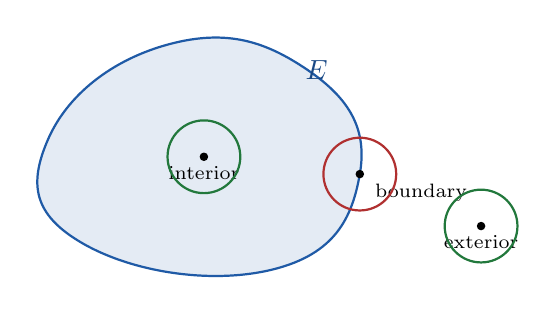
\begin{tikzpicture}[scale=1.1]
% the set E: a blob
\draw[thick, figB, fill=figB!12] plot[smooth cycle, tension=0.8] coordinates {(0,0) (2.2,-0.3) (3.2,0.8) (2.6,2.0) (1.0,2.3) (-0.4,1.2)};
\node[figB!80!black] at (2.7,2.0) {$E$};
% interior point
\filldraw (1.4,1.0) circle (1.2pt) node[below, font=\scriptsize] {interior};
\draw[figG, thick] (1.4,1.0) circle (0.42);
% boundary point (exactly on the curve: a control point of the cycle)
\filldraw (3.2,0.8) circle (1.2pt) node[below right, font=\scriptsize, xshift=2pt] {boundary};
\draw[figR, thick] (3.2,0.8) circle (0.42);
% exterior point
\filldraw (4.6,0.2) circle (1.2pt) node[below, font=\scriptsize] {exterior};
\draw[figG, thick] (4.6,0.2) circle (0.42);
\end{tikzpicture}%
\figcap{An interior point has a ball entirely inside $E$; an exterior point has a ball entirely outside; a boundary point's every ball meets both $E$ and $E^c$.}
\end{center}

\begin{example}
For $E = [0, 1)$, the points $0$ and $1$ are both boundary points.
\end{example}

\begin{definition}[Open and Closed Sets]
Let $E \subseteq \R^n$.
\begin{itemize}[itemsep=4pt]
    \item $E$ is \textbf{open} if every point of $E$ is an interior point.
    \item $E$ is \textbf{closed} if $E$ contains all its boundary points.
\end{itemize}
\end{definition}

\begin{notation}
$\partial E$ denotes the set of boundary points of $E$.
\end{notation}

\begin{definition}[Closure]
The \textbf{closure} of $E$ is $\overline{E} := E \cup \partial E$, the smallest closed set containing $E$.
\end{definition}

\section{Continuity and Limits of Functions}

\begin{definition}[Continuity]
A function $f : \R^2 \to \R$ is \textbf{continuous} at $(x_0, y_0)$ if
\[
\forall\, \eps > 0,\; \exists\, \delta > 0,\; \forall\, (x, y) \in \R^2: \quad |(x, y) - (x_0, y_0)| < \delta \implies |f(x, y) - f(x_0, y_0)| < \eps.
\]
\end{definition}

\begin{center}
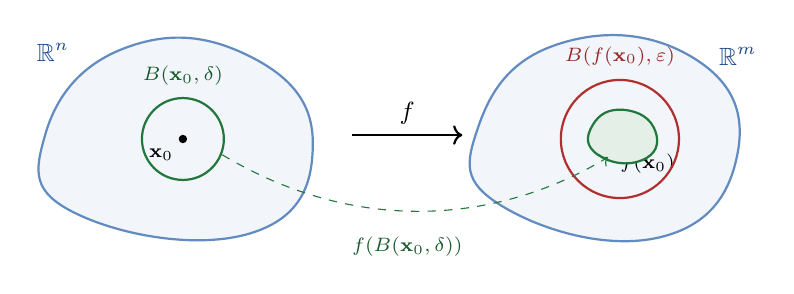
\begin{tikzpicture}[scale=1.0]
% domain side
\draw[thick, figB!70, fill=figB!6] plot[smooth cycle, tension=0.8] coordinates {(0,0) (2.2,-0.25) (3.0,0.9) (2.2,2.0) (0.6,2.1) (-0.4,1.0)};
\node[figB!80!black, font=\small] at (-0.3,2.05) {$\R^n$};
\coordinate (P) at (1.35,0.95);
\filldraw (P) circle (1.3pt) node[below left, font=\scriptsize] {$\mathbf{x}_0$};
\draw[figG, thick] (P) circle (0.52);
\node[figG!75!black, font=\scriptsize] at (1.35,1.75) {$B(\mathbf{x}_0,\delta)$};
% map arrow
\draw[->, thick] (3.5,1.0) -- (4.9,1.0) node[midway, above, font=\small] {$f$};
% codomain side
\begin{scope}[shift={(5.4,0)}]
\draw[thick, figB!70, fill=figB!6] plot[smooth cycle, tension=0.8] coordinates {(0,0.1) (2.0,-0.3) (3.0,0.8) (2.4,2.0) (0.7,2.15) (-0.3,1.1)};
\node[figB!80!black, font=\small] at (3.0,2.0) {$\R^m$};
\coordinate (Q) at (1.5,0.95);
\filldraw (Q) circle (1.3pt) node[font=\scriptsize, yshift=-9pt, xshift=10pt] {$f(\mathbf{x}_0)$};
\draw[figR, thick] (Q) circle (0.75);
\node[figR!85!black, font=\scriptsize] at (1.5,2.0) {$B(f(\mathbf{x}_0),\varepsilon)$};
% image blob of the delta ball, inside epsilon ball
\draw[figG, thick, fill=figG!12] plot[smooth cycle, tension=0.9] coordinates {(1.22,0.75) (1.78,0.68) (1.95,1.05) (1.55,1.32) (1.15,1.12)};
\end{scope}
% dashed image arrow
\draw[->, dashed, figG] (1.85,0.75) .. controls (3.6,-0.3) and (5.4,-0.1) .. (6.75,0.72);
\node[figG!75!black, font=\scriptsize] at (4.2,-0.42) {$f(B(\mathbf{x}_0,\delta))$};
\end{tikzpicture}%
\figcap{Continuity at $\mathbf{x}_0$ as a mapping statement: for every target tolerance $\varepsilon$ (red ball), there is an input tolerance $\delta$ (green ball) whose entire image lands inside the red ball. The green image blob need not be a ball --- it only needs to be trapped.}
\end{center}


\begin{example}[Discontinuity via Path Dependence]
Consider
\[
f(x, y) = \begin{cases} \dfrac{2xy}{x^2 + y} & (x, y) \neq (0,0) \\[6pt] 0 & (x, y) = (0, 0). \end{cases}
\]

\textbf{Claim:} $f$ is not continuous at $(0, 0)$.

\textbf{Along $x$-axis} ($y = 0$, $x \neq 0$): $|f(x, 0) - f(0, 0)| = 0 < \eps$. Same for $y$-axis.

\textbf{Along $y = x$:} $|f(x, x) - f(0, 0)| = \left|\dfrac{2x^2}{2x^2}\right| = 1$.

Choose $\eps = \tfrac{1}{2}$. No $\delta > 0$ works, so $f$ is not continuous at $(0, 0)$.
\end{example}

\subsection{Algebra of Continuous Functions}

The following theorems show that continuous functions are closed under the standard algebraic operations.

\begin{theorem}[Sum and Difference of Continuous Functions]
If $f, g : \R^2 \to \R$ are continuous at $(x_0, y_0)$, then $f + g$ and $f - g$ are continuous at $(x_0, y_0)$.
\end{theorem}

\begin{proof}
We prove continuity of $f + g$; the proof for $f - g$ is similar.

Let $\varepsilon > 0$. We need to find $\delta > 0$ such that
\[
|(x, y) - (x_0, y_0)| < \delta \implies |(f + g)(x, y) - (f + g)(x_0, y_0)| < \varepsilon.
\]

Since $f$ is continuous at $(x_0, y_0)$, there exists $\delta_1 > 0$ such that
\[
|(x, y) - (x_0, y_0)| < \delta_1 \implies |f(x, y) - f(x_0, y_0)| < \frac{\varepsilon}{2}.
\]

Since $g$ is continuous at $(x_0, y_0)$, there exists $\delta_2 > 0$ such that
\[
|(x, y) - (x_0, y_0)| < \delta_2 \implies |g(x, y) - g(x_0, y_0)| < \frac{\varepsilon}{2}.
\]

Let $\delta = \min\{\delta_1, \delta_2\}$. Then for $|(x, y) - (x_0, y_0)| < \delta$:
\begin{align*}
|(f + g)(x, y) - (f + g)(x_0, y_0)| &= |f(x, y) - f(x_0, y_0) + g(x, y) - g(x_0, y_0)| \\
&\leq |f(x, y) - f(x_0, y_0)| + |g(x, y) - g(x_0, y_0)| \\
&< \frac{\varepsilon}{2} + \frac{\varepsilon}{2} = \varepsilon.
\end{align*}
Hence $f + g$ is continuous at $(x_0, y_0)$.
\end{proof}

\begin{theorem}[Product of Continuous Functions]
If $f, g : \R^2 \to \R$ are continuous at $(x_0, y_0)$, then $f \cdot g$ is continuous at $(x_0, y_0)$.
\end{theorem}

\begin{proof}
Let $\varepsilon > 0$. We use the identity:
\[
f(x,y) g(x,y) - f(x_0, y_0) g(x_0, y_0) = f(x,y)[g(x,y) - g(x_0, y_0)] + g(x_0, y_0)[f(x,y) - f(x_0, y_0)].
\]

Since $f$ is continuous at $(x_0, y_0)$, it is bounded near $(x_0, y_0)$: there exist $\delta_1 > 0$ and $M > 0$ such that
\[
|(x, y) - (x_0, y_0)| < \delta_1 \implies |f(x, y)| \leq M.
\]
(We can take $M = |f(x_0, y_0)| + 1$ by choosing $\delta_1$ small enough.)

Let $K = |g(x_0, y_0)|$. Choose $\delta_2 > 0$ such that
\[
|(x, y) - (x_0, y_0)| < \delta_2 \implies |g(x, y) - g(x_0, y_0)| < \frac{\varepsilon}{2M}.
\]

Choose $\delta_3 > 0$ such that
\[
|(x, y) - (x_0, y_0)| < \delta_3 \implies |f(x, y) - f(x_0, y_0)| < \frac{\varepsilon}{2(K + 1)}.
\]

Let $\delta = \min\{\delta_1, \delta_2, \delta_3\}$. Then for $|(x, y) - (x_0, y_0)| < \delta$:
\begin{align*}
|f(x,y) g(x,y) - f(x_0, y_0) g(x_0, y_0)| &\leq |f(x,y)| \cdot |g(x,y) - g(x_0, y_0)| + |g(x_0, y_0)| \cdot |f(x,y) - f(x_0, y_0)| \\
&< M \cdot \frac{\varepsilon}{2M} + K \cdot \frac{\varepsilon}{2(K + 1)} \\
&< \frac{\varepsilon}{2} + \frac{\varepsilon}{2} = \varepsilon.
\end{align*}
Hence $f \cdot g$ is continuous at $(x_0, y_0)$.
\end{proof}

\begin{theorem}[Quotient of Continuous Functions]
If $f, g : \R^2 \to \R$ are continuous at $(x_0, y_0)$ and $g(x_0, y_0) \neq 0$, then $f/g$ is continuous at $(x_0, y_0)$.
\end{theorem}

\begin{proof}
It suffices to prove that $1/g$ is continuous at $(x_0, y_0)$ (then apply the product rule to $f \cdot (1/g)$).

Let $\varepsilon > 0$ and let $L = g(x_0, y_0) \neq 0$.

\textbf{Step 1:} Since $g$ is continuous and $L \neq 0$, there exists $\delta_1 > 0$ such that
\[
|(x, y) - (x_0, y_0)| < \delta_1 \implies |g(x, y) - L| < \frac{|L|}{2}.
\]
This implies $|g(x, y)| > |L| - \frac{|L|}{2} = \frac{|L|}{2} > 0$, so $g(x,y) \neq 0$ near $(x_0, y_0)$.

\textbf{Step 2:} We have
\[
\left|\frac{1}{g(x,y)} - \frac{1}{L}\right| = \frac{|L - g(x,y)|}{|g(x,y)| \cdot |L|} < \frac{|g(x,y) - L|}{\frac{|L|}{2} \cdot |L|} = \frac{2|g(x,y) - L|}{|L|^2}.
\]

\textbf{Step 3:} Choose $\delta_2 > 0$ such that
\[
|(x, y) - (x_0, y_0)| < \delta_2 \implies |g(x, y) - L| < \frac{\varepsilon |L|^2}{2}.
\]

Let $\delta = \min\{\delta_1, \delta_2\}$. Then for $|(x, y) - (x_0, y_0)| < \delta$:
\[
\left|\frac{1}{g(x,y)} - \frac{1}{L}\right| < \frac{2}{|L|^2} \cdot \frac{\varepsilon |L|^2}{2} = \varepsilon.
\]
Hence $1/g$ is continuous at $(x_0, y_0)$.
\end{proof}

\begin{theorem}[Composition of Continuous Functions]
If $\varphi, \psi : \R^2 \to \R$ are continuous at $(a, b)$, and $f : \R^2 \to \R$ is continuous at $(\varphi(a,b), \psi(a,b))$, then 
\[
g(x,y) = f(\varphi(x,y), \psi(x,y))
\]
is continuous at $(a, b)$.
\end{theorem}

\begin{proof}
Let $\varepsilon > 0$. We need to find $\delta > 0$ such that $|(x,y) - (a,b)| < \delta$ implies $|g(x,y) - g(a,b)| < \varepsilon$.

\textbf{Step 1:} Since $f$ is continuous at $(\varphi(a,b), \psi(a,b))$, there exists $\sigma > 0$ such that
\[
|(\xi, \eta) - (\varphi(a,b), \psi(a,b))| < \sigma \implies |f(\xi, \eta) - f(\varphi(a,b), \psi(a,b))| < \varepsilon.
\]

\textbf{Step 2:} Since $\varphi$ is continuous at $(a,b)$, there exists $\delta_1 > 0$ such that
\[
|(x,y) - (a,b)| < \delta_1 \implies |\varphi(x,y) - \varphi(a,b)| < \frac{\sigma}{\sqrt{2}}.
\]

\textbf{Step 3:} Since $\psi$ is continuous at $(a,b)$, there exists $\delta_2 > 0$ such that
\[
|(x,y) - (a,b)| < \delta_2 \implies |\psi(x,y) - \psi(a,b)| < \frac{\sigma}{\sqrt{2}}.
\]

\textbf{Conclusion:} Let $\delta = \min\{\delta_1, \delta_2\}$. For $|(x,y) - (a,b)| < \delta$:
\[
|(\varphi(x,y), \psi(x,y)) - (\varphi(a,b), \psi(a,b))| = \sqrt{|\varphi(x,y) - \varphi(a,b)|^2 + |\psi(x,y) - \psi(a,b)|^2} < \sqrt{\frac{\sigma^2}{2} + \frac{\sigma^2}{2}} = \sigma.
\]
Hence by Step 1: $|f(\varphi(x,y), \psi(x,y)) - f(\varphi(a,b), \psi(a,b))| < \varepsilon$, i.e., $|g(x,y) - g(a,b)| < \varepsilon$.
\end{proof}

\begin{remark}[Summary: Algebra of Continuous Functions]
If $f$ and $g$ are continuous at $(x_0, y_0)$, then so are:
\begin{center}
\begin{tabular}{|c|c|}
\hline
\textbf{Operation} & \textbf{Condition} \\
\hline
$f + g$ & (none) \\
$f - g$ & (none) \\
$f \cdot g$ & (none) \\
$f / g$ & $g(x_0, y_0) \neq 0$ \\
$h \circ (f, g)$ & $h$ continuous at $(f(x_0, y_0), g(x_0, y_0))$ \\
\hline
\end{tabular}
\end{center}
\end{remark}

\begin{definition}[Limit of a Function]
We write $\displaystyle\lim_{(x,y) \to (x_0, y_0)} f(x, y) = A$ if there exists $A$ such that
\[
\forall\, \eps > 0,\; \exists\, \delta > 0,\; \forall\, (x, y): \quad 0 < |(x, y) - (x_0, y_0)| < \delta \implies |f(x, y) - A| < \eps.
\]
\end{definition}

\begin{example}[Nonexistence of Limit]
Let $f(x, y) = \dfrac{2xy}{x^2 + y^2}$ for $(x, y) \neq (0, 0)$. Then $f$ has no limit at $(0, 0)$.

Along $y = kx$: $f(x, kx) = \dfrac{2kx^2}{x^2 + k^2 x^2} = \dfrac{2k}{1 + k^2}$, which depends on $k$.
\end{example}

\begin{definition}[Big-O and Little-o Notation]
Let $\rho = \sqrt{x^2 + y^2}$.
\begin{itemize}[itemsep=4pt]
    \item $f(x, y) = O(\rho)$ means $|f(x, y)| \leq C\rho$ for some constant $C$ near the origin.
    \item $f(x, y) = o(\rho)$ means $\displaystyle\lim_{\rho \to 0} \frac{f(x, y)}{\rho} = 0$ (i.e., $f$ vanishes faster than $\rho$).
\end{itemize}
\end{definition}

\begin{example}
$f(x, y) = x^2 + y^2 = o(\rho)$, since $\dfrac{x^2 + y^2}{\sqrt{x^2 + y^2}} = \sqrt{x^2 + y^2} \to 0$.
\end{example}

\chapter{Differentiation}

\section{Partial Derivatives}

\begin{definition}[Partial Derivatives]
For $f : \R^2 \to \R$ defined near $(x, y)$:
\[
f_x(x, y) = \parti{f}{x} = \lim_{h \to 0} \frac{f(x + h, y) - f(x, y)}{h}, \qquad f_y(x, y) = \parti{f}{y} = \lim_{k \to 0} \frac{f(x, y + k) - f(x, y)}{k}.
\]
\end{definition}

\begin{center}
\includegraphics[width=0.66\textwidth]{pyfigs/f13_partials.pdf}%
\figcap{Partial derivatives are ordinary derivatives of slice curves: cutting the surface along $y = y_0$ gives a single-variable function of $x$ whose slope at the point is $f_x$; cutting along $x = x_0$ gives the $f_y$ slice. Each partial sees only its own slice --- this is why the existence of both partials is far weaker than differentiability (\S6).}
\end{center}


\begin{example}[Partials Exist but Function Discontinuous]
Let $f(x, y) = \dfrac{2xy}{x^2 + y^2}$ for $(x,y) \neq (0,0)$ and $f(0,0) = 0$. Then
\[
f_x(0, 0) = \lim_{h \to 0} \frac{f(h, 0) - f(0, 0)}{h} = 0, \qquad f_y(0, 0) = 0.
\]
So partial derivatives exist at $(0, 0)$, but $f$ is not continuous there.
\end{example}

\begin{theorem}[Bounded Partials Imply Continuity]
Let $R$ be an open rectangle. If $f_x$ and $f_y$ both exist on $R$ and are bounded (i.e., $|f_x|, |f_y| \leq M$ for some $M > 0$), then $f$ is continuous on $R$.
\end{theorem}

\begin{proof}
Let $(x_0, y_0) \in R$ and let $\eps > 0$. Since $R$ is open, there exists $r > 0$ such that $B((x_0, y_0), r) \subseteq R$.

For $(h, k)$ with $|(h, k)| < r$, the points $(x_0, y_0)$, $(x_0 + h, y_0)$, and $(x_0 + h, y_0 + k)$ all lie in $R$. By the triangle inequality:
\[
|f(x_0 + h, y_0 + k) - f(x_0, y_0)| \leq |f(x_0 + h, y_0 + k) - f(x_0 + h, y_0)| + |f(x_0 + h, y_0) - f(x_0, y_0)|.
\]

\textbf{Second term:} Define $g(x) = f(x, y_0)$ for $x \in [x_0, x_0 + h]$ (or $[x_0 + h, x_0]$ if $h < 0$). Since $f_x$ exists on $R$, the function $g$ is differentiable with $g'(x) = f_x(x, y_0)$. By the Mean Value Theorem, there exists $\theta(h) \in [0, 1]$ such that
\[
g(x_0 + h) - g(x_0) = h \cdot g'(x_0 + \theta(h) \cdot h) = h \cdot f_x(x_0 + \theta(h) \cdot h, y_0).
\]
Since $|f_x| \leq M$, we have $|f(x_0 + h, y_0) - f(x_0, y_0)| \leq M|h|$.

\textbf{First term:} Define $\psi(y) = f(x_0 + h, y)$ for $y \in [y_0, y_0 + k]$. By MVT, there exists $\eta(h, k) \in [0, 1]$ such that
\[
\psi(y_0 + k) - \psi(y_0) = k \cdot \psi'(y_0 + \eta(h,k) \cdot k) = k \cdot f_y(x_0 + h, y_0 + \eta(h,k) \cdot k).
\]
Since $|f_y| \leq M$, we have $|f(x_0 + h, y_0 + k) - f(x_0 + h, y_0)| \leq M|k|$.

(Note: $\theta$ depends on $h$; $\eta$ depends on $h$ and $k$. But the bounds $M|h|$ and $M|k|$ are uniform.)

\textbf{Combining:} 
\[
|f(x_0 + h, y_0 + k) - f(x_0, y_0)| \leq M|h| + M|k| \leq 2M\sqrt{h^2 + k^2}.
\]

Let $\delta = \min\left(r, \dfrac{\eps}{2M}\right)$. Then for $|(h, k)| < \delta$:
\[
|f(x_0 + h, y_0 + k) - f(x_0, y_0)| \leq 2M \cdot \delta \leq \eps.
\]
Hence $f$ is continuous at $(x_0, y_0)$.
\end{proof}

\begin{example}[Second Partials of $r = \sqrt{x^2 + y^2}$]
\[
r_x = \frac{x}{r}, \quad r_y = \frac{y}{r}, \quad r_{xx} = \frac{r^2 - x^2}{r^3}, \quad r_{yy} = \frac{r^2 - y^2}{r^3}, \quad r_{xy} = r_{yx} = -\frac{xy}{r^3}.
\]
Note: $\Delta r = r_{xx} + r_{yy} = \dfrac{1}{r}$.
\end{example}

\section{Equality of Mixed Partials}

\begin{theorem}[Schwarz--Clairaut]
Let $R$ be an open rectangle. If $f_{xy}$ and $f_{yx}$ exist and are continuous on $R$, then $f_{xy} = f_{yx}$ on $R$.
\end{theorem}

\begin{center}
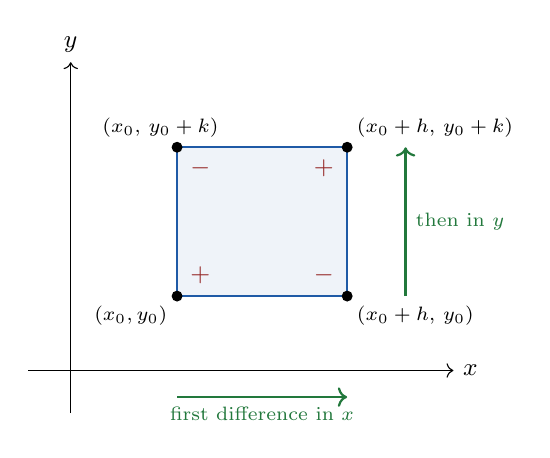
\begin{tikzpicture}[scale=1.35]
\draw[->] (-0.4,0) -- (3.6,0) node[right, font=\small] {$x$};
\draw[->] (0,-0.4) -- (0,2.9) node[above, font=\small] {$y$};
% rectangle corners
\coordinate (A) at (1.0,0.7);
\coordinate (B) at (2.6,0.7);
\coordinate (C) at (2.6,2.1);
\coordinate (D) at (1.0,2.1);
\draw[thick, figB, fill=figB!7] (A) rectangle (C);
\filldraw (A) circle (1.3pt) node[below left, font=\scriptsize] {$(x_0,y_0)$};
\filldraw (B) circle (1.3pt) node[below right, font=\scriptsize] {$(x_0+h,\,y_0)$};
\filldraw (C) circle (1.3pt) node[above right, font=\scriptsize] {$(x_0+h,\,y_0+k)$};
\filldraw (D) circle (1.3pt) node[above, font=\scriptsize, xshift=-6pt] {$(x_0,\,y_0+k)$};
% signs of the mixed second difference
\node[figR!85!black, font=\small] at ($(A)+(0.22,0.2)$) {$+$};
\node[figR!85!black, font=\small] at ($(B)+(-0.22,0.2)$) {$-$};
\node[figR!85!black, font=\small] at ($(C)+(-0.22,-0.2)$) {$+$};
\node[figR!85!black, font=\small] at ($(D)+(0.22,-0.2)$) {$-$};
% braces indicating the two difference orders
\draw[->, figG, thick] (1.0,-0.25) -- (2.6,-0.25) node[midway, below, font=\scriptsize] {first difference in $x$};
\draw[->, figG, thick] (3.15,0.7) -- (3.15,2.1) node[midway, right, font=\scriptsize] {then in $y$};
\end{tikzpicture}%
\figcap{The mixed second difference $\Delta = f(C) - f(B) - f(D) + f(A)$ (signs at the corners) is symmetric in the two directions: differencing first in $x$ then in $y$, or first in $y$ then in $x$, gives the same $\Delta$. Two applications of the Mean Value Theorem convert the two readings into $f_{xy}$ and $f_{yx}$ at interior points --- continuity forces them equal in the limit.}
\end{center}


\begin{proof}
Let $(x_0, y_0) \in R$. Since $R$ is open, there exists $r > 0$ such that $B((x_0, y_0), r) \subseteq R$.

\textbf{Motivation for $I(h,k)$:} By definition of partial derivatives,
\[
f_{xy}(x_0, y_0) = \frac{\partial}{\partial x}\left(\frac{\partial f}{\partial y}\right)\bigg|_{(x_0,y_0)} = \lim_{h \to 0} \frac{f_y(x_0 + h, y_0) - f_y(x_0, y_0)}{h}.
\]
Substituting the definition of $f_y$:
\[
f_{xy}(x_0, y_0) = \lim_{h \to 0} \lim_{k \to 0} \frac{1}{h}\left(\frac{f(x_0+h, y_0+k) - f(x_0+h, y_0)}{k} - \frac{f(x_0, y_0+k) - f(x_0, y_0)}{k}\right).
\]
Combining the fractions:
\[
f_{xy}(x_0, y_0) = \lim_{h \to 0} \lim_{k \to 0} \frac{f(x_0+h, y_0+k) - f(x_0+h, y_0) - f(x_0, y_0+k) + f(x_0, y_0)}{hk}.
\]
Similarly, $f_{yx}(x_0, y_0) = \lim_{k \to 0} \lim_{h \to 0}$ of the same expression. This motivates defining:
\[
I(h, k) = \frac{f(x_0 + h, y_0 + k) - f(x_0, y_0 + k) - f(x_0 + h, y_0) + f(x_0, y_0)}{hk}
\]
for $h, k \neq 0$ with $|h|, |k| < r/2$. The key observation is that $I(h,k)$ is symmetric in structure, and we will show it equals both $f_{xy}$ and $f_{yx}$ at nearby points.

\textbf{Expressing $I$ via $f_{xy}$:} Define $\varphi(y) = f(x_0 + h, y) - f(x_0, y)$ for $y \in [y_0, y_0 + k]$. Then
\[
I(h, k) = \frac{\varphi(y_0 + k) - \varphi(y_0)}{hk}.
\]

Since $f_y$ exists on $R$, the function $\varphi$ is differentiable with $\varphi'(y) = f_y(x_0 + h, y) - f_y(x_0, y)$. By MVT, there exists $\theta(h, k) \in [0, 1]$ such that
\[
\varphi(y_0 + k) - \varphi(y_0) = k \cdot \varphi'(y_0 + \theta(h,k) \cdot k) = k \cdot \bigl[f_y(x_0 + h, y_0 + \theta(h,k) \cdot k) - f_y(x_0, y_0 + \theta(h,k) \cdot k)\bigr].
\]
Thus
\[
I(h, k) = \frac{f_y(x_0 + h, y_0 + \theta(h,k) \cdot k) - f_y(x_0, y_0 + \theta(h,k) \cdot k)}{h}.
\]

Now define $g(x) = f_y(x, y_0 + \theta(h,k) \cdot k)$ for $x \in [x_0, x_0 + h]$. Since $f_{xy}$ exists on $R$, the function $g$ is differentiable with $g'(x) = f_{xy}(x, y_0 + \theta(h,k) \cdot k)$. By MVT, there exists $\alpha(h, k) \in [0, 1]$ such that
\[
g(x_0 + h) - g(x_0) = h \cdot g'(x_0 + \alpha(h,k) \cdot h) = h \cdot f_{xy}(x_0 + \alpha(h,k) \cdot h, y_0 + \theta(h,k) \cdot k).
\]

Therefore:
\[
I(h, k) = f_{xy}(x_0 + \alpha(h,k) \cdot h, \, y_0 + \theta(h,k) \cdot k).
\]

\textbf{Expressing $I$ via $f_{yx}$:} Define $\psi(x) = f(x, y_0 + k) - f(x, y_0)$ for $x \in [x_0, x_0 + h]$. Then
\[
I(h, k) = \frac{\psi(x_0 + h) - \psi(x_0)}{hk}.
\]

By the same argument (applying MVT twice, first in $x$, then in $y$), there exist $\beta(h, k), \gamma(h, k) \in [0, 1]$ such that
\[
I(h, k) = f_{yx}(x_0 + \beta(h,k) \cdot h, \, y_0 + \gamma(h,k) \cdot k).
\]

\textbf{Taking the limit:} Since both expressions equal $I(h, k)$:
\[
f_{xy}(x_0 + \alpha(h,k) \cdot h, y_0 + \theta(h,k) \cdot k) = f_{yx}(x_0 + \beta(h,k) \cdot h, y_0 + \gamma(h,k) \cdot k).
\]

As $(h, k) \to (0, 0)$:
\begin{itemize}[itemsep=2pt]
    \item $(x_0 + \alpha(h,k) \cdot h, y_0 + \theta(h,k) \cdot k) \to (x_0, y_0)$ since $\alpha(h,k), \theta(h,k) \in [0, 1]$
    \item $(x_0 + \beta(h,k) \cdot h, y_0 + \gamma(h,k) \cdot k) \to (x_0, y_0)$ since $\beta(h,k), \gamma(h,k) \in [0, 1]$
\end{itemize}

By continuity of $f_{xy}$ and $f_{yx}$ at $(x_0, y_0)$:
\begin{align*}
f_{xy}(x_0, y_0) &= \lim_{(h,k) \to (0,0)} f_{xy}(x_0 + \alpha(h,k) \cdot h, y_0 + \theta(h,k) \cdot k) \\
&= \lim_{(h,k) \to (0,0)} f_{yx}(x_0 + \beta(h,k) \cdot h, y_0 + \gamma(h,k) \cdot k) = f_{yx}(x_0, y_0).
\end{align*}
\end{proof}

\section{Differentiability}

\subsection*{Motivation: What Should Differentiability Mean?}

In single-variable calculus, $f: \R \to \R$ is differentiable at $x_0$ if there exists a \textbf{linear map} $L: \R \to \R$ such that
\[
f(x_0 + h) - f(x_0) = L(h) + o(h).
\]
Since every linear map $\R \to \R$ has the form $L(h) = c \cdot h$ for some constant $c$, this becomes:
\[
f(x_0 + h) - f(x_0) = f'(x_0) \cdot h + o(h).
\]

For multivariable functions $f: \R^2 \to \R$, we use the same idea: $f$ is differentiable at $(x_0, y_0)$ if there exists a \textbf{linear map} $L: \R^2 \to \R$ such that
\[
f(x_0 + h, y_0 + k) - f(x_0, y_0) = L(h, k) + o(\rho), \quad \text{where } \rho = \sqrt{h^2 + k^2}.
\]
Every linear map $\R^2 \to \R$ has the form $L(h, k) = A \cdot h + B \cdot k$ for constants $A, B$.

\begin{center}
\includegraphics[width=0.62\textwidth]{pyfigs/f2_tangent_plane.pdf}%
\figcap{Differentiability means the surface $z = f(x,y)$ has a tangent plane at the point: the graph of the linear map $L(h,k) = f_x h + f_y k$, shifted to the point of tangency. The error between surface and plane is $o(\rho)$ --- it vanishes faster than the distance.}
\end{center}

\begin{remark}[Why Not Just Require Partials to Exist?]
You might ask: why not define differentiability as ``$f_x$ and $f_y$ exist''?

The problem is that partial derivatives only measure change along the coordinate axes. Consider $f(x,y) = \frac{2xy}{x^2 + y^2}$ for $(x,y) \neq (0,0)$ and $f(0,0) = 0$. We have $f_x(0,0) = f_y(0,0) = 0$, so the ``linear approximation'' would be $L(h,k) = 0$.

But along $y = x$: $f(h, h) = 1 \neq 0$. The linear approximation is terrible in this direction!

The issue: partials exist, but they don't fit together into a coherent linear approximation for all directions.
\end{remark}

\begin{remark}[The $o(\rho)$ Condition]
The condition $E(h,k) = o(\rho)$ means:
\[
\lim_{(h,k) \to (0,0)} \frac{|E(h,k)|}{\sqrt{h^2 + k^2}} = 0.
\]
Equivalently, the definition of differentiability can be written as:
\[
\lim_{(h,k) \to (0,0)} \frac{f(x_0 + h, y_0 + k) - f(x_0, y_0) - f_x \cdot h - f_y \cdot k}{\sqrt{h^2 + k^2}} = 0.
\]
Compare with the single-variable case:
\[
\lim_{h \to 0} \frac{f(x_0 + h) - f(x_0) - f'(x_0) \cdot h}{h} = 0.
\]
The structure is identical: (actual change) $-$ (linear approximation), divided by distance.

Dividing by $\rho = \sqrt{h^2 + k^2}$ (rather than $h$ or $k$ alone) ensures the approximation is good \textbf{uniformly in all directions}.
\end{remark}

\subsection*{Formal Definition}

\begin{definition}[Differentiability]
$f : \R^2 \to \R$ is \textbf{differentiable} at $(x_0, y_0)$ if there exist constants $A, B$ such that
\[
f(x_0 + h, y_0 + k) - f(x_0, y_0) = A \cdot h + B \cdot k + o(\sqrt{h^2 + k^2}).
\]
If $f$ is differentiable, then necessarily $A = f_x(x_0, y_0)$ and $B = f_y(x_0, y_0)$.
\end{definition}

\begin{proof}[Proof that $A = f_x(x_0, y_0)$]
Setting $k = 0$: $f(x_0 + h, y_0) - f(x_0, y_0) = A \cdot h + o(|h|)$, so
\[
\frac{f(x_0 + h, y_0) - f(x_0, y_0)}{h} = A + \frac{o(|h|)}{h} \to A \quad \text{as } h \to 0.
\]
By definition of partial derivative, this limit equals $f_x(x_0, y_0)$. Hence $A = f_x(x_0, y_0)$.

Similarly, setting $h = 0$ shows $B = f_y(x_0, y_0)$.
\end{proof}


\begin{definition}[The Total Derivative and the Jacobian Matrix]
Let $f: \R^2 \to \R$ be differentiable at $(x_0, y_0)$. The \textbf{(total) derivative} of $f$ at $(x_0, y_0)$ is not a number --- it is the linear map
\[
Df_{(x_0, y_0)}: \R^2 \to \R, \quad (h, k) \mapsto f_x(x_0, y_0) \cdot h + f_y(x_0, y_0) \cdot k.
\]
Its matrix in the standard basis is the \textbf{Jacobian matrix}:
\[
Df_{(x_0, y_0)} = \begin{pmatrix} f_x & f_y \end{pmatrix}, \quad Df_{(x_0,y_0)} \begin{pmatrix} h \\ k \end{pmatrix} = f_x \cdot h + f_y \cdot k.
\]
\end{definition}

\begin{definition}[Tangent Plane]
Let $f$ be differentiable at $(x_0, y_0)$. The \textbf{tangent plane} to the graph of $f$ at $(x_0, y_0, f(x_0, y_0))$ is the plane
\[
z = f(x_0, y_0) + f_x(x_0, y_0)(x - x_0) + f_y(x_0, y_0)(y - y_0),
\]
i.e., the graph of the affine map $z = f(x_0, y_0) + L(x - x_0, y - y_0)$, where $L = Df_{(x_0,y_0)}$.
\end{definition}

\begin{remark}
Differentiability means: the tangent plane approximates $f$ well \textit{in all directions} --- the error is $o(\rho)$ uniformly, not merely along the axes.
\end{remark}

\begin{theorem}[Differentiability Implies All Directional Derivatives]
If $f$ is differentiable at $(x_0, y_0)$ with derivative $L = Df_{(x_0,y_0)}$, then for every unit direction $\mathbf{u} = (a, b)$ the directional derivative exists and
\[
D_{\mathbf{u}} f(x_0, y_0) = L(a, b) = f_x(x_0,y_0) \cdot a + f_y(x_0,y_0) \cdot b.
\]
\end{theorem}

\begin{proof}
Apply the definition of differentiability with the increment $(h, k) = (ta, tb)$:
\[
f(x_0 + ta,\, y_0 + tb) - f(x_0, y_0) = L(ta, tb) + E(ta, tb) = t \cdot L(a, b) + E(ta, tb),
\]
using linearity of $L$. Here $\rho = \sqrt{(ta)^2 + (tb)^2} = |t|\sqrt{a^2 + b^2} = |t|$, since $\mathbf{u}$ is a unit vector. Dividing by $t \neq 0$:
\[
\frac{f(x_0 + ta, y_0 + tb) - f(x_0, y_0)}{t} = L(a, b) + \frac{E(ta, tb)}{t},
\]
and
\[
\left| \frac{E(ta, tb)}{t} \right| = \frac{|E(ta, tb)|}{\rho} \to 0 \quad \text{as } t \to 0,
\]
by the $o(\rho)$ condition. Hence the limit exists and equals $L(a, b)$.
\end{proof}

\begin{remark}[Warning: The Converse Is False]
All directional derivatives can exist without $f$ being differentiable --- they might not ``fit together'' into a single linear map. The function $f(x,y) = \frac{2xy}{x^2+y^2}$ from the motivation is one witness: both partials exist at the origin, yet no linear approximation works along $y = x$.
\end{remark}

\subsection*{Summary}

\begin{center}
\begin{tabular}{|l|l|}
\hline
\textbf{Concept} & \textbf{Meaning} \\
\hline
$f$ is differentiable at $(x_0, y_0)$ & $\exists$ linear map $L$ s.t.\ $f(x_0+h, y_0+k) - f(x_0, y_0) = L(h,k) + o(\rho)$ \\
\hline
The derivative $Df$ & The linear map $L$ itself (not a number!) \\
\hline
Tangent plane & The graph of $f(x_0, y_0) + L(h, k)$ \\
\hline
Directional derivative $D_{\mathbf{u}} f$ & $L(\mathbf{u})$ --- the derivative evaluated in direction $\mathbf{u}$ \\
\hline
\end{tabular}
\end{center}

\medskip

\textbf{Differentiability = existence of a good linear approximation in ALL directions at once.}

\begin{example}[Partials Exist but Not Differentiable]
Let $f(x, y) = \dfrac{2xy}{x^2 + y^2}$ for $(x, y) \neq (0, 0)$ and $f(0, 0) = 0$.

We have $f_x(0, 0) = f_y(0, 0) = 0$. If $f$ were differentiable at $(0, 0)$:
\[
f(h, k) - f(0, 0) = 0 \cdot h + 0 \cdot k + o(\sqrt{h^2 + k^2}).
\]
But with $h = k$: $f(h, h) = 1 \neq o(\sqrt{2}|h|)$. So $f$ is \textbf{not differentiable} at $(0, 0)$.
\end{example}

\begin{theorem}[Continuous Partials Imply Differentiability]
Let $R$ be an open set. If $f_x$ and $f_y$ exist and are continuous on $R$, then $f$ is differentiable at every point of $R$.
\end{theorem}

\begin{proof}
Let $(x_0, y_0) \in R$. Since $R$ is open, there exists $r > 0$ such that $B((x_0, y_0), r) \subseteq R$.

\textbf{Goal:} Show that
\[
f(x_0 + h, y_0 + k) - f(x_0, y_0) - f_x(x_0, y_0) \cdot h - f_y(x_0, y_0) \cdot k = o(\sqrt{h^2 + k^2})
\]
as $(h, k) \to (0, 0)$.

For $(h, k)$ with $|(h, k)| < r$, define:
\[
E(h, k) = f(x_0 + h, y_0 + k) - f(x_0, y_0) - f_x(x_0, y_0) \cdot h - f_y(x_0, y_0) \cdot k.
\]

We rewrite $E(h, k)$ by adding and subtracting $f(x_0 + h, y_0)$:
\begin{align*}
E(h, k) &= \bigl[f(x_0 + h, y_0 + k) - f(x_0 + h, y_0)\bigr] + \bigl[f(x_0 + h, y_0) - f(x_0, y_0)\bigr] \\
&\qquad - f_x(x_0, y_0) \cdot h - f_y(x_0, y_0) \cdot k.
\end{align*}

\textbf{Second bracket:} Define $g(x) = f(x, y_0)$ for $x \in [x_0, x_0 + h]$. Since $f_x$ exists on $R$, the function $g$ is differentiable with $g'(x) = f_x(x, y_0)$. By MVT, there exists $\alpha(h) \in [0, 1]$ such that
\[
f(x_0 + h, y_0) - f(x_0, y_0) = h \cdot f_x(x_0 + \alpha(h) \cdot h, y_0).
\]

\textbf{First bracket:} Define $\psi(y) = f(x_0 + h, y)$ for $y \in [y_0, y_0 + k]$. Since $f_y$ exists on $R$, the function $\psi$ is differentiable with $\psi'(y) = f_y(x_0 + h, y)$. By MVT, there exists $\theta(h, k) \in [0, 1]$ such that
\[
f(x_0 + h, y_0 + k) - f(x_0 + h, y_0) = k \cdot f_y(x_0 + h, y_0 + \theta(h, k) \cdot k).
\]

Substituting into $E(h, k)$:
\begin{align*}
E(h, k) &= k \cdot f_y(x_0 + h, y_0 + \theta(h, k) \cdot k) + h \cdot f_x(x_0 + \alpha(h) \cdot h, y_0) - f_x(x_0, y_0) \cdot h - f_y(x_0, y_0) \cdot k \\
&= \bigl[f_x(x_0 + \alpha(h) \cdot h, y_0) - f_x(x_0, y_0)\bigr] \cdot h + \bigl[f_y(x_0 + h, y_0 + \theta(h, k) \cdot k) - f_y(x_0, y_0)\bigr] \cdot k.
\end{align*}

\textbf{Bounding $|E(h, k)|$:} Let $\rho = \sqrt{h^2 + k^2}$. Since $|h| \leq \rho$ and $|k| \leq \rho$:
\[
|E(h, k)| \leq \bigl|f_x(x_0 + \alpha(h) \cdot h, y_0) - f_x(x_0, y_0)\bigr| \cdot \rho + \bigl|f_y(x_0 + h, y_0 + \theta(h, k) \cdot k) - f_y(x_0, y_0)\bigr| \cdot \rho.
\]

Thus:
\[
\frac{|E(h, k)|}{\rho} \leq \bigl|f_x(x_0 + \alpha(h) \cdot h, y_0) - f_x(x_0, y_0)\bigr| + \bigl|f_y(x_0 + h, y_0 + \theta(h, k) \cdot k) - f_y(x_0, y_0)\bigr|.
\]

\textbf{Taking the limit:} As $(h, k) \to (0, 0)$:
\begin{itemize}[itemsep=2pt]
    \item $(x_0 + \alpha(h) \cdot h, y_0) \to (x_0, y_0)$ since $\alpha(h) \in [0, 1]$ and $h \to 0$
    \item $(x_0 + h, y_0 + \theta(h, k) \cdot k) \to (x_0, y_0)$ since $h \to 0$, $\theta(h,k) \in [0, 1]$, and $k \to 0$
\end{itemize}

By continuity of $f_x$ at $(x_0, y_0)$:
\[
\bigl|f_x(x_0 + \alpha(h) \cdot h, y_0) - f_x(x_0, y_0)\bigr| \to 0.
\]

By continuity of $f_y$ at $(x_0, y_0)$:
\[
\bigl|f_y(x_0 + h, y_0 + \theta(h, k) \cdot k) - f_y(x_0, y_0)\bigr| \to 0.
\]

Therefore $\dfrac{|E(h, k)|}{\rho} \to 0$ as $(h, k) \to (0, 0)$, which means $E(h, k) = o(\rho)$.

Hence $f$ is differentiable at $(x_0, y_0)$.
\end{proof}

\subsection{Algebra of Partial Derivatives}

\begin{theorem}[Partial Derivatives of Sum and Difference]
If $f_x, f_y, g_x, g_y$ exist at $(x_0, y_0)$, then $(f \pm g)_x$ and $(f \pm g)_y$ exist at $(x_0, y_0)$ and:
\[
(f \pm g)_x = f_x \pm g_x, \qquad (f \pm g)_y = f_y \pm g_y.
\]
\end{theorem}

\begin{proof}
By definition:
\begin{align*}
(f + g)_x(x_0, y_0) &= \lim_{h \to 0} \frac{(f + g)(x_0 + h, y_0) - (f + g)(x_0, y_0)}{h} \\
&= \lim_{h \to 0} \frac{f(x_0 + h, y_0) - f(x_0, y_0)}{h} + \lim_{h \to 0} \frac{g(x_0 + h, y_0) - g(x_0, y_0)}{h} \\
&= f_x(x_0, y_0) + g_x(x_0, y_0).
\end{align*}
The proofs for $(f + g)_y$, $(f - g)_x$, and $(f - g)_y$ are identical.
\end{proof}

\begin{theorem}[Product Rule for Partial Derivatives]
If $f_x, f_y, g_x, g_y$ exist at $(x_0, y_0)$, then $(fg)_x$ and $(fg)_y$ exist at $(x_0, y_0)$ and:
\[
(fg)_x = f_x g + f g_x, \qquad (fg)_y = f_y g + f g_y.
\]
\end{theorem}

\begin{proof}
We compute:
\begin{align*}
(fg)_x(x_0, y_0) &= \lim_{h \to 0} \frac{f(x_0 + h, y_0) g(x_0 + h, y_0) - f(x_0, y_0) g(x_0, y_0)}{h}.
\end{align*}
Add and subtract $f(x_0 + h, y_0) g(x_0, y_0)$:
\begin{align*}
&= \lim_{h \to 0} \frac{f(x_0 + h, y_0) [g(x_0 + h, y_0) - g(x_0, y_0)] + g(x_0, y_0) [f(x_0 + h, y_0) - f(x_0, y_0)]}{h} \\
&= \lim_{h \to 0} f(x_0 + h, y_0) \cdot \frac{g(x_0 + h, y_0) - g(x_0, y_0)}{h} + g(x_0, y_0) \cdot \lim_{h \to 0} \frac{f(x_0 + h, y_0) - f(x_0, y_0)}{h}.
\end{align*}
Since $f_x$ exists, $f$ is continuous in $x$ at $(x_0, y_0)$, so $\lim_{h \to 0} f(x_0 + h, y_0) = f(x_0, y_0)$. Thus:
\[
(fg)_x(x_0, y_0) = f(x_0, y_0) \cdot g_x(x_0, y_0) + g(x_0, y_0) \cdot f_x(x_0, y_0).
\]
The proof for $(fg)_y$ is identical.
\end{proof}

\begin{theorem}[Quotient Rule for Partial Derivatives]
If $f_x, f_y, g_x, g_y$ exist at $(x_0, y_0)$ and $g(x_0, y_0) \neq 0$, then $(f/g)_x$ and $(f/g)_y$ exist at $(x_0, y_0)$ and:
\[
\left(\frac{f}{g}\right)_x = \frac{f_x g - f g_x}{g^2}, \qquad \left(\frac{f}{g}\right)_y = \frac{f_y g - f g_y}{g^2}.
\]
\end{theorem}

\begin{proof}
First, we show $(1/g)_x = -g_x / g^2$. We have:
\begin{align*}
\left(\frac{1}{g}\right)_x(x_0, y_0) &= \lim_{h \to 0} \frac{\frac{1}{g(x_0 + h, y_0)} - \frac{1}{g(x_0, y_0)}}{h} \\
&= \lim_{h \to 0} \frac{g(x_0, y_0) - g(x_0 + h, y_0)}{h \cdot g(x_0 + h, y_0) \cdot g(x_0, y_0)} \\
&= \frac{-g_x(x_0, y_0)}{g(x_0, y_0)^2}.
\end{align*}
(We used continuity of $g$ in $x$, which follows from existence of $g_x$.)

Now apply the product rule to $f \cdot (1/g)$:
\[
\left(\frac{f}{g}\right)_x = f_x \cdot \frac{1}{g} + f \cdot \left(-\frac{g_x}{g^2}\right) = \frac{f_x}{g} - \frac{f g_x}{g^2} = \frac{f_x g - f g_x}{g^2}.
\]
The proof for $(f/g)_y$ is identical.
\end{proof}

\subsection{Algebra of Differentiable Functions}

\begin{theorem}[Sum and Difference of Differentiable Functions]
If $f$ and $g$ are differentiable at $(x_0, y_0)$, then $f + g$ and $f - g$ are differentiable at $(x_0, y_0)$.
\end{theorem}

\begin{proof}
Since $f$ is differentiable at $(x_0, y_0)$:
\[
f(x_0 + h, y_0 + k) - f(x_0, y_0) = f_x(x_0, y_0) h + f_y(x_0, y_0) k + o(\rho).
\]
Since $g$ is differentiable at $(x_0, y_0)$:
\[
g(x_0 + h, y_0 + k) - g(x_0, y_0) = g_x(x_0, y_0) h + g_y(x_0, y_0) k + o(\rho).
\]
Adding these:
\begin{align*}
(f + g)(x_0 + h, y_0 + k) - (f + g)(x_0, y_0) &= (f_x + g_x) h + (f_y + g_y) k + o(\rho).
\end{align*}
This is exactly the definition of differentiability for $f + g$, with partial derivatives $f_x + g_x$ and $f_y + g_y$.
\end{proof}

\begin{theorem}[Product of Differentiable Functions]
If $f$ and $g$ are differentiable at $(x_0, y_0)$, then $fg$ is differentiable at $(x_0, y_0)$.
\end{theorem}

\begin{proof}
Let $f_0 = f(x_0, y_0)$, $g_0 = g(x_0, y_0)$, and write:
\begin{align*}
f(x_0 + h, y_0 + k) &= f_0 + f_x h + f_y k + o(\rho) =: f_0 + \Delta f, \\
g(x_0 + h, y_0 + k) &= g_0 + g_x h + g_y k + o(\rho) =: g_0 + \Delta g.
\end{align*}
where $\Delta f = f_x h + f_y k + o(\rho)$ and $\Delta g = g_x h + g_y k + o(\rho)$.

Then:
\begin{align*}
(fg)(x_0 + h, y_0 + k) - (fg)(x_0, y_0) &= (f_0 + \Delta f)(g_0 + \Delta g) - f_0 g_0 \\
&= f_0 \Delta g + g_0 \Delta f + \Delta f \cdot \Delta g.
\end{align*}

Now:
\begin{align*}
f_0 \Delta g + g_0 \Delta f &= f_0 (g_x h + g_y k) + g_0 (f_x h + f_y k) + o(\rho) \\
&= (f_0 g_x + g_0 f_x) h + (f_0 g_y + g_0 f_y) k + o(\rho) \\
&= (fg)_x h + (fg)_y k + o(\rho).
\end{align*}

For the remaining term, note that $|\Delta f| \leq C\rho$ and $|\Delta g| \leq C\rho$ for some constant $C$ (since linear terms plus $o(\rho)$ are $O(\rho)$). Thus:
\[
|\Delta f \cdot \Delta g| \leq C^2 \rho^2 = o(\rho).
\]

Therefore:
\[
(fg)(x_0 + h, y_0 + k) - (fg)(x_0, y_0) = (fg)_x h + (fg)_y k + o(\rho).
\]
Hence $fg$ is differentiable at $(x_0, y_0)$.
\end{proof}

\begin{theorem}[Quotient of Differentiable Functions]
If $f$ and $g$ are differentiable at $(x_0, y_0)$ and $g(x_0, y_0) \neq 0$, then $f/g$ is differentiable at $(x_0, y_0)$.
\end{theorem}

\begin{proof}
It suffices to show $1/g$ is differentiable (then apply the product rule to $f \cdot (1/g)$).

Let $g_0 = g(x_0, y_0) \neq 0$. Since $g$ is differentiable:
\[
g(x_0 + h, y_0 + k) = g_0 + g_x h + g_y k + o(\rho) = g_0(1 + \epsilon),
\]
where $\epsilon = \frac{g_x h + g_y k + o(\rho)}{g_0} = O(\rho)/g_0$.

For small $\rho$, $|\epsilon| < 1$, so we can use $\frac{1}{1 + \epsilon} = 1 - \epsilon + O(\epsilon^2)$:
\begin{align*}
\frac{1}{g(x_0 + h, y_0 + k)} &= \frac{1}{g_0(1 + \epsilon)} = \frac{1}{g_0}(1 - \epsilon + O(\epsilon^2)) \\
&= \frac{1}{g_0} - \frac{1}{g_0} \cdot \frac{g_x h + g_y k + o(\rho)}{g_0} + O(\rho^2) \\
&= \frac{1}{g_0} - \frac{g_x}{g_0^2} h - \frac{g_y}{g_0^2} k + o(\rho).
\end{align*}

Thus:
\[
\frac{1}{g(x_0 + h, y_0 + k)} - \frac{1}{g(x_0, y_0)} = -\frac{g_x}{g^2} h - \frac{g_y}{g^2} k + o(\rho).
\]
This shows $1/g$ is differentiable with $(1/g)_x = -g_x/g^2$ and $(1/g)_y = -g_y/g^2$.
\end{proof}

\begin{theorem}[Chain Rule: Composition of Differentiable Functions]
Let $g(x,y) = f(\varphi(x,y), \psi(x,y))$. If $\varphi, \psi$ are differentiable at $(x_0, y_0)$ and $f$ is differentiable at $(\varphi(x_0, y_0), \psi(x_0, y_0))$, then $g$ is differentiable at $(x_0, y_0)$ with:
\[
g_x = f_\xi \varphi_x + f_\eta \psi_x, \qquad g_y = f_\xi \varphi_y + f_\eta \psi_y.
\]
\end{theorem}

\begin{proof}
Let $(\xi_0, \eta_0) = (\varphi(x_0, y_0), \psi(x_0, y_0))$. Since $\varphi, \psi$ are differentiable at $(x_0, y_0)$:
\begin{align*}
\varphi(x_0 + h, y_0 + k) - \varphi(x_0, y_0) &= \varphi_x h + \varphi_y k + o(\rho) =: \Delta\xi, \\
\psi(x_0 + h, y_0 + k) - \psi(x_0, y_0) &= \psi_x h + \psi_y k + o(\rho) =: \Delta\eta.
\end{align*}

Note that $|\Delta\xi|, |\Delta\eta| = O(\rho)$, so $\sigma := \sqrt{(\Delta\xi)^2 + (\Delta\eta)^2} = O(\rho)$.

Since $f$ is differentiable at $(\xi_0, \eta_0)$:
\[
f(\xi_0 + \Delta\xi, \eta_0 + \Delta\eta) - f(\xi_0, \eta_0) = f_\xi \Delta\xi + f_\eta \Delta\eta + o(\sigma).
\]

Since $\sigma = O(\rho)$, we have $o(\sigma) = o(\rho)$. Substituting:
\begin{align*}
g(x_0 + h, y_0 + k) - g(x_0, y_0) &= f_\xi (\varphi_x h + \varphi_y k + o(\rho)) + f_\eta (\psi_x h + \psi_y k + o(\rho)) + o(\rho) \\
&= (f_\xi \varphi_x + f_\eta \psi_x) h + (f_\xi \varphi_y + f_\eta \psi_y) k + o(\rho).
\end{align*}

Hence $g$ is differentiable with the stated partial derivatives.
\end{proof}

\begin{remark}[Summary: Algebra of Differentiable Functions]
If $f$ and $g$ are differentiable at $(x_0, y_0)$:
\begin{center}
\begin{tabular}{|c|c|c|}
\hline
\textbf{Function} & \textbf{Differentiable?} & \textbf{Partial Derivatives} \\
\hline
$f + g$ & Yes & $(f+g)_x = f_x + g_x$, \; $(f+g)_y = f_y + g_y$ \\
\hline
$f - g$ & Yes & $(f-g)_x = f_x - g_x$, \; $(f-g)_y = f_y - g_y$ \\
\hline
$fg$ & Yes & $(fg)_x = f_x g + f g_x$, \; $(fg)_y = f_y g + f g_y$ \\
\hline
$f/g$ & Yes (if $g \neq 0$) & $(f/g)_x = \dfrac{f_x g - f g_x}{g^2}$, \; $(f/g)_y = \dfrac{f_y g - f g_y}{g^2}$ \\
\hline
$h(f, g)$ & Yes (if $h$ diff.) & Chain rule \\
\hline
\end{tabular}
\end{center}
\end{remark}

\section{Directional Derivatives}

A basic property of differentiable functions $f$ is that they not only possess partial derivatives with respect to $x$ and $y$ — or, as we also say, in the $x$- and $y$-directions — but that they have derivatives in \textbf{any direction}, and these derivatives can all be expressed in terms of $f_x$ and $f_y$.

\begin{definition}[Directional Derivative]
By the \textbf{derivative in the direction $\alpha$} we mean the rate of change of $f$ at the point $(x, y)$ with respect to distance as we approach $(x, y)$ along the ray that forms the angle $\alpha$ with the positive $x$-axis.

The points $(x + h, y + k)$ along this ray have the form
\[
h = \rho \cos \alpha, \qquad k = \rho \sin \alpha,
\]
where $\rho = \sqrt{h^2 + k^2}$ is the distance from $(x + h, y + k)$ to $(x, y)$.

Along this ray, $f$ becomes a function of $\rho$:
\[
f(x + \rho \cos \alpha, \, y + \rho \sin \alpha).
\]

The \textbf{directional derivative} of $f$ at $(x, y)$ in the direction $\alpha$ is defined as:
\[
D_{(\alpha)} f(x, y) = \left( \frac{d}{d\rho} f(x + \rho \cos \alpha, \, y + \rho \sin \alpha) \right)\bigg|_{\rho = 0} = \lim_{\rho \to 0} \frac{f(x + \rho \cos \alpha, \, y + \rho \sin \alpha) - f(x, y)}{\rho},
\]
provided the limit exists.
\end{definition}

\begin{center}
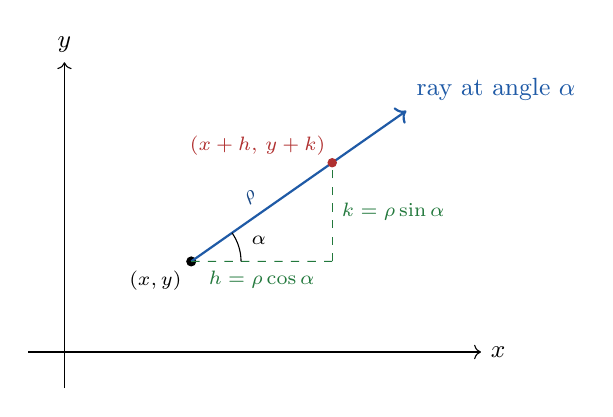
\begin{tikzpicture}[scale=1.15]
% domain plane
\draw[->] (-0.4,0) -- (4.6,0) node[right, font=\small] {$x$};
\draw[->] (0,-0.4) -- (0,3.2) node[above, font=\small] {$y$};
% base point
\coordinate (P) at (1.4,1.0);
\filldraw (P) circle (1.4pt) node[below left, font=\scriptsize] {$(x,y)$};
% ray at angle alpha = 35 deg
\draw[->, thick, figB] (P) -- ++(35:2.9) node[above right, font=\small] {ray at angle $\alpha$};
% moving point at distance rho
\coordinate (Q) at ($(P)+(35:1.9)$);
\filldraw[figR] (Q) circle (1.3pt) node[above left=-1pt, font=\scriptsize] {$(x+h,\,y+k)$};
% rho label along ray
\node[figB!80!black, font=\scriptsize, rotate=35] at ($(P)+(35:0.95)+(-0.12,0.16)$) {$\rho$};
% decompose h and k
\coordinate (H) at ($(P)+({1.9*cos(35)},0)$);
\draw[dashed, figG] (P) -- (H) node[midway, below, font=\scriptsize] {$h = \rho\cos\alpha$};
\draw[dashed, figG] (H) -- (Q) node[midway, right, font=\scriptsize] {$k = \rho\sin\alpha$};
% angle mark
\draw[thin] ($(P)+(0.55,0)$) arc[start angle=0, end angle=35, radius=0.55];
\node[font=\scriptsize] at ($(P)+(17:0.78)$) {$\alpha$};
\end{tikzpicture}%
\figcap{The directional derivative restricts $f$ to a ray: points along the direction $\alpha$ have the form $(x + \rho\cos\alpha,\, y + \rho\sin\alpha)$, turning $f$ into a single-variable function of the distance $\rho$. Its derivative at $\rho = 0$ is $D_{(\alpha)}f$. The partials are the special cases $\alpha = 0$ and $\alpha = \pi/2$.}
\end{center}


\begin{remark}[Partial Derivatives as Special Cases]
The partial derivatives are directional derivatives in the coordinate directions:
\begin{align*}
D_{(0)} f(x, y) &= \lim_{\rho \to 0} \frac{f(x + \rho, y) - f(x, y)}{\rho} = f_x(x, y), \\[6pt]
D_{(\pi/2)} f(x, y) &= \lim_{\rho \to 0} \frac{f(x, y + \rho) - f(x, y)}{\rho} = f_y(x, y).
\end{align*}
\end{remark}

\begin{theorem}[Directional Derivative Formula]
If $f(x, y)$ is differentiable at $(x, y)$, then the directional derivative in direction $\alpha$ exists and is given by:
\[
D_{(\alpha)} f(x, y) = f_x(x, y) \cos \alpha + f_y(x, y) \sin \alpha.
\]
\end{theorem}

\begin{proof}
Since $f$ is differentiable, we have:
\[
f(x + h, y + k) - f(x, y) = h f_x + k f_y + \varepsilon \rho,
\]
where $\varepsilon \to 0$ as $\rho = \sqrt{h^2 + k^2} \to 0$.

Substituting $h = \rho \cos \alpha$ and $k = \rho \sin \alpha$:
\[
f(x + \rho \cos \alpha, y + \rho \sin \alpha) - f(x, y) = \rho \cos \alpha \cdot f_x + \rho \sin \alpha \cdot f_y + \varepsilon \rho = \rho (f_x \cos \alpha + f_y \sin \alpha + \varepsilon).
\]

Dividing by $\rho$ and taking $\rho \to 0$:
\[
D_{(\alpha)} f(x, y) = \lim_{\rho \to 0} \frac{f(x + \rho \cos \alpha, y + \rho \sin \alpha) - f(x, y)}{\rho} = f_x \cos \alpha + f_y \sin \alpha + \lim_{\rho \to 0} \varepsilon = f_x \cos \alpha + f_y \sin \alpha.
\]
\end{proof}

\begin{remark}[Unit Vector Notation]
If $\mathbf{u} = (a, b)$ is a \textbf{unit vector} (so $a^2 + b^2 = 1$), we can write $a = \cos \alpha$ and $b = \sin \alpha$ for some angle $\alpha$. Then:
\[
D_{\mathbf{u}} f(x, y) = f_x(x, y) \cdot a + f_y(x, y) \cdot b = \nabla f \cdot \mathbf{u},
\]
where $\nabla f = (f_x, f_y)$ is the \textbf{gradient} of $f$.
\end{remark}

\begin{remark}[Gradient and Maximum Rate of Change]
The directional derivative $D_{(\alpha)} f = f_x \cos \alpha + f_y \sin \alpha = |\nabla f| \cos(\alpha - \theta)$, where $\theta$ is the angle of the gradient vector.

This is maximized when $\alpha = \theta$, i.e., when we move in the direction of the gradient. The maximum rate of change is $|\nabla f| = \sqrt{f_x^2 + f_y^2}$.
\end{remark}

\begin{center}
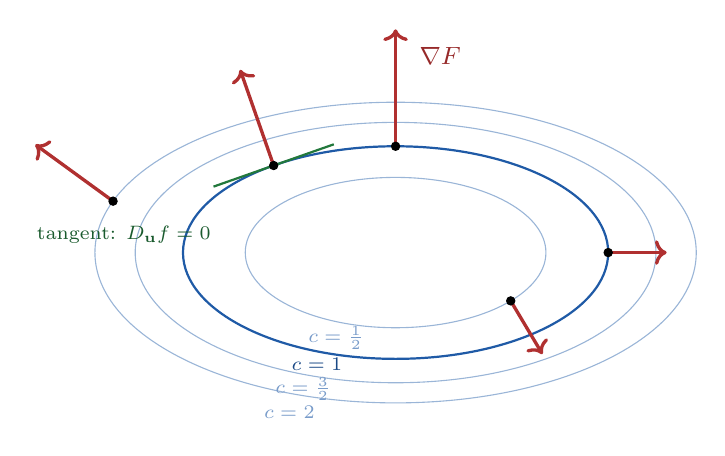
\begin{tikzpicture}[scale=1.35]
% contours of F = x^2/4 + y^2 at c = 0.5, 1, 1.5, 2  -> semi-axes (2sqrt(c), sqrt(c))
\foreach \c/\sty in {0.5/{figB!45}, 1.5/{figB!45}, 2/{figB!45}}
  \draw[\sty, thin] (0,0) ellipse ({2*sqrt(\c)} and {sqrt(\c)});
\draw[figB, thick] (0,0) ellipse ({2*sqrt(1)} and {sqrt(1)});
\node[figB!60, font=\scriptsize] at (-0.56,-0.80) {$c=\tfrac12$};
\node[figB!80!black, font=\scriptsize] at (-0.74,-1.05) {$c=1$};
\node[figB!60, font=\scriptsize] at (-0.87,-1.28) {$c=\tfrac32$};
\node[figB!60, font=\scriptsize] at (-1.00,-1.50) {$c=2$};
% gradient nabla F = (x/2, 2y); draw at several points, scaled by 0.55
% point A: (2,0) on c=1  -> grad (1,0), len 1
\draw[->, very thick, figR] (2,0) -- ++(0.55,0);
% point B: (0,1) on c=1 -> grad (0,2), len 2 (twice as long: contours twice as dense vertically)
\draw[->, very thick, figR] (0,1) -- ++(0,1.1);
% point C: on c=1 at t=125deg: (2cos125, sin125)=(-1.147,0.819); grad=(-0.574,1.638)
\draw[->, very thick, figR] (-1.147,0.819) -- ++(-0.315,0.900);
% point D: on c=0.5 at t=-40deg: (2*0.707*cos(-40), 0.707*sin(-40))=(1.083,-0.4545); grad=(0.542,-0.909)
\draw[->, very thick, figR] (1.083,-0.4545) -- ++(0.298,-0.500);
% point E: on c=2 at t=160: (2*1.414*cos160, 1.414*sin160)=(-2.658,0.4836); grad=(-1.329,0.967)
\draw[->, very thick, figR] (-2.658,0.4836) -- ++(-0.731,0.532);
\node[figR!85!black, font=\small] at (0.42,1.85) {$\nabla F$};
% one tangent segment at point B' on c=1 to show D_u f = 0 along contour
\coordinate (Pc) at (-1.147,0.819);
\draw[figG, thick] ($(Pc)+(0.566,0.199)$) -- ($(Pc)-(0.566,0.199)$);
\node[figG!75!black, font=\scriptsize, anchor=north east] at ($(Pc)-(0.50,0.48)$) {tangent: $D_{\mathbf{u}}f = 0$};
\filldraw (2,0) circle (1.1pt); \filldraw (0,1) circle (1.1pt);
\filldraw (-1.147,0.819) circle (1.1pt); \filldraw (1.083,-0.4545) circle (1.1pt);
\filldraw (-2.658,0.4836) circle (1.1pt);
\end{tikzpicture}%
\figcap{The gradient as a field on the contour map of $F = x^2/4 + y^2$. At every point, $\nabla F = (x/2,\,2y)$ is perpendicular to the contour through that point and points toward higher values. Its length encodes steepness: at $(0,1)$ the contours are packed twice as tightly as at $(2,0)$, and the gradient is exactly twice as long. Along any contour the tangential directional derivative vanishes (green tangent) --- moving along a level curve changes nothing; moving across contours, the shorter the crossing distance, the larger $|\nabla F|$.}
\end{center}

\section{The Differential}

\subsection*{What is the Differential?}

The notation $df = f'(x) \, dx$ is familiar from single-variable calculus, but what does it actually \textbf{mean}? The professor emphasizes: \textbf{the derivative $f'(x)$ is defined before the differential}.

\begin{remark}[Single Variable: The Differential as a Function]
For $f: \R \to \R$, we first define the derivative:
\[
f'(x) = \lim_{h \to 0} \frac{f(x + h) - f(x)}{h}.
\]
Then we \textbf{define} the differential $df$ as a function of \textbf{two variables} $(x, h)$:
\[
df\big|_{(x, h)} = f'(x) \cdot h.
\]
What about $dx$? Consider the identity function $r(x) = x$. Its differential is:
\[
dr\big|_{(x, h)} = r'(x) \cdot h = 1 \cdot h = h.
\]
So $dx = h$, and we can write $df = f'(x) \cdot dx$.

\textbf{Key insight:} The differential $df$ is a \textbf{linear function in the increment $h$}, not just a symbol.
\end{remark}

\begin{definition}[Differential in Multivariable Calculus]
For $f : \R^2 \to \R$, the \textbf{differential} $df$ is a function of \textbf{four variables} $(x, y, h, k)$:
\[
df\big|_{(x, y, h, k)} = f_x(x, y) \cdot h + f_y(x, y) \cdot k.
\]
Since $dx = h$ and $dy = k$ (by the same reasoning as above), we write:
\[
df = f_x \, dx + f_y \, dy.
\]
\end{definition}

\begin{remark}[Connection to Differentiability]
The differential $df$ is precisely the \textbf{linear map} $L(h, k) = f_x \cdot h + f_y \cdot k$ from our definition of differentiability!

Differentiability says:
\[
f(x_0 + h, y_0 + k) - f(x_0, y_0) = df\big|_{(x_0, y_0, h, k)} + o(\rho).
\]
So the differential $df$ is the ``best linear approximation'' to the change in $f$.
\end{remark}

\begin{note}[Looking Ahead]
The symbols $dx$ and $dy$ are defined here as ``the increment $h$ and $k$.'' In Part III (\S20--\S22), we will see that $dx$ and $dy$ are more precisely \textit{1-forms}: machines that eat a tangent vector and extract its components. The differential $df = f_x\,dx + f_y\,dy$ is then a 1-form that eats a tangent vector $\mathbf{v}$ and outputs the directional derivative $\nabla f \cdot \mathbf{v}$. The two viewpoints --- ``best linear approximation'' and ``1-form'' --- are the same object.
\end{note}

\subsection{Higher Differentials}

\begin{definition}[Second Differential]
The \textbf{second differential} is $d^2f = d(df)$. To compute it, we apply $d$ to $df = f_x \cdot h + f_y \cdot k$, treating $h$ and $k$ as constants:
\[
d^2f = d(f_x \cdot h + f_y \cdot k) = d(f_x) \cdot h + d(f_y) \cdot k.
\]

Compute each piece:
\begin{align*}
d(f_x) &= (f_x)_x \cdot h + (f_x)_y \cdot k = f_{xx} \cdot h + f_{xy} \cdot k, \\
d(f_y) &= (f_y)_x \cdot h + (f_y)_y \cdot k = f_{yx} \cdot h + f_{yy} \cdot k.
\end{align*}

Substituting:
\begin{align*}
d^2f &= (f_{xx} h + f_{xy} k) \cdot h + (f_{yx} h + f_{yy} k) \cdot k \\
&= f_{xx} h^2 + f_{xy} hk + f_{yx} hk + f_{yy} k^2.
\end{align*}

If $f_{xy} = f_{yx}$ (by Schwarz--Clairaut), then:
\[
d^2f = f_{xx} h^2 + 2f_{xy} hk + f_{yy} k^2.
\]
\end{definition}

\begin{remark}[Interpretation of $d^2f$]
The second differential $d^2f$ is a \textbf{quadratic form} in $(h, k)$. It captures the \textbf{curvature} or second-order behavior of $f$:
\begin{itemize}[itemsep=2pt]
    \item It appears in the second-order Taylor expansion of $f$.
    \item It determines whether a critical point is a local max, local min, or saddle point.
\end{itemize}
\end{remark}

\begin{definition}[Higher Differentials]
For well-behaved functions (with continuous higher partials), the $n$-th differential is:
\[
d^n f = \sum_{i=0}^{n} \binom{n}{i} \frac{\partial^n f}{\partial x^i \, \partial y^{n-i}} h^i k^{n-i}.
\]
This is a homogeneous polynomial of degree $n$ in $(h, k)$, and it appears in the $n$-th order Taylor expansion.
\end{definition}

\begin{remark}[Symbolic Interpretation]
The formula for $d^n f$ can be written symbolically as:
\[
d^n f = \left( h \frac{\partial}{\partial x} + k \frac{\partial}{\partial y} \right)^n f,
\]
where we expand the power using the binomial theorem and then apply the resulting differential operators to $f$.
\end{remark}

\subsection*{Summary}

\begin{center}
\begin{tabular}{|l|l|l|}
\hline
\textbf{Object} & \textbf{Formula} & \textbf{Interpretation} \\
\hline
$df$ & $f_x h + f_y k$ & Linear approximation (tangent plane) \\
\hline
$d^2f$ & $f_{xx} h^2 + 2f_{xy} hk + f_{yy} k^2$ & Quadratic form (curvature) \\
\hline
$d^n f$ & $\displaystyle\sum_{i=0}^{n} \binom{n}{i} \partial_x^i \partial_y^{n-i} f \cdot h^i k^{n-i}$ & $n$-th order Taylor term \\
\hline
\end{tabular}
\end{center}

\textbf{The differential is not just notation --- it is a function (linear map, quadratic form, etc.) that captures how $f$ changes to various orders.}

\section{Taylor's Theorem for Multivariable Functions}

\subsection*{Review: Single-Variable Taylor's Theorem}

For a function $f: \R \to \R$ that is $(N+1)$-times differentiable, the Taylor expansion around $x = a$ is:
\[
f(x) = \sum_{k=0}^{N} \frac{f^{(k)}(a)}{k!}(x - a)^k + R_{N+1},
\]
where the remainder (Lagrange form) is:
\[
R_{N+1} = \frac{f^{(N+1)}(\xi)}{(N+1)!}(x - a)^{N+1}
\]
for some $\xi$ between $a$ and $x$.

\subsection*{The Key Idea: Reduce to Single Variable}

For $f(x, y)$, we want to expand $f(x + h, y + k)$ around $(x, y)$. The trick is to \textbf{parametrize the line segment} from $(x, y)$ to $(x + h, y + k)$.

Define the single-variable function:
\[
F(t) = f(x + th, y + tk), \quad 0 \leq t \leq 1.
\]

\begin{center}
\begin{tikzpicture}[scale=1.5]
\draw[->] (0,0) -- (3,0) node[right] {$x$};
\draw[->] (0,0) -- (0,2.5) node[above] {$y$};
\node[circle, fill, inner sep=1.5pt, label=below left:{$(x,y)$}] at (0.5,0.5) {};
\node[circle, fill, inner sep=1.5pt, label=above right:{$(x+h,y+k)$}] at (2.5,2) {};
\draw[thick, ->, blue] (0.5,0.5) -- (2.5,2);
\node[blue] at (1.8,0.9) {$t \in [0,1]$};
\end{tikzpicture}
\end{center}

Key observations:
\begin{itemize}[itemsep=2pt]
    \item $F(0) = f(x, y)$ — the starting point
    \item $F(1) = f(x + h, y + k)$ — the ending point (what we want to expand)
\end{itemize}

Now we apply single-variable Taylor to $F(t)$ around $t = 0$!

\subsection*{Computing Derivatives of $F(t)$}

\begin{theorem}[Derivatives of $F(t)$]
If $f$ has continuous partial derivatives up to order $m$, then:
\[
F^{(m)}(t) = \sum_{\ell=0}^{m} \binom{m}{\ell} \frac{\partial^m f}{\partial x^\ell \, \partial y^{m-\ell}}(x + th, y + tk) \cdot h^\ell k^{m-\ell}.
\]
\end{theorem}

\begin{proof}
We prove by induction on $m$.

\textbf{Base case ($m = 1$):} By the chain rule:
\[
F'(t) = \frac{d}{dt} f(x + th, y + tk) = f_x(x + th, y + tk) \cdot h + f_y(x + th, y + tk) \cdot k.
\]
This matches the formula with $\binom{1}{0} = \binom{1}{1} = 1$.

\textbf{Inductive step:} Assume the formula holds for $m$. Differentiating:
\begin{align*}
F^{(m+1)}(t) &= \frac{d}{dt} F^{(m)}(t) = \frac{d}{dt} \sum_{\ell=0}^{m} \binom{m}{\ell} \frac{\partial^m f}{\partial x^\ell \, \partial y^{m-\ell}} \cdot h^\ell k^{m-\ell}.
\end{align*}

Applying the chain rule to each term:
\[
\frac{d}{dt} \frac{\partial^m f}{\partial x^\ell \, \partial y^{m-\ell}} = \frac{\partial^{m+1} f}{\partial x^{\ell+1} \, \partial y^{m-\ell}} \cdot h + \frac{\partial^{m+1} f}{\partial x^\ell \, \partial y^{m+1-\ell}} \cdot k.
\]

After collecting terms and using the Pascal's triangle identity $\binom{m}{\ell-1} + \binom{m}{\ell} = \binom{m+1}{\ell}$, we obtain the formula for $m + 1$.
\end{proof}

\begin{remark}[First Few Derivatives]
Explicitly:
\begin{align*}
F'(t) &= f_x h + f_y k, \\[4pt]
F''(t) &= f_{xx} h^2 + 2f_{xy} hk + f_{yy} k^2, \\[4pt]
F'''(t) &= f_{xxx} h^3 + 3f_{xxy} h^2 k + 3f_{xyy} hk^2 + f_{yyy} k^3,
\end{align*}
where all partial derivatives are evaluated at $(x + th, y + tk)$.

Note the binomial coefficients! This is why we can write symbolically:
\[
F^{(m)}(t) = \left( h \frac{\partial}{\partial x} + k \frac{\partial}{\partial y} \right)^m f \bigg|_{(x+th, y+tk)}.
\]
\end{remark}

\subsection{Taylor's Theorem for Two Variables}

\begin{theorem}[Multivariable Taylor's Theorem]
Let $f : \R^2 \to \R$ have continuous partial derivatives up to order $N + 1$ in a neighborhood of $(x, y)$. Then:
\[
f(x + h, y + k) = \sum_{m=0}^{N} \frac{1}{m!} \sum_{\ell=0}^{m} \binom{m}{\ell} \frac{\partial^m f}{\partial x^\ell \, \partial y^{m-\ell}}(x, y) \cdot h^\ell k^{m-\ell} + R_{N+1},
\]
where the remainder is:
\[
R_{N+1} = \frac{1}{(N+1)!} \sum_{\ell=0}^{N+1} \binom{N+1}{\ell} \frac{\partial^{N+1} f}{\partial x^\ell \, \partial y^{N+1-\ell}}(x + \theta h, y + \theta k) \cdot h^\ell k^{N+1-\ell}
\]
for some $\theta \in (0, 1)$.
\end{theorem}

\begin{proof}
Apply single-variable Taylor's theorem to $F(t) = f(x + th, y + tk)$:
\[
F(1) = \sum_{m=0}^{N} \frac{F^{(m)}(0)}{m!} \cdot 1^m + \frac{F^{(N+1)}(\theta)}{(N+1)!} \cdot 1^{N+1}
\]
for some $\theta \in (0, 1)$.

Since $F(1) = f(x + h, y + k)$ and $F^{(m)}(0)$ is the formula for derivatives evaluated at $t = 0$ (i.e., at $(x, y)$), we obtain the result.
\end{proof}

\begin{remark}[Compact Notation Using Differentials]
The Taylor expansion can be written elegantly as:
\[
f(x + h, y + k) = \sum_{m=0}^{N} \frac{1}{m!} d^m f \big|_{(x,y)} + R_{N+1},
\]
where $d^m f = \left( h \partial_x + k \partial_y \right)^m f$ is the $m$-th differential.
\end{remark}

\begin{remark}[Why the Linear Path?]
One might ask: why parametrize with the linear path $F(t) = f(x + th, y + tk)$ rather than a general path $(h(t), k(t))$ from $(0,0)$ to $(h,k)$?

The answer is that the Taylor polynomial $T_N(h,k)$ is the \textbf{unique polynomial that matches all partial derivatives of $f$ at $(x,y)$} up to order $N$. The linear path is special because:
\begin{itemize}[itemsep=2pt]
    \item The ``instantaneous direction'' $(h'(t), k'(t)) = (h, k)$ is constant
    \item No path curvature: $h^{(j)}(t) = k^{(j)}(t) = 0$ for $j \geq 2$
    \item Therefore $F^{(m)}(0) = d^m f$ directly, with no correction terms
\end{itemize}

A curved path would have a changing instantaneous direction, introducing terms involving $h''(0), k''(0), \ldots$ that mix the geometry of the path with the geometry of $f$. The final answer $f(x+h,y+k)$ is path-independent (it's just a number!), but only the linear path produces the \textbf{canonical} polynomial whose coefficients are the intrinsic partial derivatives of $f$.
\end{remark}

\subsection{Explicit Low-Order Expansions}

\begin{example}[First-Order Taylor Expansion]
For $N = 0$:
\[
f(x + h, y + k) = f(x, y) + R_1,
\]
where $R_1 = f_x(x + \theta h, y + \theta k) \cdot h + f_y(x + \theta h, y + \theta k) \cdot k$.

This is the \textbf{Mean Value Theorem} for two variables.
\end{example}

\begin{example}[Second-Order Taylor Expansion]
For $N = 1$:
\[
f(x + h, y + k) = f(x, y) + f_x(x, y) h + f_y(x, y) k + R_2,
\]
where:
\[
R_2 = \frac{1}{2} \left[ f_{xx}(\xi, \eta) h^2 + 2f_{xy}(\xi, \eta) hk + f_{yy}(\xi, \eta) k^2 \right]
\]
for some $(\xi, \eta) = (x + \theta h, y + \theta k)$ with $\theta \in (0, 1)$.

This shows that $f(x+h, y+k) = f(x,y) + df + O(\rho^2)$, confirming our definition of differentiability.
\end{example}

\begin{example}[Third-Order Taylor Expansion]
For $N = 2$:
\begin{align*}
f(x + h, y + k) &= f(x, y) + \bigl[ f_x h + f_y k \bigr] \\
&\quad + \frac{1}{2} \bigl[ f_{xx} h^2 + 2f_{xy} hk + f_{yy} k^2 \bigr] + R_3,
\end{align*}
where $R_3 = O(\rho^3)$ involves third-order partial derivatives.
\end{example}

\subsection{Appendix: Rolle's Theorem and the Mean Value Theorem}

The Taylor theorem relies on the single-variable MVT, which in turn follows from Rolle's theorem.

\begin{theorem}[Rolle's Theorem]
If $f$ is continuous on $[a, b]$, differentiable on $(a, b)$, and $f(a) = f(b)$, then there exists $\xi \in (a, b)$ such that $f'(\xi) = 0$.
\end{theorem}

\begin{proof}[Proof Idea]
Since $f$ is continuous on $[a, b]$, it attains its maximum and minimum (Extreme Value Theorem). If $\max = \min$, then $f$ is constant and $f' \equiv 0$. Otherwise, at least one of max/min occurs at an interior point $\xi \in (a, b)$, where $f'(\xi) = 0$ (Fermat's theorem).
\end{proof}

\begin{theorem}[Mean Value Theorem]
If $f$ is continuous on $[a, b]$ and differentiable on $(a, b)$, then there exists $\xi \in (a, b)$ such that:
\[
f'(\xi) = \frac{f(b) - f(a)}{b - a}.
\]
\end{theorem}

\begin{proof}
Define the secant line:
\[
g(x) = \frac{f(b) - f(a)}{b - a}(x - a) + f(a).
\]
Note that $g(a) = f(a)$ and $g(b) = f(b)$.

Let $h(x) = f(x) - g(x)$. Then:
\begin{itemize}[itemsep=2pt]
    \item $h$ is continuous on $[a, b]$ and differentiable on $(a, b)$
    \item $h(a) = f(a) - g(a) = 0$
    \item $h(b) = f(b) - g(b) = 0$
\end{itemize}

By Rolle's theorem, there exists $\xi \in (a, b)$ with $h'(\xi) = 0$. Since $h'(x) = f'(x) - \frac{f(b) - f(a)}{b - a}$:
\[
f'(\xi) = \frac{f(b) - f(a)}{b - a}. \qedhere
\]
\end{proof}

\section{Composition of Functions and the Chain Rule}

\subsection*{Setup}

Consider the composition of functions:
\begin{itemize}[itemsep=2pt]
    \item $f(\xi, \eta)$ — a function of two variables
    \item $\xi = \varphi(x, y)$ and $\eta = \psi(x, y)$ — each depends on $(x, y)$
\end{itemize}

The composition is $g(x, y) = f(\varphi(x, y), \psi(x, y))$.

\begin{center}
\begin{tikzpicture}[scale=1.2]
% Left plane (x,y)
\draw[->] (0,0) -- (2,0) node[right] {$x$};
\draw[->] (0,0) -- (0,2) node[above] {$y$};
\node at (1,1) {$\bullet$};
\node at (1.3,1.3) {$(x,y)$};

% Arrow to middle
\draw[->, thick] (2.3,1) -- (3.7,1) node[midway, above] {$(\varphi, \psi)$};

% Middle plane (xi, eta)
\draw[->] (4,0) -- (6,0) node[right] {$\xi$};
\draw[->] (4,0) -- (4,2) node[above] {$\eta$};
\node at (5,1) {$\bullet$};
\node at (5.3,1.3) {$(\xi,\eta)$};

% Arrow to right
\draw[->, thick] (6.3,1) -- (7.7,1) node[midway, above] {$f$};

% Right (output)
\draw[->] (8,0) -- (8,2) node[above] {$f$};
\node at (8,1) {$\bullet$};
\end{tikzpicture}
\end{center}

\textbf{Questions:}
\begin{itemize}[itemsep=2pt]
    \item When is $g$ continuous?
    \item When is $g$ differentiable?
    \item What are the partial derivatives of $g$?
\end{itemize}

Recall the single-variable chain rule: $(f(g(x)))' = f'(g(x)) \cdot g'(x)$ — ``derivative first, then compose.''

\subsection*{Continuity of Composition}

\begin{theorem}[Continuity of Composition]
Suppose $\varphi, \psi$ are continuous at $(a, b)$, and $f$ is continuous at $(\varphi(a,b), \psi(a,b))$. Then 
\[
g(x,y) = f(\varphi(x,y), \psi(x,y))
\]
is continuous at $(a, b)$.
\end{theorem}

\begin{proof}
Let $\varepsilon > 0$. We need to find $\delta > 0$ such that $|x - a| < \delta$ and $|y - b| < \delta$ implies $|g(x,y) - g(a,b)| < \varepsilon$.

\textbf{Step 1:} Since $f$ is continuous at $(\varphi(a,b), \psi(a,b))$, there exists $\sigma > 0$ such that
\[
|\xi - \varphi(a,b)| < \sigma \text{ and } |\eta - \psi(a,b)| < \sigma \implies |f(\xi, \eta) - f(\varphi(a,b), \psi(a,b))| < \varepsilon.
\]

\textbf{Step 2:} Since $\varphi$ is continuous at $(a,b)$, there exists $\delta_1 > 0$ such that
\[
|x - a| < \delta_1 \text{ and } |y - b| < \delta_1 \implies |\varphi(x,y) - \varphi(a,b)| < \sigma.
\]

\textbf{Step 3:} Since $\psi$ is continuous at $(a,b)$, there exists $\delta_2 > 0$ such that
\[
|x - a| < \delta_2 \text{ and } |y - b| < \delta_2 \implies |\psi(x,y) - \psi(a,b)| < \sigma.
\]

\textbf{Conclusion:} Let $\delta = \min\{\delta_1, \delta_2\}$. Then for $|x - a| < \delta$ and $|y - b| < \delta$:
\begin{itemize}[itemsep=2pt]
    \item $|\varphi(x,y) - \varphi(a,b)| < \sigma$ (by Step 2)
    \item $|\psi(x,y) - \psi(a,b)| < \sigma$ (by Step 3)
\end{itemize}
Hence by Step 1:
\[
|f(\varphi(x,y), \psi(x,y)) - f(\varphi(a,b), \psi(a,b))| < \varepsilon.
\]
That is, $|g(x,y) - g(a,b)| < \varepsilon$. So $g$ is continuous at $(a,b)$.
\end{proof}

\begin{remark}
The proof uses $\sigma$ as an ``intermediate variable'' connecting $\varepsilon$ (for $f$) to $\delta$ (for $\varphi, \psi$). This is the essence of composing continuous functions.
\end{remark}

\subsection{The Chain Rule}

\begin{theorem}[Multivariable Chain Rule]
Let $g(x,y) = f(\varphi(x,y), \psi(x,y))$. Suppose:
\begin{itemize}[itemsep=2pt]
    \item $f_\xi, f_\eta$ are continuous in a neighborhood of $(\varphi(x_0, y_0), \psi(x_0, y_0))$
    \item $\varphi_x, \varphi_y, \psi_x, \psi_y$ are continuous in a neighborhood of $(x_0, y_0)$
\end{itemize}
Then $g$ is differentiable at $(x_0, y_0)$ with:
\begin{align*}
\frac{\partial g}{\partial x} &= f_\xi(\varphi, \psi) \cdot \varphi_x(x,y) + f_\eta(\varphi, \psi) \cdot \psi_x(x,y), \\[6pt]
\frac{\partial g}{\partial y} &= f_\xi(\varphi, \psi) \cdot \varphi_y(x,y) + f_\eta(\varphi, \psi) \cdot \psi_y(x,y).
\end{align*}
\end{theorem}

\begin{remark}[Matrix Form]
In matrix notation, the chain rule becomes:
\[
\begin{pmatrix} g_x & g_y \end{pmatrix} = \begin{pmatrix} f_\xi & f_\eta \end{pmatrix} \begin{pmatrix} \varphi_x & \varphi_y \\ \psi_x & \psi_y \end{pmatrix}.
\]
That is: $Dg = Df \cdot D(\varphi, \psi)$ — the Jacobians multiply!
\end{remark}

\subsection{The Chain Rule in Matrix and Operator Form}

The chain rule has an elegant formulation using matrices and differential operators. This perspective is essential for understanding the Inverse Function Theorem.

\subsubsection*{Setup}

Consider the composition:
\[
(x, y) \xrightarrow{(\varphi, \psi)} (\xi, \eta) \xrightarrow{f} f(\xi, \eta)
\]
where $\xi = \varphi(x, y)$ and $\eta = \psi(x, y)$.

\subsubsection*{The Operator Viewpoint}

Think of $\partial_x$ and $\partial_y$ as operators that act on functions. For a function $f(\xi, \eta)$ where $\xi, \eta$ depend on $(x, y)$:
\[
\partial_x f = \frac{\partial f}{\partial \xi} \cdot \frac{\partial \xi}{\partial x} + \frac{\partial f}{\partial \eta} \cdot \frac{\partial \eta}{\partial x} = f_\xi \cdot \xi_x + f_\eta \cdot \eta_x.
\]

This can be written as:
\[
\partial_x = \xi_x \, \partial_\xi + \eta_x \, \partial_\eta.
\]

Similarly:
\[
\partial_y = \xi_y \, \partial_\xi + \eta_y \, \partial_\eta.
\]

\subsubsection*{Matrix Form of the Operator Relation}

Writing this as a matrix equation:
\[
\begin{pmatrix} \partial_x \\ \partial_y \end{pmatrix} = \begin{pmatrix} \xi_x & \eta_x \\ \xi_y & \eta_y \end{pmatrix} \begin{pmatrix} \partial_\xi \\ \partial_\eta \end{pmatrix}.
\]

With $\xi = \varphi(x,y)$ and $\eta = \psi(x,y)$:
\[
\boxed{\begin{pmatrix} \partial_x \\ \partial_y \end{pmatrix} = \begin{pmatrix} \varphi_x & \psi_x \\ \varphi_y & \psi_y \end{pmatrix} \begin{pmatrix} \partial_\xi \\ \partial_\eta \end{pmatrix}}
\]

\begin{remark}
Note the matrix is the \textbf{transpose} of the Jacobian $D(\varphi, \psi) = \begin{pmatrix} \varphi_x & \varphi_y \\ \psi_x & \psi_y \end{pmatrix}$. This is because we are relating column vectors of operators.
\end{remark}

\subsubsection*{Applying to a Function}

For any function $f(\xi, \eta)$, applying both sides to $f$:
\[
\begin{pmatrix} \partial_x f \\ \partial_y f \end{pmatrix} = \begin{pmatrix} \varphi_x & \psi_x \\ \varphi_y & \psi_y \end{pmatrix} \begin{pmatrix} \partial_\xi f \\ \partial_\eta f \end{pmatrix} = \begin{pmatrix} \varphi_x & \psi_x \\ \varphi_y & \psi_y \end{pmatrix} \begin{pmatrix} f_\xi \\ f_\eta \end{pmatrix}.
\]

Writing out the components:
\begin{align*}
\partial_x f &= \varphi_x f_\xi + \psi_x f_\eta, \\
\partial_y f &= \varphi_y f_\xi + \psi_y f_\eta.
\end{align*}

This is exactly the chain rule!

\subsubsection*{For Multiple Output Functions}

If we have two functions $f(\xi, \eta)$ and $g(\xi, \eta)$, we can apply the operator to both:
\[
\begin{pmatrix} \partial_x f & \partial_x g \\ \partial_y f & \partial_y g \end{pmatrix} = \begin{pmatrix} \varphi_x & \psi_x \\ \varphi_y & \psi_y \end{pmatrix} \begin{pmatrix} f_\xi & g_\xi \\ f_\eta & g_\eta \end{pmatrix}.
\]

Taking transposes:
\[
\begin{pmatrix} f_x & f_y \\ g_x & g_y \end{pmatrix} = \begin{pmatrix} f_\xi & f_\eta \\ g_\xi & g_\eta \end{pmatrix} \begin{pmatrix} \varphi_x & \varphi_y \\ \psi_x & \psi_y \end{pmatrix}.
\]

This gives the \textbf{Jacobian multiplication rule}:
\[
\boxed{D(f \circ (\varphi, \psi), \, g \circ (\varphi, \psi)) = D(f, g) \cdot D(\varphi, \psi)}
\]

\begin{remark}[Chain Rule for Jacobians]
In compact notation: if $(u, v) = (f, g)(\xi, \eta)$ and $(\xi, \eta) = (\varphi, \psi)(x, y)$, then:
\[
\frac{\partial(u, v)}{\partial(x, y)} = \frac{\partial(u, v)}{\partial(\xi, \eta)} \cdot \frac{\partial(\xi, \eta)}{\partial(x, y)}.
\]
Jacobians multiply like matrices under composition.
\end{remark}

\begin{proof}[Proof of $\partial g / \partial x$]
Fix $(x_0, y_0)$ and let $y = y_0$. Define:
\[
\partial_1 = f(\varphi(x_0 + h, y_0), \psi(x_0 + h, y_0)) - f(\varphi(x_0, y_0), \psi(x_0, y_0)).
\]

Add and subtract $f(\varphi(x_0 + h, y_0), \psi(x_0, y_0))$:
\begin{align*}
\partial_1 &= \underbrace{\bigl[f(\varphi(x_0+h,y_0), \psi(x_0+h,y_0)) - f(\varphi(x_0+h,y_0), \psi(x_0,y_0))\bigr]}_{\text{(I): change in } \eta} \\
&\quad + \underbrace{\bigl[f(\varphi(x_0+h,y_0), \psi(x_0,y_0)) - f(\varphi(x_0,y_0), \psi(x_0,y_0))\bigr]}_{\text{(II): change in } \xi}.
\end{align*}

\textbf{Term (II):} Define $u(\xi) = f(\xi, \psi(x_0, y_0))$. By MVT, there exists $\alpha(h) \in [0,1]$ such that:
\begin{align*}
\text{(II)} &= u(\varphi(x_0+h, y_0)) - u(\varphi(x_0, y_0)) \\
&= u'(\varphi(x_0, y_0) + \alpha(h)[\varphi(x_0+h, y_0) - \varphi(x_0, y_0)]) \cdot [\varphi(x_0+h, y_0) - \varphi(x_0, y_0)] \\
&= f_\xi(\varphi(x_0, y_0) + \alpha(h) \cdot \Delta\varphi, \, \psi(x_0, y_0)) \cdot \Delta\varphi,
\end{align*}
where $\Delta\varphi = \varphi(x_0+h, y_0) - \varphi(x_0, y_0)$.

\textbf{Term (I):} Define $v(\eta) = f(\varphi(x_0+h, y_0), \eta)$. By MVT, there exists $\theta(h) \in [0,1]$ such that:
\begin{align*}
\text{(I)} &= f_\eta(\varphi(x_0+h, y_0), \, \psi(x_0, y_0) + \theta(h) \cdot \Delta\psi) \cdot \Delta\psi,
\end{align*}
where $\Delta\psi = \psi(x_0+h, y_0) - \psi(x_0, y_0)$.

\textbf{Dividing by $h$:}
\[
\frac{\partial_1}{h} = f_\eta(\cdots) \cdot \frac{\Delta\psi}{h} + f_\xi(\cdots) \cdot \frac{\Delta\varphi}{h}.
\]

\textbf{Taking $h \to 0$:}
\begin{itemize}[itemsep=2pt]
    \item $\dfrac{\Delta\varphi}{h} = \dfrac{\varphi(x_0+h, y_0) - \varphi(x_0, y_0)}{h} \to \varphi_x(x_0, y_0)$
    \item $\dfrac{\Delta\psi}{h} = \dfrac{\psi(x_0+h, y_0) - \psi(x_0, y_0)}{h} \to \psi_x(x_0, y_0)$
    \item The arguments of $f_\xi$ converge to $(\varphi(x_0, y_0), \psi(x_0, y_0))$ since $\alpha(h) \in [0,1]$ and $\Delta\varphi \to 0$
    \item The arguments of $f_\eta$ converge similarly
    \item By continuity of $f_\xi$ and $f_\eta$, the $f_\xi(\cdots)$ and $f_\eta(\cdots)$ terms converge
\end{itemize}

Therefore:
\[
\frac{\partial g}{\partial x}(x_0, y_0) = \lim_{h \to 0} \frac{\partial_1}{h} = f_\xi(\varphi(x_0,y_0), \psi(x_0,y_0)) \cdot \varphi_x(x_0, y_0) + f_\eta(\varphi(x_0,y_0), \psi(x_0,y_0)) \cdot \psi_x(x_0, y_0).
\]

The proof for $\partial g / \partial y$ is parallel.
\end{proof}

\begin{remark}[Warning: Differentiability of Composition]
\textbf{Question:} If $f$ is differentiable and $\varphi, \psi$ are differentiable, is the composition $g = f \circ (\varphi, \psi)$ necessarily differentiable?

\textbf{Answer:} Not automatically! The theorem requires \textbf{continuity of the partial derivatives}, not just their existence. Without this, the composition may fail to be differentiable even if all component functions are.
\end{remark}

\section{The Three Differential Operators: Gradient, Curl, Divergence}

In \S7, we introduced the gradient $\nabla f$ of a scalar field. There are two more first-order differential operators that act on \textit{vector} fields: the curl and the divergence. All three will play central roles in the integral theorems of Part II (\S15--\S19) and will be unified by the exterior derivative in Part III (\S21).

\subsection*{Gradient (Scalar $\to$ Vector)}

For a scalar field $f: \R^n \to \R$ with continuous partial derivatives, the \textbf{gradient} is:
\[
\nabla f = \left(\parti{f}{x_1}, \parti{f}{x_2}, \ldots, \parti{f}{x_n}\right).
\]

In $\R^3$: $\nabla f = (f_x, f_y, f_z)$. As we saw in \S7, $\nabla f$ points in the direction of steepest increase, and $\nabla f \cdot \mathbf{v}$ gives the directional derivative of $f$ in direction $\mathbf{v}$.

\subsection*{Divergence (Vector $\to$ Scalar)}

For a vector field $\mathbf{F} = (F_1, F_2, \ldots, F_n): \R^n \to \R^n$ with continuous partial derivatives, the \textbf{divergence} is:
\[
\nabla \cdot \mathbf{F} = \parti{F_1}{x_1} + \parti{F_2}{x_2} + \cdots + \parti{F_n}{x_n}.
\]

In $\R^3$: $\nabla \cdot \mathbf{F} = (F_1)_x + (F_2)_y + (F_3)_z$. Geometrically, $\nabla \cdot \mathbf{F}$ measures the \textit{net outward flux per unit volume} --- how much the field ``spreads out'' at a point. A field with $\nabla \cdot \mathbf{F} = 0$ everywhere is called \textit{incompressible} or \textit{divergence-free}.

\begin{center}
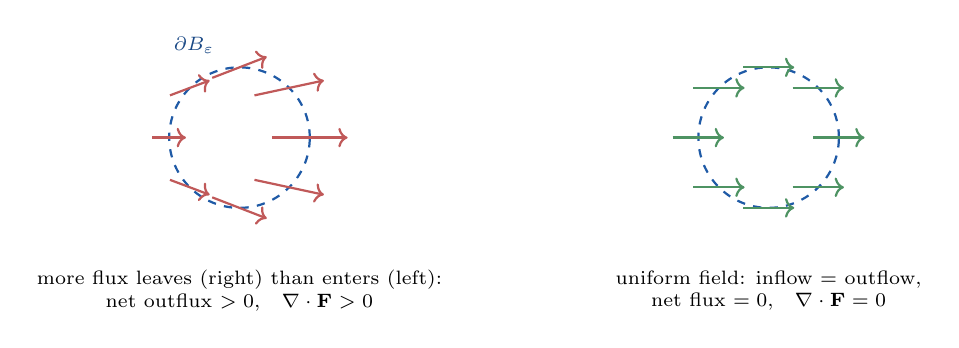
\begin{tikzpicture}[scale=1.05]
% ===== left panel: positive divergence (field F=(x,y) around P away from origin) =====
\begin{scope}
% test circle
\coordinate (P) at (0,0);
\draw[dashed, thick, figB] (P) circle (0.85);
% field F = (x,y) shifted: at points on circle centered at (2.2,0) global -> arrows grow rightward
% simulate: arrows at 8 circle points, vector = (2.2+cx, cy)*0.32
\foreach \ang in {0,45,90,135,180,225,270,315}{
  \pgfmathsetmacro{\cx}{0.85*cos(\ang)}
  \pgfmathsetmacro{\cy}{0.85*sin(\ang)}
  \pgfmathsetmacro{\fx}{(2.2+\cx)*0.30}
  \pgfmathsetmacro{\fy}{\cy*0.30}
  \draw[->, thick, figR!80] ({\cx-0.5*\fx},{\cy-0.5*\fy}) -- ({\cx+0.5*\fx},{\cy+0.5*\fy});
}
\node[font=\scriptsize, align=center] at (0,-1.85) {more flux leaves (right) than enters (left):\\ net outflux $> 0$, \; $\nabla\cdot\mathbf{F} > 0$};
\node[figB!80!black, font=\scriptsize] at (-0.55,1.12) {$\partial B_\varepsilon$};
\end{scope}
% ===== right panel: zero divergence (uniform field) =====
\begin{scope}[shift={(6.4,0)}]
\coordinate (P) at (0,0);
\draw[dashed, thick, figB] (P) circle (0.85);
\foreach \ang in {0,45,90,135,180,225,270,315}{
  \pgfmathsetmacro{\cx}{0.85*cos(\ang)}
  \pgfmathsetmacro{\cy}{0.85*sin(\ang)}
  \draw[->, thick, figG!80] ({\cx-0.31},\cy) -- ({\cx+0.31},\cy);
}
\node[font=\scriptsize, align=center] at (0,-1.85) {uniform field: inflow $=$ outflow,\\ net flux $= 0$, \; $\nabla\cdot\mathbf{F} = 0$};
\end{scope}
\end{tikzpicture}%
\figcap{Divergence is \textnormal{flux density}: $\nabla\cdot\mathbf{F}(P) = \lim_{\varepsilon\to 0} \frac{1}{|B_\varepsilon|}\oint_{\partial B_\varepsilon}\mathbf{F}\cdot\hat{n}\,ds$ --- shrink a test ball around $P$ and measure the net rate at which the field escapes, per unit area. Left: a stretching field pushes more flux out the far side than comes in the near side; the ball is a net source. Right: a uniform field passes straight through; whatever enters, leaves. The divergence theorem (\S18) is this local statement summed over a region: interior fluxes cancel (\S16), leaving the boundary flux.}
\end{center}

\subsection*{Curl (Vector $\to$ Vector, in $\R^3$ Only)}

For a vector field $\mathbf{F} = (F_1, F_2, F_3): \R^3 \to \R^3$, the \textbf{curl} is:
\[
\nabla \times \mathbf{F} = \left(\parti{F_3}{y} - \parti{F_2}{z}, \;\; \parti{F_1}{z} - \parti{F_3}{x}, \;\; \parti{F_2}{x} - \parti{F_1}{y}\right).
\]

This can be written mnemonically as a ``determinant'':
\[
\nabla \times \mathbf{F} = \begin{vmatrix} \hat{e}_x & \hat{e}_y & \hat{e}_z \\ \partial_x & \partial_y & \partial_z \\ F_1 & F_2 & F_3 \end{vmatrix}.
\]

Geometrically, $\nabla \times \mathbf{F}$ measures the \textit{local rotation} of the field. A field with $\nabla \times \mathbf{F} = \mathbf{0}$ everywhere is called \textit{irrotational} or \textit{curl-free}.

\begin{center}
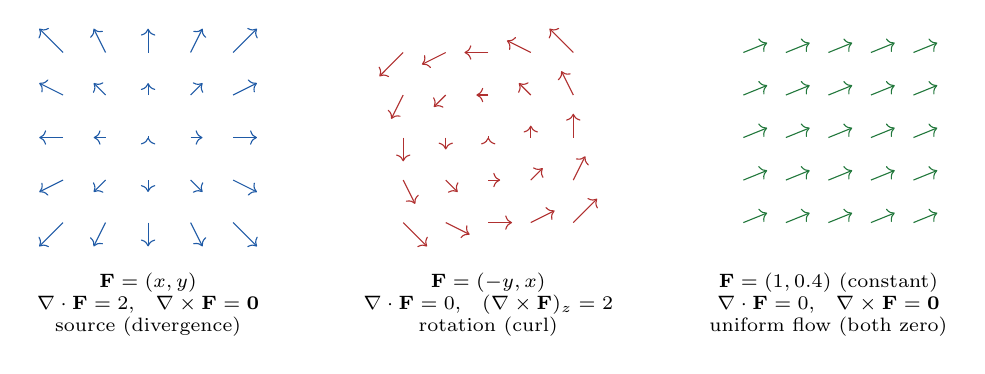
\begin{tikzpicture}[scale=0.72]
% Panel 1: gradient field of f = (x^2+y^2)/2, i.e. F = (x,y): radial outward, div = 2, curl = 0
\begin{scope}[shift={(0,0)}]
\foreach \x in {-1.5,-0.75,0,0.75,1.5}
  \foreach \y in {-1.5,-0.75,0,0.75,1.5}
    {\pgfmathsetmacro{\vx}{0.28*\x}
     \pgfmathsetmacro{\vy}{0.28*\y}
     \draw[->, figB, thin] (\x,\y) -- ({\x+\vx},{\y+\vy});}
\node[font=\scriptsize, align=center] at (0,-2.95) {$\mathbf{F} = (x, y)$\\ $\nabla \cdot \mathbf{F} = 2$, \; $\nabla \times \mathbf{F} = \mathbf{0}$\\ source (divergence)};
\end{scope}
% Panel 2: rotation field F = (-y,x): curl = 2, div = 0
\begin{scope}[shift={(6,0)}]
\foreach \x in {-1.5,-0.75,0,0.75,1.5}
  \foreach \y in {-1.5,-0.75,0,0.75,1.5}
    {\pgfmathsetmacro{\vx}{-0.28*\y}
     \pgfmathsetmacro{\vy}{0.28*\x}
     \draw[->, figR, thin] (\x,\y) -- ({\x+\vx},{\y+\vy});}
\node[font=\scriptsize, align=center] at (0,-2.95) {$\mathbf{F} = (-y, x)$\\ $\nabla \cdot \mathbf{F} = 0$, \; $(\nabla \times \mathbf{F})_z = 2$\\ rotation (curl)};
\end{scope}
% Panel 3: constant field F = (1, 0.4): div = 0, curl = 0
\begin{scope}[shift={(12,0)}]
\foreach \x in {-1.5,-0.75,0,0.75,1.5}
  \foreach \y in {-1.5,-0.75,0,0.75,1.5}
    \draw[->, figG, thin] (\x,\y) -- ({\x+0.42},{\y+0.17});
\node[font=\scriptsize, align=center] at (0,-2.95) {$\mathbf{F} = (1, 0.4)$ (constant)\\ $\nabla \cdot \mathbf{F} = 0$, \; $\nabla \times \mathbf{F} = \mathbf{0}$\\ uniform flow (both zero)};
\end{scope}
\end{tikzpicture}%
\figcap{Three vector fields illustrating the operators. Left: a radial source --- positive divergence, no rotation. Middle: rigid rotation --- positive curl, no spreading. Right: uniform flow --- neither. Divergence detects spreading; curl detects rotation.}
\end{center}

\begin{center}
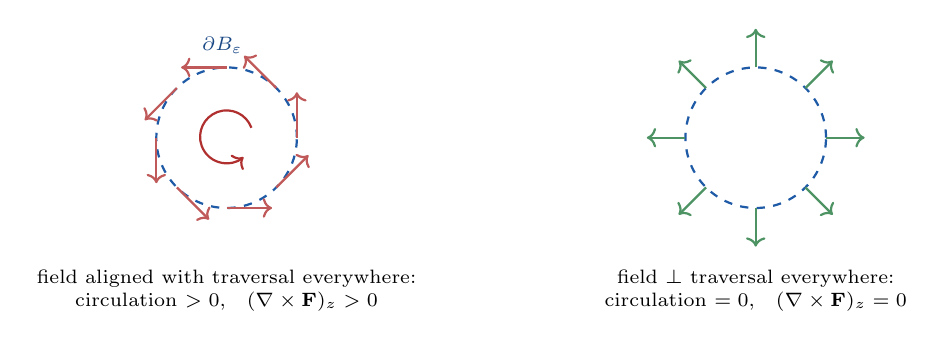
\begin{tikzpicture}[scale=1.05]
% ===== left panel: positive curl (rotational field F=(-y,x)) =====
\begin{scope}
\draw[dashed, thick, figB] (0,0) circle (0.85);
% field F = (-y,x) at circle points: tangential, ccw
\foreach \ang in {0,45,90,135,180,225,270,315}{
  \pgfmathsetmacro{\cx}{0.85*cos(\ang)}
  \pgfmathsetmacro{\cy}{0.85*sin(\ang)}
  \draw[->, thick, figR!80] (\cx,\cy) -- ({\cx-0.55*sin(\ang)},{\cy+0.55*cos(\ang)});
}
% paddle wheel hint: small ccw arc arrow at center
\draw[->, thick, figR] (0.3,0.12) arc[start angle=20, end angle=310, radius=0.32];
\node[font=\scriptsize, align=center] at (0,-1.85) {field aligned with traversal everywhere:\\ circulation $> 0$, \; $(\nabla\times\mathbf{F})_z > 0$};
\node[figB!80!black, font=\scriptsize] at (-0.05,1.12) {$\partial B_\varepsilon$};
\end{scope}
% ===== right panel: zero curl (radial field F=(x,y)) =====
\begin{scope}[shift={(6.4,0)}]
\draw[dashed, thick, figB] (0,0) circle (0.85);
\foreach \ang in {0,45,90,135,180,225,270,315}{
  \pgfmathsetmacro{\cx}{0.85*cos(\ang)}
  \pgfmathsetmacro{\cy}{0.85*sin(\ang)}
  \draw[->, thick, figG!80] (\cx,\cy) -- ({1.55*\cx},{1.55*\cy});
}
\node[font=\scriptsize, align=center] at (0,-1.85) {field $\perp$ traversal everywhere:\\ circulation $= 0$, \; $(\nabla\times\mathbf{F})_z = 0$};
\end{scope}
\end{tikzpicture}%
\figcap{Curl is \textnormal{circulation density}: $(\nabla\times\mathbf{F})_z(P) = \lim_{\varepsilon\to 0} \frac{1}{|B_\varepsilon|}\oint_{\partial B_\varepsilon}\mathbf{F}\cdot\mathbf{T}\,ds$ --- shrink a test loop around $P$ and measure how strongly the field pushes along it, per unit area (a paddle wheel placed at $P$ spins at this rate). Left: a rotational field drives the loop; positive curl. Right: a radial field is everywhere perpendicular to the loop; a paddle wheel would not turn --- zero curl, even though the field is far from constant. Stokes' theorem (\S20) is this local statement summed over a surface.}
\end{center}

\textbf{Why only $\R^3$?} The curl takes a vector field (3 components) and produces another vector field (3 components). This works because there are exactly 3 independent pairs from $\{x, y, z\}$: $(y,z)$, $(z,x)$, $(x,y)$. In $\R^2$, there is only 1 such pair, so the ``curl'' of a 2D field is a scalar, not a vector: $(\nabla \times \mathbf{F})_z = (F_2)_x - (F_1)_y$. In $\R^4$, there are 6 pairs, so the ``curl'' would have 6 components and cannot be a vector field. The exterior derivative (\S21) removes this dimension restriction.

\subsection*{Terminology for Vector Fields}

\begin{definition}[Conservative, Irrotational, Solenoidal]
A $C^1$ vector field $\mathbf{F}$ on a domain $D \subseteq \R^3$ is called:
\begin{itemize}
    \item \textbf{Conservative} (or a \textbf{gradient field}) if $\mathbf{F} = \nabla f$ for some scalar field $f$ (called the \textit{potential}).
    \item \textbf{Irrotational} (or \textbf{curl-free}) if $\nabla \times \mathbf{F} = \mathbf{0}$ everywhere on $D$.
    \item \textbf{Solenoidal} (or \textbf{divergence-free} or \textbf{incompressible}) if $\nabla \cdot \mathbf{F} = 0$ everywhere on $D$.
\end{itemize}
\end{definition}

\subsection*{Two Fundamental Identities}

For any $C^2$ scalar field $f$ and $C^2$ vector field $\mathbf{F}$ on $\R^3$:
\[
\nabla \times (\nabla f) = \mathbf{0} \qquad \text{and} \qquad \nabla \cdot (\nabla \times \mathbf{F}) = 0.
\]

In the terminology above: \textit{every conservative field is irrotational}, and \textit{every curl of a vector field is solenoidal}.

\textit{Proof of the first:} The $x$-component of $\nabla \times (\nabla f)$ is $f_{zy} - f_{yz} = 0$ by equality of mixed partials (\S5). The other components are similar.

\textit{Proof of the second:} $\nabla \cdot (\nabla \times \mathbf{F}) = (F_3)_{yx} - (F_2)_{zx} + (F_1)_{zy} - (F_3)_{xy} + (F_2)_{xz} - (F_1)_{yz} = 0$, again by equality of mixed partials.

The converses are more subtle: \textit{is every irrotational field conservative?} \textit{Is every solenoidal field a curl?} These depend on the \textit{topology} of the domain $D$. On all of $\R^3$ the answer is yes; on domains with holes (like $\R^3$ minus a line), it can fail. This will be made precise in Part III (\S22), where ``conservative'' becomes ``exact,'' ``irrotational'' becomes ``closed,'' and the failure of the converse is detected by de Rham cohomology.

These identities say: the image of one operator lies in the kernel of the next. In Part III (\S22), we will see that both are the \textit{same identity} $d^2 = 0$ applied at different levels, and that the equality of mixed partials (\S5) is the underlying reason for both.

\chapter{Existence Theorems and Applications}

\section{The Implicit Function Theorem}

\subsection*{Motivation: Curves Defined Implicitly}

Consider the equation $x^2 + y^2 = 1$ (a circle). This defines $y$ as a function of $x$ \textit{implicitly} --- we can solve to get $y = \pm\sqrt{1 - x^2}$, but only locally (we must choose a branch).

\begin{center}
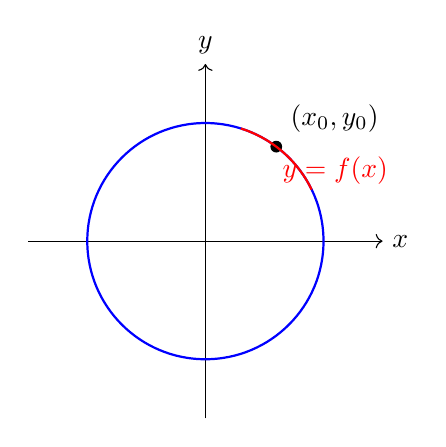
\begin{tikzpicture}[scale=1.5]
\draw[->] (-1.5,0) -- (1.5,0) node[right] {$x$};
\draw[->] (0,-1.5) -- (0,1.5) node[above] {$y$};
\draw[thick, blue] (0,0) circle (1);
\node[circle, fill, inner sep=1.5pt, label=above right:{$(x_0, y_0)$}] at (0.6, 0.8) {};
\draw[thick, red, domain=0.3:0.9] plot (\x, {sqrt(1-\x*\x)});
\node[red] at (1.1, 0.6) {$y = f(x)$};
\end{tikzpicture}
\end{center}

More generally, given $F(x, y) = 0$, when can we solve for $y = f(x)$ near a point $(x_0, y_0)$ on the curve?

\textbf{Key insight:} If $F(a, b) = 0$ and the curve is not ``horizontal'' at $(a, b)$ (i.e., $F_y(a, b) \neq 0$), then we can locally solve for $y$ as a function of $x$.

\subsection{Statement of the Theorem}

\begin{theorem}[Implicit Function Theorem]
Let $F : \R^2 \to \R$ satisfy the following conditions:
\begin{enumerate}[label=(\roman*)]
    \item $F(x_0, y_0) = 0$
    \item $F_y(x_0, y_0) \neq 0$
    \item $F_x$ and $F_y$ are continuous in a neighborhood $B((x_0, y_0); \varepsilon)$
\end{enumerate}

Then there exist $\delta > 0$ and a unique function $f : (x_0 - \delta, x_0 + \delta) \to \R$ such that:
\begin{enumerate}[label=(\alph*)]
    \item $f(x_0) = y_0$
    \item $F(x, f(x)) = 0$ for all $x \in (x_0 - \delta, x_0 + \delta)$
    \item $f$ is continuous on $(x_0 - \delta, x_0 + \delta)$
    \item $f$ is differentiable, with
    \[
    f'(x) = -\frac{F_x(x, f(x))}{F_y(x, f(x))}
    \]
\end{enumerate}
\end{theorem}

\subsection{Proof of the Implicit Function Theorem}

The proof proceeds in several steps: (1) establish existence of $f$, (2) prove uniqueness, (3) prove continuity, (4) prove differentiability.

\begin{proof}
Without loss of generality, assume $F_y(x_0, y_0) = a > 0$. (If $a < 0$, replace $F$ by $-F$.)

\textbf{Step 1: Setting up the neighborhood.}

Since $F_y$ is continuous at $(x_0, y_0)$ and $F_y(x_0, y_0) = a > 0$, there exists $\delta_1 > 0$ such that
\[
|x - x_0| < \delta_1 \text{ and } |y - y_0| < \delta_1 \implies F_y(x, y) > \frac{a}{2} > 0.
\]

This means $F$ is \textbf{strictly increasing in $y$} throughout the box $[x_0 - \delta_1, x_0 + \delta_1] \times [y_0 - \delta_1, y_0 + \delta_1]$.

\textbf{Step 2: Sign conditions on the boundary.}

Fix $x = x_0$. Since $F(x_0, \cdot)$ is strictly increasing in $y$ and $F(x_0, y_0) = 0$:
\[
F(x_0, y_0 + \delta_1) > F(x_0, y_0) = 0, \qquad F(x_0, y_0 - \delta_1) < F(x_0, y_0) = 0.
\]

Since $F$ is continuous (because $F_x, F_y$ exist and are continuous), there exists $\delta_2 > 0$ such that for all $x \in [x_0 - \delta_2, x_0 + \delta_2]$:
\[
F(x, y_0 + \delta_1) > 0, \qquad F(x, y_0 - \delta_1) < 0.
\]

(We apply continuity of $F$ at the two points $(x_0, y_0 + \delta_1)$ and $(x_0, y_0 - \delta_1)$, obtaining radii $\delta_2'$ and $\delta_2''$ respectively, then take $\delta_2 = \min\{\delta_2', \delta_2''\}$.)

\textbf{Step 3: Existence of $f(x)$ via the Intermediate Value Theorem.}

Let $\delta = \min\{\delta_1, \delta_2\}$. For each fixed $x \in [x_0 - \delta, x_0 + \delta]$:
\begin{itemize}[itemsep=2pt]
    \item The function $y \mapsto F(x, y)$ is continuous on $[y_0 - \delta_1, y_0 + \delta_1]$
    \item $F(x, y_0 - \delta_1) < 0$ and $F(x, y_0 + \delta_1) > 0$
\end{itemize}

By the Intermediate Value Theorem, there exists $y \in (y_0 - \delta_1, y_0 + \delta_1)$ such that $F(x, y) = 0$.

Define $f(x)$ to be this $y$-value.

\textbf{Step 4: Uniqueness of $f(x)$.}

Suppose there exist $y_1, y_2 \in (y_0 - \delta_1, y_0 + \delta_1)$ with $y_1 < y_2$ and $F(x, y_1) = F(x, y_2) = 0$.

Since $F_y(x, y) > \frac{a}{2} > 0$ throughout the box, $F(x, \cdot)$ is strictly increasing. But then $F(x, y_1) < F(x, y_2)$, contradicting $F(x, y_1) = F(x, y_2) = 0$.

Hence $f(x)$ is uniquely defined.

\textbf{Step 5: Continuity of $f$.}

We prove $f$ is continuous at $x_0$. (The proof at other points is identical.)

Let $\varepsilon > 0$ be given, with $\varepsilon < \delta_1$. We need to find $\delta > 0$ such that
\[
|x - x_0| < \delta \implies |f(x) - f(x_0)| < \varepsilon.
\]

We work within the rectangle $[x_0 - \delta, x_0 + \delta] \times [y_0 - \varepsilon, y_0 + \varepsilon]$, where $F_y > a/2 > 0$ (so $F$ is strictly increasing in $y$).

Since $F_y > \frac{a}{2}$ in the box, we have:
\[
F(x_0, y_0 + \varepsilon) \geq F(x_0, y_0) + \frac{a}{2} \cdot \varepsilon = \frac{a\varepsilon}{2} > 0.
\]

By continuity of $F$, there exists $\delta' > 0$ such that for $|x - x_0| < \delta'$:
\[
F(x, y_0 + \varepsilon) > 0, \qquad F(x, y_0 - \varepsilon) < 0.
\]

For such $x$, since $F(x, f(x)) = 0$ and $F(x, \cdot)$ is strictly increasing:
\[
F(x, y_0 - \varepsilon) < 0 = F(x, f(x)) < F(x, y_0 + \varepsilon).
\]

Therefore $y_0 - \varepsilon < f(x) < y_0 + \varepsilon$, i.e., $|f(x) - y_0| < \varepsilon$.

Since $f(x_0) = y_0$, we have $|f(x) - f(x_0)| < \varepsilon$ whenever $|x - x_0| < \delta'$.

Hence $f$ is continuous at $x_0$.

\textbf{Step 6: Differentiability of $f$ and the derivative formula.}

We need to show:
\[
\lim_{h \to 0} \frac{f(x_0 + h) - f(x_0)}{h} = -\frac{F_x(x_0, y_0)}{F_y(x_0, y_0)}.
\]

Since $F(x_0 + h, f(x_0 + h)) = 0$ and $F(x_0, f(x_0)) = 0$:
\[
0 = F(x_0 + h, f(x_0 + h)) - F(x_0, f(x_0)).
\]

Apply the Mean Value Theorem. Write:
\begin{align*}
0 &= F(x_0 + h, f(x_0 + h)) - F(x_0, f(x_0 + h)) + F(x_0, f(x_0 + h)) - F(x_0, f(x_0)) \\
&= F_x(x_0 + \alpha h, f(x_0 + h)) \cdot h + F_y(x_0, f(x_0) + \beta(f(x_0 + h) - f(x_0))) \cdot (f(x_0 + h) - f(x_0))
\end{align*}
for some $\alpha, \beta \in [0, 1]$.

Rearranging:
\[
\frac{f(x_0 + h) - f(x_0)}{h} = -\frac{F_x(x_0 + \alpha h, f(x_0 + h))}{F_y(x_0, f(x_0) + \beta(f(x_0 + h) - f(x_0)))}.
\]

As $h \to 0$:
\begin{itemize}[itemsep=2pt]
    \item $x_0 + \alpha h \to x_0$ (since $\alpha \in [0, 1]$)
    \item $f(x_0 + h) \to f(x_0) = y_0$ (by continuity of $f$, proved in Step 5)
    \item $f(x_0) + \beta(f(x_0 + h) - f(x_0)) \to y_0$ (since $\beta \in [0, 1]$ and $f(x_0 + h) \to y_0$)
\end{itemize}

By continuity of $F_x$ and $F_y$:
\[
\lim_{h \to 0} \frac{f(x_0 + h) - f(x_0)}{h} = -\frac{F_x(x_0, y_0)}{F_y(x_0, y_0)}.
\]

Hence $f$ is differentiable at $x_0$ with $f'(x_0) = -\dfrac{F_x(x_0, y_0)}{F_y(x_0, y_0)}$.

The same argument at any point $(x, f(x))$ in the domain gives:
\[
f'(x) = -\frac{F_x(x, f(x))}{F_y(x, f(x))}.
\]
\end{proof}

\subsection{Geometric Interpretation}

\begin{remark}[Why $F_y \neq 0$?]
The condition $F_y(x_0, y_0) \neq 0$ means the level curve $F(x, y) = 0$ is not horizontal at $(x_0, y_0)$.

If $F_y = 0$ but $F_x \neq 0$, the curve is vertical, and we should solve for $x$ as a function of $y$ instead.

If both $F_x = F_y = 0$, the point $(x_0, y_0)$ is a \textbf{singular point} of the curve, where the implicit function theorem does not apply.
\end{remark}

\begin{remark}[The Derivative Formula]
The formula $f'(x) = -\dfrac{F_x}{F_y}$ can be derived heuristically by implicit differentiation:

Starting from $F(x, f(x)) = 0$, differentiate both sides with respect to $x$:
\[
F_x(x, f(x)) \cdot 1 + F_y(x, f(x)) \cdot f'(x) = 0.
\]
Solving for $f'(x)$:
\[
f'(x) = -\frac{F_x(x, f(x))}{F_y(x, f(x))}.
\]

The Implicit Function Theorem justifies this formal computation by proving $f$ exists and is differentiable.
\end{remark}

\begin{example}[Circle]
Let $F(x, y) = x^2 + y^2 - 1$. Then $F_x = 2x$ and $F_y = 2y$.

At $(x_0, y_0) = (0, 1)$: $F(0, 1) = 0$, $F_y(0, 1) = 2 \neq 0$.

By the Implicit Function Theorem, near $(0, 1)$ we can solve for $y = f(x)$, and:
\[
f'(x) = -\frac{F_x}{F_y} = -\frac{2x}{2y} = -\frac{x}{y}.
\]

Indeed, $f(x) = \sqrt{1 - x^2}$ near $(0, 1)$, and $f'(x) = \dfrac{-x}{\sqrt{1 - x^2}} = -\dfrac{x}{f(x)}$. \checkmark
\end{example}

\begin{example}[Where IFT Fails]
Consider $F(x, y) = x^2 + y^2 - 1$ at the point $(1, 0)$.

Here $F_y(1, 0) = 0$, so the Implicit Function Theorem does not apply.

Indeed, near $(1, 0)$, the circle is vertical --- we cannot express $y$ as a single-valued function of $x$.

However, $F_x(1, 0) = 2 \neq 0$, so we can solve for $x$ as a function of $y$ near this point.
\end{example}

\subsection*{Summary of the Proof Structure}

\begin{center}
\begin{tabular}{|c|l|l|}
\hline
\textbf{Step} & \textbf{Goal} & \textbf{Key Tool} \\
\hline
1 & Set up neighborhood where $F_y > 0$ & Continuity of $F_y$ \\
\hline
2 & Sign conditions: $F > 0$ on top, $F < 0$ on bottom & Continuity of $F$ \\
\hline
3 & Existence of $f(x)$ & Intermediate Value Theorem \\
\hline
4 & Uniqueness of $f(x)$ & Strict monotonicity ($F_y > 0$) \\
\hline
5 & Continuity of $f$ & $\varepsilon$-$\delta$ using monotonicity \\
\hline
6 & Differentiability of $f$ & MVT + continuity of $F_x, F_y$ \\
\hline
\end{tabular}
\end{center}

\subsection{Implicit Function Theorem: Multivariable Case}

The Implicit Function Theorem generalizes to functions of more variables.

\begin{theorem}[Implicit Function Theorem --- General Case]
Let $F(x_1, x_2, \ldots, x_n, y)$ satisfy:
\begin{enumerate}[label=(\roman*)]
    \item $F(x_1^{(0)}, x_2^{(0)}, \ldots, x_n^{(0)}, y^{(0)}) = 0$
    \item $F_y(x_1^{(0)}, x_2^{(0)}, \ldots, x_n^{(0)}, y^{(0)}) \neq 0$
    \item All partial derivatives $F_{x_1}, \ldots, F_{x_n}, F_y$ are continuous in a neighborhood of $(x^{(0)}, y^{(0)})$
\end{enumerate}

Then there exists a function $y = Y(x_1, \ldots, x_n)$ defined in a neighborhood of $(x_1^{(0)}, \ldots, x_n^{(0)})$ such that:
\begin{enumerate}[label=(\alph*)]
    \item $F(x_1, \ldots, x_n, Y(x_1, \ldots, x_n)) = 0$
    \item $Y$ is continuously differentiable with
    \[
    \frac{\partial Y}{\partial x_i} = -\frac{F_{x_i}(x, Y(x))}{F_y(x, Y(x))}
    \]
\end{enumerate}
\end{theorem}

\begin{remark}
The proof follows the same structure as the two-variable case. The condition $F_y \neq 0$ ensures we can solve for $y$ in terms of the other variables.
\end{remark}

\begin{center}
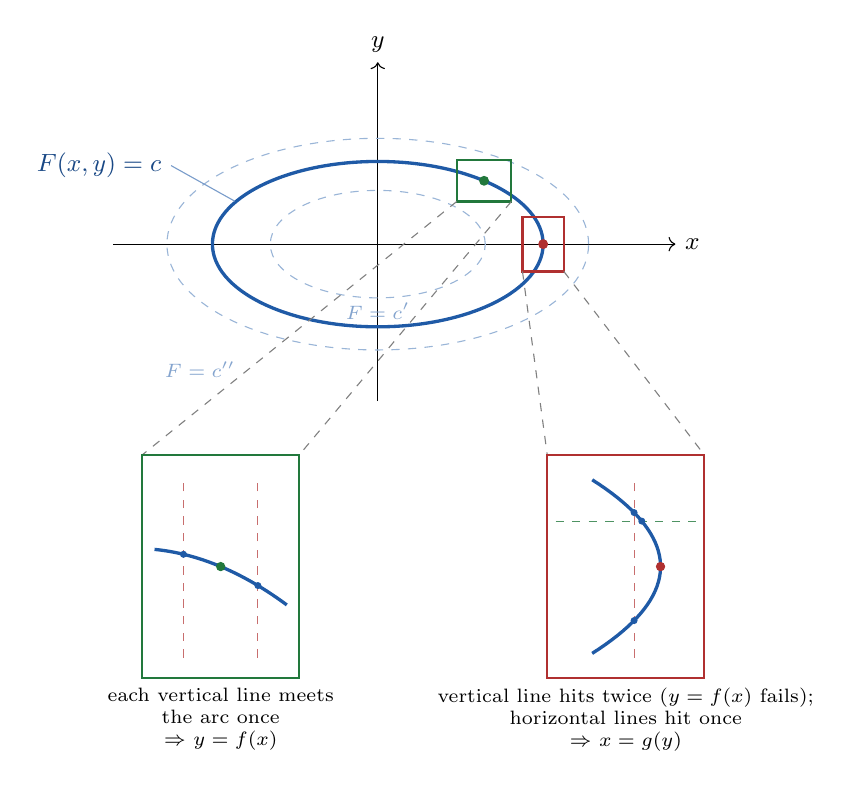
\begin{tikzpicture}[scale=1.05]
% ====== main panel: contour map of F = x^2/4 + y^2 ======
\draw[->] (-3.2,0) -- (3.6,0) node[right, font=\small] {$x$};
\draw[->] (0,-1.9) -- (0,2.2) node[above, font=\small] {$y$};
% neighboring contours (dashed)
\draw[dashed, figB!45] (0,0) ellipse (1.30 and 0.65);
\draw[dashed, figB!45] (0,0) ellipse (2.55 and 1.28);
\node[figB!55, font=\scriptsize] at (0,-0.81) {$F=c'$};
\node[figB!55, font=\scriptsize] at (-2.15,-1.52) {$F=c''$};
% the contour of interest (solid)
\draw[very thick, figB] (0,0) ellipse (2.0 and 1.0);
\node[figB!80!black, font=\small, anchor=east] (clab) at (-2.5,0.95) {$F(x,y)=c$};
\draw[figB!60, thin] (clab.east) -- (-1.73,0.52);
% --- point (a): generic point at t=50deg ---
\coordinate (Pa) at ({2*cos(50)},{sin(50)});
\filldraw[figG] (Pa) circle (1.5pt);
\draw[figG, thick] ($(Pa)+(-0.33,-0.25)$) rectangle ($(Pa)+(0.33,0.25)$);
% --- point (b): rightmost point (2,0), vertical tangent ---
\coordinate (Pb) at (2,0);
\filldraw[figR] (Pb) circle (1.5pt);
\draw[figR, thick] ($(Pb)+(-0.25,-0.33)$) rectangle ($(Pb)+(0.25,0.33)$);
% ====== zoom leader lines ======
\draw[dashed, gray] ($(Pa)+(-0.33,-0.25)$) -- (-2.85,-2.55);
\draw[dashed, gray] ($(Pa)+(0.33,-0.25)$) -- (-0.95,-2.55);
\draw[dashed, gray] ($(Pb)+(-0.25,-0.33)$) -- (2.05,-2.55);
\draw[dashed, gray] ($(Pb)+(0.25,-0.33)$) -- (3.95,-2.55);
% ====== zoom A: generic point, graph over x ======
\begin{scope}[shift={(-1.9,-3.9)}]
\draw[figG, thick] (-0.95,-1.35) rectangle (0.95,1.35);
% magnified arc near t=50: y = sqrt(1-x^2/4) recentered; locally like a line with slope dy/dx=-x/(4y)=-0.42
\draw[very thick, figB, domain=-0.8:0.8, samples=40] plot (\x, {-0.42*\x - 0.20*\x*\x});
\filldraw[figG] (0,0) circle (1.4pt);
% vertical line test: two dashed verticals, each one intersection
\draw[dashed, figR!70] (-0.45,-1.1) -- (-0.45,1.1);
\draw[dashed, figR!70] (0.45,-1.1) -- (0.45,1.1);
\filldraw[figB] (-0.45,{0.42*0.45 - 0.20*0.2025}) circle (1.0pt);
\filldraw[figB] (0.45,{-0.42*0.45 - 0.20*0.2025}) circle (1.0pt);
\node[font=\scriptsize, align=center] at (0,-1.85) {each vertical line meets\\ the arc once\\ $\Rightarrow$ $y=f(x)$};
\end{scope}
% ====== zoom B: vertical tangent, graph over y only ======
\begin{scope}[shift={(3.0,-3.9)}]
\draw[figR, thick] (-0.95,-1.35) rectangle (0.95,1.35);
% magnified arc near (2,0): x = 2 sqrt(1-y^2) ~ 2 - y^2 recentered: left-opening parabola x = -y^2 (scaled)
\draw[very thick, figB, domain=-1.05:1.05, samples=40, variable=\y] plot ({-0.75*\y*\y+0.42}, \y);
\filldraw[figR] (0.42,0) circle (1.4pt);
% vertical line: hits twice
\draw[dashed, figR!70] (0.10,-1.1) -- (0.10,1.1);
\filldraw[figB] (0.10,{sqrt(0.32/0.75)}) circle (1.0pt);
\filldraw[figB] (0.10,{-sqrt(0.32/0.75)}) circle (1.0pt);
% horizontal line: hits once
\draw[dashed, figG!80] (-0.85,0.55) -- (0.85,0.55);
\filldraw[figB] ({-0.75*0.3025+0.42},0.55) circle (1.0pt);
\node[font=\scriptsize, align=center] at (0,-1.85) {vertical line hits twice ($y=f(x)$ fails);\\ horizontal lines hit once\\ $\Rightarrow$ $x=g(y)$};
\end{scope}
\end{tikzpicture}%
\figcap{The Implicit Function Theorem on a contour map of the paraboloid $F = x^2/4 + y^2$ (dashed: neighboring levels; solid: the contour $F = c$). Zooming in at a generic point (green), the arc passes the vertical line test: locally $y = f(x)$, possible because $F_y \neq 0$ there. Zooming in at the rightmost point (red), the tangent is vertical ($F_y = 2y = 0$): the arc fails the vertical line test, and no $y = f(x)$ exists --- but $F_x \neq 0$, the arc passes the \textnormal{horizontal} line test, and $x = g(y)$ works. A regular contour is always locally a graph; the gradient tells you over which axis.}
\end{center}

\section{The Inverse Function Theorem}

\subsection*{Motivation: Inverting Functions}

\textbf{One dimension:} If $y = h(x)$ and $h'(x_0) \neq 0$, then $h$ is locally invertible near $x_0$, and:
\[
(h^{-1})'(y_0) = \frac{1}{h'(x_0)} = \frac{1}{h'(h^{-1}(y_0))}.
\]

\textbf{Two dimensions:} Given a mapping $(x, y) \mapsto (u, v)$ where $u = \varphi(x, y)$ and $v = \psi(x, y)$, when can we invert to get $x = f(u, v)$ and $y = g(u, v)$?

\subsection*{The Key Question: What Do We Want?}

\textbf{What we have:} A mapping $(x, y) \mapsto (u, v)$ where $u = \varphi(x,y)$ and $v = \psi(x,y)$.

\textbf{What we want:}
\begin{enumerate}[itemsep=2pt]
    \item Does an inverse mapping $(u, v) \mapsto (x, y)$ exist locally?
    \item If so, what are the partial derivatives $f_u, f_v, g_u, g_v$ of the inverse?
\end{enumerate}

\textbf{The problem:} We generally \textbf{cannot write down explicit formulas} for $f$ and $g$!

\begin{example}[Why Explicit Inversion is Hard]
Given $u = x^2 - y^2$ and $v = 2xy$, try solving for $x$ and $y$ in terms of $u$ and $v$. 

You would need to solve a system of nonlinear equations --- very difficult in general!
\end{example}

\textbf{What the Inverse Function Theorem gives us:}

Even though we can't find $f$ and $g$ explicitly, we get:
\begin{enumerate}[itemsep=2pt]
    \item \textbf{Existence:} If $\det(J) \neq 0$, then $f$ and $g$ \textbf{exist} locally (even if we can't write them down).
    \item \textbf{Derivatives:} We can compute the partial derivatives of $f$ and $g$ \textbf{without knowing the explicit formulas}:
    \[
    \begin{pmatrix} f_u & f_v \\ g_u & g_v \end{pmatrix} = \begin{pmatrix} \varphi_x & \varphi_y \\ \psi_x & \psi_y \end{pmatrix}^{-1}.
    \]
\end{enumerate}

\textbf{Why is this useful?} In many applications, we only need the derivatives, not the explicit inverse:
\begin{itemize}[itemsep=2pt]
    \item In change of variables for integration, we need $|\det(J)|$
    \item In differential equations, we need how variables transform locally
    \item In optimization, we need to understand local behavior
\end{itemize}

\subsection{The Jacobian Matrix}

\begin{definition}[Jacobian Matrix]
For a mapping $(x, y) \mapsto (\varphi(x,y), \psi(x,y))$, the \textbf{Jacobian matrix} is:
\[
J = \frac{\partial(\varphi, \psi)}{\partial(x, y)} = \begin{pmatrix} \varphi_x & \varphi_y \\ \psi_x & \psi_y \end{pmatrix}.
\]
\end{definition}

\textbf{What does the Jacobian do?} It describes how the mapping behaves \textbf{locally} near a point. If we make a small displacement $(dx, dy)$ in the input, the output changes by approximately:
\[
\begin{pmatrix} du \\ dv \end{pmatrix} \approx \begin{pmatrix} \varphi_x & \varphi_y \\ \psi_x & \psi_y \end{pmatrix} \begin{pmatrix} dx \\ dy \end{pmatrix} = J \begin{pmatrix} dx \\ dy \end{pmatrix}.
\]

In other words: \textbf{the Jacobian is the linear approximation to the mapping near a point}.

\textbf{When is the mapping invertible?} For the inverse to exist locally, we need to recover $(dx, dy)$ from $(du, dv)$:
\[
\begin{pmatrix} dx \\ dy \end{pmatrix} = J^{-1} \begin{pmatrix} du \\ dv \end{pmatrix}.
\]

This requires $J$ to be an \textbf{invertible matrix}, i.e., $\det(J) \neq 0$.

\subsection*{How to Invert a $2 \times 2$ Matrix}

\begin{proposition}[Inverse of a $2 \times 2$ Matrix]
If $A = \begin{pmatrix} a & b \\ c & d \end{pmatrix}$ and $\det(A) = ad - bc \neq 0$, then:
\[
A^{-1} = \frac{1}{ad - bc} \begin{pmatrix} d & -b \\ -c & a \end{pmatrix}.
\]
\end{proposition}

\begin{proof}
Direct verification:
\[
\begin{pmatrix} a & b \\ c & d \end{pmatrix} \cdot \frac{1}{ad-bc} \begin{pmatrix} d & -b \\ -c & a \end{pmatrix} = \frac{1}{ad-bc} \begin{pmatrix} ad - bc & 0 \\ 0 & ad - bc \end{pmatrix} = \begin{pmatrix} 1 & 0 \\ 0 & 1 \end{pmatrix}.
\]
\end{proof}

\begin{remark}[Recipe for $2 \times 2$ Inverse]
To invert $\begin{pmatrix} a & b \\ c & d \end{pmatrix}$:
\begin{enumerate}[itemsep=2pt]
    \item Swap the diagonal entries: $a \leftrightarrow d$
    \item Negate the off-diagonal entries: $b \to -b$, $c \to -c$
    \item Divide by the determinant $ad - bc$
\end{enumerate}
\end{remark}

\textbf{Applying to the Jacobian:}
\[
\begin{pmatrix} \varphi_x & \varphi_y \\ \psi_x & \psi_y \end{pmatrix}^{-1} = \frac{1}{\varphi_x \psi_y - \varphi_y \psi_x} \begin{pmatrix} \psi_y & -\varphi_y \\ -\psi_x & \varphi_x \end{pmatrix}.
\]

\subsection{Statement of the Theorem}

\begin{theorem}[Inverse Function Theorem]
Let $\varphi, \psi : \R^2 \to \R$ have continuous partial derivatives in a neighborhood of $(x_0, y_0)$. Define the Jacobian:
\[
J = \begin{pmatrix} \varphi_x & \varphi_y \\ \psi_x & \psi_y \end{pmatrix}.
\]

If $\det(J) \neq 0$ at $(x_0, y_0)$, then the mapping $(x, y) \mapsto (\varphi(x,y), \psi(x,y))$ is locally invertible near $(x_0, y_0)$.

That is, there exist functions $f, g$ such that locally:
\[
x = f(\varphi(x,y), \psi(x,y)), \qquad y = g(\varphi(x,y), \psi(x,y)),
\]
and the Jacobian of the inverse is:
\[
\begin{pmatrix} f_u & f_v \\ g_u & g_v \end{pmatrix} = J^{-1} = \frac{1}{\det(J)} \begin{pmatrix} \psi_y & -\varphi_y \\ -\psi_x & \varphi_x \end{pmatrix}.
\]
\end{theorem}

\begin{proof}[Proof via the Implicit Function Theorem]
The strategy is to apply the Implicit Function Theorem \textbf{twice} to ``peel off'' the variables one at a time: first solve for $x$, then solve for $y$.

\textbf{Setup and notation.} We have $u = \varphi(x,y)$ and $v = \psi(x,y)$, and we want to solve for $x$ and $y$ in terms of $u$ and $v$.

The key difficulty: in the equation $\varphi(x,y) = u$, the variable $u$ \textbf{depends on} $(x,y)$. We cannot directly apply IFT because we need the ``target'' to be an independent parameter. To fix this, introduce \textbf{free parameters} $\tilde{u}, \tilde{v}$ that are independent of everything, and solve:
\[
F(x, y, \tilde{u}) \equiv \varphi(x, y) - \tilde{u} = 0, \qquad G(x, y, \tilde{v}) \equiv \psi(x, y) - \tilde{v} = 0.
\]

Define $u_0 = \varphi(x_0, y_0)$ and $v_0 = \psi(x_0, y_0)$. Then $F(x_0, y_0, u_0) = 0$ and $G(x_0, y_0, v_0) = 0$.

\textbf{Variable dependence at start:} $x, y, \tilde{u}, \tilde{v}$ are all independent.

\medskip
\textbf{Step 1: Solve $F = 0$ for $x$.}

WLOG assume $\varphi_x(x_0, y_0) \neq 0$. (Since $\det(J) = \varphi_x \psi_y - \varphi_y \psi_x \neq 0$, at least one of $\varphi_x, \psi_x$ is nonzero; if $\varphi_x = 0$, relabel.)

We have:
\[
F(x, y, \tilde{u}) = \varphi(x, y) - \tilde{u} = 0, \qquad F_x = \varphi_x \neq 0.
\]

By the Implicit Function Theorem (applied to $F = 0$, solving for $x$ in terms of $y, \tilde{u}$):

There exists a function $x = X(y, \tilde{u})$ defined near $(y_0, u_0)$ such that:
\begin{enumerate}[label=(\roman*), itemsep=2pt]
    \item $X(y_0, u_0) = x_0$
    \item $F(X(y, \tilde{u}), y, \tilde{u}) = 0$, i.e., $\varphi(X(y, \tilde{u}), y) = \tilde{u}$
    \item $X_y = -\dfrac{F_y}{F_x} = -\dfrac{\varphi_y(X(y,\tilde{u}), y)}{\varphi_x(X(y,\tilde{u}), y)}$
\end{enumerate}

\textbf{Variable dependence after Step 1:} $y, \tilde{u}, \tilde{v}$ are independent; $x = X(y, \tilde{u})$ depends on $y, \tilde{u}$.

\medskip
\textbf{Step 2: Substitute into $G = 0$ and solve for $y$.}

Plug $x = X(y, \tilde{u})$ into the second equation:
\[
H(y, \tilde{u}, \tilde{v}) \equiv G(X(y, \tilde{u}), y, \tilde{v}) = \psi(X(y, \tilde{u}), y) - \tilde{v} = 0.
\]

We need $H_y \neq 0$ to apply IFT. Compute using the chain rule:
\begin{align*}
H_y &= \psi_x(X(y,\tilde{u}), y) \cdot X_y(y, \tilde{u}) + \psi_y(X(y,\tilde{u}), y) \\[4pt]
&= \psi_x \cdot \left( -\frac{\varphi_y}{\varphi_x} \right) + \psi_y \\[4pt]
&= \frac{-\psi_x \varphi_y + \psi_y \varphi_x}{\varphi_x} \\[4pt]
&= \frac{1}{\varphi_x} \begin{vmatrix} \varphi_x & \varphi_y \\ \psi_x & \psi_y \end{vmatrix} = \frac{\det(J)}{\varphi_x}.
\end{align*}

Since $\det(J) \neq 0$ and $\varphi_x \neq 0$, we have $H_y \neq 0$. Also $H(y_0, u_0, v_0) = G(x_0, y_0, v_0) = 0$.

By the Implicit Function Theorem (applied to $H = 0$, solving for $y$ in terms of $\tilde{u}, \tilde{v}$):

There exists a function $y = Y(\tilde{u}, \tilde{v})$ defined near $(u_0, v_0)$ such that:
\begin{enumerate}[label=(\roman*), itemsep=2pt]
    \item $Y(u_0, v_0) = y_0$
    \item $H(Y(\tilde{u}, \tilde{v}), \tilde{u}, \tilde{v}) = 0$, i.e., $\psi(X(Y(\tilde{u},\tilde{v}), \tilde{u}), Y(\tilde{u}, \tilde{v})) = \tilde{v}$
\end{enumerate}

\textbf{Variable dependence after Step 2:} $\tilde{u}, \tilde{v}$ are independent; $y = Y(\tilde{u}, \tilde{v})$ and $x = X(Y(\tilde{u}, \tilde{v}), \tilde{u})$ both depend on $\tilde{u}, \tilde{v}$.

\medskip
\textbf{Step 3: Define the inverse functions.}

Set:
\[
f(\tilde{u}, \tilde{v}) \equiv X(Y(\tilde{u}, \tilde{v}), \tilde{u}), \qquad g(\tilde{u}, \tilde{v}) \equiv Y(\tilde{u}, \tilde{v}).
\]

\textbf{Variable dependence at end:} $\tilde{u}, \tilde{v}$ are independent; $x = f(\tilde{u}, \tilde{v})$ and $y = g(\tilde{u}, \tilde{v})$ depend on them. The roles of $(x,y)$ and $(u,v)$ are now \textbf{reversed}.

\medskip
\textbf{Step 4: Verify the inverse property.}

From Step 1: $\varphi(X(y, \tilde{u}), y) = \tilde{u}$ for all $(y, \tilde{u})$ near $(y_0, u_0)$.

Setting $y = Y(\tilde{u}, \tilde{v}) = g(\tilde{u}, \tilde{v})$ and $X(Y(\tilde{u}, \tilde{v}), \tilde{u}) = f(\tilde{u}, \tilde{v})$:
\[
\varphi(f(\tilde{u}, \tilde{v}), g(\tilde{u}, \tilde{v})) = \tilde{u}. \quad \checkmark
\]

From Step 2: $\psi(X(Y(\tilde{u}, \tilde{v}), \tilde{u}), Y(\tilde{u}, \tilde{v})) = \tilde{v}$, i.e.:
\[
\psi(f(\tilde{u}, \tilde{v}), g(\tilde{u}, \tilde{v})) = \tilde{v}. \quad \checkmark
\]

Since $\tilde{u}, \tilde{v}$ were free parameters playing the role of $u, v$, we drop the tildes and conclude: $f(u, v)$ and $g(u, v)$ are the desired inverse functions.
\end{proof}

\begin{remark}[Tracking Variable Dependencies]
The proof works by progressively ``solving away'' the original variables:
\begin{center}
\begin{tabular}{|c|l|l|}
\hline
\textbf{Stage} & \textbf{Independent variables} & \textbf{Dependent variables} \\
\hline
Start & $x, y, \tilde{u}, \tilde{v}$ & --- \\
\hline
After Step 1 & $y, \tilde{u}, \tilde{v}$ & $x = X(y, \tilde{u})$ \\
\hline
After Step 2 & $\tilde{u}, \tilde{v}$ & $y = Y(\tilde{u}, \tilde{v})$, \; $x = X(Y(\tilde{u},\tilde{v}), \tilde{u})$ \\
\hline
\end{tabular}
\end{center}
\end{remark}

\begin{remark}[Why $\tilde{u}, \tilde{v}$ Are Needed]
In the original setup, $u = \varphi(x,y)$ depends on $(x,y)$. The Implicit Function Theorem requires solving an equation like $\varphi(x,y) = c$ where $c$ is a \textbf{free parameter} independent of the variables being solved for. By introducing $\tilde{u}$ as an independent copy of $u$, we create a legitimate IFT setup. At the end, the inverse satisfies $\varphi(f(u,v), g(u,v)) = u$, so setting $\tilde{u} = u$ is justified.
\end{remark}

\begin{remark}[Tracking IFT Hypotheses]
\begin{center}
\begin{tabular}{|c|l|l|l|l|}
\hline
\textbf{Step} & \textbf{Equation} & \textbf{Solve for} & \textbf{IFT condition} & \textbf{Why satisfied} \\
\hline
1 & $\varphi(x,y) - \tilde{u} = 0$ & $x = X(y, \tilde{u})$ & $F_x = \varphi_x \neq 0$ & WLOG \\
\hline
2 & $\psi(X(y,\tilde{u}),y) - \tilde{v} = 0$ & $y = Y(\tilde{u}, \tilde{v})$ & $H_y = \dfrac{\det J}{\varphi_x} \neq 0$ & $\det J \neq 0$, $\varphi_x \neq 0$ \\[6pt]
\hline
\end{tabular}
\end{center}
\end{remark}

\begin{remark}[Comparison: 1D vs 2D]
\begin{center}
\begin{tabular}{|c|c|c|}
\hline
& \textbf{1D} & \textbf{2D} \\
\hline
Forward & $u = \varphi(x)$ & $(u, v) = (\varphi(x,y), \psi(x,y))$ \\
\hline
Inverse & $x = \varphi^{-1}(u)$ & $(x, y) = (f(u, v), g(u, v))$ \\
\hline
Condition & $\varphi'(x) \neq 0$ & $\det(J) \neq 0$ \\
\hline
Derivative of inverse & $(\varphi^{-1})' = \dfrac{1}{\varphi'}$ & $D(f, g) = J^{-1}$ \\
\hline
\end{tabular}
\end{center}
\end{remark}

\subsection{Derivation via Chain Rule}

We now derive the formula $D(f, g) = J^{-1}$ using the chain rule.

Suppose the inverse exists: $x = f(u, v)$, $y = g(u, v)$.

Then the composition gives the identity:
\[
(x, y) = (f(\varphi(x,y), \psi(x,y)), \, g(\varphi(x,y), \psi(x,y))).
\]

\textbf{Using the chain rule:} For $f(u, v)$ where $u = \varphi(x,y)$ and $v = \psi(x,y)$:
\[
\begin{pmatrix} \partial_x f \\ \partial_y f \end{pmatrix} = \begin{pmatrix} f_u u_x + f_v v_x \\ f_u u_y + f_v v_y \end{pmatrix} = \begin{pmatrix} u_x & v_x \\ u_y & v_y \end{pmatrix} \begin{pmatrix} f_u \\ f_v \end{pmatrix}.
\]

Similarly for $g(u, v)$:
\[
\begin{pmatrix} \partial_x g \\ \partial_y g \end{pmatrix} = \begin{pmatrix} u_x & v_x \\ u_y & v_y \end{pmatrix} \begin{pmatrix} g_u \\ g_v \end{pmatrix}.
\]

\textbf{Combining into matrix form:}
\[
\begin{pmatrix} \partial_x f & \partial_x g \\ \partial_y f & \partial_y g \end{pmatrix} = \begin{pmatrix} \varphi_x & \psi_x \\ \varphi_y & \psi_y \end{pmatrix} \begin{pmatrix} f_u & g_u \\ f_v & g_v \end{pmatrix}.
\]

\textbf{Applying to the identity:} Since $f(\varphi(x,y), \psi(x,y)) = x$ and $g(\varphi(x,y), \psi(x,y)) = y$:
\[
\begin{pmatrix} \partial_x f & \partial_x g \\ \partial_y f & \partial_y g \end{pmatrix} = \begin{pmatrix} 1 & 0 \\ 0 & 1 \end{pmatrix}.
\]

Substituting:
\[
\begin{pmatrix} 1 & 0 \\ 0 & 1 \end{pmatrix} = \begin{pmatrix} \varphi_x & \psi_x \\ \varphi_y & \psi_y \end{pmatrix} \begin{pmatrix} f_u & g_u \\ f_v & g_v \end{pmatrix}.
\]

\textbf{Solving for the inverse Jacobian:}
\[
\begin{pmatrix} f_u & g_u \\ f_v & g_v \end{pmatrix} = \begin{pmatrix} \varphi_x & \psi_x \\ \varphi_y & \psi_y \end{pmatrix}^{-1}.
\]

Taking the transpose:
\[
\boxed{\begin{pmatrix} f_u & f_v \\ g_u & g_v \end{pmatrix} = \begin{pmatrix} \varphi_x & \varphi_y \\ \psi_x & \psi_y \end{pmatrix}^{-1} = J^{-1}}
\]

\subsection*{Example: Finding Derivatives of the Inverse}

\begin{example}
Consider the mapping:
\[
u = \varphi(x, y) = x^2 - y^2, \qquad v = \psi(x, y) = 2xy.
\]

Suppose the inverse exists: $x = f(u, v)$, $y = g(u, v)$. Find $f_u, f_v, g_u, g_v$.

\textbf{Step 1: Compute the Jacobian.}
\[
J = \begin{pmatrix} \varphi_x & \varphi_y \\ \psi_x & \psi_y \end{pmatrix} = \begin{pmatrix} 2x & -2y \\ 2y & 2x \end{pmatrix}.
\]

\textbf{Step 2: Check invertibility.}
\[
\det(J) = 4x^2 + 4y^2 = 4(x^2 + y^2) \neq 0 \quad \text{for } (x, y) \neq (0, 0).
\]

\textbf{Step 3: Compute $J^{-1}$.}
\[
J^{-1} = \frac{1}{4(x^2 + y^2)} \begin{pmatrix} 2x & 2y \\ -2y & 2x \end{pmatrix} = \frac{1}{2(x^2 + y^2)} \begin{pmatrix} x & y \\ -y & x \end{pmatrix}.
\]

\textbf{Step 4: Read off the partial derivatives.}
\[
f_u = \frac{x}{2(x^2 + y^2)}, \quad f_v = \frac{y}{2(x^2 + y^2)}, \quad g_u = \frac{-y}{2(x^2 + y^2)}, \quad g_v = \frac{x}{2(x^2 + y^2)}.
\]

\textbf{Note:} The formulas are in terms of $(x, y)$, but $f, g$ are functions of $(u, v)$. To express purely in $(u, v)$, we would substitute $x = f(u, v)$, $y = g(u, v)$ --- but we don't know those explicitly!

\textbf{The power of the theorem:} We found the derivatives without explicit formulas for $f$ and $g$.
\end{example}

\begin{center}
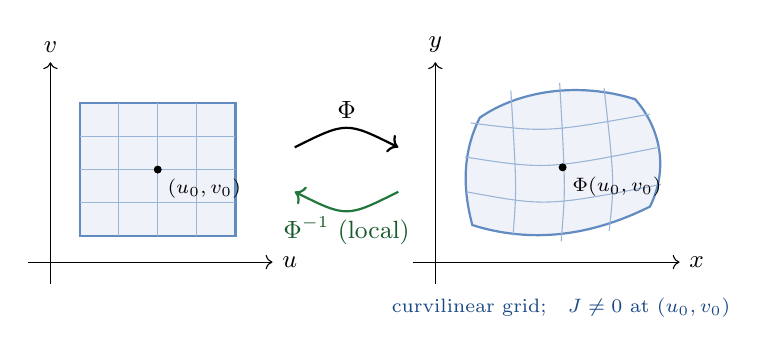
\begin{tikzpicture}[scale=0.94]
% left: (u,v) grid
\begin{scope}
\draw[->] (-0.3,0) -- (3.0,0) node[right, font=\small] {$u$};
\draw[->] (0,-0.3) -- (0,2.7) node[above, font=\small] {$v$};
\draw[thick, figB!70, fill=figB!7] (0.4,0.35) rectangle (2.5,2.15);
\foreach \u in {0.925,1.45,1.975} \draw[figB!45, thin] (\u,0.35) -- (\u,2.15);
\foreach \v in {0.8,1.25,1.7} \draw[figB!45, thin] (0.4,\v) -- (2.5,\v);
\filldraw (1.45,1.25) circle (1.3pt);
\node[font=\scriptsize, below right] at (1.45,1.25) {$(u_0,v_0)$};
\end{scope}
% forward and inverse arrows
\draw[->, thick] (3.3,1.55) .. controls (4.0,1.9) .. (4.7,1.55);
\node[font=\small] at (4.0,2.05) {$\Phi$};
\draw[<-, thick, figG] (3.3,0.95) .. controls (4.0,0.6) .. (4.7,0.95);
\node[figG!75!black, font=\small] at (4.0,0.42) {$\Phi^{-1}$ (local)};
% right: curvilinear image grid
\begin{scope}[shift={(5.2,0)}]
\draw[->] (-0.3,0) -- (3.3,0) node[right, font=\small] {$x$};
\draw[->] (0,-0.3) -- (0,2.7) node[above, font=\small] {$y$};
\draw[thick, figB!70, fill=figB!7]
  (0.5,0.5) .. controls (1.3,0.25) and (2.1,0.35) .. (2.9,0.75)
  .. controls (3.15,1.25) and (3.05,1.8) .. (2.7,2.2)
  .. controls (1.9,2.45) and (1.1,2.3) .. (0.6,1.95)
  .. controls (0.35,1.45) and (0.38,0.95) .. (0.5,0.5) -- cycle;
\draw[figB!45, thin] (1.05,0.36) .. controls (1.1,1.0) .. (1.02,2.32);
\draw[figB!45, thin] (1.7,0.28) .. controls (1.76,1.0) .. (1.68,2.42);
\draw[figB!45, thin] (2.35,0.42) .. controls (2.42,1.1) .. (2.28,2.35);
\draw[figB!45, thin] (0.42,0.95) .. controls (1.5,0.75) .. (3.05,1.05);
\draw[figB!45, thin] (0.40,1.42) .. controls (1.5,1.25) .. (3.02,1.55);
\draw[figB!45, thin] (0.48,1.88) .. controls (1.5,1.75) .. (2.9,2.0);
\filldraw (1.72,1.28) circle (1.3pt);
\node[font=\scriptsize, below right] at (1.72,1.28) {$\Phi(u_0,v_0)$};
\node[font=\scriptsize, figB!80!black, align=center] at (1.7,-0.62) {curvilinear grid; \; $J \neq 0$ at $(u_0,v_0)$};
\end{scope}
\end{tikzpicture}%
\figcap{The Inverse Function Theorem as a mapping statement: if $J = \det D\Phi \neq 0$ at a point, the map takes the flat grid to a curvilinear grid that is locally one-to-one --- grid lines cross transversally, so each image point has a unique preimage nearby, and a local $C^1$ inverse exists. Where $J = 0$ the grid degenerates (cells collapse) and invertibility can fail.}
\end{center}

\subsection*{Example: Polar Coordinates}

\begin{example}[Cartesian to Polar]
Define $r = r(x, y) = \sqrt{x^2 + y^2}$ and $\theta = \theta(x, y) = \arctan(y/x)$.

The partial derivatives are:
\[
r_x = \frac{x}{r}, \quad r_y = \frac{y}{r}, \quad \theta_x = -\frac{y}{r^2}, \quad \theta_y = \frac{x}{r^2}.
\]

The Jacobian matrix and determinant:
\[
J = \begin{pmatrix} x/r & y/r \\ -y/r^2 & x/r^2 \end{pmatrix}, \qquad |J| = \frac{x^2 + y^2}{r^3} = \frac{1}{r}.
\]
\end{example}

\begin{example}[Polar to Cartesian]
Define $x = r\cos\theta$ and $y = r\sin\theta$.

The Jacobian matrix and determinant:
\[
J = \begin{pmatrix} \cos\theta & -r\sin\theta \\ \sin\theta & r\cos\theta \end{pmatrix}, \qquad |J| = r.
\]
\end{example}

\begin{remark}[Reciprocal Jacobians]
The Jacobian determinants are reciprocals: $\dfrac{1}{r} \cdot r = 1$.

This is a general fact: if two mappings are inverses, their Jacobian determinants are reciprocals.
\end{remark}

% ================================================================================
\section{Optimization and Lagrange Multipliers}
% ================================================================================

\subsection{Unconstrained Optimization}

\begin{definition}[Local Maximum/Minimum]
A function $f(x, y)$ has a \textbf{local maximum} at $(x_0, y_0)$ if there exists $\delta > 0$ such that $f(x, y) \leq f(x_0, y_0)$ for all $(x, y)$ with $\|(x, y) - (x_0, y_0)\| < \delta$.

Similarly for \textbf{local minimum} with $f(x, y) \geq f(x_0, y_0)$.
\end{definition}

\begin{theorem}[Necessary Condition for Extremum --- Fermat's Theorem in $\R^n$]
If $f$ has a local max/min at $(x_0, y_0)$ and $f$ is differentiable there, then
\[
f_x(x_0, y_0) = 0 \quad \text{and} \quad f_y(x_0, y_0) = 0.
\]
Equivalently, $\nabla f(x_0, y_0) = \mathbf{0}$.
\end{theorem}

\begin{proof}
Consider the single-variable function $g(x) = f(x, y_0)$ obtained by fixing $y = y_0$. If $f$ has a local max at $(x_0, y_0)$, then $g$ has a local max at $x_0$.

By Fermat's theorem from single-variable calculus (451), $g'(x_0) = 0$.

But $g'(x) = f_x(x, y_0)$, so $f_x(x_0, y_0) = 0$.

By the same argument with $h(y) = f(x_0, y)$, we get $f_y(x_0, y_0) = 0$.
\end{proof}

\begin{remark}
A point where $\nabla f = \mathbf{0}$ is called a \textbf{critical point} or \textbf{stationary point}. Not every critical point is a max or min --- it could be a saddle point.
\end{remark}

\subsection*{Constrained Optimization: The Setup}

Now suppose we want to optimize $f(x, y)$ subject to a constraint $g(x, y) = 0$.

\begin{example}
Maximize $f(x, y) = xy$ subject to $g(x, y) = x^2 + y^2 - 1 = 0$ (on the unit circle).
\end{example}

The constraint $g(x, y) = 0$ defines a curve in $\R^2$. We seek points on this curve where $f$ is maximized or minimized.

\subsection*{Geometric Insight: Tangent and Normal Vectors}

Suppose the constraint curve $g(x, y) = 0$ can be parametrized as $(x(t), y(t))$. Along this curve:
\[
g(x(t), y(t)) = 0 \quad \text{for all } t.
\]

Differentiating with respect to $t$:
\[
\frac{d}{dt}[g(x(t), y(t))] = g_x \cdot x'(t) + g_y \cdot y'(t) = \nabla g \cdot (x'(t), y'(t)) = 0.
\]

This shows: $\nabla g \perp (x'(t), y'(t))$, i.e., \textbf{$\nabla g$ is perpendicular to the tangent vector of the constraint curve}.

In other words, $\nabla g$ is \textbf{normal} (perpendicular) to the level curve $g = 0$.

\subsection{Derivation of the Lagrange Condition}

Now consider $F(t) = f(x(t), y(t))$, the value of $f$ along the constraint curve.

If $f$ has a max/min at $t = t_0$ along the curve, then $F'(t_0) = 0$ (by Fermat's theorem).

By the chain rule:
\[
F'(t_0) = f_x \cdot x'(t_0) + f_y \cdot y'(t_0) = \nabla f \cdot (x'(t_0), y'(t_0)) = 0.
\]

This shows: $\nabla f \perp (x'(t_0), y'(t_0))$, i.e., \textbf{$\nabla f$ is also perpendicular to the tangent vector}.

\textbf{Key conclusion:} At a constrained extremum, both $\nabla f$ and $\nabla g$ are perpendicular to the same tangent vector.

In $\R^2$, there is essentially only one direction perpendicular to the tangent. Therefore:
\[
\boxed{\nabla f \parallel \nabla g \quad \Longleftrightarrow \quad \nabla f = \lambda \nabla g \text{ for some } \lambda \in \R.}
\]

\begin{center}
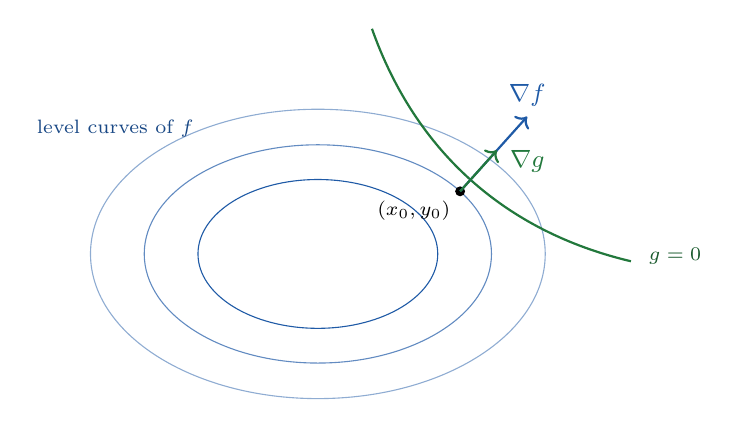
\begin{tikzpicture}[scale=1.05]
% level curves of f: nested ellipses centered at (0.3, 0.2)
\draw[figB!50] (0.3,0.2) ellipse (2.75 and 1.75);
\draw[figB!70] (0.3,0.2) ellipse (2.1 and 1.32);
\draw[figB] (0.3,0.2) ellipse (1.45 and 0.9);
\node[figB!80!black, font=\scriptsize] at (-2.15,1.72) {level curves of $f$};
% constraint curve g=0: a smooth curve tangent to middle ellipse at point P
% middle ellipse (2.1, 1.32) at angle t=35deg:
\coordinate (P) at ({0.3+2.1*cos(35)},{0.2+1.32*sin(35)});
% tangent dir of ellipse: (-a sin t, b cos t)
\coordinate (Tv) at ({-2.1*sin(35)},{1.32*cos(35)});
% draw g=0 as a curve through P along the tangent, gently bending away
\draw[thick, figG] ($(P)+1.3*(Tv)+(0.5,0.56)$) .. controls ($(P)+0.45*(Tv)$) and ($(P)-0.45*(Tv)$) .. ($(P)-1.3*(Tv)+(0.5,0.56)$);
\node[figG!75!black, font=\scriptsize, anchor=west] at ($(P)-1.3*(Tv)+(0.6,0.62)$) {$g = 0$};
% tangency point
\filldraw (P) circle (1.5pt) node[below left, font=\scriptsize] {$(x_0,y_0)$};
% gradient of f (outward normal to ellipse): (b cos t, a sin t) direction
\coordinate (Nf) at ({1.32*cos(35)*0.75},{2.1*sin(35)*0.75});
\draw[->, thick, figB] (P) -- ($(P)+(Nf)$) node[above, font=\small] {$\nabla f$};
% gradient of g: parallel, shorter
\draw[->, thick, figG] (P) -- ($(P)+0.55*(Nf)$) node[right=1pt, font=\small, yshift=-4pt] {$\nabla g$};
\end{tikzpicture}%
\figcap{At a constrained extremum, the constraint curve $g = 0$ is tangent to a level curve of $f$: crossing a level curve would mean $f$ still changes along the constraint. Tangency forces the two normals $\nabla f$ and $\nabla g$ to be parallel --- the Lagrange condition.}
\end{center}

\begin{theorem}[Method of Lagrange Multipliers]
Let $f, g: \R^2 \to \R$ be $C^1$ functions. Suppose $f$ has a local max/min at $(x_0, y_0)$ subject to the constraint $g(x_0, y_0) = 0$.

If $\nabla g(x_0, y_0) \neq \mathbf{0}$ (the \textbf{constraint qualification}), then there exists $\lambda \in \R$ such that:
\[
\nabla f(x_0, y_0) = \lambda \nabla g(x_0, y_0).
\]
Equivalently:
\[
f_x = \lambda g_x, \quad f_y = \lambda g_y, \quad g(x, y) = 0.
\]
\end{theorem}

\begin{proof}
We give a proof using the Implicit Function Theorem.

Since $\nabla g(x_0, y_0) \neq \mathbf{0}$, at least one of $g_x$ or $g_y$ is nonzero. WLOG, assume $g_y(x_0, y_0) \neq 0$.

By IFT, there exists a $C^1$ function $\alpha(x)$ defined near $x_0$ such that:
\[
g(x, \alpha(x)) = 0 \quad \text{and} \quad \alpha(x_0) = y_0.
\]
Moreover, $\alpha'(x) = -\dfrac{g_x}{g_y}$.

Now $f$ restricted to the constraint curve becomes a single-variable function:
\[
F(x) = f(x, \alpha(x)).
\]

If $f$ has a max/min at $(x_0, y_0)$ on the constraint, then $F$ has a max/min at $x_0$.

By Fermat's theorem: $F'(x_0) = 0$.

Computing $F'$ by the chain rule:
\[
F'(x) = f_x(x, \alpha(x)) + f_y(x, \alpha(x)) \cdot \alpha'(x) = f_x - f_y \cdot \frac{g_x}{g_y}.
\]

Setting $F'(x_0) = 0$:
\[
f_x - f_y \cdot \frac{g_x}{g_y} = 0 \quad \Longrightarrow \quad f_x g_y = f_y g_x \quad \Longrightarrow \quad \frac{f_x}{g_x} = \frac{f_y}{g_y} = \lambda.
\]

Therefore $f_x = \lambda g_x$ and $f_y = \lambda g_y$, i.e., $\nabla f = \lambda \nabla g$.
\end{proof}

\begin{remark}[The Constraint Qualification]
The condition $\nabla g \neq \mathbf{0}$ is essential. If $\nabla g = \mathbf{0}$ at a point on the constraint curve, that point is called a \textbf{singular point} of the constraint. The IFT does not apply there, and the Lagrange multiplier method may fail.

Geometrically, $\nabla g = \mathbf{0}$ means the constraint curve may have a cusp, self-intersection, or isolated point --- it's not a smooth curve locally.
\end{remark}

\begin{remark}[What if $f_y = 0$?]
In the proof, we assumed $g_y \neq 0$. What if $g_y \neq 0$ but $f_y = 0$?

From the equation $f_x = \lambda g_x$ and $f_y = \lambda g_y$ with $f_y = 0$ and $g_y \neq 0$, we get $\lambda = 0$.

Then $f_x = 0 \cdot g_x = 0$ as well. So $\nabla f = \mathbf{0}$, which is consistent with $\nabla f = \lambda \nabla g = \mathbf{0}$.

The Lagrange equations still hold, just with $\lambda = 0$. This corresponds to a ``free'' critical point where the constraint happens to pass through a critical point of $f$.
\end{remark}

\subsection{Higher Dimensions: Multiple Constraints}

\begin{theorem}[Lagrange Multipliers with Multiple Constraints]
To optimize $f(x_1, \ldots, x_n)$ subject to constraints $g_1 = 0, g_2 = 0, \ldots, g_k = 0$ (where $k < n$):

If the gradients $\nabla g_1, \ldots, \nabla g_k$ are linearly independent at a constrained extremum, then there exist $\lambda_1, \ldots, \lambda_k \in \R$ such that:
\[
\nabla f = \lambda_1 \nabla g_1 + \lambda_2 \nabla g_2 + \cdots + \lambda_k \nabla g_k.
\]
\end{theorem}

\begin{remark}[Why Multiple Constraints?]
In $\R^3$, a single constraint $g(x, y, z) = 0$ defines a surface (2D object). To get a curve (1D object), we need two constraints.

Geometrically: $\nabla g_1$ and $\nabla g_2$ are both normal to the constraint curve. The tangent to the curve is perpendicular to both. At a constrained extremum, $\nabla f$ must also be perpendicular to the tangent, so $\nabla f$ lies in the plane spanned by $\nabla g_1$ and $\nabla g_2$.

This is why we need $\nabla f = \lambda_1 \nabla g_1 + \lambda_2 \nabla g_2$ rather than just $\nabla f = \lambda \nabla g$.

In $\R^2$, two vectors perpendicular to the same vector must be parallel. In $\R^3$ and higher, two vectors perpendicular to the same vector need only lie in a plane --- they are not necessarily parallel!
\end{remark}

\subsection*{Practical Method: Solving Lagrange Equations}

To find candidates for constrained extrema of $f$ subject to $g = 0$:

\textbf{Step 1:} Write down the system of equations:
\begin{align*}
f_x &= \lambda g_x \\
f_y &= \lambda g_y \\
g(x, y) &= 0
\end{align*}

\textbf{Step 2:} Solve this system for $x$, $y$, and $\lambda$. (Three equations, three unknowns.)

\textbf{Step 3:} Evaluate $f$ at each solution to determine which gives the max/min.

\begin{remark}
The Lagrange conditions are \textbf{necessary} but not sufficient. They find all \emph{candidates} for extrema. To determine if a candidate is actually a max, min, or neither, we must either:
\begin{itemize}
    \item Compare values of $f$ at all candidates (if the constraint set is compact, EVT guarantees max/min exist).
    \item Use the bordered Hessian (second-order test for constrained optimization).
\end{itemize}
\end{remark}

\subsection*{Worked Example: $f = xy$ on the Unit Circle}

\begin{example}
Maximize and minimize $f(x, y) = xy$ subject to $\phi(x, y) = x^2 + y^2 - 1 = 0$.
\end{example}

\textbf{Step 1: Set up the Lagrange equations.}

The key condition is $\nabla f \parallel \nabla \phi$, i.e., $\nabla f = \lambda \nabla \phi$.
\begin{align*}
f_x &= \lambda \phi_x \quad \Rightarrow \quad y = \lambda \cdot 2x = 2\lambda x \tag{1} \\
f_y &= \lambda \phi_y \quad \Rightarrow \quad x = \lambda \cdot 2y = 2\lambda y \tag{2} \\
\phi(x,y) &= 0 \quad \Rightarrow \quad x^2 + y^2 = 1 \tag{3}
\end{align*}

\textbf{Step 2: Solve the system.}

From (1): $y = 2\lambda x$. Substitute into (2):
\[
x = 2\lambda y = 2\lambda(2\lambda x) = 4\lambda^2 x
\]
So $x(1 - 4\lambda^2) = 0$. Either $x = 0$ or $\lambda^2 = \frac{1}{4}$, i.e., $\lambda = \pm\frac{1}{2}$.

\textbf{Case 1:} $x = 0$. From (3): $y^2 = 1$, so $y = \pm 1$. From (1): $y = 2\lambda \cdot 0 = 0$, contradiction. So $x = 0$ gives no solutions.

\textbf{Case 2:} $\lambda = \frac{1}{2}$. From (1): $y = 2 \cdot \frac{1}{2} \cdot x = x$. From (3): $x^2 + x^2 = 1$, so $x = \pm\frac{1}{\sqrt{2}}$, $y = \pm\frac{1}{\sqrt{2}}$ (same sign).

Solutions: $\left(\frac{1}{\sqrt{2}}, \frac{1}{\sqrt{2}}\right)$ and $\left(-\frac{1}{\sqrt{2}}, -\frac{1}{\sqrt{2}}\right)$.

\textbf{Case 3:} $\lambda = -\frac{1}{2}$. From (1): $y = -x$. From (3): $x^2 + x^2 = 1$, so $x = \pm\frac{1}{\sqrt{2}}$, $y = \mp\frac{1}{\sqrt{2}}$ (opposite signs).

Solutions: $\left(\frac{1}{\sqrt{2}}, -\frac{1}{\sqrt{2}}\right)$ and $\left(-\frac{1}{\sqrt{2}}, \frac{1}{\sqrt{2}}\right)$.

\textbf{Step 3: Evaluate $f$ at each candidate.}
\begin{align*}
f\left(\frac{1}{\sqrt{2}}, \frac{1}{\sqrt{2}}\right) &= \frac{1}{2} \quad \text{(maximum)} \\
f\left(-\frac{1}{\sqrt{2}}, -\frac{1}{\sqrt{2}}\right) &= \frac{1}{2} \quad \text{(maximum)} \\
f\left(\frac{1}{\sqrt{2}}, -\frac{1}{\sqrt{2}}\right) &= -\frac{1}{2} \quad \text{(minimum)} \\
f\left(-\frac{1}{\sqrt{2}}, \frac{1}{\sqrt{2}}\right) &= -\frac{1}{2} \quad \text{(minimum)}
\end{align*}

\subsection{General Case: Two Constraints in $\R^4$}

Consider optimizing $f(x, y, z, t)$ subject to two constraints:
\[
\phi(x, y, z, t) = 0, \qquad \psi(x, y, z, t) = 0.
\]

The constraint set is generically a 2-dimensional surface in $\R^4$.

\textbf{Constraint qualification:} The gradients $\nabla \phi$ and $\nabla \psi$ are linearly independent. Equivalently, the $2 \times 4$ Jacobian matrix has rank 2, meaning some $2 \times 2$ submatrix has nonzero determinant.

Suppose 
\[
\det \begin{pmatrix} \phi_z & \phi_t \\ \psi_z & \psi_t \end{pmatrix} \neq 0.
\]

By IFT, we can locally solve for $z = g(x, y)$ and $t = h(x, y)$ such that:
\[
\phi(x, y, g(x,y), h(x,y)) = 0, \qquad \psi(x, y, g(x,y), h(x,y)) = 0.
\]

\begin{remark}[Notation Convention]
Once we substitute $z = g(x,y)$ and $t = h(x,y)$, we write:
\begin{itemize}
    \item $\phi_g$ for the partial derivative of $\phi$ with respect to its third argument (the slot filled by $g$), i.e., $\phi_g = \phi_z$ evaluated at $(x, y, g, h)$.
    \item $\phi_h$ for the partial derivative of $\phi$ with respect to its fourth argument (the slot filled by $h$), i.e., $\phi_h = \phi_t$ evaluated at $(x, y, g, h)$.
\end{itemize}
Similarly for $\psi_g, \psi_h$ and $f_g, f_h$. This notation reminds us that these arguments are now functions of $(x, y)$, not independent variables.
\end{remark}

With this notation, the constraint qualification becomes:
\[
\det \begin{pmatrix} \phi_g & \phi_h \\ \psi_g & \psi_h \end{pmatrix} \neq 0.
\]

\textbf{Reduced problem:} Optimize $F(x, y) = f(x, y, g(x,y), h(x,y))$ (unconstrained in two variables).

At an extremum $(x_0, y_0)$:
\[
\frac{\partial F}{\partial x} = 0, \qquad \frac{\partial F}{\partial y} = 0.
\]

\textbf{Computing the derivatives:} By chain rule,
\begin{align*}
\frac{\partial F}{\partial x} &= f_x + f_g \cdot g_x + f_h \cdot h_x = 0 \\
\frac{\partial F}{\partial y} &= f_y + f_g \cdot g_y + f_h \cdot h_y = 0
\end{align*}

In matrix form:
\[
(f_g, f_h) \begin{pmatrix} g_x & g_y \\ h_x & h_y \end{pmatrix} = -(f_x, f_y) \tag{$*$}
\]

\textbf{Finding $g_x, g_y, h_x, h_y$:} Differentiate the constraints.

From $\phi(x, y, g, h) = 0$:
\begin{align*}
\phi_x + \phi_g \cdot g_x + \phi_h \cdot h_x &= 0 \\
\phi_y + \phi_g \cdot g_y + \phi_h \cdot h_y &= 0
\end{align*}

From $\psi(x, y, g, h) = 0$:
\begin{align*}
\psi_x + \psi_g \cdot g_x + \psi_h \cdot h_x &= 0 \\
\psi_y + \psi_g \cdot g_y + \psi_h \cdot h_y &= 0
\end{align*}

In matrix form:
\[
\begin{pmatrix} \phi_g & \phi_h \\ \psi_g & \psi_h \end{pmatrix} \begin{pmatrix} g_x & g_y \\ h_x & h_y \end{pmatrix} = -\begin{pmatrix} \phi_x & \phi_y \\ \psi_x & \psi_y \end{pmatrix} \tag{$**$}
\]

\textbf{Combining the equations:} Substituting $(**)$ into $(*)$:
\[
(f_g, f_h) \begin{pmatrix} g_x & g_y \\ h_x & h_y \end{pmatrix} = -(f_x, f_y)
\]

Let $A = \begin{pmatrix} \phi_g & \phi_h \\ \psi_g & \psi_h \end{pmatrix}$. From $(**)$: 
\[
\begin{pmatrix} g_x & g_y \\ h_x & h_y \end{pmatrix} = -A^{-1} \begin{pmatrix} \phi_x & \phi_y \\ \psi_x & \psi_y \end{pmatrix}
\]

So $(*)$ becomes:
\[
-(f_g, f_h) A^{-1} \begin{pmatrix} \phi_x & \phi_y \\ \psi_x & \psi_y \end{pmatrix} = -(f_x, f_y)
\]

\textbf{Define Lagrange multipliers:} Let $(\lambda, \mu) = (f_g, f_h) A^{-1}$, i.e.,
\[
(f_g, f_h) = (\lambda, \mu) A = (\lambda, \mu) \begin{pmatrix} \phi_g & \phi_h \\ \psi_g & \psi_h \end{pmatrix} = (\lambda \phi_g + \mu \psi_g, \lambda \phi_h + \mu \psi_h)
\]

This gives:
\[
f_g = \lambda \phi_g + \mu \psi_g, \qquad f_h = \lambda \phi_h + \mu \psi_h \tag{I}
\]

Or in terms of the original variables:
\[
f_z = \lambda \phi_z + \mu \psi_z, \qquad f_t = \lambda \phi_t + \mu \psi_t
\]

\textbf{Verify the equations for $x$ and $y$:} From the manipulation above:
\[
(\lambda, \mu) \begin{pmatrix} \phi_x & \phi_y \\ \psi_x & \psi_y \end{pmatrix} = (f_x, f_y)
\]

This gives:
\[
f_x = \lambda \phi_x + \mu \psi_x, \qquad f_y = \lambda \phi_y + \mu \psi_y \tag{II}
\]

\textbf{Conclusion:} Combining (I) and (II), at a constrained extremum $(x_0, y_0, z_0, t_0)$:
\[
\boxed{\nabla f = \lambda \nabla \phi + \mu \nabla \psi}
\]

Together with the constraints $\phi = 0$ and $\psi = 0$, this gives 6 equations in 6 unknowns $(x, y, z, t, \lambda, \mu)$.

\begin{remark}[Choice of Variables for IFT]
We assumed $\det \begin{pmatrix} \phi_g & \phi_h \\ \psi_g & \psi_h \end{pmatrix} \neq 0$ and solved for $(z, t)$ as functions $g(x,y), h(x,y)$ of the free variables $(x, y)$.

We could equally well have used any other $2 \times 2$ submatrix with nonzero determinant. For instance, if $\det \begin{pmatrix} \phi_y & \phi_h \\ \psi_y & \psi_h \end{pmatrix} \neq 0$, we could solve for $(y, t)$ as functions of $(x, z)$.

The final Lagrange equations $\nabla f = \lambda \nabla \phi + \mu \nabla \psi$ are \textbf{independent of this choice}. This is the key insight: the multipliers $\lambda, \mu$ adjust to give the same geometric condition regardless of how we parametrize the constraint surface.
\end{remark}

\subsection{Second-Order Sufficient Conditions: The Hessian Test}

The Lagrange conditions $\nabla f = \mathbf{0}$ (unconstrained) or $\nabla f = \lambda \nabla g$ (constrained) are \textbf{necessary} for an extremum, but not sufficient. A critical point could be a max, min, or saddle point. The Hessian test provides \textbf{sufficient} conditions.

\begin{definition}[Hessian Matrix]
For $f \in C^2$ near $(x_0, y_0)$, the \textbf{Hessian matrix} is:
\[
H = \begin{pmatrix} f_{xx} & f_{xy} \\ f_{yx} & f_{yy} \end{pmatrix}
\]
evaluated at $(x_0, y_0)$. By Schwarz--Clairaut, $H$ is symmetric: $f_{xy} = f_{yx}$.
\end{definition}

\begin{remark}[The Hessian as the Second Total Derivative]
Just as the gradient $\nabla f$ is the first total derivative --- a linear map $Df_{\mathbf{p}}: \mathbf{v} \mapsto \nabla f \cdot \mathbf{v}$ that captures the first-order behavior of $f$ (\S6--\S8) --- the Hessian is the \textit{second} total derivative: a bilinear form $D^2f_{\mathbf{p}}: (\mathbf{u}, \mathbf{v}) \mapsto \mathbf{u}^T H_f \mathbf{v}$ that captures the second-order behavior. The Taylor expansion from \S9 says exactly this (where $\mathbf{p} \in \R^n$ is the base point and $\mathbf{h} \in \R^n$ is the increment):
\[
f(\mathbf{p} + \mathbf{h}) = f(\mathbf{p}) + \underbrace{Df_{\mathbf{p}}(\mathbf{h})}_{\text{linear: gradient}} + \frac{1}{2}\underbrace{D^2f_{\mathbf{p}}(\mathbf{h}, \mathbf{h})}_{\text{bilinear: Hessian}} + o(|\mathbf{h}|^2).
\]

The positive/negative definiteness test below asks: is this bilinear form positive for all directions $\mathbf{h}$? The symmetry of $H$ ($f_{xy} = f_{yx}$) will reappear in a deeper role when we study differential forms (\S22).
\end{remark}

\begin{definition}[Positive/Negative Definite]
A symmetric matrix $A = \begin{pmatrix} a & b \\ b & c \end{pmatrix}$ is:
\begin{itemize}
    \item \textbf{Positive definite} if $\mathbf{x}^T A \mathbf{x} > 0$ for all $\mathbf{x} \neq \mathbf{0}$.
    \item \textbf{Negative definite} if $\mathbf{x}^T A \mathbf{x} < 0$ for all $\mathbf{x} \neq \mathbf{0}$.
    \item \textbf{Indefinite} if $\mathbf{x}^T A \mathbf{x}$ takes both positive and negative values.
\end{itemize}

Explicitly, for $\mathbf{x} = (h, k)^T$:
\[
\mathbf{x}^T A \mathbf{x} = (h, k) \begin{pmatrix} a & b \\ b & c \end{pmatrix} \begin{pmatrix} h \\ k \end{pmatrix} = (h, k) \begin{pmatrix} ah + bk \\ bh + ck \end{pmatrix} = ah^2 + 2bhk + ck^2.
\]
\end{definition}

\begin{theorem}[Second-Order Sufficient Conditions --- Unconstrained]
Let $f \in C^2(B_\varepsilon(x_0, y_0))$ with $f_x(x_0, y_0) = f_y(x_0, y_0) = 0$ (critical point).

Let $H = \begin{pmatrix} f_{xx} & f_{xy} \\ f_{xy} & f_{yy} \end{pmatrix}$ be the Hessian at $(x_0, y_0)$.

\begin{enumerate}
    \item If $H$ is positive definite, then $f$ has a \textbf{local minimum} at $(x_0, y_0)$.
    \item If $H$ is negative definite, then $f$ has a \textbf{local maximum} at $(x_0, y_0)$.
    \item If $H$ is indefinite, then $(x_0, y_0)$ is a \textbf{saddle point}.
\end{enumerate}
\end{theorem}

\begin{center}
\includegraphics[width=0.98\textwidth]{pyfigs/f20_critical_points.pdf}%
\figcap{The three nondegenerate critical point types, classified by the Hessian: both eigenvalues positive (bowl, local min), both negative (dome, local max), mixed signs (saddle). The second derivative test of \S14 reads these signs from $f_{xx}$ and $\det H = f_{xx}f_{yy} - f_{xy}^2$.}
\end{center}


\begin{proof}[Proof sketch]
By Taylor's theorem (single-variable version applied to $F(t) = f(x_0 + th, y_0 + tk)$):
\[
f(x_0 + h, y_0 + k) = f(x_0, y_0) + \underbrace{f_x h + f_y k}_{= 0} + \frac{1}{2}\left( f_{xx} h^2 + 2f_{xy} hk + f_{yy} k^2 \right)\Big|_{(x_0 + \theta h, y_0 + \theta k)}
\]
for some $\theta \in (0, 1)$.

Using matrix notation:
\[
f(x_0 + h, y_0 + k) - f(x_0, y_0) = \frac{1}{2} (h, k) \begin{pmatrix} f_{xx} & f_{xy} \\ f_{xy} & f_{yy} \end{pmatrix}_{(x_0 + \theta h, y_0 + \theta k)} \begin{pmatrix} h \\ k \end{pmatrix}
\]

If $H$ is positive definite at $(x_0, y_0)$, then by continuity of second partials, $H$ remains positive definite in a neighborhood. Thus:
\[
(h, k) H \begin{pmatrix} h \\ k \end{pmatrix} > 0 \quad \text{for } (h, k) \neq (0, 0).
\]

This means $f(x_0 + h, y_0 + k) > f(x_0, y_0)$ for all small $(h, k) \neq (0, 0)$, so $(x_0, y_0)$ is a local minimum.

Similarly, negative definite $\Rightarrow$ local maximum.
\end{proof}

\subsection*{Testing Definiteness: Principal Minors}

For a $2 \times 2$ symmetric matrix $A = \begin{pmatrix} a & b \\ b & c \end{pmatrix}$:

\begin{itemize}
    \item \textbf{Positive definite} $\iff$ $a > 0$ and $\det(A) = ac - b^2 > 0$.
    \item \textbf{Negative definite} $\iff$ $a < 0$ and $\det(A) = ac - b^2 > 0$.
    \item \textbf{Indefinite} $\iff$ $\det(A) < 0$.
\end{itemize}

For the Hessian $H = \begin{pmatrix} f_{xx} & f_{xy} \\ f_{xy} & f_{yy} \end{pmatrix}$:
\begin{itemize}
    \item \textbf{Local min} if $f_{xx} > 0$ and $f_{xx} f_{yy} - f_{xy}^2 > 0$.
    \item \textbf{Local max} if $f_{xx} < 0$ and $f_{xx} f_{yy} - f_{xy}^2 > 0$.
    \item \textbf{Saddle point} if $f_{xx} f_{yy} - f_{xy}^2 < 0$.
    \item \textbf{Test inconclusive} if $f_{xx} f_{yy} - f_{xy}^2 = 0$.
\end{itemize}

\begin{remark}[General $n \times n$ Case: Sylvester's Criterion]
For an $n \times n$ symmetric matrix $A$, check the \textbf{leading principal minors} (determinants of upper-left $k \times k$ submatrices for $k = 1, 2, \ldots, n$):
\[
\Delta_1 = a_{11}, \quad \Delta_2 = \det \begin{pmatrix} a_{11} & a_{12} \\ a_{21} & a_{22} \end{pmatrix}, \quad \Delta_3 = \det \begin{pmatrix} a_{11} & a_{12} & a_{13} \\ a_{21} & a_{22} & a_{23} \\ a_{31} & a_{32} & a_{33} \end{pmatrix}, \quad \ldots
\]

\begin{itemize}
    \item \textbf{Positive definite} $\iff$ $\Delta_1 > 0, \Delta_2 > 0, \ldots, \Delta_n > 0$ (all positive).
    \item \textbf{Negative definite} $\iff$ $\Delta_1 < 0, \Delta_2 > 0, \Delta_3 < 0, \ldots$ (alternating signs, starting negative).
\end{itemize}

The pattern for negative definite: $(-1)^k \Delta_k > 0$ for all $k$.
\end{remark}

\begin{remark}[The Logical Flow: Necessary $\to$ Sufficient]
Now that we have both the Lagrange conditions (necessary) and the Hessian test (sufficient), we can summarize the complete optimization workflow:

\textbf{Stage 1: Find candidates (Necessary Conditions).}

The Lagrange condition $\nabla f = \lambda \nabla g$ (constrained) or $\nabla f = \mathbf{0}$ (unconstrained) is a \textbf{necessary} condition for extrema:
\[
\text{If } (x_0, y_0) \text{ is an extremum} \quad \Longrightarrow \quad (x_0, y_0) \text{ satisfies the necessary condition.}
\]
The contrapositive: if a point does \emph{not} satisfy the necessary condition, it \emph{cannot} be an extremum. So solving these equations gives us all possible candidates.

\textbf{Stage 2: Classify candidates (Sufficient Conditions).}

Among the candidates, we determine which are actually maxima, minima, or neither using \textbf{sufficient} conditions:
\begin{itemize}
    \item \textbf{Comparison method:} If the domain is compact and $f$ is continuous, EVT guarantees a max and min exist. Evaluate $f$ at all candidates; the largest value is the max, smallest is the min.
    \item \textbf{Second-order test (Hessian):} Check definiteness of the Hessian (unconstrained) or bordered Hessian (constrained) to classify each candidate.
\end{itemize}

\textbf{Summary:}
\[
\boxed{\text{Necessary conditions} \xrightarrow{\text{find}} \text{Candidates} \xrightarrow{\text{classify via}} \text{Sufficient conditions} \xrightarrow{\text{determine}} \text{Actual extrema}}
\]

This two-stage approach is fundamental: necessary conditions cast a wide net (no extremum escapes), then sufficient conditions filter out the true extrema.
\end{remark}

\newpage
\part{Integral Calculus and Vector Calculus}

\chapter{Integration on Flat Domains}

% ================================================================================
\section{Multivariable Integration}
% ================================================================================

\subsection*{Motivation: Integration over General Domains}

In single-variable calculus, we integrate over intervals $[a, b]$. In multivariable calculus, we want to integrate over more complicated domains $D \subseteq \R^2$ (or $\R^n$).

\textbf{Problem:} How do we define the ``area'' of a general set $D$?

\textbf{Approach:} Jordan measure --- approximate $D$ using squares (or rectangles) that we ``trust.''

\begin{remark}
This construction can be generalized to Lebesgue measure, which is more powerful but beyond the scope of this course.
\end{remark}

\subsection*{Squares and Rectangles}

\begin{definition}[Square/Rectangle]
A \textbf{square} (or rectangle) in $\R^2$ with corners $(x, y)$ and $(x + a, y + a)$ is:
\[
S = [x, x + a] \times [y, y + a].
\]
We \textbf{manually define} its area: $\text{Area}(S) = a^2$.

More generally, a rectangle $R = [x_1, x_2] \times [y_1, y_2]$ has area $(x_2 - x_1)(y_2 - y_1)$.
\end{definition}

\subsection{Jordan Measure: Inner and Outer Approximations}

\textbf{Goal:} Define the area of any set $D \subseteq \R^2$.

\textbf{Step 0: Draw a mesh.}

Consider a grid with mesh points at $\Z \times \Z$ (integer lattice). Each unit square has area 1. This is the ``0-th approximation.''

\begin{definition}[0-th Approximation]
For a set $D \subseteq \R^2$:
\begin{itemize}
    \item $\mathcal{S}_0^+ = \{ S : S \cap D \neq \emptyset \}$ = set of unit squares that \textbf{intersect} $D$.
    \item $\mathcal{S}_0^- = \{ S : S \subseteq D \}$ = set of unit squares \textbf{entirely contained in} $D$.
\end{itemize}

Define:
\begin{align*}
A_0^+(D) &= \#(\mathcal{S}_0^+) \cdot 1^2 = \text{number of squares intersecting } D \quad \text{(outer approximation)} \\
A_0^-(D) &= \#(\mathcal{S}_0^-) \cdot 1^2 = \text{number of squares inside } D \quad \text{(inner approximation)}
\end{align*}
\end{definition}

\textbf{Key observation:} $A_0^-(D) \leq \text{``true area''} \leq A_0^+(D)$.

\subsection*{Refining the Mesh}

\textbf{$i$-th subdivision:} Divide each side by $2^i$, so each square has side length $\dfrac{1}{2^i}$ and area $\dfrac{1}{2^{2i}} = \dfrac{1}{4^i}$.

\begin{definition}[$i$-th Approximation]
\begin{itemize}
    \item $\mathcal{S}_i^+ = \{ S : S \cap D \neq \emptyset \}$ = squares (of side $1/2^i$) intersecting $D$.
    \item $\mathcal{S}_i^- = \{ S : S \subseteq D \}$ = squares (of side $1/2^i$) entirely in $D$.
\end{itemize}

\begin{align*}
A_i^+(D) &= \#(\mathcal{S}_i^+) \cdot \left( \frac{1}{2^i} \right)^2 \\
A_i^-(D) &= \#(\mathcal{S}_i^-) \cdot \left( \frac{1}{2^i} \right)^2
\end{align*}
\end{definition}

\textbf{Properties:}
\begin{itemize}
    \item $A_i^-(D) \leq A_{i+1}^-(D)$ \quad (inner approximations increase as mesh refines)
    \item $A_i^+(D) \geq A_{i+1}^+(D)$ \quad (outer approximations decrease as mesh refines)
    \item $A_i^-(D) \leq A_i^+(D)$ for all $i$
\end{itemize}

\subsection*{Jordan Content}

\begin{definition}[Inner and Outer Jordan Content]
\begin{align*}
\underline{A}(D) &= \lim_{i \to \infty} A_i^-(D) = \sup_i A_i^-(D) \quad \text{(inner Jordan content)} \\
\overline{A}(D) &= \lim_{i \to \infty} A_i^+(D) = \inf_i A_i^+(D) \quad \text{(outer Jordan content)}
\end{align*}
\end{definition}

\begin{definition}[Jordan Measurable]
A set $D$ is \textbf{Jordan measurable} if $\underline{A}(D) = \overline{A}(D)$.

In this case, the common value is the \textbf{Jordan content} (or \textbf{Jordan measure} or \textbf{area}) of $D$:
\[
\text{Area}(D) = \underline{A}(D) = \overline{A}(D).
\]
\end{definition}

\begin{center}
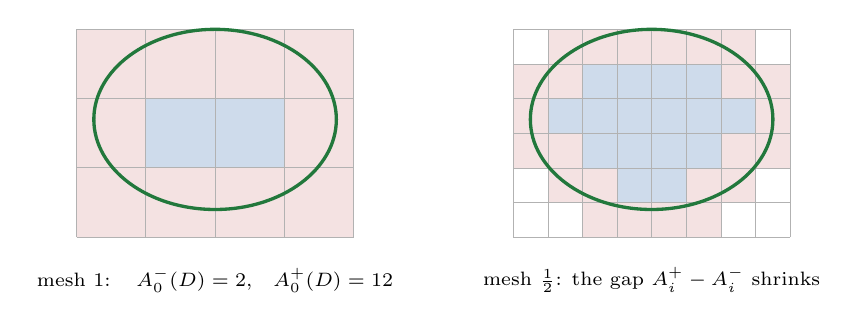
\begin{tikzpicture}[scale=0.88]
% ---- Panel 1: coarse mesh ----
\begin{scope}[shift={(0,0)}]
% outer squares (intersecting D): shade light red; inner squares: shade light blue
% region D: ellipse-ish blob centered (2,1.7), radii 1.75/1.3
% grid of side 1 over [0,4]x[0,3.5]... determine by formula: square [i,i+1]x[j,j+1]
% Precomputed classification for ellipse ((x-2)/1.75)^2+((y-1.7)/1.3)^2 <= 1
% inner: none at mesh 1 except center column squares [1,2]x[1,2],[2,3]x[1,2]? check corners:
% square [1,2]x[1,2]: corners (1,1):((-1)/1.75)^2+((-.7)/1.3)^2=0.327+0.29=0.62<1 ok;(2,1):0+0.29<1;(1,2):0.327+0.053=0.38;(2,2):0.053 -> all inside => inner
% square [2,3]x[1,2]: mirror => inner
% fill outer-only squares light red: those intersecting but not inside
\foreach \i/\j in {0/0,1/0,2/0,3/0,0/1,3/1,0/2,1/2,2/2,3/2}{
  \fill[figR!14] (\i,\j) rectangle ++(1,1);}
\foreach \i/\j in {1/1,2/1}{
  \fill[figB!22] (\i,\j) rectangle ++(1,1);}
% grid
\draw[gray!60, thin] (0,0) grid[step=1] (4,3);
% region boundary
\draw[very thick, figG] (2,1.7) ellipse (1.75 and 1.3);
\node[font=\scriptsize, align=center] at (2,-0.62) {mesh $1$: \; $A_0^-(D) = 2$, \; $A_0^+(D) = 12$};
\end{scope}
% ---- Panel 2: fine mesh (side 1/2) ----
\begin{scope}[shift={(6.3,0)}]
% classify half-squares: side 0.5 over [0,4]x[0,3]
\foreach \i in {0,...,7}{ \foreach \j in {0,...,5}{
  % corners of square [i/2,(i+1)/2] x [j/2,(j+1)/2]
  \pgfmathsetmacro{\xa}{\i/2} \pgfmathsetmacro{\xb}{(\i+1)/2}
  \pgfmathsetmacro{\ya}{\j/2} \pgfmathsetmacro{\yb}{(\j+1)/2}
  \pgfmathsetmacro{\caa}{((\xa-2)/1.75)^2+((\ya-1.7)/1.3)^2}
  \pgfmathsetmacro{\cab}{((\xa-2)/1.75)^2+((\yb-1.7)/1.3)^2}
  \pgfmathsetmacro{\cba}{((\xb-2)/1.75)^2+((\ya-1.7)/1.3)^2}
  \pgfmathsetmacro{\cbb}{((\xb-2)/1.75)^2+((\yb-1.7)/1.3)^2}
  \pgfmathtruncatemacro{\allin}{((\caa<1)&&(\cab<1)&&(\cba<1)&&(\cbb<1)) ? 1 : 0}
  % crude intersect test: any corner inside OR center inside
  \pgfmathsetmacro{\cc}{(((\xa+\xb)/2-2)/1.75)^2+(((\ya+\yb)/2-1.7)/1.3)^2}
  \pgfmathtruncatemacro{\anyin}{((\caa<1)||(\cab<1)||(\cba<1)||(\cbb<1)||(\cc<1)) ? 1 : 0}
  \ifnum\allin>0
    \fill[figB!22] (\xa,\ya) rectangle (\xb,\yb);
  \else
    \ifnum\anyin>0
      \fill[figR!14] (\xa,\ya) rectangle (\xb,\yb);
    \fi
  \fi
}}
\draw[gray!60, ultra thin] (0,0) grid[step=0.5] (4,3);
\draw[very thick, figG] (2,1.7) ellipse (1.75 and 1.3);
\node[font=\scriptsize, align=center] at (2,-0.62) {mesh $\tfrac12$: the gap $A_i^+ - A_i^-$ shrinks};
\end{scope}
\end{tikzpicture}%
\figcap{Inner approximation (blue): squares entirely inside $D$; outer approximation (red $\cup$ blue): squares meeting $D$. Refining the mesh raises $A_i^-$ and lowers $A_i^+$; the region is Jordan measurable when the two limits agree. The mismatch lives entirely along the boundary --- which is why measurability $\iff$ $\partial D$ has content zero.}
\end{center}


\begin{remark}
The difference $A_i^+(D) - A_i^-(D)$ counts squares that straddle the boundary $\partial D$. As $i \to \infty$, these boundary squares have total area $\to 0$ if and only if $\partial D$ has ``measure zero.''

A set $D$ is Jordan measurable $\iff$ its boundary $\partial D$ has Jordan content zero.
\end{remark}

\subsection*{Almost Disjoint Sets}

\begin{definition}[Almost Disjoint]
Two sets $D, E \subseteq \R^2$ are \textbf{almost disjoint} if their interiors do not intersect:
\[
\text{int}(D) \cap \text{int}(E) = \emptyset.
\]
Equivalently, they can only overlap on their boundaries.
\end{definition}

\begin{remark}
Almost disjoint sets can share boundary points, but not interior points. For example, two adjacent squares sharing an edge are almost disjoint.
\end{remark}

\subsection*{Additivity of Jordan Measure}

\begin{theorem}[Additivity]
If $D$ and $E$ are both Jordan measurable and almost disjoint, then $D \cup E$ is Jordan measurable and:
\[
|D \cup E| = |D| + |E|.
\]
\end{theorem}

\begin{proof}
We prove this in two parts: first the upper bound (subadditivity), then the lower bound (superadditivity for almost disjoint sets).

\textbf{Part 1: $A_k^+(D \cup E) \leq A_k^+(D) + A_k^+(E)$ (subadditivity of outer measure).}

Consider $\mathcal{S}_k^+(D \cup E)$, the set of $k$-th level squares intersecting $D \cup E$.

For any square $S$:
\[
S \in \mathcal{S}_k^+(D \cup E) \iff S \cap (D \cup E) \neq \emptyset \iff (S \cap D) \cup (S \cap E) \neq \emptyset \iff S \in \mathcal{S}_k^+(D) \text{ or } S \in \mathcal{S}_k^+(E).
\]

Therefore:
\[
\mathcal{S}_k^+(D \cup E) \subseteq \mathcal{S}_k^+(D) \cup \mathcal{S}_k^+(E).
\]

Counting elements (with possible overlap):
\[
\#\mathcal{S}_k^+(D \cup E) \leq \#\mathcal{S}_k^+(D) + \#\mathcal{S}_k^+(E).
\]

Multiplying by the area of each square $\left(\frac{1}{2^k}\right)^2$:
\[
A_k^+(D \cup E) \leq A_k^+(D) + A_k^+(E).
\]

Taking $k \to \infty$:
\[
\overline{A}(D \cup E) \leq \overline{A}(D) + \overline{A}(E).
\]

\textbf{Part 2: $A_k^-(D) + A_k^-(E) \leq A_k^-(D \cup E)$ (superadditivity of inner measure for almost disjoint sets).}

Since $\text{int}(D) \cap \text{int}(E) = \emptyset$, we claim that $\mathcal{S}_k^-(D) \cap \mathcal{S}_k^-(E) = \emptyset$.

Suppose $S \in \mathcal{S}_k^-(D)$ and $S \in \mathcal{S}_k^-(E)$. Then $S \subseteq D$ and $S \subseteq E$.

Choose the center $\mathbf{x}$ of $S$. Since $S$ is contained in the interior of itself, $\mathbf{x}$ is an interior point of both $D$ and $E$. But this contradicts $\text{int}(D) \cap \text{int}(E) = \emptyset$.

Therefore, $\mathcal{S}_k^-(D)$ and $\mathcal{S}_k^-(E)$ are disjoint.

Also, $\mathcal{S}_k^-(D) \cup \mathcal{S}_k^-(E) \subseteq \mathcal{S}_k^-(D \cup E)$ since:
\[
S \subseteq D \Rightarrow S \subseteq D \cup E, \quad S \subseteq E \Rightarrow S \subseteq D \cup E.
\]

Since $\mathcal{S}_k^-(D)$ and $\mathcal{S}_k^-(E)$ are disjoint:
\[
\#\mathcal{S}_k^-(D) + \#\mathcal{S}_k^-(E) = \#(\mathcal{S}_k^-(D) \cup \mathcal{S}_k^-(E)) \leq \#\mathcal{S}_k^-(D \cup E).
\]

Therefore:
\[
A_k^-(D) + A_k^-(E) \leq A_k^-(D \cup E).
\]

Taking $k \to \infty$:
\[
\underline{A}(D) + \underline{A}(E) \leq \underline{A}(D \cup E).
\]

\textbf{Part 3: Combining the bounds.}

We have:
\[
\underline{A}(D) + \underline{A}(E) \leq \underline{A}(D \cup E) \leq \overline{A}(D \cup E) \leq \overline{A}(D) + \overline{A}(E).
\]

Since $D$ and $E$ are Jordan measurable: $\underline{A}(D) = \overline{A}(D) = |D|$ and $\underline{A}(E) = \overline{A}(E) = |E|$.

Thus:
\[
|D| + |E| \leq \underline{A}(D \cup E) \leq \overline{A}(D \cup E) \leq |D| + |E|.
\]

All inequalities are equalities, so $\underline{A}(D \cup E) = \overline{A}(D \cup E) = |D| + |E|$.

Therefore $D \cup E$ is Jordan measurable with $|D \cup E| = |D| + |E|$.
\end{proof}

\subsection{Definition of the Integral}

Now we define the integral of a function over a Jordan measurable set, analogous to Riemann integration in one dimension.

\begin{definition}[Partition]
Let $D \subseteq \R^2$ be a bounded, Jordan measurable set. A \textbf{partition} of $D$ is a finite collection:
\[
\mathcal{T} = \{D_1, D_2, \ldots, D_N\}
\]
of Jordan measurable sets such that:
\begin{enumerate}
    \item $\bigcup_{i=1}^{N} D_i = D$ \quad (the pieces cover $D$)
    \item $D_i$ and $D_j$ are almost disjoint for $i \neq j$ \quad (interiors don't overlap)
\end{enumerate}
\end{definition}

\begin{definition}[Upper and Lower Sums]
Given a bounded function $f: D \to \R$ and a partition $\mathcal{T} = \{D_1, \ldots, D_N\}$, define:
\[
M_i = \sup_{(x,y) \in D_i} f(x, y), \qquad m_i = \inf_{(x,y) \in D_i} f(x, y).
\]

The \textbf{upper sum} and \textbf{lower sum} are:
\[
U(f, \mathcal{T}) = \sum_{i=1}^{N} M_i |D_i|, \qquad L(f, \mathcal{T}) = \sum_{i=1}^{N} m_i |D_i|.
\]
\end{definition}

\begin{definition}[Diameter and Mesh]
The \textbf{diameter} of a set $A \subseteq \R^2$ is:
\[
\text{diam}(A) = \sup_{\substack{(x, y) \in A \\ (x', y') \in A}} \left| (x, y) - (x', y') \right| = \sup_{\substack{(x, y) \in A \\ (x', y') \in A}} \sqrt{(x - x')^2 + (y - y')^2}.
\]

The \textbf{mesh} (or \textbf{norm}) of a partition $\mathcal{T} = \{D_1, \ldots, D_N\}$ is:
\[
\|\mathcal{T}\| = \max_{1 \leq i \leq N} \text{diam}(D_i).
\]
This measures the ``scale'' of the partition --- the size of the largest piece.
\end{definition}

\begin{definition}[Integrable Function]
A bounded function $f: D \to \R$ is \textbf{integrable} (or \textbf{Riemann integrable}) over $D$ if:
\[
\lim_{\|\mathcal{T}\| \to 0} \sum_{i=1}^{N} (M_i - m_i) |D_i| = 0.
\]

Equivalently, the difference between the upper and lower sums vanishes as the partition becomes finer.
\end{definition}

\begin{center}
\includegraphics[width=0.98\textwidth]{pyfigs/f16_riemann_boxes.pdf}%
\figcap{The two Darboux staircases over the same partition $\mathcal{T}$. Left: the \textnormal{lower sum} $L(f,\mathcal{T}) = \sum m_i |D_i|$ with $m_i = \inf_{D_i} f$ --- inscribed boxes, entirely under the surface. Right: the \textnormal{upper sum} $U(f,\mathcal{T}) = \sum M_i |D_i|$ with $M_i = \sup_{D_i} f$ --- circumscribing boxes, containing the surface. Every Riemann sum with arbitrary sample points is squeezed between them: $L(f,\mathcal{T}) \leq \sum f(\boldsymbol{\xi}_i)|D_i| \leq U(f,\mathcal{T})$. Integrability is exactly the statement that the gap $\sum (M_i - m_i)|D_i|$ --- the skin between the two staircases --- vanishes as $\|\mathcal{T}\| \to 0$; the common limit is $\iint_D f\,dA$. This is the 2D version of the upper/lower Darboux sums from single-variable analysis.}
\end{center}


\begin{remark}
The condition says that as we refine the partition (make $\|\mathcal{T}\| \to 0$), the ``error'' between the upper and lower sums:
\[
U(f, \mathcal{T}) - L(f, \mathcal{T}) = \sum_{i=1}^{N} (M_i - m_i) |D_i|
\]
tends to zero. This is analogous to the Riemann criterion for integrability in one dimension.
\end{remark}

\begin{definition}[The Integral]
If $f$ is integrable over $D$, the \textbf{integral} of $f$ over $D$ is the common limit:
\[
\iint_D f(x, y) \, dA = \lim_{\|\mathcal{T}\| \to 0} U(f, \mathcal{T}) = \lim_{\|\mathcal{T}\| \to 0} L(f, \mathcal{T}).
\]
\end{definition}

\begin{remark}[Notation: $dA$, $dx\,dy$, and $dV$]
The symbol $dA$ denotes the \textbf{area element}. For rectangular partitions in Cartesian coordinates, each piece $D_i$ is a small rectangle with area $|D_i| = \Delta x \cdot \Delta y$. In the limit, we write:
\[
dA = dx \, dy.
\]
Thus, the following notations are equivalent for integrals in Cartesian coordinates:
\[
\iint_D f(x, y) \, dA = \iint_D f(x, y) \, dx \, dy.
\]

In other coordinate systems, $dA$ takes a different form. For example, in polar coordinates:
\[
dA = r \, dr \, d\theta.
\]

For triple integrals in $\R^3$, we use the \textbf{volume element} $dV$:
\[
dV = dx \, dy \, dz \quad \text{(Cartesian)}, \qquad dV = r \, dr \, d\theta \, dz \quad \text{(cylindrical)}, \qquad dV = \rho^2 \sin\phi \, d\rho \, d\phi \, d\theta \quad \text{(spherical)}.
\]

The general principle: when changing coordinates via a transformation with Jacobian $J$, the volume/area element transforms as:
\[
dA_{\text{new}} = |J| \, dA_{\text{old}}.
\]
\end{remark}

\begin{remark}[Evaluating the Integral]
To compute the integral, choose sample points $(\xi_i, \eta_i) \in D_i$ for each piece of the partition. Then:
\[
\iint_D f(x, y) \, dA = \lim_{\|\mathcal{T}\| \to 0} \sum_{i=1}^{N} f(\xi_i, \eta_i) |D_i|.
\]
The limit exists and equals the integral regardless of how the sample points are chosen (as long as $f$ is integrable).
\end{remark}

\subsection{Properties of the Integral}

Throughout, assume $D$ is bounded and Jordan measurable, and all functions are integrable on $D$.

\begin{theorem}[Scalar Multiplication]
If $f$ is integrable on $D$ and $c \in \R$, then $cf$ is integrable on $D$ and:
\[
\iint_D cf \, dA = c \iint_D f \, dA.
\]
\end{theorem}

\begin{proof}
Assume $c > 0$ (the case $c < 0$ is similar, and $c = 0$ is trivial).

For any partition $\mathcal{T}$:
\[
S_{\mathcal{T}}^+(cf) = \sum_{i=1}^{N} \sup_{(x,y) \in D_i} (cf) \cdot |D_i| = \sum_{i=1}^{N} c \cdot \sup_{(x,y) \in D_i} f \cdot |D_i| = c \cdot S_{\mathcal{T}}^+(f).
\]

Similarly, $S_{\mathcal{T}}^-(cf) = c \cdot S_{\mathcal{T}}^-(f)$.

Therefore:
\[
S_{\mathcal{T}}^+(cf) - S_{\mathcal{T}}^-(cf) = c \cdot \left( S_{\mathcal{T}}^+(f) - S_{\mathcal{T}}^-(f) \right).
\]

Since $f$ is integrable, $S_{\mathcal{T}}^+(f) - S_{\mathcal{T}}^-(f) \to 0$ as $\|\mathcal{T}\| \to 0$, so the same holds for $cf$.

To evaluate: choose sample points $(\xi_i, \eta_i) \in D_i$. Then:
\[
\sum_{i=1}^{N} cf(\xi_i, \eta_i) |D_i| = c \sum_{i=1}^{N} f(\xi_i, \eta_i) |D_i| \xrightarrow{\|\mathcal{T}\| \to 0} c \iint_D f \, dA.
\]
\end{proof}

\begin{theorem}[Additivity in the Integrand]
If $f$ and $g$ are integrable on $D$, then $f + g$ is integrable on $D$ and:
\[
\iint_D (f + g) \, dA = \iint_D f \, dA + \iint_D g \, dA.
\]
\end{theorem}

\begin{proof}
\textbf{Step 1: Bound the upper sums.}

For any $(x, y) \in D_i$: $f(x,y) + g(x,y) \leq \sup_{D_i} f + \sup_{D_i} g$.

Taking sup over $(x, y) \in D_i$: $\sup_{D_i}(f + g) \leq \sup_{D_i} f + \sup_{D_i} g$.

Therefore:
\[
S_{\mathcal{T}}^+(f + g) = \sum_{i=1}^{N} \sup_{D_i}(f + g) \cdot |D_i| \leq \sum_{i=1}^{N} \left( \sup_{D_i} f + \sup_{D_i} g \right) |D_i| = S_{\mathcal{T}}^+(f) + S_{\mathcal{T}}^+(g).
\]

\textbf{Step 2: Bound the lower sums.}

Similarly: $\inf_{D_i}(f + g) \geq \inf_{D_i} f + \inf_{D_i} g$.

Therefore:
\[
S_{\mathcal{T}}^-(f + g) \geq S_{\mathcal{T}}^-(f) + S_{\mathcal{T}}^-(g).
\]

\textbf{Step 3: Integrability.}

Combining:
\[
S_{\mathcal{T}}^-(f) + S_{\mathcal{T}}^-(g) \leq S_{\mathcal{T}}^-(f + g) \leq S_{\mathcal{T}}^+(f + g) \leq S_{\mathcal{T}}^+(f) + S_{\mathcal{T}}^+(g).
\]

Since $f$ and $g$ are integrable, both $S_{\mathcal{T}}^+(f) - S_{\mathcal{T}}^-(f) \to 0$ and $S_{\mathcal{T}}^+(g) - S_{\mathcal{T}}^-(g) \to 0$.

By the squeeze theorem, $S_{\mathcal{T}}^+(f+g) - S_{\mathcal{T}}^-(f+g) \to 0$, so $f + g$ is integrable.

\textbf{Step 4: Evaluate the integral.}

Choose sample points $(\xi_i, \eta_i) \in D_i$:
\[
\sum_{i=1}^{N} (f + g)(\xi_i, \eta_i) |D_i| = \sum_{i=1}^{N} f(\xi_i, \eta_i) |D_i| + \sum_{i=1}^{N} g(\xi_i, \eta_i) |D_i|.
\]

As $\|\mathcal{T}\| \to 0$:
\[
\iint_D (f + g) \, dA = \iint_D f \, dA + \iint_D g \, dA.
\]
\end{proof}

\begin{theorem}[Additivity over Domains]
Let $A$ and $B$ be Jordan measurable, almost disjoint sets. If $f$ is integrable on $A$, $B$, and $A \cup B$, then:
\[
\iint_{A \cup B} f \, dA = \iint_A f \, dA + \iint_B f \, dA.
\]
\end{theorem}

\begin{proof}
Let $\mathcal{T}_A$ be a partition of $A$ and $\mathcal{T}_B$ be a partition of $B$.

Then $\mathcal{T}_A \cup \mathcal{T}_B$ is a partition of $A \cup B$ (since $A$ and $B$ are almost disjoint).

If $\|\mathcal{T}_A\| \to 0$ and $\|\mathcal{T}_B\| \to 0$, then $\|\mathcal{T}_A \cup \mathcal{T}_B\| \to 0$.

Suppose $\mathcal{T}_A$ has $N$ pieces and $\mathcal{T}_B$ has $M$ pieces. Then for sample points:
\[
\sum_{i=1}^{N+M} f(\xi_i, \eta_i) |D_i| = \underbrace{\sum_{i=1}^{N} f(\xi_i, \eta_i) |D_i|}_{\text{sum over } \mathcal{T}_A} + \underbrace{\sum_{i=1}^{M} f(\xi_i, \eta_i) |D_i|}_{\text{sum over } \mathcal{T}_B}.
\]

Taking $\|\mathcal{T}_A\|, \|\mathcal{T}_B\| \to 0$:
\[
\iint_{A \cup B} f \, dA = \iint_A f \, dA + \iint_B f \, dA.
\]
\end{proof}

\begin{remark}[On the Intersection and Integrability]
A subtle point in the proof: when we combine $\mathcal{T}_A \cup \mathcal{T}_B$, pieces from $\mathcal{T}_A$ and $\mathcal{T}_B$ may overlap on $A \cap B$ (which lies in the boundaries since $A$ and $B$ are almost disjoint).

Why doesn't this cause problems?
\begin{itemize}
    \item Since $A$ and $B$ are almost disjoint, $A \cap B \subseteq \partial A \cap \partial B$.
    \item For Jordan measurable sets, the boundary has Jordan content zero: $|A \cap B| = 0$.
    \item Any contribution from the intersection region has measure zero and doesn't affect the integral.
\end{itemize}

More precisely, if a piece $D_i \in \mathcal{T}_A$ overlaps with a piece $D_j \in \mathcal{T}_B$, their overlap $D_i \cap D_j$ has Jordan content zero (it's contained in $A \cap B$). So even if we ``double-count'' this region, it contributes zero to both sums.

This is why we need the hypothesis that $A$ and $B$ are \textbf{Jordan measurable} (not just arbitrary sets) --- the boundary must have content zero for the additivity to work cleanly.
\end{remark}

\begin{remark}
To evaluate the integral, we only need \emph{one} sequence of partitions whose mesh goes to zero. The limit is the same regardless of how we partition or where we choose sample points.
\end{remark}

\subsection*{Comparison / Mean-Value Property}

\begin{theorem}[Comparison Theorem]
If $f$ and $g$ are integrable on $D$ and $f \leq g$ on $D$, then:
\[
\iint_D f \, dA \leq \iint_D g \, dA.
\]
\end{theorem}

\begin{proof}
It suffices to show: if $f \geq 0$ on $D$, then $\iint_D f \, dA \geq 0$.

This follows directly from the definition: for any partition $\mathcal{T}$ and sample points $(\xi_i, \eta_i) \in D_i$:
\[
\sum_{i=1}^{N} f(\xi_i, \eta_i) |D_i| \geq 0
\]
since each $f(\xi_i, \eta_i) \geq 0$ and $|D_i| \geq 0$.

Taking the limit as $\|\mathcal{T}\| \to 0$ preserves the inequality.

For the general case: if $f \leq g$, then $g - f \geq 0$, so $\iint_D (g - f) \, dA \geq 0$, which gives $\iint_D g \, dA \geq \iint_D f \, dA$.
\end{proof}

\begin{corollary}[Absolute Value Inequality]
If $f$ is integrable on $D$, then $|f|$ is integrable and:
\[
\left| \iint_D f \, dA \right| \leq \iint_D |f| \, dA.
\]
\end{corollary}

\begin{proof}
Since $-|f| \leq f \leq |f|$, by the comparison theorem:
\[
-\iint_D |f| \, dA \leq \iint_D f \, dA \leq \iint_D |f| \, dA.
\]
\end{proof}

\subsection*{Iterated Integrals: The Simple Case}

Consider the simple case where $D = [a, b] \times [c, d]$ is a rectangle.

Suppose $f$ is integrable on $D$. Partition:
\begin{itemize}
    \item $[a, b]$ into $N$ pieces of width $h = \frac{b-a}{N}$
    \item $[c, d]$ into $M$ pieces of width $k = \frac{d-c}{M}$
\end{itemize}

This gives $N \times M$ small rectangles $D_{ij} = [a + (i-1)h, a + ih] \times [c + (j-1)k, c + jk]$.

The Riemann sum is:
\[
\sum_{i=1}^{N} \sum_{j=1}^{M} f(a + (i-1)h + \theta h, c + (j-1)k + \lambda k) \cdot hk
\]
for some $\theta, \lambda \in [0, 1]$ (or we can choose any sample point in $D_{ij}$).

Taking $h, k \to 0$ (i.e., $N, M \to \infty$):
\[
\iint_D f(x, y) \, dA = \int_a^b \int_c^d f(x, y) \, dy \, dx = \int_c^d \int_a^b f(x, y) \, dx \, dy.
\]

\subsection*{Change of Variables: Polar Coordinates}

\begin{theorem}[Change of Variables to Polar Coordinates]
Let $D^* = \{(r, \theta) : a \leq r \leq b, \alpha \leq \theta \leq \beta\}$ be a region in polar coordinates, and let $D \subseteq \R^2$ be its image under the transformation $x = r\cos\theta$, $y = r\sin\theta$.

If $f$ is continuous on $D$, then:
\[
\iint_D f(x, y) \, dx\, dy = \int_\alpha^\beta \int_a^b f(r\cos\theta, r\sin\theta) \cdot r \, dr \, d\theta.
\]

The factor $r$ is the absolute value of the Jacobian: $\left| \dfrac{\partial(x, y)}{\partial(r, \theta)} \right| = r$.
\end{theorem}

\begin{proof}
We prove this directly from the definition of the integral by computing areas of polar rectangles.

\textbf{Step 1: Partition the polar region.}

Partition:
\begin{itemize}
    \item $[a, b]$ into $M$ pieces of width $k = \frac{b-a}{M}$: radii $r_i = a + ik$ for $i = 0, 1, \ldots, M$.
    \item $[\alpha, \beta]$ into $N$ pieces of width $h = \frac{\beta - \alpha}{N}$: angles $\theta_j = \alpha + jh$ for $j = 0, 1, \ldots, N$.
\end{itemize}

This gives $M \times N$ polar rectangles $D_{ij}^*$ with:
\begin{itemize}
    \item Inner radius: $r_{i-1} = a + (i-1)k$
    \item Outer radius: $r_i = a + ik$
    \item Angular span: from $\theta_{j-1} = \alpha + (j-1)h$ to $\theta_j = \alpha + jh$
\end{itemize}

\textbf{Step 2: Compute the area of each polar rectangle.}

The area of a circular sector with radii $r_1$ to $r_2$ and angle $\Delta\theta$ is:
\[
\text{Area} = \frac{\Delta\theta}{2\pi} \cdot \pi r_2^2 - \frac{\Delta\theta}{2\pi} \cdot \pi r_1^2 = \frac{\Delta\theta}{2}(r_2^2 - r_1^2).
\]

For the $(i, j)$-th polar rectangle with $r_1 = a + (i-1)k$, $r_2 = a + ik$, $\Delta\theta = h$:
\[
|D_{ij}| = \frac{h}{2}\left( (a + ik)^2 - (a + (i-1)k)^2 \right).
\]

\textbf{Step 3: Expand the area formula.}

\begin{align*}
(a + ik)^2 - (a + (i-1)k)^2 &= \left[ a^2 + 2aik + i^2k^2 \right] - \left[ a^2 + 2a(i-1)k + (i-1)^2k^2 \right] \\
&= 2ak + \left( i^2 - (i-1)^2 \right) k^2 \\
&= 2ak + (2i - 1)k^2.
\end{align*}

Therefore:
\[
|D_{ij}| = \frac{h}{2}\left( 2ak + (2i-1)k^2 \right) = hk \left( a + \frac{(2i-1)k}{2} \right) = hk \cdot \bar{r}_i
\]
where $\bar{r}_i = a + (i - \frac{1}{2})k$ is the midpoint radius of the $i$-th annular strip.

\textbf{Step 4: Form the Riemann sum.}

Choose sample points in polar coordinates: $(\bar{r}_i, \bar{\theta}_j)$ where $\bar{r}_i = a + (i - \frac{1}{2})k$ and $\bar{\theta}_j = \alpha + (j - \frac{1}{2})h$.

In Cartesian coordinates, these are:
\[
(x_{ij}, y_{ij}) = (\bar{r}_i \cos\bar{\theta}_j, \bar{r}_i \sin\bar{\theta}_j).
\]

The Riemann sum for $\iint_D f(x, y) \, dA$ is:
\[
\sum_{i=1}^{M} \sum_{j=1}^{N} f(x_{ij}, y_{ij}) \cdot |D_{ij}| = \sum_{i=1}^{M} \sum_{j=1}^{N} f(\bar{r}_i \cos\bar{\theta}_j, \bar{r}_i \sin\bar{\theta}_j) \cdot \bar{r}_i \cdot hk.
\]

\textbf{Step 5: Recognize as a Riemann sum in $(r, \theta)$.}

Define $g(r, \theta) = f(r\cos\theta, r\sin\theta) \cdot r$. Then:
\[
\sum_{i=1}^{M} \sum_{j=1}^{N} f(\bar{r}_i \cos\bar{\theta}_j, \bar{r}_i \sin\bar{\theta}_j) \cdot \bar{r}_i \cdot hk = \sum_{i=1}^{M} \sum_{j=1}^{N} g(\bar{r}_i, \bar{\theta}_j) \cdot hk.
\]

This is exactly a Riemann sum for $\iint_{D^*} g(r, \theta) \, dr\, d\theta$ over the rectangle $[a, b] \times [\alpha, \beta]$.

\textbf{Step 6: Take the limit.}

As $M, N \to \infty$ (i.e., $h, k \to 0$):
\[
\iint_D f(x, y) \, dx\, dy = \lim_{M, N \to \infty} \sum_{i=1}^{M} \sum_{j=1}^{N} g(\bar{r}_i, \bar{\theta}_j) \cdot hk = \iint_{D^*} g(r, \theta) \, dr\, d\theta.
\]

By Fubini's theorem on the rectangle $[a, b] \times [\alpha, \beta]$:
\[
\iint_D f(x, y) \, dx\, dy = \int_\alpha^\beta \int_a^b f(r\cos\theta, r\sin\theta) \cdot r \, dr \, d\theta.
\]
\end{proof}

\begin{remark}[The Jacobian]
The factor $r$ appearing in the integrand is the \textbf{Jacobian} of the polar coordinate transformation:
\[
x = r\cos\theta, \quad y = r\sin\theta.
\]
\[
J = \frac{\partial(x, y)}{\partial(r, \theta)} = \det \begin{pmatrix} \dfrac{\partial x}{\partial r} & \dfrac{\partial x}{\partial \theta} \\[8pt] \dfrac{\partial y}{\partial r} & \dfrac{\partial y}{\partial \theta} \end{pmatrix} = \det \begin{pmatrix} \cos\theta & -r\sin\theta \\ \sin\theta & r\cos\theta \end{pmatrix} = r\cos^2\theta + r\sin^2\theta = r.
\]

The proof above shows \emph{why} the Jacobian appears: it measures how the transformation distorts area. A small rectangle $dr \times d\theta$ in polar coordinates maps to a region of area approximately $r \cdot dr \cdot d\theta$ in Cartesian coordinates.
\end{remark}

\begin{center}
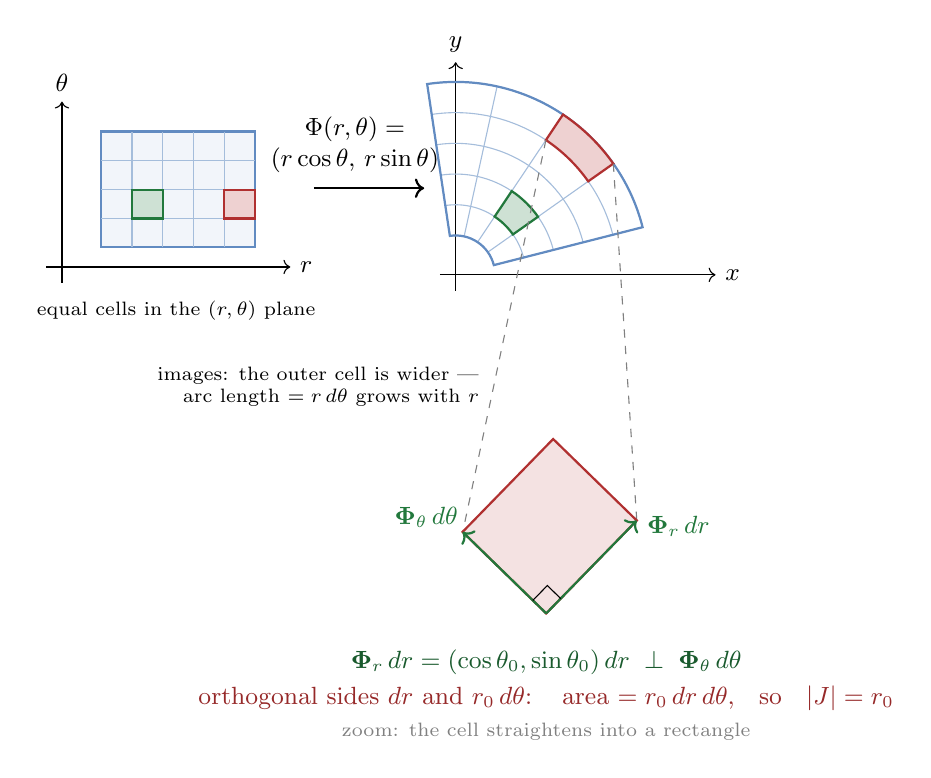
\begin{tikzpicture}[scale=1.0]
% ======== TOP LEFT: (r,theta) rectangle grid ========
\begin{scope}
\draw[->] (-0.2,0) -- (2.9,0) node[right, font=\small] {$r$};
\draw[->] (0,-0.2) -- (0,2.1) node[above, font=\small] {$\theta$};
\draw[thick, figB!70, fill=figB!6] (0.5,0.25) rectangle (2.45,1.72);
% grid: r lines at 0.5,0.89,1.28,1.67,2.06,2.45 ; theta at 0.25,0.615,0.98,1.355,1.72
\foreach \r in {0.89,1.28,1.67,2.06} \draw[figB!40, thin] (\r,0.25) -- (\r,1.72);
\foreach \t in {0.615,0.98,1.355} \draw[figB!40, thin] (0.5,\t) -- (2.45,\t);
% two same-size cells: inner-r and outer-r
\draw[thick, figG, fill=figG!22] (0.89,0.615) rectangle (1.28,0.98);
\draw[thick, figR, fill=figR!22] (2.06,0.615) rectangle (2.45,0.98);
\node[font=\scriptsize, align=center] at (1.45,-0.55) {equal cells in the $(r,\theta)$ plane};
\end{scope}
% map arrow
\draw[->, thick] (3.2,1.0) -- (4.6,1.0);
\node[font=\small, align=center] at (3.72,1.55) {$\Phi(r,\theta)=$\\ $(r\cos\theta,\, r\sin\theta)$};
% ======== TOP RIGHT: polar image ========
\begin{scope}[shift={(5.0,-0.1)}]
\draw[->] (-0.2,0) -- (3.3,0) node[right, font=\small] {$x$};
\draw[->] (0,-0.2) -- (0,2.7) node[above, font=\small] {$y$};
% sector between theta=0.25 and 1.72 rad, r from 0.5 to 2.45
% arcs at r values
\foreach \r in {0.5,0.89,1.28,1.67,2.06,2.45}
  \draw[figB!40, thin] ({\r*cos(14.3)},{\r*sin(14.3)}) arc[start angle=14.3, end angle=98.5, radius=\r];
% rays at theta values (deg): 14.3, 35.2, 56.2, 77.6, 98.5
\foreach \t in {14.3,35.2,56.2,77.6,98.5}
  \draw[figB!40, thin] ({0.5*cos(\t)},{0.5*sin(\t)}) -- ({2.45*cos(\t)},{2.45*sin(\t)});
% boundary of the sector (thick)
\draw[thick, figB!70]
  ({0.5*cos(14.3)},{0.5*sin(14.3)}) arc[start angle=14.3, end angle=98.5, radius=0.5]
  -- ({2.45*cos(98.5)},{2.45*sin(98.5)})
  arc[start angle=98.5, end angle=14.3, radius=2.45] -- cycle;
% image cells: inner (green) r in [0.89,1.28], theta in [35.2,56.2]; outer (red) r in [2.06,2.45]
\draw[thick, figG, fill=figG!22]
  ({0.89*cos(35.2)},{0.89*sin(35.2)}) arc[start angle=35.2, end angle=56.2, radius=0.89]
  -- ({1.28*cos(56.2)},{1.28*sin(56.2)})
  arc[start angle=56.2, end angle=35.2, radius=1.28] -- cycle;
\draw[thick, figR, fill=figR!22]
  ({2.06*cos(35.2)},{2.06*sin(35.2)}) arc[start angle=35.2, end angle=56.2, radius=2.06]
  -- ({2.45*cos(56.2)},{2.45*sin(56.2)})
  arc[start angle=56.2, end angle=35.2, radius=2.45] -- cycle;
\node[font=\scriptsize, align=right, anchor=east] at (0.42,-1.42) {images: the outer cell is wider ---\\ arc length $= r\,d\theta$ grows with $r$};
\end{scope}
% ======== BOTTOM: zoom of the outer cell ========
\draw[dashed, gray] (6.146,1.612) -- (5.09,-3.365);
\draw[dashed, gray] (7.002,1.312) -- (7.30,-3.22);
\begin{scope}[shift={(5.55,-4.4)}]
% magnified cell: nearly a rectangle, radial side dr, tangential side r0 dtheta
% at theta0=45.7deg: radial dir (0.698,0.716); tangential (-0.716,0.698)
\coordinate (O) at (0.6,0);
\coordinate (Ar) at (1.15,1.18);    % Phi_r dr direction scaled
\coordinate (At) at (-1.18,1.15);   % Phi_theta dtheta (longer: r0 dtheta)
\draw[thick, figR, fill=figR!14] (O) -- ($(O)+(Ar)$) -- ($(O)+(Ar)+0.9*(At)$) -- ($(O)+0.9*(At)$) -- cycle;
\draw[->, thick, figG] (O) -- ($(O)+(Ar)$) node[right, font=\small, yshift=-2pt] {$\boldsymbol{\Phi}_r\,dr$};
\draw[->, thick, figG] (O) -- ($(O)+0.9*(At)$) node[above left=-2pt, font=\small] {$\boldsymbol{\Phi}_\theta\,d\theta$};
% right angle mark
\draw[thin] ($(O)+0.16*(Ar)$) -- ($(O)+0.16*(Ar)+0.144*(At)$) -- ($(O)+0.144*(At)$);
\node[font=\small, figG!75!black] at (0.6,-0.62) {$\boldsymbol{\Phi}_r\,dr = (\cos\theta_0,\sin\theta_0)\,dr \;\perp\; \boldsymbol{\Phi}_\theta\,d\theta$};
\node[font=\small, figR!85!black] at (0.6,-1.08) {orthogonal sides $dr$ and $r_0\,d\theta$: \; area $= r_0\,dr\,d\theta$, \; so \; $|J| = r_0$};
\node[font=\scriptsize, gray] at (0.6,-1.50) {zoom: the cell straightens into a rectangle};
\end{scope}
\end{tikzpicture}%
\figcap{The Jacobian of the polar map $\Phi(r,\theta) = (r\cos\theta, r\sin\theta)$, seen three ways. Top: equal cells in the $(r,\theta)$ plane map to annular cells whose width grows with $r$ --- the distortion is position-dependent. Bottom: zooming into one cell, the map straightens into its derivative $D\Phi$, sending the square to a rectangle with orthogonal sides $|\boldsymbol{\Phi}_r|\,dr = dr$ and $|\boldsymbol{\Phi}_\theta|\,d\theta = r_0\,d\theta$; hence $dx\,dy = r\,dr\,d\theta$ --- the factor in every polar integral of \S15 is literally the width of the cell. At $r = 0$ the tangential side collapses, $J = 0$, and $\Phi$ degenerates (all $\theta$ give the same point): the Inverse Function Theorem's hypothesis fails exactly where polar coordinates fail.}
\end{center}


\subsection{Fubini's Theorem: Rigorous Treatment}

Fubini's theorem allows us to compute double integrals as iterated single integrals and to change the order of integration. We develop this carefully.

\begin{theorem}[Fubini's Theorem --- Rectangle Case]
Let $f: [a, b] \times [c, d] \to \R$ be continuous. Then:
\[
\iint_{[a,b] \times [c,d]} f(x, y) \, dA = \int_a^b \left( \int_c^d f(x, y) \, dy \right) dx = \int_c^d \left( \int_a^b f(x, y) \, dx \right) dy.
\]
\end{theorem}

\begin{center}
\includegraphics[width=0.72\textwidth]{pyfigs/f21_fubini.pdf}%
\figcap{Fubini's theorem geometrically: freeze $x$ and integrate over $y$ to get the cross-sectional area $A(x)$ (red slab); then integrate $A(x)$ over $x$ to stack the slabs into the volume. The iterated integral $\int\!\!\int f\,dy\,dx$ is this two-stage process; Fubini says it equals the double integral whenever $f$ is integrable.}
\end{center}


\begin{proof}
We prove the first equality; the second follows by symmetry.

\textbf{Step 1: Setup the partitions.}

Partition $[a, b]$ into $N$ equal subintervals of width $h = \frac{b-a}{N}$:
\[
a = x_0 < x_1 < \cdots < x_N = b, \quad x_i = a + ih.
\]

Partition $[c, d]$ into $M$ equal subintervals of width $k = \frac{d-c}{M}$:
\[
c = y_0 < y_1 < \cdots < y_M = d, \quad y_j = c + jk.
\]

This gives $N \times M$ small rectangles $R_{ij} = [x_{i-1}, x_i] \times [y_{j-1}, y_j]$, each with area $hk$.

\textbf{Step 2: Riemann sum for the double integral.}

Choose sample points $(\xi_i, \eta_j) \in R_{ij}$. The Riemann sum is:
\[
S_{N,M} = \sum_{i=1}^{N} \sum_{j=1}^{M} f(\xi_i, \eta_j) \cdot hk.
\]

As $N, M \to \infty$ (equivalently, $h, k \to 0$):
\[
S_{N,M} \to \iint_{[a,b] \times [c,d]} f(x, y) \, dA.
\]

\textbf{Step 3: Riemann sum for the iterated integral.}

For the iterated integral, first fix $x = \xi_i$ and consider the inner integral:
\[
F(x) = \int_c^d f(x, y) \, dy.
\]

The Riemann sum for $F(\xi_i)$ is:
\[
\sum_{j=1}^{M} f(\xi_i, \eta_j) \cdot k \approx F(\xi_i) = \int_c^d f(\xi_i, y) \, dy.
\]

Then the Riemann sum for the outer integral $\int_a^b F(x) \, dx$ is:
\[
\sum_{i=1}^{N} F(\xi_i) \cdot h \approx \int_a^b F(x) \, dx = \int_a^b \left( \int_c^d f(x, y) \, dy \right) dx.
\]

\textbf{Step 4: Connect the two.}

Observe that:
\[
\sum_{i=1}^{N} \left( \sum_{j=1}^{M} f(\xi_i, \eta_j) \cdot k \right) h = \sum_{i=1}^{N} \sum_{j=1}^{M} f(\xi_i, \eta_j) \cdot hk = S_{N,M}.
\]

So the Riemann sum for the double integral equals the iterated Riemann sum.

\textbf{Step 5: Take the limit.}

Since $f$ is continuous on the compact set $[a,b] \times [c,d]$, it is uniformly continuous. This ensures:
\begin{itemize}
    \item The inner integral $F(x) = \int_c^d f(x, y) \, dy$ exists for each $x$ and is continuous in $x$.
    \item The Riemann sums converge uniformly.
\end{itemize}

Taking $N, M \to \infty$:
\[
\iint_{[a,b] \times [c,d]} f(x, y) \, dA = \lim_{N,M \to \infty} S_{N,M} = \int_a^b \left( \int_c^d f(x, y) \, dy \right) dx.
\]
\end{proof}

\begin{remark}[Why Continuity Matters]
The key point is that $F(x) = \int_c^d f(x, y) \, dy$ must be well-defined and integrable. Continuity of $f$ guarantees this. 

More generally, Fubini's theorem holds if $f$ is \textbf{integrable} and the iterated integrals exist. The condition can be weakened to: $\iint_D |f| \, dA < \infty$ (absolute integrability).
\end{remark}

\subsection*{Fubini's Theorem for General Regions}

\begin{definition}[Type I and Type II Regions]
A \textbf{Type I region} (vertically simple) is:
\[
D = \{(x, y) : a \leq x \leq b, \; g_1(x) \leq y \leq g_2(x)\}
\]
where $g_1, g_2: [a, b] \to \R$ are continuous with $g_1(x) \leq g_2(x)$.

A \textbf{Type II region} (horizontally simple) is:
\[
D = \{(x, y) : c \leq y \leq d, \; h_1(y) \leq x \leq h_2(y)\}
\]
where $h_1, h_2: [c, d] \to \R$ are continuous with $h_1(y) \leq h_2(y)$.
\end{definition}

\begin{theorem}[Fubini for Type I Regions]
If $D = \{(x, y) : a \leq x \leq b, \; g_1(x) \leq y \leq g_2(x)\}$ and $f$ is continuous on $D$, then:
\[
\iint_D f(x, y) \, dA = \int_a^b \left( \int_{g_1(x)}^{g_2(x)} f(x, y) \, dy \right) dx.
\]
\end{theorem}

\begin{proof}
We give a detailed proof that carefully controls the error from approximating the curved region with rectangles.

\textbf{Setup and assumptions.}

Let $D = \{(x, y) : a \leq x \leq b, \; \psi(x) \leq y \leq \varphi(x)\}$ where $\psi, \varphi: [a,b] \to \R$ are continuous with $\psi(x) \leq \varphi(x)$ for all $x \in [a, b]$.

\textit{Claim: $D$ is closed.} 

Suppose $(x_k, y_k) \in D$ and $(x_k, y_k) \to (x_0, y_0)$. Then $x_k \to x_0$ and $y_k \to y_0$. Since $(x_k, y_k) \in D$:
\[
a \leq x_k \leq b \quad \text{and} \quad \psi(x_k) \leq y_k \leq \varphi(x_k).
\]
Taking $k \to \infty$: since $[a,b]$ is closed, $a \leq x_0 \leq b$. By continuity of $\psi$ and $\varphi$:
\[
\psi(x_0) = \lim_{k \to \infty} \psi(x_k) \leq \lim_{k \to \infty} y_k = y_0 \leq \lim_{k \to \infty} \varphi(x_k) = \varphi(x_0).
\]
Thus $(x_0, y_0) \in D$, so $D$ is closed.

\textit{Boundedness.} Since $D$ is closed and bounded (contained in $[a, b] \times [\min \psi, \max \varphi]$), $D$ is compact. Since $f$ is continuous on the compact set $D$, $f$ is bounded: there exists $B > 0$ such that $|f(x, y)| \leq B$ for all $(x, y) \in D$.

Without loss of generality, embed $D$ in a square $[0, M] \times [0, M]$ for some $M > 0$.

\textbf{Step 1: Partition the square into a grid.}

Fix $\varepsilon > 0$. We will show the difference between the double integral and the iterated integral is $< C\varepsilon$ for some constant $C$ depending only on $B$ and $M$.

Choose $k \in \N$ large (to be determined). Partition $[0, M]$ into $M \cdot 2^k$ intervals of width $h = \frac{1}{2^k}$:
\[
0 = t_0 < t_1 < t_2 < \cdots < t_{M \cdot 2^k} = M, \quad t_i = \frac{i}{2^k}.
\]

This creates a grid of $(M \cdot 2^k)^2$ small squares, each of side $h = \frac{1}{2^k}$ and area $h^2 = \frac{1}{4^k}$.

\textbf{Step 2: Use uniform continuity to control oscillation of boundary curves.}

Since $\psi$ and $\varphi$ are continuous on the compact interval $[a, b]$, they are \textbf{uniformly continuous}.

Thus, for our fixed $\varepsilon > 0$, there exists $\delta > 0$ such that:
\[
|x - x'| < \delta \implies |\varphi(x) - \varphi(x')| < \varepsilon \quad \text{and} \quad |\psi(x) - \psi(x')| < \varepsilon.
\]

Choose $k$ large enough that $\frac{1}{2^k} < \delta$. Then within any column of width $\frac{1}{2^k}$:
\[
\sup_{x \in [t_i, t_{i+1}]} \varphi(x) - \inf_{x \in [t_i, t_{i+1}]} \varphi(x) < \varepsilon.
\]

Similarly for $\psi$. This means: \textit{within each column, the curves $\varphi$ and $\psi$ oscillate by less than $\varepsilon$}.

\textbf{Step 3: Define approximating step functions.}

For each column $[t_i, t_{i+1}]$ intersecting $[a, b]$, define:
\begin{align*}
\varphi_k(x) &= \text{smallest grid value } \geq \sup_{x' \in [t_i, t_{i+1}]} \varphi(x') \quad \text{for } x \in [t_i, t_{i+1}] \\
\psi_k(x) &= \text{largest grid value } \leq \inf_{x' \in [t_i, t_{i+1}]} \psi(x') \quad \text{for } x \in [t_i, t_{i+1}]
\end{align*}

In other words:
\begin{itemize}
    \item $\varphi_k$ rounds $\varphi$ up to the nearest grid line (within each column, taking the sup first).
    \item $\psi_k$ rounds $\psi$ down to the nearest grid line (within each column, taking the inf first).
\end{itemize}

Then $\varphi_k$ and $\psi_k$ are step functions constant on each column, and:
\[
\psi_k(x) \leq \psi(x) \leq \varphi(x) \leq \varphi_k(x) \quad \text{for all } x \in [a, b].
\]

Also, define $a_k$ = largest grid point $\leq a$, and $b_k$ = smallest grid point $\geq b$.

\textbf{Step 4: Define the rectangular approximation $D_k$.}

Let:
\[
D_k = \{(x, y) : a_k \leq x \leq b_k, \; \psi_k(x) \leq y \leq \varphi_k(x)\}.
\]

This is a union of grid squares that contains $D$: specifically, $D \subseteq D_k$.

The region $D_k$ is a ``staircase'' approximation to $D$, where each column consists of a stack of complete grid squares.

\textbf{Step 5: Estimate the area of $D_k \setminus D$ (the error region).}

The error region $D_k \setminus D$ consists of:
\begin{enumerate}
    \item \textbf{Top boundary squares:} In each column $[t_i, t_{i+1}]$, the squares between $y = \varphi(x)$ and $y = \varphi_k(x)$.
    
    Since $\sup \varphi - \inf \varphi < \varepsilon$ within the column (by uniform continuity), and $\varphi_k$ is the next grid line above $\sup \varphi$:
    \[
    \varphi_k(x) - \varphi(x) < \varepsilon + \frac{1}{2^k} < 2\varepsilon
    \]
    for $k$ large enough that $\frac{1}{2^k} < \varepsilon$.
    
    \item \textbf{Bottom boundary squares:} Similarly, $\psi(x) - \psi_k(x) < 2\varepsilon$.
    
    \item \textbf{Left boundary:} The strip from $x = a_k$ to $x = a$ has width $\leq \frac{1}{2^k} < \varepsilon$ and height $\leq M$.
    
    \item \textbf{Right boundary:} The strip from $x = b$ to $x = b_k$ has width $\leq \frac{1}{2^k} < \varepsilon$ and height $\leq M$.
\end{enumerate}

Number of columns intersecting $[a, b]$: at most $(b - a) \cdot 2^k + 2 \leq M \cdot 2^k + 2$.

Area contributed by top boundary squares in each column: $\leq 2\varepsilon \cdot \frac{1}{2^k}$.

Total area from top boundary: $\leq 2\varepsilon \cdot \frac{1}{2^k} \cdot (M \cdot 2^k + 2) = 2\varepsilon(M + \frac{2}{2^k}) < 2\varepsilon(M + 1)$.

Similarly for bottom boundary.

Left/right boundary areas: each $\leq \varepsilon \cdot M$.

Total:
\[
|D_k \setminus D| \leq 2\varepsilon(M+1) + 2\varepsilon(M+1) + 2\varepsilon M = \varepsilon(6M + 4).
\]

\textbf{Step 6: Compare integrals over $D$ and $D_k$.}

Since $D \subseteq D_k$:
\[
\left| \iint_D f \, dA - \iint_{D_k} f \, dA \right| = \left| \iint_{D_k \setminus D} f \, dA \right| \leq \iint_{D_k \setminus D} |f| \, dA \leq B \cdot |D_k \setminus D| \leq B\varepsilon(6M + 4).
\]

\textbf{Step 7: Apply Fubini for rectangles to $D_k$.}

The key observation: $D_k$ is a union of grid squares, and within each column $[t_i, t_{i+1}]$, the region is a rectangle $[t_i, t_{i+1}] \times [\psi_k(x), \varphi_k(x)]$ (where $\psi_k, \varphi_k$ are constant on this column).

By Fubini's theorem for rectangles (applied column by column):
\[
\iint_{D_k} f \, dA = \int_{a_k}^{b_k} \left( \int_{\psi_k(x)}^{\varphi_k(x)} f(x, y) \, dy \right) dx.
\]

\textbf{Step 8: Compare the iterated integrals.}

We need to compare:
\[
\int_{a_k}^{b_k} \int_{\psi_k(x)}^{\varphi_k(x)} f \, dy \, dx \quad \text{vs.} \quad \int_a^b \int_{\psi(x)}^{\varphi(x)} f \, dy \, dx.
\]

For each fixed $x \in [a, b]$, since $\psi_k(x) \leq \psi(x) \leq \varphi(x) \leq \varphi_k(x)$:
\begin{align*}
\left| \int_{\psi_k(x)}^{\varphi_k(x)} f \, dy - \int_{\psi(x)}^{\varphi(x)} f \, dy \right| &= \left| \int_{\psi_k(x)}^{\psi(x)} f \, dy + \int_{\varphi(x)}^{\varphi_k(x)} f \, dy \right| \\
&\leq \int_{\psi_k(x)}^{\psi(x)} |f| \, dy + \int_{\varphi(x)}^{\varphi_k(x)} |f| \, dy \\
&\leq B(\psi(x) - \psi_k(x)) + B(\varphi_k(x) - \varphi(x)) \\
&\leq B \cdot 2\varepsilon + B \cdot 2\varepsilon = 4B\varepsilon.
\end{align*}

Integrating over $x$:
\[
\left| \int_a^b \int_{\psi_k(x)}^{\varphi_k(x)} f \, dy \, dx - \int_a^b \int_{\psi(x)}^{\varphi(x)} f \, dy \, dx \right| \leq \int_a^b 4B\varepsilon \, dx = 4B\varepsilon(b - a) \leq 4BM\varepsilon.
\]

Also, the integrals over $[a_k, a]$ and $[b, b_k]$ contribute:
\[
\left| \int_{a_k}^{a} \int_{\psi_k}^{\varphi_k} f \, dy \, dx \right| \leq B \cdot M \cdot (a - a_k) \leq BM\varepsilon.
\]
Similarly for $[b, b_k]$. Total contribution from left/right strips: $\leq 2BM\varepsilon$.

\textbf{Step 9: Combine all estimates.}

\begin{align*}
&\left| \iint_D f \, dA - \int_a^b \int_{\psi(x)}^{\varphi(x)} f \, dy \, dx \right| \\
&\leq \left| \iint_D f \, dA - \iint_{D_k} f \, dA \right| + \left| \iint_{D_k} f \, dA - \int_{a_k}^{b_k} \int_{\psi_k}^{\varphi_k} f \, dy \, dx \right| \\
&\quad + \left| \int_{a_k}^{b_k} \int_{\psi_k}^{\varphi_k} f \, dy \, dx - \int_a^b \int_{\psi}^{\varphi} f \, dy \, dx \right| \\
&\leq B\varepsilon(6M + 4) + 0 + (4BM\varepsilon + 2BM\varepsilon) \\
&= B\varepsilon(6M + 4 + 6M) = B\varepsilon(12M + 4).
\end{align*}

The middle term is $0$ because Fubini for rectangles gives exact equality for $D_k$.

\textbf{Step 10: Conclusion.}

Let $C = B(12M + 4)$. We have shown:
\[
\left| \iint_D f \, dA - \int_a^b \int_{\psi(x)}^{\varphi(x)} f \, dy \, dx \right| \leq C\varepsilon.
\]

Since $\varepsilon > 0$ was arbitrary and $C$ is independent of $\varepsilon$, the left side must equal $0$:
\[
\iint_D f(x, y) \, dA = \int_a^b \left( \int_{\psi(x)}^{\varphi(x)} f(x, y) \, dy \right) dx. \qedhere
\]
\end{proof}

\begin{theorem}[Fubini for Type II Regions]
If $D = \{(x, y) : c \leq y \leq d, \; h_1(y) \leq x \leq h_2(y)\}$ and $f$ is continuous on $D$, then:
\[
\iint_D f(x, y) \, dA = \int_c^d \left( \int_{h_1(y)}^{h_2(y)} f(x, y) \, dx \right) dy.
\]
\end{theorem}

\begin{proof}
The proof is identical to the Type I case, with the roles of $x$ and $y$ interchanged. The region is approximated by horizontal stacks of rectangles, and uniform continuity of $h_1, h_2$ controls the boundary oscillation.
\end{proof}

\subsection*{Changing the Order of Integration}

\begin{corollary}[Changing Order of Integration]
If $D$ is both Type I and Type II (i.e., can be described either way), and $f$ is continuous on $D$, then:
\[
\int_a^b \int_{g_1(x)}^{g_2(x)} f(x, y) \, dy \, dx = \int_c^d \int_{h_1(y)}^{h_2(y)} f(x, y) \, dx \, dy.
\]
\end{corollary}

\begin{proof}
Both iterated integrals equal $\iint_D f \, dA$ by the Type I and Type II versions of Fubini's theorem.
\end{proof}

\begin{remark}[When to Change Order]
Changing the order of integration is useful when:
\begin{itemize}
    \item One order leads to an integral that is difficult or impossible to evaluate in closed form.
    \item The other order simplifies the computation.
\end{itemize}
The key step is to carefully describe the region $D$ in both Type I and Type II forms.
\end{remark}

\begin{example}[Changing Order of Integration]
Evaluate $\displaystyle \int_0^1 \int_x^1 e^{y^2} \, dy \, dx$.

\textbf{Problem:} The inner integral $\int_x^1 e^{y^2} \, dy$ has no elementary antiderivative.

\textbf{Solution:} Change the order of integration.

The region is $D = \{(x, y) : 0 \leq x \leq 1, \; x \leq y \leq 1\}$.

Rewrite as Type II: $D = \{(x, y) : 0 \leq y \leq 1, \; 0 \leq x \leq y\}$.

Then:
\[
\int_0^1 \int_x^1 e^{y^2} \, dy \, dx = \int_0^1 \int_0^y e^{y^2} \, dx \, dy = \int_0^1 e^{y^2} \cdot y \, dy = \frac{1}{2} e^{y^2} \Big|_0^1 = \frac{e - 1}{2}.
\]
\end{example}

\subsection*{A Counterexample: When Fubini Fails}

\begin{example}[Failure without Absolute Integrability]
Consider $f(x, y) = \dfrac{x^2 - y^2}{(x^2 + y^2)^2}$ on $(0, 1] \times (0, 1]$.

Compute the iterated integrals:
\[
\int_0^1 \left( \int_0^1 \frac{x^2 - y^2}{(x^2 + y^2)^2} \, dy \right) dx = \int_0^1 \frac{1}{x^2 + 1} \, dx = \frac{\pi}{4}.
\]
\[
\int_0^1 \left( \int_0^1 \frac{x^2 - y^2}{(x^2 + y^2)^2} \, dx \right) dy = \int_0^1 \frac{-1}{y^2 + 1} \, dy = -\frac{\pi}{4}.
\]

The two iterated integrals give different values! This happens because:
\[
\iint_{(0,1] \times (0,1]} |f(x, y)| \, dA = +\infty.
\]

The function is not absolutely integrable, so Fubini's theorem does not apply.
\end{example}

\begin{theorem}[Fubini-Tonelli: Non-negative Functions]
If $f \geq 0$ is measurable on $D$, then:
\[
\iint_D f \, dA = \int \left( \int f \, dy \right) dx = \int \left( \int f \, dx \right) dy
\]
where all three quantities are equal (possibly $+\infty$).

This is useful for checking absolute integrability: compute $\iint_D |f| \, dA$ using iterated integrals. If finite, Fubini applies to $f$.
\end{theorem}

\subsection{General Change of Variables}

\noindent\textbf{The Core Idea.}

When we compute $\iint_D f(x,y) \, dx \, dy$, we are summing up $f$-values weighted by infinitesimal areas $dx \, dy$.

Under a coordinate transformation $(x, y) = \Phi(u, v)$, the domain $D$ becomes $D^*$ in the $(u, v)$-plane. But here's the key point: \textit{the infinitesimal areas change}.

A small rectangle $du \times dv$ in the $(u,v)$-plane does \textbf{not} map to a rectangle of the same area in the $(x,y)$-plane. Instead, it maps to a (curvilinear) region with area approximately $|J| \, du \, dv$, where $J$ is the Jacobian determinant.

\begin{center}
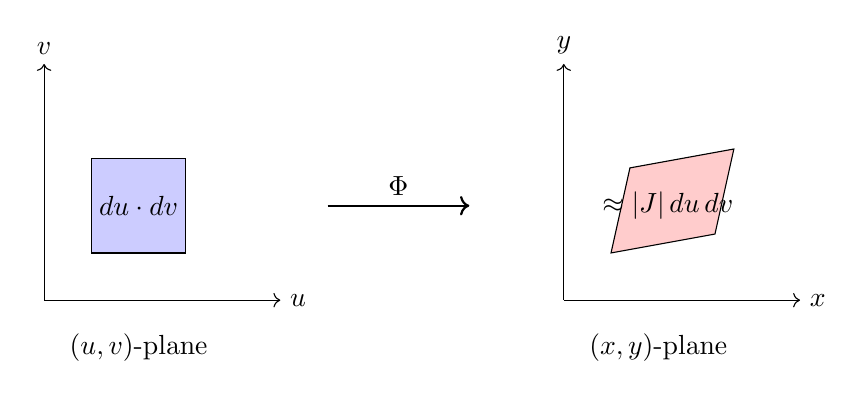
\begin{tikzpicture}[scale=1.2]
% Left: (u,v) plane
\draw[->] (0,0) -- (2.5,0) node[right] {$u$};
\draw[->] (0,0) -- (0,2.5) node[above] {$v$};
\draw[fill=blue!20] (0.5,0.5) rectangle (1.5,1.5);
\node at (1,1) {$du \cdot dv$};
\node at (1,-0.5) {$(u,v)$-plane};

% Arrow
\draw[->, thick] (3,1) -- (4.5,1) node[midway, above] {$\Phi$};

% Right: (x,y) plane
\begin{scope}[xshift=5.5cm]
\draw[->] (0,0) -- (2.5,0) node[right] {$x$};
\draw[->] (0,0) -- (0,2.5) node[above] {$y$};
\draw[fill=red!20] (0.5,0.5) -- (1.6,0.7) -- (1.8,1.6) -- (0.7,1.4) -- cycle;
\node at (1.1,1) {$\approx |J| \, du \, dv$};
\node at (1,-0.5) {$(x,y)$-plane};
\end{scope}
\end{tikzpicture}
\end{center}

To make the integral come out correctly, we must \textbf{compensate for this area distortion} by multiplying by $|J|$:
\[
\underbrace{\iint_D f(x, y) \, dx \, dy}_{\text{sum of } f \times \text{(true area)}} = \underbrace{\iint_{D^*} f(\Phi(u,v)) \cdot |J(u,v)| \, du \, dv}_{\text{sum of } f \times |J| \times du \, dv}
\]

The factor $|J|$ exactly cancels the area distortion, ensuring both sides compute the same weighted sum.

\medskip

\noindent\textbf{Section Organization:}
\begin{enumerate}
    \item \textbf{Preliminaries:} Jordan measurability and the 1D formula
    \item \textbf{Main Theorem:} Statement for rectangular domains, with three proofs
    \item \textbf{Extension:} General Jordan measurable domains
    \item \textbf{Geometric Interpretation:} Determinants as volume distortion; higher dimensions
    \item \textbf{Coordinate Systems and Worked Examples:} Polar, elliptical, spherical; full computations
\end{enumerate}

\subsection*{Preliminaries}

\begin{definition}[Jordan Measure Zero]
A bounded set $E \subseteq \R^2$ has \textbf{Jordan measure zero} if for every $\varepsilon > 0$, there exist finitely many rectangles $R_1, \ldots, R_N$ such that:
\[
E \subseteq \bigcup_{k=1}^N R_k \quad \text{and} \quad \sum_{k=1}^N \text{Area}(R_k) < \varepsilon.
\]
\end{definition}

\begin{definition}[Jordan Measurable Set]
A bounded set $D \subseteq \R^2$ is \textbf{Jordan measurable} if its boundary $\partial D$ has Jordan measure zero.
\end{definition}

\begin{example}[Jordan Measurable Sets]
The following are Jordan measurable:
\begin{itemize}
    \item Rectangles, triangles, and polygons
    \item Disks $\{(x,y): x^2 + y^2 \leq r^2\}$ and ellipses
    \item Type I regions: $\{(x,y): a \leq x \leq b, \, \phi(x) \leq y \leq \psi(x)\}$ where $\phi, \psi$ are continuous
    \item Type II regions: $\{(x,y): c \leq y \leq d, \, \phi(y) \leq x \leq \psi(y)\}$ where $\phi, \psi$ are continuous
    \item Finite unions and intersections of the above
\end{itemize}

\textbf{Non-example:} The set $\mathbb{Q}^2 \cap [0,1]^2$ (rationals in the unit square) is \textit{not} Jordan measurable --- its boundary is the entire square $[0,1]^2$.
\end{example}

\begin{lemma}[One-Dimensional Change of Variables]
\label{lem:1d-cov}
Let $g: [a, b] \to [\alpha, \beta]$ be a $C^1$ bijection with $g'(t) \neq 0$ throughout. If $f$ is continuous on $[\alpha, \beta]$, then:
\[
\int_\alpha^\beta f(x) \, dx = \int_a^b f(g(t)) \cdot |g'(t)| \, dt.
\]
\end{lemma}

\begin{proof}
Define $F(x) = \int_\alpha^x f(s) \, ds$, so $F'(x) = f(x)$ by the Fundamental Theorem of Calculus.

Consider the composition $H(t) = F(g(t))$. By the chain rule:
\[
H'(t) = F'(g(t)) \cdot g'(t) = f(g(t)) \cdot g'(t).
\]

Integrating from $a$ to $b$:
\[
H(b) - H(a) = \int_a^b f(g(t)) \cdot g'(t) \, dt.
\]

But $H(b) - H(a) = F(g(b)) - F(g(a))$.

If $g' > 0$: then $g(a) = \alpha$, $g(b) = \beta$, so $H(b) - H(a) = F(\beta) - F(\alpha) = \int_\alpha^\beta f(x) \, dx$.

If $g' < 0$: then $g(a) = \beta$, $g(b) = \alpha$, and the formula gives a negative sign that cancels with $|g'| = -g'$.
\end{proof}

\subsection*{Main Theorem (Rectangular Domain)}

\begin{theorem}[Change of Variables Formula --- Rectangular Case]
\label{thm:cov-rectangle}
Let $D^* = [a,b] \times [c,d]$ be a rectangle. Let $\Phi: D^* \to D$ be a $C^1$ bijection with $C^1$ inverse, where $D = \Phi(D^*)$.

Write $\Phi(u, v) = (\varphi(u, v), \psi(u, v)) = (x, y)$.

Assume the \textbf{Jacobian}
\[
J = \frac{\partial(x, y)}{\partial(u, v)} = \det \begin{pmatrix} \varphi_u & \varphi_v \\ \psi_u & \psi_v \end{pmatrix} = \varphi_u \psi_v - \varphi_v \psi_u
\]
satisfies $J \neq 0$ on $D^*$.

If $f$ is continuous on $\overline{D}$, then:
\[
\boxed{\iint_D f(x, y) \, dx \, dy = \iint_{D^*} f(\varphi(u, v), \psi(u, v)) \cdot |J(u, v)| \, du \, dv}
\]
\end{theorem}

We present three different proofs, each offering a distinct perspective:

\begin{center}
\renewcommand{\arraystretch}{1.4}
\begin{tabular}{|c|l|l|}
\hline
\textbf{Proof} & \textbf{Method} & \textbf{Key Idea} \\
\hline
1 & Linear Case + Taylor & Prove for linear maps, then linearize via Taylor \\
\hline
2 & Implicit Function Theorem & Reduce 2D to two 1D substitutions via IFT \\
\hline
3 & Two-Step Decomposition & Factor into primitive transformations \\
\hline
\end{tabular}
\end{center}

\medskip

\noindent\textbf{Proof 1} is the most geometric: it shows why the Jacobian determinant measures area distortion. \textbf{Proof 2} is the most analytic: it tracks coordinate changes explicitly. \textbf{Proof 3} (from Courant-John) generalizes most easily to $n$ dimensions.

\bigskip
\hrule
\bigskip

\begin{proof}[\textbf{First Proof: Linear Case + Taylor Linearization}]
We give a rigorous proof by first establishing the result for linear transformations, then extending to the general $C^1$ case with explicit error estimates.

\textbf{Part I: The Linear Case.}

Consider the linear transformation:
\[
\begin{pmatrix} x \\ y \end{pmatrix} = \begin{pmatrix} a & b \\ c & d \end{pmatrix} \begin{pmatrix} u \\ v \end{pmatrix}, \quad \text{i.e.,} \quad x = au + bv, \quad y = cu + dv.
\]

The Jacobian is $J = ad - bc$ (the determinant of the matrix).

\textit{Claim:} A rectangle $[u_0, u_0 + h] \times [v_0, v_0 + k]$ maps to a parallelogram with area $|J| \cdot hk$.

\textit{Proof of claim:} The four corners of the rectangle map to:
\begin{align*}
(u_0, v_0) &\mapsto (au_0 + bv_0, \, cu_0 + dv_0) =: P_0 \\
(u_0 + h, v_0) &\mapsto (au_0 + bv_0 + ah, \, cu_0 + dv_0 + ch) =: P_1 \\
(u_0, v_0 + k) &\mapsto (au_0 + bv_0 + bk, \, cu_0 + dv_0 + dk) =: P_2 \\
(u_0 + h, v_0 + k) &\mapsto (au_0 + bv_0 + ah + bk, \, cu_0 + dv_0 + ch + dk) =: P_3
\end{align*}

Observe that $\mathbf{P_0 P_1} = (ah, ch)$ and $\mathbf{P_0 P_2} = (bk, dk)$. Also, $\mathbf{P_2 P_3} = (ah, ch) = \mathbf{P_0 P_1}$ and $\mathbf{P_1 P_3} = (bk, dk) = \mathbf{P_0 P_2}$. Thus the image is indeed a parallelogram (opposite sides are equal and parallel).

The two edge vectors of the parallelogram are:
\[
\boldsymbol{\alpha} = (ah, ch), \quad \boldsymbol{\beta} = (bk, dk).
\]

The area of the parallelogram is $|\det(\boldsymbol{\alpha}, \boldsymbol{\beta})|$:
\[
\text{Area} = \left| \det \begin{pmatrix} ah & bk \\ ch & dk \end{pmatrix} \right| = |adhk - bchk| = |ad - bc| \cdot hk = |J| \cdot hk.
\]

\textbf{Part II: General Case $\varphi, \psi \in C^1(D^*)$.}

Now consider the general transformation $\Phi(u, v) = (\varphi(u, v), \psi(u, v))$ where $\varphi, \psi$ are $C^1$ on a compact domain $\overline{D^*}$.

Assume $J \neq 0$ on $D^*$ (WLOG, say $J > 0$; the case $J < 0$ is similar with $|J| = -J$).

\textbf{Step 1: Taylor expansion with explicit remainder.}

Fix a point $(u_0, v_0) \in D^*$. For $(u, v)$ near $(u_0, v_0)$, Taylor's theorem gives:
\begin{align*}
\varphi(u, v) &= \varphi(u_0, v_0) + \varphi_u(u_0, v_0)(u - u_0) + \varphi_v(u_0, v_0)(v - v_0) + R_\varphi(u, v) \\
\psi(u, v) &= \psi(u_0, v_0) + \psi_u(u_0, v_0)(u - u_0) + \psi_v(u_0, v_0)(v - v_0) + R_\psi(u, v)
\end{align*}
where the remainders satisfy:
\[
|R_\varphi(u, v)|, |R_\psi(u, v)| \leq M \cdot \|(u - u_0, v - v_0)\|^2
\]
for some constant $M$ depending on bounds for the second derivatives of $\varphi, \psi$.

\textbf{Step 2: Image of a small rectangle.}

Consider the rectangle $R = [u_0, u_0 + h] \times [v_0, v_0 + k]$. Define the \textbf{linearized map} at $(u_0, v_0)$:
\[
L(u, v) = \Phi(u_0, v_0) + J_\Phi(u_0, v_0) \cdot \begin{pmatrix} u - u_0 \\ v - v_0 \end{pmatrix}
\]
where $J_\Phi = \begin{pmatrix} \varphi_u & \varphi_v \\ \psi_u & \psi_v \end{pmatrix}$ is the Jacobian matrix.

By Part I, the linearized map $L$ takes $R$ to a parallelogram $P$ with:
\[
\text{Area}(P) = |J(u_0, v_0)| \cdot hk.
\]

\textbf{Step 3: Rigorous error estimate for curvilinear vs.\ parallelogram area.}

The actual image $\Phi(R)$ is a curvilinear quadrilateral. We need to show the area differs from the parallelogram area by a controllable amount.

\textit{Setup:} Divide $D^*$ into small squares of side $1/2^m$. The number of squares is $2^k \cdot 2^k = 2^{2k}$ for some $k$.

Since $\varphi, \psi \in C^1(\overline{D^*})$, the functions $\varphi, \psi, \varphi_u, \varphi_v, \psi_u, \psi_v$ are all uniformly continuous on the compact domain. Also, assume these are bounded by some constant $B$:
\[
|\varphi_u|, |\varphi_v|, |\psi_u|, |\psi_v|, |\varphi|, |\psi| \leq B.
\]

\textit{Focus on one small square:} Consider the square $[u_0, u_0 + h] \times [v_0, v_0 + k]$ where $h = k = 1/2^m$.

A point $(u_0 + \theta h, v_0 + \alpha k)$ in this square (with $\theta, \alpha \in [0,1]$) maps to:
\[
\Phi(u_0 + \theta h, v_0 + \alpha k) = (\varphi(u_0 + \theta h, v_0 + \alpha k), \, \psi(u_0 + \theta h, v_0 + \alpha k)).
\]

The displacement from the corner $\Phi(u_0, v_0)$ is:
\begin{align*}
&\Phi(u_0 + \theta h, v_0 + \alpha k) - \Phi(u_0, v_0) \\
&= \big( \varphi(u_0 + \theta h, v_0 + \alpha k) - \varphi(u_0, v_0), \; \psi(u_0 + \theta h, v_0 + \alpha k) - \psi(u_0, v_0) \big).
\end{align*}

\textit{Linear approximation:} By the Mean Value Theorem:
\begin{align*}
\varphi(u_0 + \theta h, v_0 + \alpha k) - \varphi(u_0, v_0) &= \varphi_u(u_0 + \theta' h, v_0 + \alpha' k) \cdot \theta h + \varphi_v(u_0 + \theta'' h, v_0 + \alpha'' k) \cdot \alpha k
\end{align*}
for some intermediate points.

The \textbf{linearized approximation} at $(u_0, v_0)$ would give:
\[
\varphi_u(u_0, v_0) \cdot \theta h + \varphi_v(u_0, v_0) \cdot \alpha k.
\]

\textit{Error in first component:}
\begin{align*}
|\text{error}_1| &= \big| \varphi_u(u_0 + \theta' h, v_0 + \alpha' k) - \varphi_u(u_0, v_0) \big| \cdot h \\
&\quad + \big| \varphi_v(u_0 + \theta'' h, v_0 + \alpha'' k) - \varphi_v(u_0, v_0) \big| \cdot k.
\end{align*}

\textit{Using uniform continuity:} For any $\varepsilon > 0$, there exists $M$ such that for all $m \geq M$:
\[
\sup_{D_{ij}} \varphi_u - \inf_{D_{ij}} \varphi_u \leq \varepsilon
\]
where $D_{ij}$ is any square of side $1/2^m$. The same holds for $\varphi_v, \psi_u, \psi_v$ (six versions of $M$: $M_1, M_2, \ldots$; take $M = \max$).

Therefore, for $m \geq M$:
\[
|\text{error}_1| \leq \varepsilon \cdot \frac{1}{2^m} + \varepsilon \cdot \frac{1}{2^m} = \frac{2\varepsilon}{2^m}.
\]

Similarly, $|\text{error}_2| \leq \frac{2\varepsilon}{2^m}$.

\textit{Total position error:}
\[
|\text{error}| \leq \sqrt{(\text{error}_1)^2 + (\text{error}_2)^2} \leq \sqrt{4\varepsilon^2 \cdot \frac{1}{2^{2m}} + 4\varepsilon^2 \cdot \frac{1}{2^{2m}}} = \sqrt{2} \cdot \frac{2\varepsilon}{2^m}.
\]

\textit{Geometric interpretation:} For each point in the parallelogram (the linearized image), draw a ball of radius $r = 2\sqrt{2} \varepsilon / 2^m$. The actual image point lies inside this ball.

Take the union: $\bigcup_{p \in \text{parallelogram}} B(p; 2\sqrt{2}\varepsilon/2^m)$.

\textit{Area error estimate:} Assume the error region remains on the same side (no self-intersection, guaranteed when $\varepsilon$ is small relative to $|J|$). The error region is like a ``fattened boundary'' of the parallelogram.

\begin{itemize}
    \item The parallelogram has perimeter $\leq 4B \cdot (h + k) = 8B/2^m$ (since edge vectors have length $\leq B \cdot h$ and $B \cdot k$).
    \item Fattening by radius $r = 2\sqrt{2}\varepsilon/2^m$ adds area $\leq \text{perimeter} \times r + \pi r^2$.
\end{itemize}

Therefore:
\[
|\text{Area}(\Phi(R)) - \text{Area}(P)| \leq \frac{8B}{2^m} \cdot \frac{2\sqrt{2}\varepsilon}{2^m} + \pi \left( \frac{2\sqrt{2}\varepsilon}{2^m} \right)^2 = O\left( \frac{\varepsilon}{2^{2m}} \right).
\]

Since Area$(P) = |J| \cdot h \cdot k = |J|/2^{2m}$, the relative error is $O(\varepsilon)$, which can be made arbitrarily small.

\textbf{Step 4: Riemann sum estimate.}

Partition $D^*$ into $N = 2^{2m}$ small squares $R_{ij}$ of side $\Delta = 1/2^m$.

Let $(u_{ij}, v_{ij})$ be a point in $R_{ij}$, and let $(x_{ij}, y_{ij}) = \Phi(u_{ij}, v_{ij})$.

The Riemann sum for $\iint_D f \, dA$ is:
\[
S_N := \sum_{i,j} f(x_{ij}, y_{ij}) \cdot \text{Area}(\Phi(R_{ij})).
\]

By Step 3:
\[
\text{Area}(\Phi(R_{ij})) = |J(u_{ij}, v_{ij})| \cdot \Delta^2 + E_{ij}
\]
where $|E_{ij}| \leq C \varepsilon \cdot \Delta^2$ for $m \geq M(\varepsilon)$.

Therefore:
\[
S_N = \sum_{i,j} f(x_{ij}, y_{ij}) \cdot |J(u_{ij}, v_{ij})| \cdot \Delta^2 + \sum_{i,j} f(x_{ij}, y_{ij}) \cdot E_{ij}.
\]

\textbf{Step 5: Error vanishes in the limit.}

Since $f$ is continuous on the compact set $\overline{D}$, it is bounded: $|f| \leq M_f$.

The total error is:
\[
\left| \sum_{i,j} f(x_{ij}, y_{ij}) \cdot E_{ij} \right| \leq M_f \cdot \sum_{i,j} |E_{ij}| \leq M_f \cdot C\varepsilon \sum_{i,j} \Delta^2 = M_f \cdot C\varepsilon \cdot \text{Area}(D^*).
\]

Since $\varepsilon > 0$ was arbitrary, this error can be made as small as desired by choosing $m$ large enough.

\textbf{Step 6: Transition from finite sum to integral (Riemann sum argument).}

Cut the domain $D^*$ into $(2^m)^2$ pieces. Label all squares as $D_{ij}^{(m)}$ for $1 \leq i, j \leq 2^m$.

After being mapped by $(\varphi, \psi)$, the square $D_{ij}^{(m)}$ maps to a curvilinear region $\Sigma_{ij}^{(m)}$.

Denote the parallelogram approximation of $\Sigma_{ij}^{(m)}$ as $S_{ij}^{(m)}$.

By Step 5, for all $\varepsilon > 0$, there exists $M$ such that for all $m \geq M$:
\[
\sum_{i=1}^{2^m} \sum_{j=1}^{2^m} \big| |\Sigma_{ij}^{(m)}| - |S_{ij}^{(m)}| \big| \leq C\varepsilon
\]
for some constant $C$ depending only on the bound $B$ for the partial derivatives.

Now we relate the two sums:

\textit{Exact area sum:}
\[
\sum_{i,j} |\Sigma_{ij}^{(m)}| = |\Sigma| = \text{Area}(D) = \iint_D dx \, dy.
\]

\textit{Parallelogram approximation sum:}
\[
\sum_{i,j} |S_{ij}^{(m)}| = \sum_{i,j} \left| \det \begin{pmatrix} \varphi_u & \varphi_v \\ \psi_u & \psi_v \end{pmatrix}_{(u_{i-1}, v_{j-1})} \right| \cdot \left( \frac{1}{2^m} \right)^2 = \sum_{i,j} |J(u_{i-1}, v_{j-1})| \cdot \left( \frac{1}{2^m} \right)^2.
\]

This is a Riemann sum for $\iint_{D^*} |J| \, du \, dv$.

As $m \to \infty$, the Riemann sum converges:
\[
\sum_{i,j} |S_{ij}^{(m)}| = \sum_{i,j} |J(u_{i-1}, v_{j-1})| \cdot \left( \frac{1}{2^m} \right)^2 \xrightarrow{m \to \infty} \iint_{D^*} |J| \, du \, dv.
\]

Since $\big| \sum_{i,j} |\Sigma_{ij}^{(m)}| - \sum_{i,j} |S_{ij}^{(m)}| \big| \leq C\varepsilon$ for $m \geq M$, and $\varepsilon$ was arbitrary:
\[
\iint_D dx \, dy = |\Sigma| = \iint_{D^*} |J| \, du \, dv.
\]

\textbf{Step 7: Derive the final result with $f$.}

Now consider $\iint_D f(x, y) \, dx \, dy$.

The ``diameter'' of the curvilinear region $\Sigma_{ij}^{(m)}$ is:
\[
\text{diam}(\Sigma_{ij}^{(m)}) = \sqrt{(\varphi(u_i, v_j) - \varphi(u_{i-1}, v_{j-1}))^2 + (\psi(u_i, v_j) - \psi(u_{i-1}, v_{j-1}))^2} \leq CB \cdot \sqrt{(u_i - u_{i-1})^2 + (v_j - v_{j-1})^2}
\]
for some constant $C$ depending on the bounds of the partial derivatives.

As $m \to \infty$, the diameter $\to 0$, so by the definition of the Riemann integral:
\[
\iint_D f(x, y) \, dx \, dy = \lim_{m \to \infty} \sum_{i,j} f(x_{ij}^*, y_{ij}^*) \cdot |\Sigma_{ij}^{(m)}|
\]
where $(x_{ij}^*, y_{ij}^*)$ is any point in $\Sigma_{ij}^{(m)}$.

Choose $(x_{ij}^*, y_{ij}^*) = (\varphi(u_{i-1}, v_{j-1}), \psi(u_{i-1}, v_{j-1}))$. Then:
\begin{align*}
\iint_D f(x, y) \, dx \, dy &= \lim_{m \to \infty} \sum_{i,j} f(\varphi(u_{i-1}, v_{j-1}), \psi(u_{i-1}, v_{j-1})) \cdot |\Sigma_{ij}^{(m)}| \\
&= \lim_{m \to \infty} \sum_{i,j} f(\varphi(u_{i-1}, v_{j-1}), \psi(u_{i-1}, v_{j-1})) \cdot |J(u_{i-1}, v_{j-1})| \cdot \frac{1}{(2^m)^2} \\
&= \iint_{D^*} f(\varphi(u, v), \psi(u, v)) \cdot |J(u, v)| \, du \, dv.
\end{align*}

The second equality uses that $|\Sigma_{ij}^{(m)}| = |J| \cdot (1/2^m)^2 + O(\varepsilon/2^{2m})$ and the error vanishes in the limit (since $f$ is bounded and the total error is $O(\varepsilon)$).

This completes the proof for the case where $D^*$ is a square. \qedhere
\end{proof}

\begin{remark}[Extension to Arbitrary Domains: Jordan Measurability]
The proof above assumes $D^*$ is a square (or rectangle). For arbitrary domains, we need additional assumptions and a more careful treatment using \textbf{Jordan measure}.

\textbf{The Problem:} If $D^*$ is not a rectangle, how do we define the Riemann sum? We can't simply partition $D^*$ into small squares --- some squares will partially overlap the boundary $\partial D^*$.

\textbf{Solution: Jordan Measurable Domains.}

\textit{Definition:} A bounded set $D^* \subseteq \R^2$ is \textbf{Jordan measurable} if its boundary $\partial D^*$ has Jordan measure zero, i.e., for any $\varepsilon > 0$, the boundary can be covered by finitely many rectangles with total area $< \varepsilon$.

\textit{Equivalently:} The \textbf{inner Jordan measure} (supremum of areas of finite unions of rectangles contained in $D^*$) equals the \textbf{outer Jordan measure} (infimum of areas of finite unions of rectangles containing $D^*$).

\textbf{Procedure for Arbitrary Jordan Measurable $D^*$:}

\textit{Step 1:} Enclose $D^*$ in a large rectangle $R = [a, b] \times [c, d]$.

\textit{Step 2:} Partition $R$ into small squares of side $1/2^m$. Classify each square $D_{ij}^{(m)}$ as:
\begin{itemize}
    \item \textbf{Interior squares:} $D_{ij}^{(m)} \subseteq D^*$ (entirely inside)
    \item \textbf{Exterior squares:} $D_{ij}^{(m)} \cap D^* = \emptyset$ (entirely outside)
    \item \textbf{Boundary squares:} $D_{ij}^{(m)} \cap \partial D^* \neq \emptyset$ (touch the boundary)
\end{itemize}

\textit{Step 3:} For the Riemann sum, sum only over interior squares:
\[
S_m^{\text{inner}} = \sum_{\substack{i,j \\ D_{ij}^{(m)} \subseteq D^*}} f(\varphi(u_{ij}), \psi(u_{ij})) \cdot |J(u_{ij})| \cdot \frac{1}{(2^m)^2}.
\]

Similarly, define the outer sum including boundary squares.

\textit{Step 4:} Since $\partial D^*$ has Jordan measure zero:
\[
\#\{\text{boundary squares}\} \cdot \frac{1}{(2^m)^2} \to 0 \quad \text{as } m \to \infty.
\]

Therefore, inner and outer sums converge to the same limit.

\textbf{Additional Assumption Needed:}

For the Change of Variables formula, we need both $D^*$ and $D = \Phi(D^*)$ to be Jordan measurable.

\textit{Key Lemma:} If $D^*$ is Jordan measurable and $\Phi: D^* \to D$ is a $C^1$ diffeomorphism with $J \neq 0$, then $D = \Phi(D^*)$ is also Jordan measurable.

\textit{Proof sketch:} The boundary $\partial D = \Phi(\partial D^*)$. Since $\Phi$ is $C^1$ and $\partial D^*$ has measure zero, the image $\Phi(\partial D^*)$ also has measure zero (Lipschitz maps preserve measure zero sets). \hfill $\square$

\textbf{Refined Theorem Statement:}

\begin{quote}
Let $D^* \subseteq \R^2$ be a \textbf{bounded, Jordan measurable} domain. Let $\Phi: \overline{D^*} \to \overline{D}$ be a $C^1$ bijection with $C^1$ inverse and $J \neq 0$ on $D^*$. If $f$ is continuous on $\overline{D}$, then:
\[
\iint_D f(x, y) \, dx \, dy = \iint_{D^*} f(\varphi(u, v), \psi(u, v)) \cdot |J(u, v)| \, du \, dv.
\]
\end{quote}

\textbf{Common Jordan Measurable Domains:}
\begin{itemize}
    \item Rectangles, triangles, polygons
    \item Disks, ellipses
    \item Regions bounded by $C^1$ curves (Type I and Type II regions)
    \item Finite unions and intersections of the above
\end{itemize}

\textbf{Non-Example:} The set of points in $[0,1]^2$ with both coordinates rational is bounded but \textit{not} Jordan measurable (its boundary is the entire square, which has positive area).
\end{remark}

\begin{remark}[Alternative: Lebesgue Integration]
In Lebesgue integration theory (MATH 551), the situation is cleaner:
\begin{itemize}
    \item The change of variables formula holds for any \textbf{Lebesgue measurable} set $D^*$.
    \item No need for Jordan measurability --- Lebesgue measure handles much more general sets.
    \item The assumption ``$J \neq 0$ everywhere'' can be relaxed to ``$J \neq 0$ almost everywhere.''
\end{itemize}

However, for this course (Riemann integration), Jordan measurability is the appropriate condition.
\end{remark}

\bigskip
\hrule
\bigskip

\begin{proof}[\textbf{Second Proof: Implicit Function Theorem Approach}]
This approach uses IFT to introduce intermediate coordinates $(x, v)$, reducing the 2D change of variables to two applications of the 1D formula (Lemma~\ref{lem:1d-cov}).

\textbf{Setup and Assumptions.}

Consider the transformation $\Phi(u, v) = (\varphi(u, v), \psi(u, v))$ with Jacobian $J = \varphi_u \psi_v - \varphi_v \psi_u$.

Since $J \neq 0$ and the partial derivatives are continuous, at least one of $\varphi_u$ or $\varphi_v$ is nonzero at each point. WLOG, assume $\varphi_u > 0$ throughout (if not, we can partition the domain or relabel variables).

Also assume $J > 0$ (the case $J < 0$ gives $|J| = -J$).

\textbf{Step 1: Apply IFT to introduce $(x, v)$ coordinates.}

Define $F(u, v, x) = \varphi(u, v) - x$. Since $F_u = \varphi_u > 0$, by the Implicit Function Theorem, we can locally solve $F = 0$ for $u$:
\[
\exists \, u = U(x, v) \quad \text{such that} \quad \varphi(U(x, v), v) = x.
\]

The function $U$ is $C^1$ with derivatives computed by implicit differentiation. Differentiating $\varphi(U(x,v), v) = x$:
\begin{align*}
\text{w.r.t. } x: \quad & \varphi_u \cdot U_x = 1 \quad \Longrightarrow \quad U_x = \frac{1}{\varphi_u} > 0. \\
\text{w.r.t. } v: \quad & \varphi_u \cdot U_v + \varphi_v = 0 \quad \Longrightarrow \quad U_v = -\frac{\varphi_v}{\varphi_u}.
\end{align*}

\textbf{Step 2: Define $\gamma(x, v)$ and compute its derivative.}

Define the composed function:
\[
\gamma(x, v) := \psi(U(x, v), v).
\]

This gives $y$ as a function of $(x, v)$: when we hold $x$ fixed and vary $v$, the point $(x, y) = (x, \gamma(x, v))$ traces a curve in the $(x, y)$-plane.

Compute $\gamma_v$ using the chain rule:
\begin{align*}
\gamma_v &= \psi_u \cdot U_v + \psi_v = \psi_u \cdot \left( -\frac{\varphi_v}{\varphi_u} \right) + \psi_v \\
&= \frac{-\psi_u \varphi_v + \psi_v \varphi_u}{\varphi_u} = \frac{\varphi_u \psi_v - \varphi_v \psi_u}{\varphi_u} = \frac{J}{\varphi_u} > 0.
\end{align*}

The inequality $\gamma_v > 0$ shows that, for fixed $x$, the map $v \mapsto y = \gamma(x, v)$ is strictly increasing.

\textbf{Step 3: Change variables $(x, y) \to (x, v)$ using the 1D formula.}

Consider any region $R$ in the $(x, y)$-plane that is the image of a region $B$ in the $(x, v)$-plane under the map $(x, v) \mapsto (x, \gamma(x, v))$.

For fixed $x$, the map $v \mapsto y = \gamma(x, v)$ satisfies $\frac{dy}{dv} = \gamma_v(x, v)$.

By the 1D change of variables formula (Lemma~\ref{lem:1d-cov}) applied to the inner integral:
\[
\int_{y_1(x)}^{y_2(x)} f(x, y) \, dy = \int_{v_1}^{v_2} f(x, \gamma(x, v)) \cdot \gamma_v(x, v) \, dv.
\]

Integrating over $x$ and using Fubini:
\[
\iint_R f(x, y) \, dx \, dy = \iint_B f(x, \gamma(x, v)) \cdot \gamma_v(x, v) \, dx \, dv = \iint_B f(x, y) \cdot \frac{J}{\varphi_u} \, dx \, dv.
\]

\textbf{Step 4: Change variables $(x, v) \to (u, v)$ using the 1D formula again.}

Now we transform from $(x, v)$ to $(u, v)$ via $x = \varphi(u, v)$, $v = v$.

For fixed $v$, the map $u \mapsto x = \varphi(u, v)$ satisfies $\frac{dx}{du} = \varphi_u(u, v) > 0$.

By the 1D formula applied to the inner integral (now integrating over $x$):
\[
\int_{x_1(v)}^{x_2(v)} g(x, v) \, dx = \int_{u_1}^{u_2} g(\varphi(u, v), v) \cdot \varphi_u(u, v) \, du.
\]

Applying this to our integral with $g(x, v) = f(x, \gamma(x, v)) \cdot \frac{J}{\varphi_u}$:
\[
\iint_B f(x, y) \cdot \frac{J}{\varphi_u} \, dx \, dv = \iint_{D^*} f(\varphi, \psi) \cdot \frac{J(u,v)}{\varphi_u(u,v)} \cdot \varphi_u(u, v) \, du \, dv.
\]

The $\varphi_u$ terms cancel:
\[
\iint_R f(x, y) \, dx \, dy = \iint_{D^*} f(\varphi(u, v), \psi(u, v)) \cdot J(u, v) \, du \, dv.
\]

Since we assumed $J > 0$, we have $J = |J|$, completing the proof.
\end{proof}

\bigskip
\hrule
\bigskip

\begin{proof}[\textbf{Third Proof: Two-Step Decomposition (Courant-John)}]
This approach, from Courant \& John's \textit{Introduction to Calculus and Analysis}, decomposes the general transformation into two simpler ``primitive'' transformations, each changing only one variable at a time. This method extends naturally to higher dimensions.

\textbf{Setup.} We want to prove:
\[
\iint_R f(x, y) \, dx \, dy = \iint_{R'} f(\phi(u, v), \psi(u, v)) \left| \frac{\partial(x, y)}{\partial(u, v)} \right| du \, dv
\]
where $x = \phi(u, v)$, $y = \psi(u, v)$ gives a 1-1 $C^1$ mapping of region $R$ onto region $R'$ with $J \neq 0$.

\textbf{Key Idea: Factor the transformation into two primitive steps.}

A \textbf{primitive transformation} is one that changes only one coordinate:
\begin{itemize}
    \item Type I: $(x, v) \mapsto (x, y)$ where $x$ stays fixed, $y = \Phi(v, x)$
    \item Type II: $(u, v) \mapsto (x, v)$ where $v$ stays fixed, $x = \Psi(u, v)$
\end{itemize}

\textit{Claim:} Any $C^1$ transformation with $J \neq 0$ can be locally decomposed as a composition of two primitive transformations.

\textit{Proof of claim:} Since $J = \phi_u \psi_v - \phi_v \psi_u \neq 0$, at least one of $\phi_u$ or $\phi_v$ is nonzero. 

\textbf{Case 1:} If $\phi_u \neq 0$, define:
\begin{align*}
\text{Step 2: } & (u, v) \mapsto (x, v) \quad \text{via} \quad x = \phi(u, v), \; v = v \\
\text{Step 1: } & (x, v) \mapsto (x, y) \quad \text{via} \quad x = x, \; y = \psi(U(x, v), v)
\end{align*}
where $U(x, v)$ is the inverse of $u \mapsto \phi(u, v)$ for fixed $v$ (exists by IFT since $\phi_u \neq 0$).

\textbf{Case 2:} If $\phi_v \neq 0$, we can interchange $u$ and $v$ and proceed similarly.

In either case, the region $R$ can be covered by finitely many subregions where the decomposition works, and the integral over $R$ is the sum of integrals over these subregions. \hfill $\square$ (claim)

\textbf{Primitive Transformation Formula.}

We prove the change of variables formula for primitive transformations using the 1D result (Lemma~\ref{lem:1d-cov}).

Consider a Type I primitive: $(x, v) \mapsto (x, y)$ with $y = \Phi(v, x)$ and $\Phi_v > 0$.

For fixed $x$, the map $v \mapsto y = \Phi(v, x)$ is a 1D change of variables with derivative $\Phi_v$.

By Lemma~\ref{lem:1d-cov}:
\[
\int_{y_1}^{y_2} f(x, y) \, dy = \int_{v_1}^{v_2} f(x, \Phi(v, x)) \cdot \Phi_v(v, x) \, dv.
\]

Integrating over $x$ and using Fubini:
\[
\iint_R f(x, y) \, dx \, dy = \iint_B f(x, \Phi(v, x)) \cdot \Phi_v(v, x) \, dx \, dv.
\]

The Jacobian of the Type I primitive is:
\[
\frac{\partial(x, y)}{\partial(x, v)} = \det \begin{pmatrix} 1 & 0 \\ \Phi_x & \Phi_v \end{pmatrix} = \Phi_v.
\]

Similarly, for a Type II primitive $(u, v) \mapsto (x, v)$ with $x = \Psi(u, v)$ and $\Psi_u > 0$:
\[
\iint_B g(x, v) \, dx \, dv = \iint_{R'} g(\Psi(u, v), v) \cdot \Psi_u(u, v) \, du \, dv.
\]

The Jacobian is:
\[
\frac{\partial(x, v)}{\partial(u, v)} = \det \begin{pmatrix} \Psi_u & \Psi_v \\ 0 & 1 \end{pmatrix} = \Psi_u.
\]

\textbf{Combining the Two Steps.}

Composing the two primitive transformations $(u, v) \xrightarrow{\text{II}} (x, v) \xrightarrow{\text{I}} (x, y)$:

\textit{Step 1 (Type II):}
\[
\iint_B f(x, \Phi(v, x)) \cdot \Phi_v \, dx \, dv = \iint_{R'} f(\Psi, \Phi(v, \Psi)) \cdot \Phi_v(v, \Psi) \cdot \Psi_u \, du \, dv.
\]

Note that $y = \Phi(v, \Psi(u, v)) = \psi(u, v)$ by construction.

\textit{Step 2 (Chain Rule for Jacobians):}
\[
\frac{\partial(x, y)}{\partial(u, v)} = \frac{\partial(x, y)}{\partial(x, v)} \cdot \frac{\partial(x, v)}{\partial(u, v)} = \Phi_v \cdot \Psi_u.
\]

\textbf{Conclusion.}

Combining everything:
\[
\iint_R f(x, y) \, dx \, dy = \iint_{R'} f(\phi(u, v), \psi(u, v)) \cdot \Phi_v \cdot \Psi_u \, du \, dv = \iint_{R'} f(\phi, \psi) \left| \frac{\partial(x, y)}{\partial(u, v)} \right| du \, dv.
\]

(The absolute value appears because if $\Phi_v < 0$ or $\Psi_u < 0$, the orientation reverses, but the area element remains positive.)
\end{proof}

\begin{remark}[$|J|$ vs.\ $J$: Orientation and Area]
The change of variables formula uses $|J|$, not $J$. This distinction matters:
\begin{itemize}
    \item $|J|$ measures \textbf{area distortion}: how much the transformation stretches or compresses infinitesimal areas. This is always nonneg\-ative and is the correct factor for computing integrals.
    \item $J$ (with sign) measures \textbf{oriented area distortion}: $J > 0$ means the transformation preserves orientation, $J < 0$ means it reverses orientation (like a reflection).
\end{itemize}

A common exam mistake is writing $J$ instead of $|J|$ in the formula. If you know $J > 0$ on your domain (e.g., polar coordinates with $J = r > 0$ for $r > 0$), then $|J| = J$ and the distinction is harmless. But if orientation could reverse (e.g., a transformation involving a reflection), omitting the absolute value gives the wrong answer.

The signed Jacobian becomes important later when we study \textbf{differential forms} and \textbf{oriented integrals}, where the orientation of the domain carries geometric meaning.
\end{remark}

\subsection*{Extension to General Domains}

The proofs above assume $D^*$ is a rectangle. We now extend to arbitrary Jordan measurable domains.

\begin{proposition}[Boundary Squares Have Vanishing Total Area]
\label{prop:boundary-squares}
Let $D \subseteq \R^2$ be a bounded Jordan measurable set. Enclose $D$ in a rectangle $R$ and partition $R$ into $N^2$ squares of side $1/N$. Let $B_N$ denote the set of \textbf{boundary squares} (those that intersect $\partial D$).

Then:
\[
\lim_{N \to \infty} \#(B_N) \cdot \frac{1}{N^2} = 0.
\]
\end{proposition}

\begin{proof}
Since $D$ is Jordan measurable, $\partial D$ has Jordan measure zero. Thus for any $\varepsilon > 0$, there exist finitely many rectangles $R_1, \ldots, R_K$ with:
\[
\partial D \subseteq \bigcup_{k=1}^K R_k \quad \text{and} \quad \sum_{k=1}^K \text{Area}(R_k) < \varepsilon.
\]

A boundary square $S$ satisfies $S \cap \partial D \neq \emptyset$, so $S$ must intersect at least one $R_k$.

For $N$ large enough (specifically, $1/N$ smaller than the minimum side length of the $R_k$'s), each $R_k$ can intersect at most $C \cdot N^2 \cdot \text{Area}(R_k)$ squares of side $1/N$, where $C$ is a universal constant.

Therefore:
\[
\#(B_N) \leq C \cdot N^2 \cdot \sum_{k=1}^K \text{Area}(R_k) < C \cdot N^2 \cdot \varepsilon.
\]

Hence:
\[
\#(B_N) \cdot \frac{1}{N^2} < C \cdot \varepsilon.
\]

Since $\varepsilon > 0$ was arbitrary, the limit is zero.
\end{proof}

\begin{proposition}[$C^1$ Diffeomorphisms Preserve Jordan Measurability]
\label{prop:diffeo-jordan}
Let $D^* \subseteq \R^2$ be bounded and Jordan measurable. Let $\Phi: \overline{D^*} \to \R^2$ be a $C^1$ map. Then $\Phi(\partial D^*)$ has Jordan measure zero.

In particular, if $\Phi$ is a $C^1$ diffeomorphism onto $D = \Phi(D^*)$, then $D$ is Jordan measurable.
\end{proposition}

\begin{proof}
Since $\Phi$ is $C^1$ on the compact set $\overline{D^*}$, it is Lipschitz: there exists $L > 0$ such that
\[
\|\Phi(p) - \Phi(q)\| \leq L \|p - q\| \quad \text{for all } p, q \in \overline{D^*}.
\]

Let $\varepsilon > 0$. Since $\partial D^*$ has Jordan measure zero, there exist rectangles $R_1, \ldots, R_K$ with:
\[
\partial D^* \subseteq \bigcup_{k=1}^K R_k \quad \text{and} \quad \sum_{k=1}^K \text{Area}(R_k) < \frac{\varepsilon}{L^2}.
\]

For each rectangle $R_k$ with side lengths $a_k \times b_k$, the image $\Phi(R_k \cap \overline{D^*})$ is contained in a rectangle of side lengths at most $L \cdot a_k \times L \cdot b_k$ (since $\Phi$ stretches distances by at most $L$).

Therefore:
\[
\Phi(\partial D^*) \subseteq \bigcup_{k=1}^K \Phi(R_k \cap \overline{D^*}) \subseteq \bigcup_{k=1}^K \tilde{R}_k
\]
where $\text{Area}(\tilde{R}_k) \leq L^2 \cdot \text{Area}(R_k)$.

Hence:
\[
\sum_{k=1}^K \text{Area}(\tilde{R}_k) \leq L^2 \sum_{k=1}^K \text{Area}(R_k) < L^2 \cdot \frac{\varepsilon}{L^2} = \varepsilon.
\]

Since $\partial D = \Phi(\partial D^*)$ (for a bijection), this shows $\partial D$ has Jordan measure zero, so $D$ is Jordan measurable.
\end{proof}

\begin{theorem}[Change of Variables --- General Jordan Measurable Domains]
\label{thm:cov-general}
Let $D^* \subseteq \R^2$ be bounded and Jordan measurable. Let $\Phi: \overline{D^*} \to \overline{D}$ be a $C^1$ bijection with $C^1$ inverse, where $D = \Phi(D^*)$.

Write $\Phi(u, v) = (\varphi(u, v), \psi(u, v)) = (x, y)$, and assume $J = \varphi_u \psi_v - \varphi_v \psi_u \neq 0$ on $D^*$.

If $f$ is continuous on $\overline{D}$, then:
\[
\boxed{\iint_D f(x, y) \, dx \, dy = \iint_{D^*} f(\varphi(u, v), \psi(u, v)) \cdot |J(u, v)| \, du \, dv}
\]
\end{theorem}

\begin{proof}
Enclose $D^*$ in a rectangle $R^* = [a, b] \times [c, d]$. Partition $R^*$ into squares of side $\Delta = 1/2^m$. Classify each square $S_{ij}$ as:
\begin{itemize}
    \item \textbf{Interior:} $S_{ij} \subseteq D^*$
    \item \textbf{Exterior:} $S_{ij} \cap D^* = \emptyset$
    \item \textbf{Boundary:} $S_{ij} \cap \partial D^* \neq \emptyset$ and $S_{ij} \cap D^* \neq \emptyset$
\end{itemize}

Define the inner and outer Riemann sums:
\begin{align*}
S_m^{\text{inner}} &= \sum_{\text{interior } S_{ij}} f(\varphi(u_{ij}), \psi(u_{ij})) \cdot |J(u_{ij})| \cdot \Delta^2, \\
S_m^{\text{outer}} &= \sum_{\text{interior or boundary } S_{ij}} f(\varphi(u_{ij}), \psi(u_{ij})) \cdot |J(u_{ij})| \cdot \Delta^2.
\end{align*}

Since $f \circ \Phi$ and $|J|$ are continuous on $\overline{D^*}$, they are bounded: $|f \circ \Phi| \leq M_f$ and $|J| \leq M_J$.

The difference between outer and inner sums is:
\[
|S_m^{\text{outer}} - S_m^{\text{inner}}| \leq M_f \cdot M_J \cdot \#(\text{boundary squares}) \cdot \Delta^2.
\]

By Proposition~\ref{prop:boundary-squares}, this tends to zero as $m \to \infty$.

For interior squares, the proof of Theorem~\ref{thm:cov-rectangle} applies verbatim: each interior square maps to a curvilinear region with area $|J| \cdot \Delta^2 + O(\varepsilon \cdot \Delta^2)$.

Therefore, both $S_m^{\text{inner}}$ and $S_m^{\text{outer}}$ converge to the same limit:
\[
\lim_{m \to \infty} S_m^{\text{inner}} = \lim_{m \to \infty} S_m^{\text{outer}} = \iint_{D^*} f(\varphi, \psi) \cdot |J| \, du \, dv.
\]

On the other side, the same argument for the images (using that $D$ is Jordan measurable by Proposition~\ref{prop:diffeo-jordan}) shows:
\[
\iint_D f(x, y) \, dx \, dy = \lim_{m \to \infty} \sum_{\text{interior } \Sigma_{ij}} f(x_{ij}, y_{ij}) \cdot \text{Area}(\Sigma_{ij})
\]
where $\Sigma_{ij} = \Phi(S_{ij})$.

Since $\text{Area}(\Sigma_{ij}) = |J(u_{ij})| \cdot \Delta^2 + O(\varepsilon \cdot \Delta^2)$ by the error analysis in Theorem~\ref{thm:cov-rectangle}, the two limits are equal.
\end{proof}

\begin{proposition}[Isolated Zeros of the Jacobian]
\label{prop:isolated-zeros}
The change of variables formula remains valid if $J = 0$ at finitely many isolated points $p_1, \ldots, p_n \in D^*$, provided $J$ does not change sign on $D^*$.
\end{proposition}

\begin{proof}
For $\varepsilon > 0$, define $D^*_\varepsilon = D^* \setminus \bigcup_{k=1}^n B_\varepsilon(p_k)$.

On $D^*_\varepsilon$, we have $J \neq 0$, so Theorem~\ref{thm:cov-general} applies:
\[
\iint_{\Phi(D^*_\varepsilon)} f \, dx \, dy = \iint_{D^*_\varepsilon} f(\varphi, \psi) \cdot |J| \, du \, dv.
\]

As $\varepsilon \to 0$:
\begin{itemize}
    \item The left side converges to $\iint_D f \, dx \, dy$ since we remove sets of measure $O(\varepsilon^2)$.
    \item The right side converges to $\iint_{D^*} f(\varphi, \psi) \cdot |J| \, du \, dv$ for the same reason.
\end{itemize}

This is particularly important for polar coordinates, where $J = r$ vanishes at $r = 0$.
\end{proof}

\subsection*{Geometric Interpretation and Higher Dimensions}

\begin{proposition}[Determinants Measure Volume Distortion]
\label{prop:det-volume}
Let $T: \R^n \to \R^n$ be a linear map represented by matrix $A$. Then for any measurable set $E \subseteq \R^n$:
\[
\text{Vol}_n(T(E)) = |\det(A)| \cdot \text{Vol}_n(E).
\]

In particular, a unit $n$-cube maps to a parallelepiped of volume $|\det(A)|$.
\end{proposition}

This proposition explains why the Jacobian determinant appears in the change of variables formula: locally, the transformation $\Phi$ is approximated by its linearization $J_\Phi$, and $|\det(J_\Phi)| = |J|$ measures the local volume distortion.

\begin{theorem}[Change of Variables in $\R^n$]
Let $D^* \subseteq \R^n$ be bounded and Jordan measurable. Let $\Phi: \overline{D^*} \to \overline{D}$ be a $C^1$ diffeomorphism with Jacobian matrix
\[
J_\Phi = \frac{\partial(x_1, \ldots, x_n)}{\partial(u_1, \ldots, u_n)} = \begin{pmatrix} \frac{\partial x_1}{\partial u_1} & \cdots & \frac{\partial x_1}{\partial u_n} \\ \vdots & \ddots & \vdots \\ \frac{\partial x_n}{\partial u_1} & \cdots & \frac{\partial x_n}{\partial u_n} \end{pmatrix}.
\]

If $\det(J_\Phi) \neq 0$ on $D^*$ and $f$ is continuous on $\overline{D}$, then:
\[
\int_D f(\mathbf{x}) \, d\mathbf{x} = \int_{D^*} f(\Phi(\mathbf{u})) \cdot |\det(J_\Phi(\mathbf{u}))| \, d\mathbf{u}.
\]
\end{theorem}

The proof follows the same structure as the 2D case (Proof 3 generalizes most directly: decompose into $n$ primitive transformations).

\subsection*{Common Coordinate Systems and Worked Examples}

\begin{example}[Polar Coordinates]
The transformation $x = r\cos\theta$, $y = r\sin\theta$ maps $(r, \theta) \in [0, \infty) \times [0, 2\pi)$ to $(x, y) \in \R^2$.

The Jacobian is:
\[
J = \det \begin{pmatrix} \cos\theta & -r\sin\theta \\ \sin\theta & r\cos\theta \end{pmatrix} = r\cos^2\theta + r\sin^2\theta = r.
\]

Therefore: $dx \, dy = r \, dr \, d\theta$.

Note: $J = r = 0$ at the origin, but by Proposition~\ref{prop:isolated-zeros}, the formula still applies.
\end{example}

\begin{example}[Elliptical Coordinates]
For an ellipse with semi-axes $a$ and $b$: $x = ar\cos\theta$, $y = br\sin\theta$.

The Jacobian is:
\[
J = \det \begin{pmatrix} a\cos\theta & -ar\sin\theta \\ b\sin\theta & br\cos\theta \end{pmatrix} = abr\cos^2\theta + abr\sin^2\theta = abr.
\]

Therefore: $dx \, dy = abr \, dr \, d\theta$.

This is useful for integrating over elliptical regions.
\end{example}

\begin{example}[Spherical Coordinates in $\R^3$]
The transformation $x = \rho\sin\phi\cos\theta$, $y = \rho\sin\phi\sin\theta$, $z = \rho\cos\phi$ has Jacobian:
\[
J = \rho^2 \sin\phi.
\]

Therefore: $dx \, dy \, dz = \rho^2 \sin\phi \, d\rho \, d\phi \, d\theta$.
\end{example}

\medskip

We now demonstrate the change of variables formula with two complete computations.

\begin{example}[The Gaussian Integral via Polar Coordinates]
\textbf{Goal:} Compute $I = \displaystyle\int_{-\infty}^{\infty} e^{-x^2} \, dx$.

\textit{The trick:} We cannot evaluate $I$ directly (no elementary antiderivative for $e^{-x^2}$), but we \textit{can} evaluate $I^2$.

\textbf{Step 1: Square the integral.}
\[
I^2 = \left( \int_{-\infty}^{\infty} e^{-x^2} \, dx \right)\left( \int_{-\infty}^{\infty} e^{-y^2} \, dy \right) = \iint_{\R^2} e^{-(x^2 + y^2)} \, dx \, dy.
\]
The second equality uses Fubini's theorem to combine the product of two single integrals into a double integral.

\textbf{Step 2: Change to polar coordinates.}

Apply $x = r\cos\theta$, $y = r\sin\theta$ with $J = r$, so $dx \, dy = r \, dr \, d\theta$. Also, $x^2 + y^2 = r^2$.

The domain $\R^2$ corresponds to $r \in [0, \infty)$, $\theta \in [0, 2\pi)$:
\[
I^2 = \int_0^{2\pi} \int_0^{\infty} e^{-r^2} \cdot r \, dr \, d\theta.
\]

\textbf{Step 3: Evaluate the inner integral.}

The substitution $u = r^2$, $du = 2r \, dr$ gives:
\[
\int_0^{\infty} e^{-r^2} \cdot r \, dr = \frac{1}{2} \int_0^{\infty} e^{-u} \, du = \frac{1}{2} \left[ -e^{-u} \right]_0^{\infty} = \frac{1}{2}.
\]

\textbf{Step 4: Evaluate the outer integral.}
\[
I^2 = \int_0^{2\pi} \frac{1}{2} \, d\theta = \pi.
\]

\textbf{Conclusion:} Since $I > 0$ (the integrand is positive), we obtain:
\[
\boxed{\int_{-\infty}^{\infty} e^{-x^2} \, dx = \sqrt{\pi}}
\]

This result is fundamental in probability theory (the normalization constant of the Gaussian distribution) and in physics (partition functions, path integrals).
\end{example}

\begin{example}[Area of an Ellipse]
\textbf{Goal:} Compute the area of the ellipse $D = \left\{ (x,y) : \dfrac{x^2}{a^2} + \dfrac{y^2}{b^2} \leq 1 \right\}$.

\textbf{Step 1: Choose the coordinate transformation.}

Use elliptical coordinates: $x = ar\cos\theta$, $y = br\sin\theta$. The Jacobian is $J = abr$.

The ellipse $D$ corresponds to $D^* = \{(r, \theta) : 0 \leq r \leq 1, \, 0 \leq \theta < 2\pi\}$.

\textbf{Verification:} Under this map, $\dfrac{x^2}{a^2} + \dfrac{y^2}{b^2} = r^2\cos^2\theta + r^2\sin^2\theta = r^2 \leq 1$. \checkmark

\textbf{Step 2: Apply the change of variables formula.}
\[
\text{Area}(D) = \iint_D 1 \, dx \, dy = \iint_{D^*} 1 \cdot |J| \, dr \, d\theta = \int_0^{2\pi} \int_0^1 abr \, dr \, d\theta.
\]

\textbf{Step 3: Evaluate.}
\[
\int_0^{2\pi} \int_0^1 abr \, dr \, d\theta = ab \int_0^{2\pi} \left[ \frac{r^2}{2} \right]_0^1 d\theta = ab \int_0^{2\pi} \frac{1}{2} \, d\theta = \frac{ab}{2} \cdot 2\pi = \pi ab.
\]

\textbf{Conclusion:}
\[
\boxed{\text{Area of the ellipse } \frac{x^2}{a^2} + \frac{y^2}{b^2} \leq 1 \text{ is } \pi ab}
\]

\textbf{Sanity check:} When $a = b = R$, this gives $\pi R^2$, the area of a circle of radius $R$. \checkmark
\end{example}

\chapter{Line Integrals and the Divergence Theorem}

\section{Line Integrals and Green's Theorem}

\subsection*{Line Integrals: Two Types}

\begin{center}
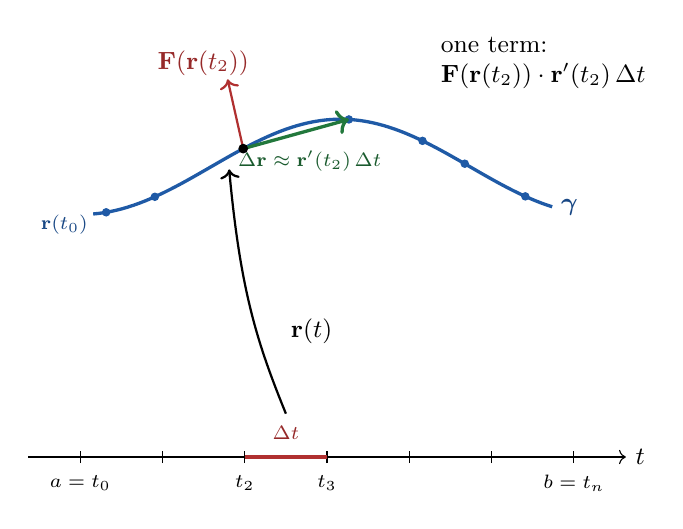
\begin{tikzpicture}[scale=1.1]
% ===== bottom: parameter interval [a,b] with partition =====
\begin{scope}[shift={(0,-2.6)}]
\draw[->] (-0.3,0) -- (6.6,0) node[right, font=\small] {$t$};
\draw[thick] (0.3,0) -- (6.0,0);
\foreach \i in {0,...,6}
  \draw ({0.3+\i*0.95},-0.07) -- ({0.3+\i*0.95},0.07);
\node[below, font=\scriptsize] at (0.3,-0.1) {$a=t_0$};
\node[below, font=\scriptsize] at (2.2,-0.1) {$t_2$};
\node[below, font=\scriptsize] at (3.15,-0.1) {$t_3$};
\node[below, font=\scriptsize] at (6.0,-0.1) {$b=t_n$};
\draw[very thick, figR] (2.2,0) -- (3.15,0);
\node[figR!85!black, font=\scriptsize] at (2.675,0.28) {$\Delta t$};
\end{scope}
% ===== mapping arrow from highlighted subinterval up to the curve =====
\draw[->, thick] (2.675,-2.1) .. controls (2.35,-1.3) and (2.15,-0.7) .. (2.02,0.72);
\node[font=\small, anchor=west] at (2.62,-1.15) {$\mathbf{r}(t)$};
% ===== top: the curve y = 0.75+0.55 sin(1.05x-1.9) =====
\draw[very thick, figB, domain=0.45:5.75, samples=80] plot (\x, {0.75+0.55*sin(deg(1.05*\x-1.9))});
\node[figB!80!black, font=\small] at (5.95,0.28) {$\boldsymbol{\gamma}$};
% image points r(t_j), computed exactly on the curve (uneven spacing = varying speed)
\foreach \px/\py in {0.6/0.225, 1.162/0.404, 2.182/0.96, 3.402/1.297, 4.252/1.05, 4.74/0.786, 5.439/0.409}
  \filldraw[figB] (\px,\py) circle (1.2pt);
\node[font=\scriptsize, figB!80!black, anchor=east] at (0.5,0.08) {$\mathbf{r}(t_0)$};
% chord Delta r from r(t2) to r(t3)
\coordinate (P2) at (2.182,0.96);
\coordinate (P3) at (3.402,1.297);
\draw[->, very thick, figG] (P2) -- (P3);
\node[figG!75!black, font=\scriptsize] at (2.95,0.82) {$\Delta\mathbf{r} \approx \mathbf{r}'(t_2)\,\Delta t$};
% field vector at P2
\draw[->, thick, figR] (P2) -- ++(-0.18,0.80);
\node[figR!85!black, font=\small] at (1.72,1.95) {$\mathbf{F}(\mathbf{r}(t_2))$};
\filldraw (P2) circle (1.4pt);
% term label
\node[font=\small, align=left, anchor=west] at (4.35,1.95) {one term:\\ $\mathbf{F}(\mathbf{r}(t_2)) \cdot \mathbf{r}'(t_2)\,\Delta t$};
\end{tikzpicture}%
\figcap{The line integral is computed through its parametrization: partition \textnormal{time} $[a,b]$ into equal steps $\Delta t$; the map $\mathbf{r}$ pushes the ticks forward to points $\mathbf{r}(t_j)$ on the curve, spaced \textnormal{unevenly} --- wide where the speed $|\mathbf{r}'|$ is large, tight where it is small. Each time step contributes the displacement $\Delta\mathbf{r} \approx \mathbf{r}'(t_j)\Delta t$ and the work term $\mathbf{F}\cdot\Delta\mathbf{r}$. Summing and refining: $\int_{\boldsymbol{\gamma}}\mathbf{F}\cdot d\mathbf{r} = \int_a^b \mathbf{F}(\mathbf{r}(t))\cdot\mathbf{r}'(t)\,dt$ --- an ordinary one-variable integral. The speed factor is automatic: $d\mathbf{r} = \mathbf{r}'(t)\,dt$ is the 1D case of the Jacobian story (\S15).}
\end{center}

Let $\gamma$ be a smooth curve in $\R^2$ parametrized by $x = x(t)$, $y = y(t)$ for $t \in [a, b]$.

\subsection{The Scalar Line Integral (Type I)}

\begin{definition}[Scalar Line Integral]
Let $f: \R^2 \to \R$ be continuous and let $\gamma$ be a piecewise smooth curve. The \textbf{scalar line integral} of $f$ along $\gamma$ is:
\[
\int_\gamma f \, ds = \int_a^b f(x(t), y(t)) \sqrt{x'(t)^2 + y'(t)^2} \, dt.
\]
\end{definition}

\textbf{Derivation.} Partition $[a, b]$ into $a = t_0 < t_1 < \cdots < t_N = b$. The $i$-th piece of $\gamma$ has arc length approximately:
\[
\sqrt{(x(t_i) - x(t_{i-1}))^2 + (y(t_i) - y(t_{i-1}))^2}.
\]

By the Mean Value Theorem, $x(t_i) - x(t_{i-1}) = x'(\xi_i)(t_i - t_{i-1})$ and $y(t_i) - y(t_{i-1}) = y'(\eta_i)(t_i - t_{i-1})$ for some intermediate points. Therefore the arc length of the $i$-th piece is:
\[
\sqrt{x'(\xi_i)^2 + y'(\eta_i)^2} \, (t_i - t_{i-1}).
\]

Weighting each piece by $f(x(t_i), y(t_i))$ and summing:
\[
\sum_{i=1}^N f(x(t_i), y(t_i)) \sqrt{x'(\xi_i)^2 + y'(\eta_i)^2} \, (t_i - t_{i-1}).
\]

Taking $N \to \infty$:
\[
\int_\gamma f \, ds = \int_a^b f(x(t), y(t)) \underbrace{\sqrt{x'(t)^2 + y'(t)^2}}_{ds/dt} \, dt.
\]

\textbf{Physical interpretation:} If $f$ represents a density (mass per unit length), then $\int_\gamma f \, ds$ gives the total mass of a wire shaped like $\gamma$.

\subsection{The Work Line Integral (Type II)}

\begin{definition}[Work Line Integral]
Let $\mathbf{F} = (f(x,y), g(x,y))$ be a continuous vector field. The \textbf{work done by $\mathbf{F}$} along $\gamma$ is:
\[
\int_\gamma f \, dx + g \, dy = \int_a^b \big[ f(x(t), y(t)) \, x'(t) + g(x(t), y(t)) \, y'(t) \big] \, dt.
\]
\end{definition}

\textbf{Derivation.} Along the $i$-th piece, the displacement vector is approximately:
\[
\big( x(t_i) - x(t_{i-1}), \; y(t_i) - y(t_{i-1}) \big).
\]

The force at $(x(t_i), y(t_i))$ is $(f(x(t_i), y(t_i)), \, g(x(t_i), y(t_i)))$. The work done is the inner product of force and displacement:
\begin{align*}
W_i &= f(x(t_i), y(t_i)) \cdot (x(t_i) - x(t_{i-1})) + g(x(t_i), y(t_i)) \cdot (y(t_i) - y(t_{i-1})) \\
&\approx f(x(t_i), y(t_i)) \, x'(t_i)(t_i - t_{i-1}) + g(x(t_i), y(t_i)) \, y'(t_i)(t_i - t_{i-1}).
\end{align*}

Summing and taking the limit:
\[
\sum_{i=1}^N W_i \;\longrightarrow\; \int_a^b \big[ f(x(t), y(t)) \, x'(t) + g(x(t), y(t)) \, y'(t) \big] \, dt.
\]

In differential notation, writing $dx = x'(t) \, dt$ and $dy = y'(t) \, dt$:
\[
\int_\gamma f \, dx + g \, dy = \int_a^b f \, dx(t) + g \, dy(t).
\]

\begin{remark}[Parametrization Independence]
The Type I integral $\int_\gamma f \, ds$ is \textit{independent of orientation}: reversing the direction of traversal does not change the value (since $ds > 0$ always).

The Type II integral $\int_\gamma f \, dx + g \, dy$ \textit{depends on orientation}: reversing the direction of traversal changes the sign (since $dx$ and $dy$ change sign).
\end{remark}

\subsection{Green's Theorem}

For this and the next section, we study the relationship between line integrals and double integrals.

\subsection*{Setup and Orientation Convention}

Let $\gamma$ be a closed curve in $\R^2$ enclosing a bounded domain $D$. The \textbf{positive orientation} of $\gamma$ is defined so that $D$ lies on the left side of $\gamma$ as you traverse it. Equivalently, $\gamma$ is traversed \textbf{counterclockwise}.

\begin{center}
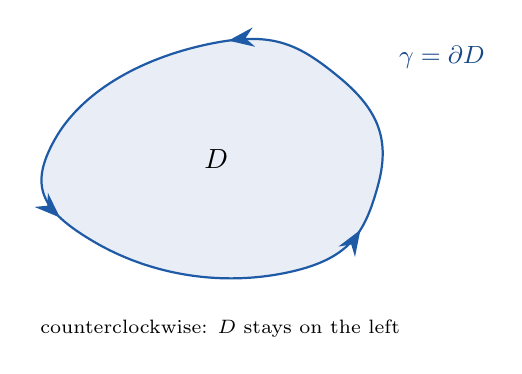
\begin{tikzpicture}[scale=1.0]
% region D
\draw[thick, figB, fill=figB!10,
  postaction={decorate},
  decoration={markings,
    mark=at position 0.10 with {\arrow[figB, scale=1.4]{Stealth}},
    mark=at position 0.42 with {\arrow[figB, scale=1.4]{Stealth}},
    mark=at position 0.74 with {\arrow[figB, scale=1.4]{Stealth}}}]
  plot[smooth cycle, tension=0.85] coordinates {(0,0) (2.4,-0.4) (3.6,0.7) (3.1,2.1) (1.4,2.5) (-0.5,1.3)};
\node at (1.55,1.05) {$D$};
\node[figB!80!black, font=\small, anchor=west] at (3.75,2.35) {$\gamma = \partial D$};
% left-side indicator: small person walking arrow + note
\node[font=\scriptsize, align=center] at (1.6,-1.1) {counterclockwise: $D$ stays on the left};
\end{tikzpicture}%
\figcap{The positive orientation of $\partial D$: traverse counterclockwise, so the region lies on your left. This convention is what makes the signs in Green's theorem come out correctly --- and in \S21 it will reappear as the induced orientation of a boundary.}
\end{center}

Suppose $(f(x,y), g(x,y))$ is a vector field (force field) in the plane. We want to relate $\oint_\gamma f \, dx + g \, dy$ to a double integral over $D$.

\subsection*{Assumption on the Domain}

For convenience, assume $D$ can be represented simultaneously as:
\begin{itemize}
    \item \textbf{Type I} (upper and lower graphs in $x$): $D = \{(x,y) : a \leq x \leq b, \; \phi(x) \leq y \leq \psi(x)\}$
    \item \textbf{Type II} (left and right graphs in $y$): $D = \{(x,y) : c \leq y \leq d, \; \alpha(y) \leq x \leq \beta(y)\}$
\end{itemize}

If $D$ cannot be represented this way (e.g., if $D$ is not convex), we subdivide $D$ into pieces that can, and sum the results. The boundary contributions from internal cuts cancel.

\begin{center}
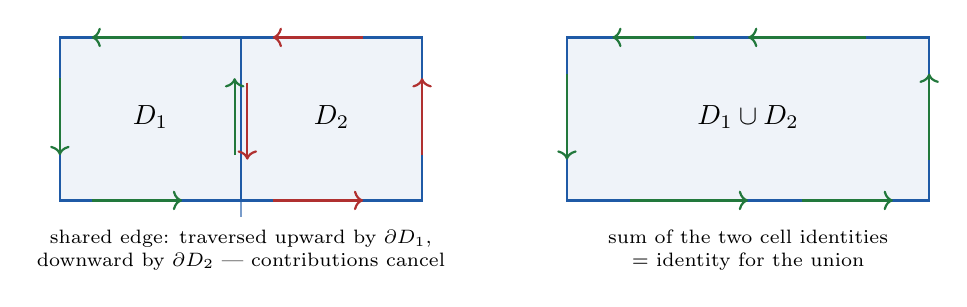
\begin{tikzpicture}[scale=1.15]
% two adjacent cells
\draw[thick, figB, fill=figB!7] (0,0) rectangle (2.0,1.8);
\draw[thick, figB, fill=figB!7] (2.0,0) rectangle (4.0,1.8);
\node at (1.0,0.92) {$D_1$};
\node at (3.0,0.92) {$D_2$};
% ccw orientation arrows on each cell
\draw[->, figG, thick] (0.35,0.0) -- (1.35,0.0);
\draw[->, figG, thick] (1.93,0.5) -- (1.93,1.35);   % D1 right edge: upward
\draw[->, figG, thick] (1.35,1.8) -- (0.35,1.8);
\draw[->, figG, thick] (0,1.35) -- (0,0.5);
\draw[->, figR, thick] (2.35,0.0) -- (3.35,0.0);
\draw[->, figR, thick] (4.0,0.5) -- (4.0,1.35);
\draw[->, figR, thick] (3.35,1.8) -- (2.35,1.8);
\draw[->, figR, thick] (2.07,1.30) -- (2.07,0.45);  % D2 left edge: downward (shifted for visibility)
% highlight shared edge
\node[font=\scriptsize, align=center] at (2.0,-0.55) {shared edge: traversed upward by $\partial D_1$,\\ downward by $\partial D_2$ --- contributions cancel};
\draw[figB!60, thin] (2.0,-0.18) -- (2.0,-0.02);
% right: the merged region with only outer boundary
\begin{scope}[shift={(5.6,0)}]
\draw[thick, figB, fill=figB!7] (0,0) rectangle (4.0,1.8);
\draw[->, figG, thick] (0.7,0.0) -- (2.0,0.0);
\draw[->, figG, thick] (2.6,0.0) -- (3.6,0.0);
\draw[->, figG, thick] (4.0,0.45) -- (4.0,1.4);
\draw[->, figG, thick] (3.3,1.8) -- (2.0,1.8);
\draw[->, figG, thick] (1.4,1.8) -- (0.5,1.8);
\draw[->, figG, thick] (0,1.4) -- (0,0.45);
\node at (2.0,0.92) {$D_1 \cup D_2$};
\node[font=\scriptsize, align=center] at (2.0,-0.55) {sum of the two cell identities\\ $=$ identity for the union};
\end{scope}
\end{tikzpicture}%
\figcap{Why the integral theorems glue: apply the theorem to each cell with its own counterclockwise boundary. The shared internal edge is traversed in opposite directions by the two cells, so its two line-integral contributions cancel exactly, leaving only the outer boundary. This is how the proof extends from rectangles to arbitrary decomposable regions --- and, in \S23, how Stokes' theorem passes from one parameter patch to a whole manifold.}
\end{center}

\subsection*{Derivation: The $\oint f \, dx$ Term}

Consider $\oint_\gamma f \, dx$ using the Type I representation. The boundary $\gamma$ consists of two pieces:
\begin{itemize}
    \item $\gamma_1$: the lower curve $y = \phi(x)$, traversed from $x = a$ to $x = b$ (left to right).
    \item $\gamma_2$: the upper curve $y = \psi(x)$, traversed from $x = b$ to $x = a$ (right to left).
\end{itemize}

(The vertical segments at $x = a$ and $x = b$, if present, contribute zero to $\oint f \, dx$ since $dx = 0$ on them.)

Computing each piece:
\[
\int_{\gamma_1} f \, dx = \int_a^b f(x, \phi(x)) \, dx, \qquad \int_{\gamma_2} f \, dx = \int_b^a f(x, \psi(x)) \, dx = -\int_a^b f(x, \psi(x)) \, dx.
\]

Therefore:
\[
\oint_\gamma f \, dx = \int_a^b \big[ f(x, \phi(x)) - f(x, \psi(x)) \big] \, dx.
\]

By the Fundamental Theorem of Calculus applied to the inner variable $y$:
\[
f(x, \phi(x)) - f(x, \psi(x)) = -\int_{\phi(x)}^{\psi(x)} f_y(x, y) \, dy.
\]

Substituting:
\[
\oint_\gamma f \, dx = -\int_a^b \int_{\phi(x)}^{\psi(x)} f_y(x, y) \, dy \, dx = -\iint_D f_y \, dy \, dx.
\]

\subsection*{Derivation: The $\oint g \, dy$ Term}

Similarly, consider $\oint_\gamma g \, dy$ using the Type II representation. The boundary consists of:
\begin{itemize}
    \item $\gamma_3$: the left curve $x = \alpha(y)$, traversed from $y = d$ to $y = c$ (top to bottom).
    \item $\gamma_4$: the right curve $x = \beta(y)$, traversed from $y = c$ to $y = d$ (bottom to top).
\end{itemize}

Computing:
\[
\int_{\gamma_3} g \, dy = \int_d^c g(\alpha(y), y) \, dy = -\int_c^d g(\alpha(y), y) \, dy, \qquad \int_{\gamma_4} g \, dy = \int_c^d g(\beta(y), y) \, dy.
\]

Therefore:
\[
\oint_\gamma g \, dy = \int_c^d \big[ g(\beta(y), y) - g(\alpha(y), y) \big] \, dy = \int_c^d \int_{\alpha(y)}^{\beta(y)} g_x(x, y) \, dx \, dy = \iint_D g_x \, dx \, dy.
\]

\subsection*{Combining the Two Terms}

Adding the results:

\begin{theorem}[Green's Theorem]
Let $D \subseteq \R^2$ be a bounded domain whose boundary $\gamma = \partial D$ is a piecewise smooth, simple closed curve, oriented counterclockwise. If $f, g$ are $C^1$ on an open set containing $\overline{D}$, then:
\[
\boxed{\oint_\gamma f \, dx + g \, dy = \iint_D \left( \parti{g}{x} - \parti{f}{y} \right) dx \, dy}
\]
\end{theorem}

\begin{remark}[Why the Signs Work Out]
The sign pattern $g_x - f_y$ is not arbitrary. It comes from:
\begin{itemize}
    \item The $\oint f \, dx$ computation gives $-\iint f_y$ (the minus sign comes from the upper curve being traversed right-to-left).
    \item The $\oint g \, dy$ computation gives $+\iint g_x$ (the right curve is traversed bottom-to-top, which is the positive direction).
\end{itemize}
\end{remark}

\begin{remark}[Higher Dimensions]
For the multi-dimensional case, the idea is the same. If a domain in $\R^n$ is bounded by surfaces $x_n = \beta(x_1, \ldots, x_{n-1})$ (upper) and $x_n = \alpha(x_1, \ldots, x_{n-1})$ (lower), we can relate a boundary integral to a volume integral using the Fundamental Theorem of Calculus in the $x_n$ direction. This leads to the \textbf{generalized Stokes' theorem}.
\end{remark}

\subsection{Normal Vectors and Orientation}

Let $\gamma: (x(t), y(t))$, $t \in [a, b]$ be a smooth curve bounding a domain $D$.

\begin{definition}[Tangent and Normal Vectors]
The \textbf{tangent vector} to $\gamma$ at parameter $t$ is:
\[
\mathbf{T}(t) = (x'(t), \, y'(t)).
\]

To obtain a \textbf{normal vector}, we rotate $\mathbf{T}$ by $\pm \frac{\pi}{2}$:
\begin{itemize}
    \item \textbf{Inner normal} (pointing into $D$): rotate $\mathbf{T}$ by $+\frac{\pi}{2}$ counterclockwise: $\mathbf{n}_{\text{in}} = (-y'(t), \, x'(t))$.
    \item \textbf{Outer normal} (pointing out of $D$): rotate $\mathbf{T}$ by $-\frac{\pi}{2}$ clockwise: $\mathbf{n}_{\text{out}} = (y'(t), \, -x'(t))$.
\end{itemize}
\end{definition}

\textbf{Convention:} With $\gamma$ oriented counterclockwise (so $D$ is on our left), the outer normal points to the right of the direction of travel.

\textbf{Verification:} A circle of radius $r$ parametrized as $(r\cos\theta, r\sin\theta)$ has tangent vector $(-r\sin\theta, r\cos\theta)$. The outer normal is:
\[
\mathbf{n}_{\text{out}} = (r\cos\theta, r\sin\theta) \cdot \frac{1}{r} = (\cos\theta, \sin\theta),
\]
which indeed points radially outward. Equivalently, the rotation $(x, y) \mapsto (y, -x)$ applied to the tangent gives the outer normal.

\subsection{The Divergence Theorem (2D)}

We now derive the 2D Divergence Theorem by rewriting Green's theorem in terms of the outward normal.

\subsection*{Rewriting the Line Integral as a Flux Integral}

Parametrize $\gamma$ with $(x(t), y(t))$. The Type II line integral is:
\[
\oint_\gamma f \, dx + g \, dy = \int_a^b \big[ f \, x' + g \, y' \big] \, dt = \int_a^b (f, g) \cdot (x', y') \, dt.
\]

The \textbf{unit outward normal} is $\hat{n} = \dfrac{(y', -x')}{\sqrt{x'^2 + y'^2}}$. A key algebraic observation:
\[
f \, x' + g \, y' = (g, -f) \cdot (y', -x').
\]

(Just expand the right side: $g \, y' + (-f)(-x') = g \, y' + f \, x'$.) Therefore:
\[
\oint_\gamma f \, dx + g \, dy = \int_a^b (g, -f) \cdot (y', -x') \, dt = \int_a^b (g, -f) \cdot \hat{n} \, \sqrt{x'^2 + y'^2} \, dt = \oint_\gamma (g, -f) \cdot \hat{n} \, ds.
\]

This rewrites a work integral as a \textbf{flux integral} of the rotated field $(g, -f)$.

\subsection*{Deriving the Divergence Theorem}

By Green's theorem:
\[
\oint_\gamma (g, -f) \cdot \hat{n} \, ds = \oint_\gamma f \, dx + g \, dy = \iint_D (g_x - f_y) \, dx \, dy.
\]

But $g_x - f_y = g_x + (-f)_y = \nabla \cdot (g, -f)$. So:
\[
\oint_\gamma (g, -f) \cdot \hat{n} \, ds = \iint_D \nabla \cdot (g, -f) \, dx \, dy.
\]

Now rename: let $\mathbf{u} = (u_1, u_2)$ be any $C^1$ vector field. Set $g = u_1$ and $f = -u_2$, so $(g, -f) = (u_1, u_2) = \mathbf{u}$:

\begin{theorem}[Divergence Theorem in $\R^2$]
Let $D \subseteq \R^2$ be a bounded domain with piecewise smooth boundary $\gamma = \partial D$, oriented counterclockwise. If $\mathbf{u} = (u_1, u_2)$ is $C^1$ on an open set containing $\overline{D}$, then:
\[
\boxed{\oint_\gamma \mathbf{u} \cdot \hat{n} \, ds = \iint_D \nabla \cdot \mathbf{u} \, dx \, dy}
\]
where $\nabla \cdot \mathbf{u} = \parti{u_1}{x} + \parti{u_2}{y}$ is the \textbf{divergence} of $\mathbf{u}$, and $\hat{n}$ is the outward unit normal to $\gamma$.
\end{theorem}

\begin{definition}[Divergence]
The \textbf{divergence} of a vector field $\mathbf{u} = (u_1, u_2)$ is the scalar field:
\[
\nabla \cdot \mathbf{u} = \parti{u_1}{x} + \parti{u_2}{y}.
\]

\textbf{Physical interpretation:} $\nabla \cdot \mathbf{u} > 0$ at a point means the field acts as a \textbf{source} (net outflow); $\nabla \cdot \mathbf{u} < 0$ means it acts as a \textbf{sink} (net inflow).
\end{definition}

\begin{example}[Divergence Computations]
\textbf{1.} $\mathbf{u}(x,y) = (x, y)$. Then $\nabla \cdot \mathbf{u} = \partial_x(x) + \partial_y(y) = 1 + 1 = 2$.

Every point is a source with constant strength. This field ``expands'' uniformly.

\textbf{2.} $\mathbf{u}(x,y) = \left(\dfrac{x}{r}, \dfrac{y}{r}\right)$ where $r = \sqrt{x^2 + y^2}$.

\[
\parti{}{x}\left( \frac{x}{r} \right) = \frac{r - x \cdot (x/r)}{r^2} = \frac{r^2 - x^2}{r^3} = \frac{y^2}{r^3}.
\]

Similarly, $\parti{}{y}\left( \dfrac{y}{r} \right) = \dfrac{x^2}{r^3}$. Therefore:
\[
\nabla \cdot \mathbf{u} = \frac{y^2}{r^3} + \frac{x^2}{r^3} = \frac{x^2 + y^2}{r^3} = \frac{r^2}{r^3} = \frac{1}{r}.
\]

The source strength decreases with distance from the origin.
\end{example}

\subsection{Green's Theorem as 2D Stokes' Theorem}

We can also reinterpret Green's theorem using the \textbf{curl}.

\begin{definition}[Curl]
For a vector field $\mathbf{u} = (u_1, u_2, u_3)$ in $\R^3$, the \textbf{curl} is:
\[
\nabla \times \mathbf{u} = \begin{vmatrix} \hat{\imath} & \hat{\jmath} & \hat{k} \\ \partial_x & \partial_y & \partial_z \\ u_1 & u_2 & u_3 \end{vmatrix} = \left( \parti{u_3}{y} - \parti{u_2}{z}, \;\; \parti{u_1}{z} - \parti{u_3}{x}, \;\; \parti{u_2}{x} - \parti{u_1}{y} \right).
\]

(This determinant is a notational mnemonic, not a literal determinant.)
\end{definition}

\textbf{Reduction to 2D.} For a planar vector field $\mathbf{u} = (u_1(x,y), \, u_2(x,y), \, 0)$ (with $u_3 = 0$ and no $z$-dependence):
\[
\nabla \times \mathbf{u} = \left( 0, \; 0, \; \parti{u_2}{x} - \parti{u_1}{y} \right).
\]

The only nonzero component is the $\hat{k}$-component: $(\nabla \times \mathbf{u})_3 = \parti{u_2}{x} - \parti{u_1}{y}$.

This is exactly the integrand in Green's theorem! With $\mathbf{u} = (f, g)$:

\begin{theorem}[Green's Theorem as 2D Stokes' Theorem]
\[
\oint_\gamma \mathbf{u} \cdot d\mathbf{x} = \iint_D (\nabla \times \mathbf{u}) \cdot \hat{k} \, dx \, dy
\]
where $\mathbf{u} = (f, g)$, $d\mathbf{x} = (dx, dy)$, and $(\nabla \times \mathbf{u}) \cdot \hat{k} = g_x - f_y$.
\end{theorem}

\begin{remark}[Two Faces of Green's Theorem]
Green's theorem has two equivalent vector formulations:

\begin{center}
\renewcommand{\arraystretch}{1.5}
\begin{tabular}{|l|c|c|}
\hline
\textbf{Form} & \textbf{Line integral} & \textbf{Area integral} \\
\hline
Circulation (Stokes) & $\oint_\gamma \mathbf{u} \cdot d\mathbf{x}$ & $\iint_D (\nabla \times \mathbf{u}) \cdot \hat{k} \, dA$ \\
\hline
Flux (Divergence) & $\oint_\gamma \mathbf{u} \cdot \hat{n} \, ds$ & $\iint_D \nabla \cdot \mathbf{u} \, dA$ \\
\hline
\end{tabular}
\end{center}

The \textbf{Stokes form} relates the \textit{circulation} of $\mathbf{u}$ around $\gamma$ (tangential component) to the total curl (``rotation'') inside $D$.

The \textbf{Divergence form} relates the \textit{flux} of $\mathbf{u}$ through $\gamma$ (normal component) to the total divergence (``expansion'') inside $D$.

Both generalize to higher dimensions: Stokes' theorem on surfaces in $\R^3$, and the Divergence Theorem on volumes in $\R^3$.
\end{remark}

\section{The Divergence Theorem in Higher Dimensions and Green's Identities}

In the previous section we derived Green's theorem (2D) and its two vector reformulations: the 2D Stokes form (circulation = integral of curl) and the 2D Divergence form (flux = integral of divergence). We now extend the Divergence Theorem to $\R^n$ and derive the classical \textbf{Green's identities}, which are the key tools for studying the Laplacian.

\subsection{The Divergence Theorem in $\R^n$}

\begin{definition}[Divergence in $\R^n$]
For a $C^1$ vector field $\mathbf{u} = (u_1, u_2, \ldots, u_n): D \to \R^n$, the \textbf{divergence} is the scalar field:
\[
\nabla \cdot \mathbf{u} = \sum_{i=1}^n \parti{u_i}{x_i} = \parti{u_1}{x_1} + \parti{u_2}{x_2} + \cdots + \parti{u_n}{x_n}.
\]
\end{definition}

\begin{theorem}[Divergence Theorem in $\R^n$]
\label{thm:div-Rn}
Let $D \subseteq \R^n$ be a bounded domain with piecewise smooth boundary $\partial D$. If $\mathbf{u} = (u_1, \ldots, u_n)$ is $C^1$ on an open set containing $\overline{D}$, then:
\[
\boxed{\int_{\partial D} \mathbf{u} \cdot \hat{n} \, dS = \int_D \nabla \cdot \mathbf{u} \, dV}
\]
where $\hat{n}$ is the outward unit normal to $\partial D$, $dS$ is the surface area element on $\partial D$, and $dV = dx_1 \cdots dx_n$.
\end{theorem}

\begin{proof}
By linearity, it suffices to prove the \textbf{component identity}:
\[
\int_{\partial D} u_k \, n_k \, dS = \int_D \parti{u_k}{x_k} \, dV \qquad \text{for each } k = 1, \ldots, n,
\]
since summing over $k$ gives:
\[
\sum_{k=1}^n \int_{\partial D} u_k \, n_k \, dS = \int_{\partial D} \left( \sum_{k=1}^n u_k \, n_k \right) dS = \int_{\partial D} \mathbf{u} \cdot \hat{n} \, dS
\]
and
\[
\sum_{k=1}^n \int_D \parti{u_k}{x_k} \, dV = \int_D \nabla \cdot \mathbf{u} \, dV.
\]

\textbf{Step 1: Set up.} Fix $k$. For simplicity of notation, we prove the case $k = n$ (the last coordinate); the argument for other $k$ is identical.

Denote the ``horizontal'' variables by $\mathbf{x}' = (x_1, \ldots, x_{n-1})$ and the ``vertical'' variable by $x_n$. Assume $D$ can be written as:
\[
D = \{(\mathbf{x}', x_n) : \mathbf{x}' \in D', \;\; \alpha(\mathbf{x}') \leq x_n \leq \beta(\mathbf{x}')\}
\]
where $D' \subseteq \R^{n-1}$ is the projection of $D$ onto the first $n-1$ coordinates, and $\alpha, \beta: D' \to \R$ are $C^1$ functions describing the ``lower'' and ``upper'' boundary surfaces.

(If $D$ cannot be globally represented this way, we subdivide $D$ into finitely many pieces for which the representation holds. The boundary integrals on the internal cuts cancel in pairs since the outward normals on opposite sides of a cut point in opposite directions.)

\textbf{Step 2: Evaluate the volume integral using FTC.}

By Fubini's theorem, we can write the volume integral as an iterated integral:
\[
\int_D \parti{u_n}{x_n} \, dV = \int_{D'} \left( \int_{\alpha(\mathbf{x}')}^{\beta(\mathbf{x}')} \parti{u_n}{x_n}(\mathbf{x}', x_n) \, dx_n \right) d\mathbf{x}'.
\]

By the Fundamental Theorem of Calculus applied to the inner integral:
\[
\int_{\alpha(\mathbf{x}')}^{\beta(\mathbf{x}')} \parti{u_n}{x_n} \, dx_n = u_n(\mathbf{x}', \beta(\mathbf{x}')) - u_n(\mathbf{x}', \alpha(\mathbf{x}')).
\]

Therefore:
\[
\int_D \parti{u_n}{x_n} \, dV = \int_{D'} \big[ u_n(\mathbf{x}', \beta(\mathbf{x}')) - u_n(\mathbf{x}', \alpha(\mathbf{x}')) \big] \, d\mathbf{x}'. \tag{$\dagger$}
\]

\textbf{Step 3: Evaluate the boundary integral.}

The boundary $\partial D$ consists of three parts:
\begin{itemize}
    \item $S_{\text{top}}$: the upper surface $x_n = \beta(\mathbf{x}')$, parametrized by $\mathbf{x}' \in D'$.
    \item $S_{\text{bot}}$: the lower surface $x_n = \alpha(\mathbf{x}')$, parametrized by $\mathbf{x}' \in D'$.
    \item $S_{\text{side}}$: the lateral boundary (if any), on which $\hat{n}$ is perpendicular to $\hat{e}_n$, so $n_n = 0$.
\end{itemize}

Since $n_n = 0$ on $S_{\text{side}}$, the lateral boundary contributes nothing to $\int_{\partial D} u_n \, n_n \, dS$.

\textit{Upper surface $S_{\text{top}}$:} The surface $x_n = \beta(\mathbf{x}')$ can be written as $F(\mathbf{x}', x_n) = x_n - \beta(\mathbf{x}') = 0$. The outward normal (pointing upward, out of $D$) is:
\[
\hat{n}_{\text{top}} = \frac{\nabla F}{|\nabla F|} = \frac{(-\partial_1 \beta, \ldots, -\partial_{n-1} \beta, 1)}{\sqrt{1 + |\nabla' \beta|^2}},
\]
where $\nabla' \beta = (\partial_1 \beta, \ldots, \partial_{n-1} \beta)$. The surface element is $dS = \sqrt{1 + |\nabla' \beta|^2} \, d\mathbf{x}'$.

Therefore the $n$-th component of $\hat{n}$ times $dS$ is:
\[
n_n \, dS = \frac{1}{\sqrt{1 + |\nabla' \beta|^2}} \cdot \sqrt{1 + |\nabla' \beta|^2} \, d\mathbf{x}' = d\mathbf{x}'.
\]

The contribution from the upper surface is:
\[
\int_{S_{\text{top}}} u_n \, n_n \, dS = \int_{D'} u_n(\mathbf{x}', \beta(\mathbf{x}')) \, d\mathbf{x}'. \tag{$\dagger\dagger_1$}
\]

\textit{Lower surface $S_{\text{bot}}$:} The outward normal now points \textit{downward} (out of $D$), so:
\[
\hat{n}_{\text{bot}} = \frac{(\partial_1 \alpha, \ldots, \partial_{n-1} \alpha, -1)}{\sqrt{1 + |\nabla' \alpha|^2}}.
\]

The $n$-th component gives $n_n \, dS = -d\mathbf{x}'$. Therefore:
\[
\int_{S_{\text{bot}}} u_n \, n_n \, dS = -\int_{D'} u_n(\mathbf{x}', \alpha(\mathbf{x}')) \, d\mathbf{x}'. \tag{$\dagger\dagger_2$}
\]

\textbf{Step 4: Compare.}

Combining $(\dagger\dagger_1)$ and $(\dagger\dagger_2)$:
\[
\int_{\partial D} u_n \, n_n \, dS = \int_{D'} u_n(\mathbf{x}', \beta(\mathbf{x}')) \, d\mathbf{x}' - \int_{D'} u_n(\mathbf{x}', \alpha(\mathbf{x}')) \, d\mathbf{x}' = \int_{D'} \big[ u_n(\mathbf{x}', \beta) - u_n(\mathbf{x}', \alpha) \big] \, d\mathbf{x}'.
\]

This is identical to $(\dagger)$. Therefore:
\[
\int_{\partial D} u_n \, n_n \, dS = \int_D \parti{u_n}{x_n} \, dV.
\]

Repeating the argument for each $k = 1, \ldots, n$ and summing yields the Divergence Theorem.
\end{proof}

\subsection{Green's Identities}

The power of the Divergence Theorem lies in choosing $\mathbf{u}$ strategically. Green's identities arise from specific choices involving scalar functions and the Laplacian.

\begin{definition}[Gradient and Laplacian]
For a $C^2$ function $v: D \to \R$:
\begin{itemize}
    \item The \textbf{gradient} is $\nabla v = \left(\parti{v}{x_1}, \ldots, \parti{v}{x_n}\right)$.
    \item The \textbf{Laplacian} is $\Delta v = \nabla \cdot (\nabla v) = \displaystyle\sum_{i=1}^n \frac{\partial^2 v}{\partial x_i^2}$.
    \item The \textbf{normal derivative} on $\partial D$ is $\dfrac{\partial v}{\partial n} = \nabla v \cdot \hat{n} = \displaystyle\sum_{i=1}^n \parti{v}{x_i} \, n_i$.
\end{itemize}
\end{definition}

\subsection*{Green's First Identity}

\begin{theorem}[Green's First Identity]
\label{thm:green1}
Let $D \subseteq \R^n$ be a bounded domain with piecewise smooth boundary. If $u \in C^1(\overline{D})$ and $v \in C^2(\overline{D})$, then:
\[
\boxed{\int_D \big( \nabla u \cdot \nabla v + u \, \Delta v \big) \, dV = \int_{\partial D} u \, \frac{\partial v}{\partial n} \, dS}
\]

Equivalently (rearranging):
\[
\int_D u \, \Delta v \, dV = \int_{\partial D} u \, \frac{\partial v}{\partial n} \, dS - \int_D \nabla u \cdot \nabla v \, dV.
\]

This is the \textbf{higher-dimensional integration by parts}: the ``derivative'' ($\Delta$) is transferred from $v$ to $u$ (as $\nabla u$), at the cost of a boundary term.
\end{theorem}

\begin{proof}
Apply the Divergence Theorem (Theorem~\ref{thm:div-Rn}) with the vector field $\mathbf{w} = u \, \nabla v$.

\textbf{Step 1: Compute the divergence of $\mathbf{w}$.}

The $i$-th component of $\mathbf{w}$ is $w_i = u \, \parti{v}{x_i}$. By the product rule:
\[
\parti{w_i}{x_i} = \parti{u}{x_i} \cdot \parti{v}{x_i} + u \cdot \frac{\partial^2 v}{\partial x_i^2}.
\]

Summing over $i$:
\[
\nabla \cdot \mathbf{w} = \sum_{i=1}^n \parti{w_i}{x_i} = \sum_{i=1}^n \parti{u}{x_i} \parti{v}{x_i} + u \sum_{i=1}^n \frac{\partial^2 v}{\partial x_i^2} = \nabla u \cdot \nabla v + u \, \Delta v.
\]

\textbf{Step 2: Compute the boundary term.}

\[
\mathbf{w} \cdot \hat{n} = (u \, \nabla v) \cdot \hat{n} = u \, (\nabla v \cdot \hat{n}) = u \, \frac{\partial v}{\partial n}.
\]

\textbf{Step 3: Apply the Divergence Theorem.}

\[
\int_{\partial D} u \, \frac{\partial v}{\partial n} \, dS = \int_{\partial D} \mathbf{w} \cdot \hat{n} \, dS = \int_D \nabla \cdot \mathbf{w} \, dV = \int_D \big( \nabla u \cdot \nabla v + u \, \Delta v \big) \, dV. \qedhere
\]
\end{proof}

\begin{remark}[Special Case: $u = v$]
Setting $u = v$ in Green's first identity:
\[
\int_D \big( |\nabla v|^2 + v \, \Delta v \big) \, dV = \int_{\partial D} v \, \frac{\partial v}{\partial n} \, dS.
\]

If in addition $v$ is \textbf{harmonic} ($\Delta v = 0$) and $v = 0$ on $\partial D$, then:
\[
\int_D |\nabla v|^2 \, dV = 0 \quad \Longrightarrow \quad \nabla v \equiv 0 \quad \Longrightarrow \quad v \equiv 0 \text{ on } D.
\]

This proves \textbf{uniqueness for the Dirichlet problem}: if $\Delta v = 0$ on $D$ and $v = 0$ on $\partial D$, then $v = 0$. Equivalently, a harmonic function is uniquely determined by its boundary values.
\end{remark}

\subsection*{Green's Second Identity}

\begin{theorem}[Green's Second Identity]
\label{thm:green2}
Let $D \subseteq \R^n$ be a bounded domain with piecewise smooth boundary. If $u, v \in C^2(\overline{D})$, then:
\[
\boxed{\int_D \big( u \, \Delta v - v \, \Delta u \big) \, dV = \int_{\partial D} \left( u \, \frac{\partial v}{\partial n} - v \, \frac{\partial u}{\partial n} \right) dS}
\]
\end{theorem}

\begin{proof}
Apply Green's first identity (Theorem~\ref{thm:green1}) twice, then subtract.

\textbf{Step 1:} Apply with $(u, v)$:
\[
\int_D (\nabla u \cdot \nabla v + u \, \Delta v) \, dV = \int_{\partial D} u \, \frac{\partial v}{\partial n} \, dS. \tag{$\star$}
\]

\textbf{Step 2:} Apply with the roles of $u$ and $v$ swapped:
\[
\int_D (\nabla v \cdot \nabla u + v \, \Delta u) \, dV = \int_{\partial D} v \, \frac{\partial u}{\partial n} \, dS. \tag{$\star\star$}
\]

\textbf{Step 3:} Subtract $(\star\star)$ from $(\star)$. On the left side, $\nabla u \cdot \nabla v = \nabla v \cdot \nabla u$, so these terms cancel:
\[
\int_D (u \, \Delta v - v \, \Delta u) \, dV = \int_{\partial D} \left( u \, \frac{\partial v}{\partial n} - v \, \frac{\partial u}{\partial n} \right) dS. \qedhere
\]
\end{proof}

\begin{remark}[Green's Second Identity as Symmetry]
Green's second identity expresses a kind of \textbf{symmetry of the Laplacian}: the ``interaction'' of $u$ with $\Delta v$ differs from the interaction of $v$ with $\Delta u$ only by a boundary term. This is the $L^2$ analog of integration by parts, and it shows that the Laplacian is a \textbf{self-adjoint operator} (up to boundary terms).

In more advanced treatments, this property is the starting point for Sturm--Liouville theory, spectral theory, and the theory of distributions.
\end{remark}

\subsection{Applications of Green's Identities}

\begin{example}[Uniqueness for the Dirichlet Problem]
\textbf{Claim:} If $\Delta u_1 = \Delta u_2$ on $D$ and $u_1 = u_2$ on $\partial D$, then $u_1 = u_2$ on $D$.

\textit{Proof.} Let $w = u_1 - u_2$. Then $\Delta w = 0$ on $D$ and $w = 0$ on $\partial D$. Apply Green's first identity with $u = v = w$:
\[
\int_D |\nabla w|^2 \, dV + \underbrace{\int_D w \, \Delta w \, dV}_{= 0} = \underbrace{\int_{\partial D} w \, \frac{\partial w}{\partial n} \, dS}_{= 0}.
\]

Therefore $\int_D |\nabla w|^2 \, dV = 0$. Since $|\nabla w|^2 \geq 0$ and is continuous, this implies $\nabla w = 0$ on $D$, so $w$ is constant. Since $w = 0$ on $\partial D$, we conclude $w \equiv 0$.
\end{example}

\begin{example}[Uniqueness for the Neumann Problem]
\textbf{Claim:} If $\Delta u_1 = \Delta u_2$ on $D$ and $\dfrac{\partial u_1}{\partial n} = \dfrac{\partial u_2}{\partial n}$ on $\partial D$, then $u_1 - u_2$ is constant on $D$.

\textit{Proof.} Let $w = u_1 - u_2$. Then $\Delta w = 0$ and $\dfrac{\partial w}{\partial n} = 0$ on $\partial D$. Green's first identity with $u = v = w$:
\[
\int_D |\nabla w|^2 \, dV = \int_{\partial D} w \, \underbrace{\frac{\partial w}{\partial n}}_{= 0} \, dS = 0.
\]

So $\nabla w = 0$, hence $w$ is constant. (Note: unlike Dirichlet, we cannot determine the constant --- this is why Neumann solutions are unique only up to a constant.)
\end{example}

\begin{example}[Mean Value Property of Harmonic Functions (Sketch)]
Green's identities can be used to prove the \textbf{mean value property}: if $\Delta u = 0$ on a ball $B_r(x_0) \subseteq \R^n$, then:
\[
u(x_0) = \frac{1}{|\partial B_r|} \int_{\partial B_r(x_0)} u \, dS,
\]
i.e., the value of a harmonic function at any point equals its average over any sphere centered at that point. The proof uses Green's second identity with $v$ chosen as the \textbf{fundamental solution} of the Laplacian ($v = |x - x_0|^{2-n}$ for $n \geq 3$, or $v = \log |x - x_0|$ for $n = 2$).
\end{example}

\begin{remark}[Summary: The Hierarchy of Integral Theorems]
All the integral theorems in this course are instances of a single pattern:

\begin{center}
\renewcommand{\arraystretch}{1.5}
\begin{tabular}{|l|c|}
\hline
\textbf{Theorem} & \textbf{Pattern} \\
\hline
Fundamental Theorem of Calculus & $\int_a^b F'(x) \, dx = F(b) - F(a)$ \\
\hline
Green's Theorem (2D) & $\iint_D (g_x - f_y) \, dA = \oint_{\partial D} f \, dx + g \, dy$ \\
\hline
Divergence Theorem ($\R^n$) & $\int_D \nabla \cdot \mathbf{u} \, dV = \int_{\partial D} \mathbf{u} \cdot \hat{n} \, dS$ \\
\hline
Stokes' Theorem ($\R^3$) & $\iint_S (\nabla \times \mathbf{F}) \cdot d\mathbf{S} = \oint_{\partial S} \mathbf{F} \cdot d\mathbf{r}$ \\
\hline
\end{tabular}
\end{center}

In each case: \textit{integral of a derivative over a region = integral of the function over the boundary}.

In the language of differential forms (to be covered if time permits), all of these are special cases of the \textbf{generalized Stokes' theorem}: $\displaystyle\int_{\partial \Omega} \omega = \int_\Omega d\omega$.
\end{remark}

\subsection{Physical Application: Conservation of Mass and Laplace's Equation}

\subsection*{Flux and the Continuity Equation}

Consider a fluid with density $\rho(x, y, t)$ and velocity field $\mathbf{u}(x, y, t)$. Let $D$ be a fixed region in the plane with boundary $\gamma$.

\textbf{Rate of change of outflow of volume} across $\gamma$: if the flow speed is $u$ in a pipe of cross-section $S$, the volume displaced in time $T$ is $uTS$, so the volume flux per unit time is $uS$. For a general boundary:
\[
\text{rate of outflow of volume} = \oint_\gamma \mathbf{u} \cdot \hat{n} \, ds.
\]

\textbf{Rate of change of outflow of mass} across $\gamma$: weight by density:
\[
\text{rate of outflow of mass} = \oint_\gamma \rho \, \mathbf{u} \cdot \hat{n} \, ds.
\]

\textbf{Mass in $D$:}
\[
\text{mass in } D = \iint_D \rho \, dx \, dy.
\]

\textbf{Rate of change of mass in $D$:}
\[
\frac{d}{dt} \iint_D \rho \, dx \, dy = \iint_D \rho_t \, dx \, dy.
\]

If there are no sources or sinks ($\rho > 0$, mass is neither created nor destroyed), then conservation of mass says:
\[
\underbrace{\frac{d}{dt} \iint_D \rho \, dx \, dy}_{\text{rate of change of mass in } D} + \underbrace{\oint_\gamma \rho \, \mathbf{u} \cdot \hat{n} \, ds}_{\text{rate of outflow of mass}} = 0. \tag{$\textcircled{1} + \textcircled{2} = 0$}
\]

Now apply the Divergence Theorem to $\textcircled{2}$:
\[
\oint_\gamma \rho \, \mathbf{u} \cdot \hat{n} \, ds = \oint_\gamma (\rho \mathbf{u}) \cdot \hat{n} \, ds = \iint_D \nabla \cdot (\rho \mathbf{u}) \, dx \, dy.
\]

Substituting both terms:
\[
\iint_D \big( \rho_t + \nabla \cdot (\rho \mathbf{u}) \big) \, dx \, dy = 0 \qquad \text{for \textbf{any} domain } D.
\]

\textbf{Key argument:} If $\iint_D f \, dx \, dy = 0$ for every domain $D$ and $f$ is continuous, then $f \equiv 0$. (If $f(a,b) > 0$, then by continuity $f \geq f(a,b)/2 > 0$ on some ball $B_\delta(a,b) \subseteq D$, giving a positive integral --- contradiction.)

Therefore, the integrand vanishes pointwise:

\begin{theorem}[Continuity Equation / Conservation of Mass]
\[
\boxed{\rho_t + \nabla \cdot (\rho \mathbf{u}) = 0}
\]
\end{theorem}

This is the \textbf{continuity equation}: the local form of conservation of mass.

\subsection*{Incompressible Flow}

Assume the fluid has constant density $\rho \equiv 1$ (incompressible). Then $\rho_t = 0$ and $\nabla \cdot (\rho \mathbf{u}) = \nabla \cdot \mathbf{u}$, so the continuity equation reduces to:
\[
\nabla \cdot \mathbf{u} = 0 \qquad \text{(divergence-free / incompressible)}.
\]

\subsection*{Irrotational Flow}

An additional physical condition: the flow is \textbf{irrotational} (no rotation), meaning:
\[
\nabla \times \mathbf{u} = 0 \qquad \text{(curl-free / irrotational)}.
\]

Writing $\mathbf{u} = (u, v)$, the two conditions become the system:
\[
\begin{cases} u_x + v_y = 0 & (\text{divergence-free}) \\ v_x - u_y = 0 & (\text{curl-free}) \end{cases}
\]

\subsection*{From Potential Functions to Laplace's Equation}

\textbf{Physical motivation:} If the flow is driven by a potential (e.g., gravity), there exists a \textbf{potential function} $\phi(x,y)$ such that contour lines $\phi(x,y) = c$ are level curves of energy. The gradient $\nabla \phi = (\phi_x, \phi_y)$ points in the direction of increasing energy, and the fluid flows in the \textit{opposite} direction:
\[
\mathbf{u} = (u, v) = -\nabla \phi = (-\phi_x, -\phi_y).
\]

\textbf{Check curl-free:} With $u = -\phi_x$ and $v = -\phi_y$:
\[
v_x - u_y = -\phi_{yx} - (-\phi_{xy}) = -\phi_{yx} + \phi_{xy} = 0
\]
by equality of mixed partials. So the curl-free condition is \textit{automatically satisfied} for any potential function. This is a general fact: $\nabla \times (\nabla \phi) = 0$ always.

\textbf{Apply the divergence-free condition:}
\[
u_x + v_y = -\phi_{xx} - \phi_{yy} = 0 \qquad \Longleftrightarrow \qquad \boxed{\Delta \phi = \phi_{xx} + \phi_{yy} = 0.}
\]

This is \textbf{Laplace's equation}. A function satisfying $\Delta \phi = 0$ is called \textbf{harmonic}.

\begin{remark}[Summary of the Logical Chain]
\[
\text{Conservation of mass} + \text{incompressible} + \text{irrotational} \quad \Longrightarrow \quad \text{Laplace's equation } \Delta \phi = 0.
\]

The problem of finding incompressible irrotational flow reduces to: find a potential function $\phi(x,y)$ satisfying $\Delta \phi = 0$ with appropriate boundary conditions. This is the \textbf{Dirichlet problem}, whose uniqueness we proved using Green's first identity.
\end{remark}

\begin{remark}[Symmetry and Radial Solutions]
Laplace's equation $\phi_{xx} + \phi_{yy} = 0$ has a symmetric structure: the operator $\Delta$ treats $x$ and $y$ on equal footing. This symmetry motivates looking for \textbf{radial solutions}, i.e., solutions depending only on $r = \sqrt{x^2 + y^2}$: $\phi(x,y) = f(r)$.
\end{remark}

\subsection*{Computing $\Delta \phi$ for a Radial Function}

Let $\phi(x,y) = f(r)$ where $r = \sqrt{x^2 + y^2}$. We compute $\phi_{xx}$ and $\phi_{yy}$ via the chain rule.

\textbf{First derivatives of $r$:}
\[
r_x = \frac{x}{r}, \qquad r_y = \frac{y}{r}.
\]

\textbf{Second derivatives of $r$:}
\[
r_{xx} = \parti{}{x}\left(\frac{x}{r}\right) = \frac{r - x \cdot (x/r)}{r^2} = \frac{r^2 - x^2}{r^3}, \qquad r_{yy} = \frac{r^2 - y^2}{r^3}.
\]

\textbf{First derivative of $\phi$:}
\[
\phi_x = f'(r) \cdot r_x = f'(r) \cdot \frac{x}{r}.
\]

\textbf{Second derivative of $\phi$:} Using the product rule on $\phi_x = f'(r) \cdot r_x$:
\begin{align*}
\phi_{xx} &= \parti{}{x}\big(f'(r) \cdot r_x\big) = \big(f'(r)\big)_x \cdot r_x + f'(r) \cdot r_{xx} \\
&= f''(r) \cdot r_x \cdot r_x + f'(r) \cdot r_{xx} \\
&= f''(r) \cdot \frac{x^2}{r^2} + f'(r) \cdot \frac{r^2 - x^2}{r^3}.
\end{align*}

By the same argument (replacing $x$ with $y$):
\[
\phi_{yy} = f''(r) \cdot \frac{y^2}{r^2} + f'(r) \cdot \frac{r^2 - y^2}{r^3}.
\]

\textbf{The Laplacian:}
\begin{align*}
\Delta \phi = \phi_{xx} + \phi_{yy} &= f''(r) \cdot \frac{x^2 + y^2}{r^2} + f'(r) \cdot \frac{2r^2 - x^2 - y^2}{r^3} \\
&= f''(r) \cdot \frac{r^2}{r^2} + f'(r) \cdot \frac{2r^2 - r^2}{r^3} \\
&= f''(r) + \frac{f'(r)}{r}.
\end{align*}

\subsection*{Solving the Radial ODE}

Setting $\Delta \phi = 0$:
\[
f''(r) + \frac{1}{r} f'(r) = 0.
\]

\textbf{Step 1: Reduce order.} Let $g(r) = f'(r)$. Then:
\[
g'(r) + \frac{g(r)}{r} = 0.
\]

\textbf{Step 2: Separate variables.}
\[
\frac{dg}{g} = -\frac{dr}{r}.
\]

\textbf{Step 3: Integrate both sides.}
\[
\ln|g| = -\ln|r| + C_1 \qquad \Longrightarrow \qquad |g| = e^{C_1} \cdot \frac{1}{r} = \frac{C_2}{r}.
\]

So $g(r) = C/r$ for some constant $C$.

\textbf{Verification:} $g'(r) = -C/r^2$, so $g'(r) + g(r)/r = -C/r^2 + C/r^2 = 0$. \checkmark

\textbf{Step 4: Recover $f$.}
\[
f'(r) = g(r) = \frac{C}{r} \qquad \Longrightarrow \qquad f(r) = C \ln r + C'.
\]

Choosing $C' = 0$:

\begin{theorem}[Fundamental Solution of the 2D Laplacian]
The function
\[
\phi(x,y) = C \ln r = C \ln \sqrt{x^2 + y^2}
\]
satisfies Laplace's equation $\Delta \phi = 0$ for all $(x,y) \neq (0,0)$.
\end{theorem}

\begin{remark}[Connection to Other PDEs]
This fundamental solution is the starting point for solving boundary value problems via Green's functions. The same approach --- exploit symmetry to reduce a PDE to an ODE --- applies to other equations:
\begin{itemize}
    \item \textbf{Laplace's equation} $\Delta \phi = 0$: steady-state (time-independent) problems.
    \item \textbf{Heat equation} $\phi_t = \Delta \phi$: diffusion and heat conduction (time-dependent).
    \item \textbf{Wave equation} $\phi_{tt} = c^2 \Delta \phi$: vibrations and wave propagation.
\end{itemize}
\end{remark}

\chapter{Surface Integrals and the Classical Theorems}

\section{Surface Integrals}

\begin{note}[Smoothness Assumptions for This Section]
The results in this section require increasingly strong conditions on the parametrization $\mathbf{X}$, the surface $S$, and the vector field $\mathbf{F}$. Here is the hierarchy, from weakest to strongest:

\begin{enumerate}[itemsep=4pt]
    \item \textbf{Tangent vectors exist:} $\mathbf{X}: D \to \R^3$ is $C^1$ (i.e., all partial derivatives $x_u, x_v, y_u, y_v, z_u, z_v$ exist and are continuous). This ensures the tangent vectors $\mathbf{X}_u, \mathbf{X}_v$ are well-defined and vary continuously.

    \item \textbf{The parametrization describes a surface (regularity):} $\mathbf{X}$ is $C^1$ \textit{and} the Jacobian $D\mathbf{X}$ has rank 2 everywhere, i.e., $\mathbf{X}_u \times \mathbf{X}_v \neq \mathbf{0}$. This ensures a well-defined tangent plane at every point, and in particular ensures $|\mathbf{X}_u \times \mathbf{X}_v| > 0$ so the area element $dS$ is nondegenerate.

    \item \textbf{The parametrization is injective} (on the interior of $D$): distinct parameter values give distinct surface points, so the surface does not self-intersect. Without this, the ``surface area'' might count some regions of $S$ multiple times.

    \item \textbf{Orientability:} A continuous choice of unit normal $\hat{n}$ exists on all of $S$. This is needed for flux integrals (otherwise the sign of $\mathbf{F} \cdot \hat{n}$ is ambiguous). A regular parametrization automatically provides an orientation via $\hat{n} = (\mathbf{X}_u \times \mathbf{X}_v) / |\mathbf{X}_u \times \mathbf{X}_v|$; the question is whether different parametrizations of the same surface give consistent normals. (The M\"obius strip is the classical example of a non-orientable surface.)

    \item \textbf{For the integral theorems} (Divergence, Stokes): the boundary $\partial V$ or $\partial S$ must be \textbf{piecewise smooth} (finitely many smooth pieces joined along curves or edges), and the vector field $\mathbf{F}$ must be $C^1$ on an open set containing $\overline{V}$ (or $\overline{S}$). The piecewise smoothness allows us to decompose into pieces on which the proof works, and the $C^1$ condition on $\mathbf{F}$ ensures the divergence $\nabla \cdot \mathbf{F}$ (or curl $\nabla \times \mathbf{F}$) exists and is continuous.
\end{enumerate}

\textbf{Standing assumption for this section:} Unless stated otherwise, all parametrizations are $C^1$, injective on the interior of $D$, and regular. All surfaces are oriented. All vector fields are $C^1$.
\end{note}

\subsection{Parametrized Surfaces}

\subsection*{What is a Surface?}

A \textbf{surface} $S$ is a subset of $\R^3$ that is locally two-dimensional: near any point, it ``looks like'' a piece of $\R^2$ that has been bent and placed into 3D space. Examples include spheres, cylinders, tori, and graphs $z = h(x,y)$.

\textbf{The problem:} To do calculus on $S$ (integrate functions, compute areas, etc.), we need a way to systematically describe \textit{which points} belong to $S$. We need a coordinate system on $S$.

\subsection*{Parametrization as a Coordinate System}

We already understand curves: a curve in $\R^3$ is a map $t \mapsto \boldsymbol{\gamma}(t) = (x(t), y(t), z(t))$, one parameter tracing out a 1D object. A surface can be thought of as a \textbf{family of curves}: fix one parameter, say $u = u_0$, and let the other vary --- the map $v \mapsto \mathbf{X}(u_0, v)$ traces out a curve on $S$. Now let $u_0$ vary continuously: the curve deforms, sweeping out a 2D region. The surface is the union of all these curves, one for each value of $u$.

So a \textbf{parametrization} labels every point on $S$ by two numbers $(u,v)$: one parameter ($v$) tells you where you are \textit{along} a particular curve, and the other ($u$) tells you \textit{which curve} you are on. Since a point in $\R^3$ is specified by $(x,y,z)$, this is a function:
\[
(u, v) \;\mapsto\; \text{point } \big( x(u,v), \, y(u,v), \, z(u,v) \big) \in S.
\]

We write this as $\mathbf{X}(u,v) = (x(u,v), y(u,v), z(u,v))$. Here:
\begin{itemize}
    \item The domain $D \subseteq \R^2$ is the \textbf{parameter space} --- a flat 2D region. Think of it as a ``blueprint'' for the surface.
    \item For each $(u,v) \in D$, the output $\mathbf{X}(u,v) \in \R^3$ is the \textbf{position} of the corresponding point on $S$. It is a vector only in the sense that points in $\R^3$ are identified with their position vectors from the origin; $\mathbf{X}(u,v)$ tells you \textit{where the point sits} in 3D space.
    \item The surface is the image: $S = \mathbf{X}(D) = \{\mathbf{X}(u,v) : (u,v) \in D\}$.
\end{itemize}

The parametrization $\mathbf{X}: D \to \R^3$ is a ``change of variables from 2D to 3D'': it takes a flat rectangle (or other 2D region) and wraps it into a curved surface in $\R^3$.

\begin{definition}[Parametrized Surface]
A \textbf{parametrized surface} in $\R^3$ is a $C^1$ map $\mathbf{X}: D \to \R^3$, where $D \subseteq \R^2$ is a domain, given by
\[
\mathbf{X}(u, v) = \big( x(u,v), \, y(u,v), \, z(u,v) \big).
\]

The image $S = \mathbf{X}(D) \subseteq \R^3$ is the \textbf{surface}, and $(u,v)$ are its \textbf{parameters} (coordinates on $S$).
\end{definition}

\begin{example}[Sphere]
The unit sphere $S^2 = \{(x,y,z) : x^2 + y^2 + z^2 = R^2\}$ is a set of points in $\R^3$. To parametrize it, we use spherical angles $(\theta, \varphi)$:
\[
\mathbf{X}(\theta, \varphi) = (R\cos\varphi\cos\theta, \; R\cos\varphi\sin\theta, \; R\sin\varphi),
\]
with $\theta \in [0, 2\pi)$ and $\varphi \in (-\pi/2, \pi/2)$.

Here $\mathbf{X}(\theta, \varphi)$ tells you: ``the point on the sphere at longitude $\theta$ and latitude $\varphi$ has Cartesian coordinates $(R\cos\varphi\cos\theta, R\cos\varphi\sin\theta, R\sin\varphi)$.''
\end{example}

\begin{remark}[Dimension Count]
A 1D object (curve) in 1D space cannot curve --- it fills the whole space. A 1D object in 2D space \textit{can} curve. Similarly, a surface is a 2D object that can curve only when it lives in 3D (or higher) space. The parametrization $\mathbf{X}: \R^2 \to \R^3$ maps a flat 2D domain into 3D, and the image can be curved.
\end{remark}

\subsection{Tangent Vectors and Regularity}

Fix a point $(u_0, v_0) \in D$. The two families of curves through this point give two tangent directions:
\begin{itemize}
    \item The \textbf{$u$-curve} $u \mapsto \mathbf{X}(u, v_0)$ (fix $v$, vary $u$) has tangent vector $\mathbf{X}_u$.
    \item The \textbf{$v$-curve} $v \mapsto \mathbf{X}(u_0, v)$ (fix $u$, vary $v$) has tangent vector $\mathbf{X}_v$.
\end{itemize}

These are exactly the tangent vectors to the two families of curves that sweep out the surface.

\begin{definition}[Tangent Vectors]
The \textbf{tangent vectors} to the surface at $(u_0, v_0)$ are:
\[
\mathbf{X}_u = \left( \parti{x}{u}, \, \parti{y}{u}, \, \parti{z}{u} \right), \qquad \mathbf{X}_v = \left( \parti{x}{v}, \, \parti{y}{v}, \, \parti{z}{v} \right).
\]
\end{definition}

\begin{center}
\includegraphics[width=0.92\textwidth]{pyfigs/f7_param_surface.pdf}%
\figcap{The surface integral is computed cell by cell: a grid cell $\Delta u \times \Delta v$ in the parameter domain (red, left) is carried by $\mathbf{X}$ to a curved patch on the surface (red, right). Zoomed to this scale, the patch is approximated by the tangent parallelogram (green) spanned by $\mathbf{X}_u\Delta u$ and $\mathbf{X}_v\Delta v$, with area $|\mathbf{X}_u \times \mathbf{X}_v|\,\Delta u\,\Delta v$. Summing over all cells and refining gives $\iint_S dS = \iint_D |\mathbf{X}_u \times \mathbf{X}_v|\,du\,dv$: the cross product length is the area-scaling factor, playing exactly the role $|J|$ played in \S15 --- and $|\mathbf{r}'|$ in \S16.}
\end{center}

\begin{definition}[Regular Point]
The surface is \textbf{regular} at $(u_0, v_0)$ if $\mathbf{X}_u$ and $\mathbf{X}_v$ are linearly independent at that point, i.e., $\mathbf{X}_u \times \mathbf{X}_v \neq \mathbf{0}$.

A surface is \textbf{regular} if it is regular at every point of $D$.
\end{definition}

\textbf{Geometric meaning:} At a regular point, the $u$-curves and $v$-curves cross transversally, spanning a 2D tangent plane. If $\mathbf{X}_u$ and $\mathbf{X}_v$ are parallel (or one is zero), the two families of curves are tangent to each other --- they fail to sweep out a genuine 2D surface at that point, and the parametrization degenerates.

\begin{remark}[Regularity as a Rank Condition on the Derivative]
The regularity condition is best understood through the differentiability framework of Section 6, applied to $\mathbf{X}: \R^2 \to \R^3$.

\textbf{The derivative of $\mathbf{X}$.} Differentiability of $\mathbf{X}$ at $(u_0, v_0)$ means:
\[
\mathbf{X}(u_0 + h, v_0 + k) = \mathbf{X}(u_0, v_0) + D\mathbf{X} \begin{pmatrix} h \\ k \end{pmatrix} + o\!\left(\sqrt{h^2 + k^2}\right)
\]
where $D\mathbf{X}$ is the $3 \times 2$ Jacobian matrix whose columns are $\mathbf{X}_u$ and $\mathbf{X}_v$:
\[
D\mathbf{X} = \begin{pmatrix} x_u & x_v \\ y_u & y_v \\ z_u & z_v \end{pmatrix}.
\]

The image of $D\mathbf{X}$ --- the set of all vectors $h \mathbf{X}_u + k \mathbf{X}_v$ --- is the \textbf{tangent space}. Its dimension equals $\operatorname{rank}(D\mathbf{X})$:
\begin{itemize}
    \item \textbf{Rank 2} ($\mathbf{X}_u, \mathbf{X}_v$ independent, i.e., regular): the image of $D\mathbf{X}$ is a 2D plane. The linear approximation faithfully represents a 2D surface. This is the good case.
    \item \textbf{Rank 1} ($\mathbf{X}_u, \mathbf{X}_v$ parallel): the image is a line. The derivative compresses two dimensions into one --- the parametrization ``folds'' the $(u,v)$-plane onto a curve at that point.
    \item \textbf{Rank 0} ($\mathbf{X}_u = \mathbf{X}_v = \mathbf{0}$): the image is a point. The derivative gives zero information about the surface.
\end{itemize}

So the surface is differentiable in all three cases (the linear approximation exists), but \textbf{regularity ensures the approximation is full-dimensional} --- that it is actually approximating a \textit{surface} and not a lower-dimensional object.

\textbf{Parallel to earlier results.} This is the same idea as the change of variables theorem and the IFT:
\begin{itemize}
    \item In the \textbf{change of variables} (Section 14), $J \neq 0$ means the $2 \times 2$ Jacobian has rank 2, ensuring the map is locally invertible.
    \item In the \textbf{IFT/Inverse FT} (Sections 11--12), the nonvanishing determinant ensures the derivative has full rank.
    \item Here, $\mathbf{X}_u \times \mathbf{X}_v \neq \mathbf{0}$ means the $3 \times 2$ Jacobian has rank 2, ensuring the parametrization is locally injective (an \textbf{immersion}) --- it does not collapse any direction.
\end{itemize}

This also explains why $\det(G) = |\mathbf{X}_u \times \mathbf{X}_v|^2$ appears in the area formula: it measures how much 2D area the derivative preserves. When $\det(G) = 0$, the derivative crushes some 2D area to zero --- exactly the degenerate case.

\textbf{Irregular point $\neq$ singular surface.} An irregular point can mean two different things:
\begin{itemize}
    \item \textbf{Bad parametrization, smooth surface.} The sphere parametrized by $(\theta, \varphi)$ has $\mathbf{X}_\theta = \mathbf{0}$ at the poles ($\varphi = \pm \pi/2$), because all values of $\theta$ map to the same point. The sphere is perfectly smooth there; the coordinate system degenerates. A different parametrization (e.g., centered at the pole) would be regular.
    \item \textbf{Genuinely singular surface.} The cone $\mathbf{X}(u,v) = (v\cos u, v\sin u, v)$ has $\mathbf{X}_u = \mathbf{0}$ at the tip $v = 0$. No reparametrization can fix this --- the cone tip has no well-defined tangent plane; it is not a smooth 2D surface.
\end{itemize}

Distinguishing these cases requires checking whether the singularity persists under all possible reparametrizations --- a question taken up systematically in differential geometry (MATH 591).
\end{remark}

\subsection{Surface Area}

\subsection*{The Idea: Infinitesimal Parallelograms}

A small change $du \times dv$ in the parameter domain maps to a ``curved parallelogram'' on the surface. The two edge vectors of this parallelogram are approximately:
\[
\boldsymbol{\alpha} = \mathbf{X}_u \, du, \qquad \boldsymbol{\beta} = \mathbf{X}_v \, dv.
\]

The area of the parallelogram spanned by $\boldsymbol{\alpha}$ and $\boldsymbol{\beta}$ is $|\boldsymbol{\alpha} \times \boldsymbol{\beta}| = |\mathbf{X}_u \times \mathbf{X}_v| \, du \, dv$.

In 3D, the cross product $\mathbf{X}_u \times \mathbf{X}_v$ gives a vector:
\begin{itemize}
    \item \textbf{direction:} perpendicular to both $\mathbf{X}_u$ and $\mathbf{X}_v$ (i.e., normal to the surface),
    \item \textbf{magnitude:} $|\mathbf{X}_u \times \mathbf{X}_v|$ = area of the parallelogram generated by $\mathbf{X}_u$ and $\mathbf{X}_v$.
\end{itemize}

Therefore the surface area element is:
\[
dS = |\mathbf{X}_u \times \mathbf{X}_v| \, du \, dv.
\]

But we want a formula for area that works in \textit{any} ambient dimension (not just $\R^3$), where the cross product is not defined. We need a formula that uses only \textbf{dot products}.

\subsection*{The Gram Matrix (First Fundamental Form)}

\begin{definition}[Gram Matrix]
The \textbf{Gram matrix} (or \textbf{first fundamental form}) of the parametrized surface is the $2 \times 2$ matrix:
\[
G = \begin{pmatrix} \mathbf{X}_u \cdot \mathbf{X}_u & \mathbf{X}_u \cdot \mathbf{X}_v \\ \mathbf{X}_v \cdot \mathbf{X}_u & \mathbf{X}_v \cdot \mathbf{X}_v \end{pmatrix} = \begin{pmatrix} E & F \\ F & G \end{pmatrix}
\]
where the classical notation is $E = |\mathbf{X}_u|^2$, $F = \mathbf{X}_u \cdot \mathbf{X}_v$, $G = |\mathbf{X}_v|^2$.
\end{definition}

\begin{theorem}[Surface Area via the Gram Matrix]
\label{thm:gram-area}
The surface area element is:
\[
\boxed{dS = \sqrt{\det(G)} \, du \, dv = \sqrt{EG - F^2} \, du \, dv}
\]

In $\R^3$, this equals $|\mathbf{X}_u \times \mathbf{X}_v| \, du \, dv$.
\end{theorem}

\begin{proof}
We prove the claim in $\R^3$: $\det(G) = |\mathbf{X}_u \times \mathbf{X}_v|^2$.

Write $\mathbf{X}_u = (x_u, y_u, z_u)$ and $\mathbf{X}_v = (x_v, y_v, z_v)$.

\textbf{Left side:}
\begin{align*}
\det(G) &= (\mathbf{X}_u \cdot \mathbf{X}_u)(\mathbf{X}_v \cdot \mathbf{X}_v) - (\mathbf{X}_u \cdot \mathbf{X}_v)^2 \\
&= (x_u^2 + y_u^2 + z_u^2)(x_v^2 + y_v^2 + z_v^2) - (x_u x_v + y_u y_v + z_u z_v)^2.
\end{align*}

\textbf{Expand the product} $(x_u^2 + y_u^2 + z_u^2)(x_v^2 + y_v^2 + z_v^2)$: this has 9 terms:
\[
x_u^2 x_v^2 + x_u^2 y_v^2 + x_u^2 z_v^2 + y_u^2 x_v^2 + y_u^2 y_v^2 + y_u^2 z_v^2 + z_u^2 x_v^2 + z_u^2 y_v^2 + z_u^2 z_v^2.
\]

\textbf{Expand the square} $(x_u x_v + y_u y_v + z_u z_v)^2$: this has 9 terms:
\[
x_u^2 x_v^2 + y_u^2 y_v^2 + z_u^2 z_v^2 + 2x_u x_v y_u y_v + 2x_u x_v z_u z_v + 2y_u y_v z_u z_v.
\]

\textbf{Subtract:} The three ``diagonal'' terms $x_u^2 x_v^2, y_u^2 y_v^2, z_u^2 z_v^2$ cancel. The remaining 6 terms from the product minus the 3 cross terms from the square give:
\begin{align*}
\det(G) &= (x_u^2 y_v^2 + y_u^2 x_v^2 - 2x_u x_v y_u y_v) \\
&\quad + (x_u^2 z_v^2 + z_u^2 x_v^2 - 2x_u x_v z_u z_v) \\
&\quad + (y_u^2 z_v^2 + z_u^2 y_v^2 - 2y_u y_v z_u z_v) \\
&= (x_u y_v - x_v y_u)^2 + (z_u x_v - z_v x_u)^2 + (z_u y_v - z_v y_u)^2.
\end{align*}

\textbf{Right side:}
\[
\mathbf{X}_u \times \mathbf{X}_v = \begin{vmatrix} \hat{\imath} & \hat{\jmath} & \hat{k} \\ x_u & y_u & z_u \\ x_v & y_v & z_v \end{vmatrix} = (y_u z_v - z_u y_v, \;\; z_u x_v - x_u z_v, \;\; x_u y_v - y_u x_v).
\]

Therefore:
\[
|\mathbf{X}_u \times \mathbf{X}_v|^2 = (y_u z_v - z_u y_v)^2 + (z_u x_v - x_u z_v)^2 + (x_u y_v - y_u x_v)^2.
\]

Comparing: LHS $= $ RHS. \qedhere
\end{proof}

\begin{remark}[Why the Gram Matrix?]
In $\R^3$, we could just use $|\mathbf{X}_u \times \mathbf{X}_v|$ directly. The Gram matrix formulation is preferred because:
\begin{itemize}
    \item It works in \textbf{any ambient dimension}: for a 2D surface in $\R^n$ ($n > 3$), the cross product is not defined, but the Gram matrix $G = (\mathbf{X}_u \cdot \mathbf{X}_v)$ always makes sense, and $\sqrt{\det(G)}$ always gives the correct area element.
    \item It is the starting point of \textbf{Riemannian geometry}: the Gram matrix is the metric tensor of the surface, encoding intrinsic distances and angles.
\end{itemize}
\end{remark}

\subsection{The Scalar Surface Integral}

With the area element $dS = |\mathbf{X}_u \times \mathbf{X}_v| \, du \, dv$ in hand, we can integrate scalar functions over surfaces. The logic is identical to the scalar line integral (Section 15.1): weight each infinitesimal piece of the surface by the value of $f$ at that point.

\begin{definition}[Scalar Surface Integral]
Let $S$ be a regular parametrized surface $\mathbf{X}: D \to \R^3$ and let $f: S \to \R$ be continuous. The \textbf{scalar surface integral} of $f$ over $S$ is:
\[
\iint_S f \, dS = \iint_D f(\mathbf{X}(u,v)) \, |\mathbf{X}_u \times \mathbf{X}_v| \, du \, dv.
\]

In particular, the \textbf{surface area} of $S$ is:
\[
\text{Area}(S) = \iint_S 1 \, dS = \iint_D |\mathbf{X}_u \times \mathbf{X}_v| \, du \, dv = \iint_D \sqrt{\det(G)} \, du \, dv.
\]
\end{definition}

\textbf{Interpretation:} If $f$ represents mass density (mass per unit area), then $\iint_S f \, dS$ is the total mass of a thin shell shaped like $S$.

\textbf{Comparison with line integrals:}
\begin{center}
\renewcommand{\arraystretch}{1.4}
\begin{tabular}{|l|c|c|}
\hline
& \textbf{Curve} $\gamma$ & \textbf{Surface} $S$ \\
\hline
Parametrization & $\boldsymbol{\gamma}(t)$, $t \in [a,b]$ & $\mathbf{X}(u,v)$, $(u,v) \in D$ \\
\hline
Length / Area element & $ds = |\boldsymbol{\gamma}'(t)| \, dt$ & $dS = |\mathbf{X}_u \times \mathbf{X}_v| \, du \, dv$ \\
\hline
Scalar integral & $\int_\gamma f \, ds$ & $\iint_S f \, dS$ \\
\hline
\end{tabular}
\end{center}

\begin{example}[Surface Area of a Sphere]
Parametrize the sphere of radius $R$ by $\mathbf{X}(\theta, \varphi) = (R\cos\varphi\cos\theta, R\cos\varphi\sin\theta, R\sin\varphi)$ with $\theta \in [0, 2\pi)$, $\varphi \in (-\pi/2, \pi/2)$.

Compute the tangent vectors:
\begin{align*}
\mathbf{X}_\theta &= (-R\cos\varphi\sin\theta, \; R\cos\varphi\cos\theta, \; 0), \\
\mathbf{X}_\varphi &= (-R\sin\varphi\cos\theta, \; -R\sin\varphi\sin\theta, \; R\cos\varphi).
\end{align*}

The cross product:
\begin{align*}
\mathbf{X}_\theta \times \mathbf{X}_\varphi &= \begin{vmatrix} \hat{\imath} & \hat{\jmath} & \hat{k} \\ -R\cos\varphi\sin\theta & R\cos\varphi\cos\theta & 0 \\ -R\sin\varphi\cos\theta & -R\sin\varphi\sin\theta & R\cos\varphi \end{vmatrix} \\
&= (R^2\cos^2\!\varphi\cos\theta, \; R^2\cos^2\!\varphi\sin\theta, \; R^2\cos\varphi\sin\varphi).
\end{align*}

Its magnitude:
\[
|\mathbf{X}_\theta \times \mathbf{X}_\varphi| = R^2\cos\varphi \sqrt{\cos^2\!\varphi\cos^2\!\theta + \cos^2\!\varphi\sin^2\!\theta + \sin^2\!\varphi} = R^2\cos\varphi \cdot 1 = R^2\cos\varphi.
\]

(Here $\cos\varphi > 0$ since $\varphi \in (-\pi/2, \pi/2)$.)

Surface area:
\[
\text{Area}(S^2) = \int_0^{2\pi} \int_{-\pi/2}^{\pi/2} R^2 \cos\varphi \, d\varphi \, d\theta = R^2 \cdot 2\pi \cdot \big[\sin\varphi\big]_{-\pi/2}^{\pi/2} = R^2 \cdot 2\pi \cdot 2 = \boxed{4\pi R^2}.
\]
\end{example}

\subsection{The Vector Surface Integral (Flux)}

Just as the Type II line integral $\oint \mathbf{F} \cdot d\mathbf{r}$ measures the work done by a vector field along a curve, the \textbf{flux integral} measures how much of a vector field passes \textit{through} a surface.

\subsection*{The Normal Vector and Orientation}

At a regular point, the cross product $\mathbf{X}_u \times \mathbf{X}_v$ is a nonzero vector perpendicular to the tangent plane. It defines a \textbf{unit normal}:
\[
\hat{n} = \frac{\mathbf{X}_u \times \mathbf{X}_v}{|\mathbf{X}_u \times \mathbf{X}_v|}.
\]

The choice of which direction is ``outward'' depends on the orientation of the parametrization (the ordering of $u, v$). Reversing the parametrization (swapping $u \leftrightarrow v$) flips the sign of the cross product, hence flips $\hat{n}$.

\subsection*{Definition and Derivation}

Consider a vector field $\mathbf{F}(x,y,z) = (P, Q, R)$ representing (say) fluid flow velocity. The flux of $\mathbf{F}$ through a small surface element is:
\[
\mathbf{F} \cdot \hat{n} \, dS = \mathbf{F} \cdot \frac{\mathbf{X}_u \times \mathbf{X}_v}{|\mathbf{X}_u \times \mathbf{X}_v|} \cdot |\mathbf{X}_u \times \mathbf{X}_v| \, du \, dv = \mathbf{F} \cdot (\mathbf{X}_u \times \mathbf{X}_v) \, du \, dv.
\]

The $|\mathbf{X}_u \times \mathbf{X}_v|$ cancels, giving a cleaner formula:

\begin{definition}[Vector Surface Integral / Flux Integral]
Let $S$ be an oriented regular surface parametrized by $\mathbf{X}: D \to \R^3$, and let $\mathbf{F} = (P, Q, R)$ be a continuous vector field on $S$. The \textbf{flux} of $\mathbf{F}$ through $S$ is:
\[
\iint_S \mathbf{F} \cdot d\mathbf{S} = \iint_S \mathbf{F} \cdot \hat{n} \, dS = \iint_D \mathbf{F}(\mathbf{X}(u,v)) \cdot (\mathbf{X}_u \times \mathbf{X}_v) \, du \, dv.
\]

The notation $d\mathbf{S} = \hat{n} \, dS = (\mathbf{X}_u \times \mathbf{X}_v) \, du \, dv$ is the \textbf{vector area element}.
\end{definition}

\textbf{Interpretation:} $\iint_S \mathbf{F} \cdot d\mathbf{S}$ measures the net rate at which ``stuff'' (fluid, electric field, etc.)\ flows through $S$ in the direction of $\hat{n}$.

\textbf{Comparison with line integrals:}
\begin{center}
\renewcommand{\arraystretch}{1.4}
\begin{tabular}{|l|c|c|}
\hline
& \textbf{Curve} $\gamma$ & \textbf{Surface} $S$ \\
\hline
Scalar integral & $\int_\gamma f \, ds$ (Type I) & $\iint_S f \, dS$ \\
\hline
Vector integral & $\int_\gamma \mathbf{F} \cdot d\mathbf{r}$ (work) & $\iint_S \mathbf{F} \cdot d\mathbf{S}$ (flux) \\
\hline
Key vector & tangent $\boldsymbol{\gamma}'$ & normal $\mathbf{X}_u \times \mathbf{X}_v$ \\
\hline
\end{tabular}
\end{center}

Note the geometric duality: the line integral uses the \textit{tangent} vector (measuring the component of $\mathbf{F}$ \textit{along} the curve), while the surface integral uses the \textit{normal} vector (measuring the component of $\mathbf{F}$ \textit{through} the surface).

\begin{remark}[Connection to the Divergence Theorem and Stokes' Theorem]
The flux integral is exactly the left-hand side of the \textbf{Divergence Theorem}:
\[
\iint_{\partial V} \mathbf{F} \cdot d\mathbf{S} = \iiint_V \nabla \cdot \mathbf{F} \, dV,
\]
which relates the flux through a closed surface $\partial V$ to the total divergence inside the enclosed volume $V$.

Similarly, \textbf{Stokes' theorem} relates a line integral around $\partial S$ to a flux integral of the curl through $S$:
\[
\oint_{\partial S} \mathbf{F} \cdot d\mathbf{r} = \iint_S (\nabla \times \mathbf{F}) \cdot d\mathbf{S}.
\]

Both theorems require the surface integral machinery we have now developed.
\end{remark}

\subsection{Graph Surfaces}

An important special case: the surface is the graph of a function $z = \phi(x,y)$ over a domain $D \subseteq \R^2$. This gives the simplest parametrization and the most explicit formulas.

\textbf{Parametrization:} Use $(x,y)$ themselves as parameters:
\[
\mathbf{X}(x, y) = (x, \, y, \, \phi(x,y)).
\]

\textbf{Tangent vectors:}
\[
\mathbf{X}_x = \left(1, \, 0, \, \phi_x\right), \qquad \mathbf{X}_y = \left(0, \, 1, \, \phi_y\right).
\]

\textbf{Cross product:}
\[
\mathbf{X}_x \times \mathbf{X}_y = \begin{vmatrix} \hat{\imath} & \hat{\jmath} & \hat{k} \\ 1 & 0 & \phi_x \\ 0 & 1 & \phi_y \end{vmatrix} = (-\phi_x, \; -\phi_y, \; 1).
\]

Note that the $\hat{k}$-component is $+1$, so this normal points \textbf{upward} (positive $z$-direction).

\textbf{Magnitude:}
\[
|\mathbf{X}_x \times \mathbf{X}_y| = \sqrt{\phi_x^2 + \phi_y^2 + 1}.
\]

\textbf{Unit outward normal} (upward):
\[
\hat{n} = \frac{(-\phi_x, \, -\phi_y, \, 1)}{\sqrt{\phi_x^2 + \phi_y^2 + 1}}.
\]

\textbf{Area element:}
\[
dS = |\mathbf{X}_x \times \mathbf{X}_y| \, dx \, dy = \sqrt{1 + \phi_x^2 + \phi_y^2} \, dx \, dy.
\]

\textbf{Flux of $\mathbf{u} = (a, b, c)$ through the graph surface:}
\begin{align*}
\iint_S \mathbf{u} \cdot \hat{n} \, dS &= \iint_D (a, b, c) \cdot (-\phi_x, -\phi_y, 1) \, dx \, dy \\
&= \iint_D \big( -a\phi_x - b\phi_y + c \big) \, dx \, dy.
\end{align*}

Note the cancellation: $\hat{n} \, dS = \frac{(-\phi_x, -\phi_y, 1)}{\sqrt{1+\phi_x^2+\phi_y^2}} \cdot \sqrt{1+\phi_x^2+\phi_y^2} \, dx \, dy = (-\phi_x, -\phi_y, 1) \, dx \, dy$. The square root appears in both $\hat{n}$ and $dS$ and cancels in the flux integral.

\begin{remark}[Component-by-Component Flux]
For a general vector field $\mathbf{u} = (a(x,y,z), \, b(x,y,z), \, c(x,y,z))$, the flux through the graph $z = \phi(x,y)$ involves three terms, one per component:
\[
\iint_S \mathbf{u} \cdot \hat{n} \, dS = \iint_D \big[ a \cdot n_1 + b \cdot n_2 + c \cdot n_3 \big] \, dS.
\]

For each component, we parametrize the surface by the ``best choice'' of two coordinates: the top/bottom surfaces use $(x,y)$, the left/right surfaces use $(y,z)$, and the front/back surfaces use $(x,z)$. This is exactly how the proof of the Divergence Theorem proceeds.
\end{remark}

\subsection{The Divergence Theorem in $\R^3$: Proof}

\subsection*{Orientation Convention for Closed Surfaces}

For a closed surface $\partial V$ bounding a volume $V$:
\begin{itemize}
    \item The \textbf{positive orientation} is defined by the \textbf{outward normal}: $\hat{n}$ points out of $V$.
    \item Equivalently (right-hand rule): if you walk along a closed curve on $\partial V$ with $V$ on your left and look against $\hat{n}$, you are walking counterclockwise.
    \item A proper parametrization of $\partial V$ should yield a continuous outward-pointing normal field.
\end{itemize}

\begin{theorem}[Divergence Theorem in $\R^3$]
\label{thm:div-R3}
Let $V \subseteq \R^3$ be a bounded region with piecewise smooth boundary $\partial V$, oriented with outward normal. If $\mathbf{u} = (a, b, c)$ is $C^1$ on an open set containing $\overline{V}$, then:
\[
\boxed{\iint_{\partial V} \mathbf{u} \cdot \hat{n} \, dS = \iiint_V \nabla \cdot \mathbf{u} \, dV = \iiint_V \left( \parti{a}{x} + \parti{b}{y} + \parti{c}{z} \right) dV}
\]
\end{theorem}

\begin{center}
\includegraphics[width=0.66\textwidth]{pyfigs/f31_divergence_thm.pdf}%
\figcap{The divergence theorem: $\iint_{\partial V}\mathbf{F}\cdot\hat{n}\,dS = \iiint_V \nabla\cdot\mathbf{F}\,dV$. Everything the sources inside $V$ produce (red: pointwise divergence, the microscopic outflux of \S11) must exit through the boundary (green arrows crossing $\partial V$ along the outward normal $\hat n$). The proof is again the cancellation of \S16, one dimension up: tile $V$ into small cells; flux through every interior face cancels between neighbors, and only the outer boundary flux survives.}
\end{center}


\begin{proof}
By linearity, it suffices to prove the identity for each component separately:
\[
\iint_{\partial V} a \, n_1 \, dS = \iiint_V \parti{a}{x} \, dV, \quad \iint_{\partial V} b \, n_2 \, dS = \iiint_V \parti{b}{y} \, dV, \quad \iint_{\partial V} c \, n_3 \, dS = \iiint_V \parti{c}{z} \, dV.
\]

We prove the third identity (the $z$-component); the others follow by the same argument with the roles of coordinates permuted.

\textbf{Step 1: Represent $V$ using upper and lower graphs.}

Assume $V$ can be written as:
\[
V = \{(x,y,z) : (x,y) \in D, \;\; \phi(x,y) \leq z \leq \psi(x,y)\}
\]
where $D \subseteq \R^2$ is the projection onto the $(x,y)$-plane, and $\phi, \psi$ are $C^1$ functions with $\phi \leq \psi$.

\textbf{Step 2: Evaluate the volume integral via FTC.}
\[
\iiint_V \parti{c}{z} \, dV = \iint_D \left( \int_{\phi(x,y)}^{\psi(x,y)} \parti{c}{z} \, dz \right) dx \, dy = \iint_D \big[ c(x, y, \psi(x,y)) - c(x, y, \phi(x,y)) \big] \, dx \, dy.
\]

\textbf{Step 3: Evaluate the boundary flux integral.}

The boundary $\partial V$ consists of three parts:

\textit{Top surface} $S_{\text{top}}$: $z = \psi(x,y)$, parametrized by $\mathbf{X}(x,y) = (x, y, \psi(x,y))$.

Tangent vectors: $\mathbf{X}_x = (1, 0, \psi_x)$, $\mathbf{X}_y = (0, 1, \psi_y)$.

Cross product: $\mathbf{X}_x \times \mathbf{X}_y = (-\psi_x, -\psi_y, 1)$. The $\hat{k}$-component is $+1$, so this points \textbf{upward} --- out of $V$. Good: this is the outward normal.

Unit outward normal: $\hat{n} = \dfrac{(-\psi_x, -\psi_y, 1)}{\sqrt{1 + \psi_x^2 + \psi_y^2}}$, and $dS = \sqrt{1 + \psi_x^2 + \psi_y^2} \, dx \, dy$.

The $\sqrt{1 + \psi_x^2 + \psi_y^2}$ cancels between $\hat{n}$ and $dS$, giving $n_3 \, dS = +dx \, dy$:
\[
\iint_{S_{\text{top}}} c \, n_3 \, dS = \iint_D c(x, y, \psi(x,y)) \, dx \, dy.
\]

\textit{Bottom surface} $S_{\text{bot}}$: $z = \phi(x,y)$, parametrized by $\mathbf{X}(x,y) = (x, y, \phi(x,y))$.

If we naively compute $\mathbf{X}_x \times \mathbf{X}_y = (-\phi_x, -\phi_y, 1)$, this points upward --- \textit{into} $V$. This is the wrong orientation: the outward normal on the bottom should point \textit{downward}.

The issue is that the direction of $\mathbf{X}_u \times \mathbf{X}_v$ depends on the \textbf{ordering of the parameters}. To get the outward-pointing normal, we \textbf{reverse the parameter order}, using $\mathbf{X}_y \times \mathbf{X}_x$ instead:
\[
\mathbf{X}_y \times \mathbf{X}_x = -(\mathbf{X}_x \times \mathbf{X}_y) = (\phi_x, \, \phi_y, \, -1).
\]

The $\hat{k}$-component is now $-1$ --- pointing downward, which is genuinely outward for the bottom of $V$. The sign is not imposed by hand; it comes from the anti-commutativity of the cross product ($\mathbf{a} \times \mathbf{b} = -\mathbf{b} \times \mathbf{a}$), which geometrically means reversing the parameter ordering reverses the orientation.

After cancellation: $n_3 \, dS = -dx \, dy$:
\[
\iint_{S_{\text{bot}}} c \, n_3 \, dS = -\iint_D c(x, y, \phi(x,y)) \, dx \, dy.
\]

\textit{Lateral surface} $S_{\text{side}}$: on the vertical walls, $\hat{n}$ is horizontal (perpendicular to the $z$-axis), so $n_3 = 0$ and this surface contributes zero to $\iint c \, n_3 \, dS$.

\textbf{Step 4: Compare.}
\[
\iint_{\partial V} c \, n_3 \, dS = \iint_D c(x,y,\psi) \, dx \, dy - \iint_D c(x,y,\phi) \, dx \, dy = \iiint_V \parti{c}{z} \, dV.
\]

The $x$- and $y$-components follow identically: for $\iint a \, n_1 \, dS = \iiint \partial_x a \, dV$, represent $V$ using left/right graphs $x = \alpha(y,z)$ and $x = \beta(y,z)$, and parametrize those surfaces by $(y,z)$. Similarly for $b$.

Summing all three components gives the full Divergence Theorem.
\end{proof}

\begin{remark}[Why the Bottom Surface Has Reversed Orientation]
The parameter reversal for the bottom surface is not a trick --- it is the higher-dimensional manifestation of the sign pattern in the Fundamental Theorem of Calculus.

\textbf{1D:} $\int_a^b f'(x)\,dx = f(b) - f(a)$. The ``boundary'' of $[a,b]$ is two points. The outward normal at $b$ is $+1$ (pointing right, away from the interval), at $a$ is $-1$ (pointing left). Upper endpoint gets $+$, lower gets $-$.

\textbf{2D (Green's theorem):} The boundary $\gamma$ of $D$ is traversed counterclockwise. The bottom edge $y = \phi(x)$ is traversed left-to-right ($x: a \to b$), but the top edge $y = \psi(x)$ is traversed right-to-left ($x: b \to a$) --- because we go \textit{around} the boundary, not across it. This reversed traversal produces the sign.

\textbf{3D:} The boundary $\partial V$ is a closed surface. Standing outside and looking at the top, you see the outward normal pointing up. Walking around to look at the bottom from outside, you see the outward normal pointing down --- and the surface appears \textbf{mirror-reflected} (left and right swap). The ``natural'' parametrization of the bottom, as seen from outside, has one coordinate reversed relative to the top.

There are three equivalent ways to implement this:
\begin{enumerate}
    \item \textbf{Swap cross product order:} use $\mathbf{X}_y \times \mathbf{X}_x$ instead of $\mathbf{X}_x \times \mathbf{X}_y$ (what we did in the proof).
    \item \textbf{Reverse one parameter:} parametrize the bottom by $(s, y)$ where $s = a + b - x$ runs backwards, so $\tilde{\mathbf{X}}_s = (-1, 0, -\phi_x)$. Then $\tilde{\mathbf{X}}_s \times \tilde{\mathbf{X}}_y = (\phi_x, \phi_y, -1)$ points downward automatically.
    \item \textbf{Negate the normal:} compute $\mathbf{X}_x \times \mathbf{X}_y$ and flip the sign.
\end{enumerate}

All three have the same underlying cause: reflecting one coordinate in the parameter domain has determinant $-1$, which reverses orientation. The general principle across all dimensions: \textit{the upper boundary (in the FTC variable) is oriented positively, the lower boundary negatively}.
\end{remark}

\begin{remark}[What Makes the Decomposition Work: Simple Solid Regions]
Step 1 of the proof assumed $V$ can be written as a region between two graphs $z = \phi(x,y)$ and $z = \psi(x,y)$. What does this require geometrically?

\textbf{The condition:} Every vertical line (parallel to the $z$-axis) that passes through $V$ must enter exactly once and exit exactly once. That is, for each $(x,y)$ in the projection $D$, the slice $\{z : (x,y,z) \in V\}$ is a \textit{single interval} $[\phi(x,y), \psi(x,y)]$.

If a vertical line enters, exits, re-enters, and re-exits $V$, the boundary is not two graphs but four (or more), and the simple FTC argument breaks.

For the full proof, we need this condition \textit{in all three coordinate directions simultaneously}: every line parallel to the $z$-axis meets $V$ in a single interval (for the $c$-component), every line parallel to the $x$-axis meets $V$ in a single interval (for the $a$-component), and similarly for $y$. A domain satisfying all three is called a \textbf{simple (or elementary) solid region}.

\textbf{Examples:}
\begin{itemize}
    \item Convex domains (balls, ellipsoids, tetrahedra) are automatically simple.
    \item Many non-convex domains are also simple: a hemisphere, a solid cone, any region bounded above and below by graphs.
    \item A solid torus is \textit{not} simple (a vertical line can enter and exit twice), but it can be cut into finitely many simple pieces.
\end{itemize}

\textbf{General domains:} If $V$ is not simple, we \textbf{decompose} $V$ into finitely many simple solid regions $V_1, \ldots, V_N$ with disjoint interiors. Apply the theorem on each $V_k$ and sum. The boundary integrals on the \textit{internal cuts} (where $V_k$ meets $V_{k+1}$) cancel in pairs: the two sides of a cut have opposite outward normals, so their contributions are equal and opposite.

This is the same cancellation mechanism as in the 2D case (Section 15.3, Green's theorem), and parallel to how we handled general regions for Fubini's theorem in Section 14: there we needed Type I / Type II regions for iterated integrals and subdivided general Jordan measurable domains. Same idea, one dimension up.
\end{remark}

\begin{remark}[Green's Identities Revisited]
With the 3D Divergence Theorem now proved, the Green's identities from Section 16.2 follow immediately for domains in $\R^3$ (not just $\R^n$ abstractly):
\begin{itemize}
    \item \textbf{Green's first identity:} choose $\mathbf{u} = u \, \nabla v$ in the 3D Divergence Theorem. The proof is exactly the same computation as in Theorem~\ref{thm:green1} --- divergence of $u \nabla v$ gives $\nabla u \cdot \nabla v + u \, \Delta v$, and the boundary term gives $u \, \partial v / \partial n$.
    \item \textbf{Green's second identity:} apply the first identity twice and subtract, as in Theorem~\ref{thm:green2}.
\end{itemize}

The point is that once you have the Divergence Theorem, Green's identities are \textit{not separate theorems} --- they are corollaries obtained by choosing $\mathbf{u}$ strategically.
\end{remark}

\section{The Laplacian in Spherical Coordinates}

In Cartesian coordinates, the Laplacian is $\Delta u = u_{xx} + u_{yy} + u_{zz}$. What is the corresponding expression in spherical coordinates? Computing this by brute-force chain rule is extremely tedious (it requires second derivatives of the coordinate transformation). The Divergence Theorem provides a much cleaner derivation.

\begin{center}
\includegraphics[width=0.62\textwidth]{pyfigs/f23_spherical.pdf}%
\figcap{The spherical coordinate system used in \S19: $r$ is the distance from the origin, $\theta$ the polar angle from the $z$-axis, $\psi$ the azimuthal angle in the $xy$-plane. The Laplacian's spherical form --- and the $\sin\theta$ in the volume element --- both come from how these coordinates distort lengths, exactly the Gram matrix computation of \S18.}
\end{center}

\subsection*{Setup and Notation}

\textbf{Spherical coordinates:}
\[
x = r\sin\theta\cos\psi, \qquad y = r\sin\theta\sin\psi, \qquad z = r\cos\theta,
\]
where $r \geq 0$ is the radial distance, $\theta \in [0, \pi]$ is the polar angle (from the $z$-axis), and $\psi \in [0, 2\pi)$ is the azimuthal angle (in the $xy$-plane).

\textbf{Two names for the same function:}
\[
v(\psi, \theta, r) = u\big(x(\psi, \theta, r), \; y(\psi, \theta, r), \; z(\psi, \theta, r)\big).
\]

Here $u(x,y,z)$ is the function in Cartesian coordinates and $v(\psi, \theta, r)$ is the \textit{same} function re-expressed in spherical coordinates. Using two different names is essential: $\parti{v}{r}$ (holding $\psi, \theta$ fixed) is \textit{not} the same as $\parti{u}{r}$ (which is not even well-defined in Cartesian coordinates).

\textbf{Goal:} Express $\Delta u = u_{xx} + u_{yy} + u_{zz}$ in terms of $v_r, v_\theta, v_\psi$ and their derivatives.

\subsection{The Spherical Brick}

Since $\Delta u = \nabla \cdot (\nabla u)$, the Divergence Theorem says: for any region $V$,
\[
\iiint_V \Delta u \, dV = \iint_{\partial V} \nabla u \cdot \hat{n} \, dS.
\]

\textbf{Strategy:} Choose $V$ to be an infinitesimal ``spherical brick'' --- the region
\[
V = \{(\psi, \theta, r) : \psi_0 \leq \psi \leq \psi_0 + d\psi, \;\; \theta_0 \leq \theta \leq \theta_0 + d\theta, \;\; r_0 \leq r \leq r_0 + dr\}.
\]

This brick has three pairs of faces. We compute the net flux of $\nabla u$ through each pair, then divide by the volume to extract $\Delta u$.

\subsection*{Geometry of the Brick}

The spherical coordinate system is \textbf{orthogonal}: the unit vectors $\hat{r}$, $\hat{\theta}$, $\hat{\psi}$ are mutually perpendicular. The \textbf{scale factors} (edge lengths per unit coordinate change) are:
\[
h_r = 1, \qquad h_\theta = r, \qquad h_\psi = r\sin\theta.
\]

These come from the metric: an infinitesimal displacement in each coordinate direction has length
\[
dr, \qquad r \, d\theta, \qquad r\sin\theta \, d\psi.
\]

\begin{center}
\includegraphics[width=0.64\textwidth]{pyfigs/f28_volume_element.pdf}%
\figcap{The volume element of spherical coordinates: a coordinate box $dr \times d\theta \times d\psi$ maps to a curvilinear cell with three mutually orthogonal edges of lengths $dr$ (radial), $r\,d\theta$ (meridional), and $r\sin\theta\,d\psi$ (azimuthal). Multiplying them: $dV = r^2\sin\theta\,dr\,d\theta\,d\psi$ --- the Jacobian of the spherical map, read off geometrically. This is the 3D sibling of the polar picture in \S15: near the $z$-axis ($\sin\theta \to 0$) the azimuthal edge collapses and $J \to 0$, exactly where spherical coordinates degenerate.}
\end{center}


The brick has:
\begin{itemize}
    \item \textbf{Edge lengths:} $dr$ (radial), $r \, d\theta$ (polar), $r\sin\theta \, d\psi$ (azimuthal).
    \item \textbf{Volume:} $dV = r^2 \sin\theta \, dr \, d\theta \, d\psi$.
    \item \textbf{Face areas:}
    \begin{itemize}
        \item Two $r$-faces (constant $r$): area $= r^2 \sin\theta \, d\theta \, d\psi$, normal $\pm\hat{r}$.
        \item Two $\theta$-faces (constant $\theta$): area $= r\sin\theta \, dr \, d\psi$, normal $\pm\hat{\theta}$.
        \item Two $\psi$-faces (constant $\psi$): area $= r \, dr \, d\theta$, normal $\pm\hat{\psi}$.
    \end{itemize}
\end{itemize}

\subsection*{The Gradient in Spherical Coordinates}

The gradient expressed in the orthonormal basis $\{\hat{r}, \hat{\theta}, \hat{\psi}\}$ is:
\[
\nabla u = \frac{1}{h_r}\parti{v}{r}\hat{r} + \frac{1}{h_\theta}\parti{v}{\theta}\hat{\theta} + \frac{1}{h_\psi}\parti{v}{\psi}\hat{\psi} = v_r \, \hat{r} + \frac{1}{r}v_\theta \, \hat{\theta} + \frac{1}{r\sin\theta}v_\psi \, \hat{\psi}.
\]

The factor $1/h_i$ appears because the gradient measures the rate of change \textit{per unit length}, not per unit coordinate: moving $d\theta$ in the $\theta$-direction corresponds to a physical distance $r \, d\theta$, so $\nabla u \cdot \hat{\theta} = v_\theta / r$, not $v_\theta$.

\subsection{Computing the Net Flux}

\textbf{Flux through the $r$-faces} (top and bottom of the brick, at $r_0 + dr$ and $r_0$):

The component of $\nabla u$ normal to these faces is $v_r$. The face area at radius $r$ is $r^2\sin\theta \, d\theta \, d\psi$.

\begin{align*}
\text{Net flux} &= v_r\big|_{r_0 + dr} \cdot (r_0 + dr)^2 \sin\theta \, d\theta \, d\psi \;-\; v_r\big|_{r_0} \cdot r_0^2 \sin\theta \, d\theta \, d\psi \\
&= \parti{}{r}\big(r^2 \sin\theta \cdot v_r\big) \, dr \, d\theta \, d\psi \\
&= \sin\theta \, \parti{}{r}\big(r^2 v_r\big) \, dr \, d\theta \, d\psi.
\end{align*}

(The second line is the definition of the derivative: $f(r_0 + dr) - f(r_0) \approx f'(r_0) \, dr$.)

\textbf{Flux through the $\theta$-faces} (at $\theta_0 + d\theta$ and $\theta_0$):

The component of $\nabla u$ normal to these faces is $\frac{1}{r}v_\theta$. The face area at angle $\theta$ is $r\sin\theta \, dr \, d\psi$.

\begin{align*}
\text{Net flux} &= \frac{1}{r}v_\theta\big|_{\theta_0 + d\theta} \cdot r\sin(\theta_0 + d\theta) \, dr \, d\psi \;-\; \frac{1}{r}v_\theta\big|_{\theta_0} \cdot r\sin\theta_0 \, dr \, d\psi \\
&= \parti{}{\theta}\big(\sin\theta \cdot v_\theta\big) \, dr \, d\theta \, d\psi.
\end{align*}

\textbf{Flux through the $\psi$-faces} (at $\psi_0 + d\psi$ and $\psi_0$):

The component of $\nabla u$ normal to these faces is $\frac{1}{r\sin\theta}v_\psi$. The face area at angle $\psi$ is $r \, dr \, d\theta$.

\begin{align*}
\text{Net flux} &= \frac{1}{r\sin\theta}v_\psi\big|_{\psi_0 + d\psi} \cdot r \, dr \, d\theta \;-\; \frac{1}{r\sin\theta}v_\psi\big|_{\psi_0} \cdot r \, dr \, d\theta \\
&= \frac{1}{\sin\theta}\parti{v_\psi}{\psi} \, dr \, d\theta \, d\psi = \frac{1}{\sin\theta}v_{\psi\psi} \, dr \, d\theta \, d\psi.
\end{align*}

\subsection{Assembling the Laplacian}

By the Divergence Theorem:
\[
\Delta u \cdot dV = \text{total net flux through all six faces}.
\]

Substituting $dV = r^2\sin\theta \, dr \, d\theta \, d\psi$ and the three flux terms:
\[
\Delta u \cdot r^2\sin\theta \, dr \, d\theta \, d\psi = \left[\sin\theta \, \parti{}{r}(r^2 v_r) + \parti{}{\theta}(\sin\theta \, v_\theta) + \frac{v_{\psi\psi}}{\sin\theta}\right] dr \, d\theta \, d\psi.
\]

Dividing both sides by $r^2\sin\theta \, dr \, d\theta \, d\psi$:

\begin{theorem}[Laplacian in Spherical Coordinates]
If $v(\psi, \theta, r) = u(x(\psi, \theta, r), y(\psi, \theta, r), z(\psi, \theta, r))$, then:
\[
\boxed{\Delta u = \frac{1}{r^2}\parti{}{r}\!\left(r^2 \parti{v}{r}\right) + \frac{1}{r^2\sin\theta}\parti{}{\theta}\!\left(\sin\theta \, \parti{v}{\theta}\right) + \frac{1}{r^2\sin^2\!\theta}\frac{\partial^2 v}{\partial \psi^2}}
\]
\end{theorem}

\begin{remark}[Reading the Formula]
Each term has the structure $\frac{1}{\text{volume factor}} \cdot \parti{}{q_i}\!\left(\frac{\text{area of face}_i}{\text{edge length}_i} \cdot v_{q_i}\right)$:
\begin{itemize}
    \item \textbf{$r$-term:} face area $r^2\sin\theta$, edge length $1$, volume $r^2\sin\theta$ $\Rightarrow$ $\frac{1}{r^2}\parti{}{r}(r^2 v_r)$.
    \item \textbf{$\theta$-term:} face area $r\sin\theta$, edge length $r$, volume $r^2\sin\theta$ $\Rightarrow$ $\frac{1}{r^2\sin\theta}\parti{}{\theta}(\sin\theta \, v_\theta)$.
    \item \textbf{$\psi$-term:} face area $r$, edge length $r\sin\theta$, volume $r^2\sin\theta$ $\Rightarrow$ $\frac{1}{r^2\sin^2\theta}v_{\psi\psi}$.
\end{itemize}

The denominators are \textit{not} arbitrary --- they are forced by the geometry of the spherical coordinate system. Each denominator compensates for how the coordinate grid distorts areas and volumes.
\end{remark}

\begin{remark}[Verification: Radial Functions]
For a radial function $v = f(r)$ (independent of $\theta, \psi$), the $\theta$- and $\psi$-terms vanish, and:
\[
\Delta u = \frac{1}{r^2}\frac{d}{dr}\!\left(r^2 f'(r)\right) = \frac{1}{r^2}\big(2r f'(r) + r^2 f''(r)\big) = f''(r) + \frac{2}{r}f'(r).
\]

Setting $\Delta u = 0$: $f'' + \frac{2}{r}f' = 0$. With $g = f'$: $g' + \frac{2}{r}g = 0$, so $g = C/r^2$, hence $f(r) = -C/r + C'$.

This is the \textbf{3D fundamental solution} $\phi = C/r$ (compare with the 2D result $\phi = C\ln r$ from Section 16.4). The different power ($1/r$ vs $\ln r$) reflects the different rate at which surface area grows: $4\pi r^2$ in 3D vs $2\pi r$ in 2D.
\end{remark}

\begin{remark}[General Orthogonal Coordinates]
The same Divergence Theorem argument works for \textit{any} orthogonal coordinate system $(q_1, q_2, q_3)$ with scale factors $(h_1, h_2, h_3)$. The result is:
\[
\Delta v = \frac{1}{h_1 h_2 h_3}\left[\parti{}{q_1}\!\left(\frac{h_2 h_3}{h_1} v_{q_1}\right) + \parti{}{q_2}\!\left(\frac{h_1 h_3}{h_2} v_{q_2}\right) + \parti{}{q_3}\!\left(\frac{h_1 h_2}{h_3} v_{q_3}\right)\right].
\]

Substituting $h_r = 1$, $h_\theta = r$, $h_\psi = r\sin\theta$ recovers the spherical formula. This general formula also gives the Laplacian in cylindrical coordinates ($h_r = 1$, $h_\theta = r$, $h_z = 1$), ellipsoidal coordinates, and any other orthogonal system.
\end{remark}

\section{Stokes' Theorem in $\R^3$}

Green's theorem (Section 15) relates a line integral around a closed curve $\gamma$ to a double integral over the enclosed \textit{flat} region $D \subseteq \R^2$. Stokes' theorem generalizes this: it relates a line integral around the boundary $\partial S$ of a \textit{curved} surface $S \subseteq \R^3$ to a surface integral over $S$.

\subsection{Statement}

\begin{theorem}[Stokes' Theorem]
\label{thm:stokes-3d}
Let $S \subseteq \R^3$ be an oriented, piecewise smooth surface with piecewise smooth boundary curve $\partial S$. Orient $\partial S$ by the right-hand rule: if $\hat{n}$ is the chosen normal to $S$ and you walk along $\partial S$ with $\hat{n}$ pointing from your feet to your head, the surface is on your left.

If $\mathbf{F} = (P, Q, R)$ is $C^1$ on an open set containing $S$, then:
\[
\boxed{\oint_{\partial S} \mathbf{F} \cdot d\mathbf{r} = \iint_S (\nabla \times \mathbf{F}) \cdot d\mathbf{S}}
\]

where $\nabla \times \mathbf{F} = \left(\parti{R}{y} - \parti{Q}{z}, \;\; \parti{P}{z} - \parti{R}{x}, \;\; \parti{Q}{x} - \parti{P}{y}\right)$ and $d\mathbf{S} = (\mathbf{X}_u \times \mathbf{X}_v) \, du \, dv$.
\end{theorem}

\begin{remark}[Orientation Convention]
The boundary orientation is determined by the surface orientation:
\begin{itemize}
    \item If $\hat{n}$ points ``upward,'' then $\partial S$ is traversed counterclockwise when viewed from above.
    \item If $\hat{n}$ is reversed, $\partial S$ reverses direction.
\end{itemize}
This is the same right-hand rule as in electromagnetism: curl your right hand's fingers in the direction of $\partial S$, and your thumb points in the direction of $\hat{n}$.
\end{remark}

\begin{center}
\includegraphics[width=0.68\textwidth]{pyfigs/f8_stokes_cap.pdf}%
\figcap{Stokes' theorem, both sides at once. Green: the field's circulation around the rim, $\oint_{\partial S}\mathbf{F}\cdot d\mathbf{r}$. Red: the curl of $\mathbf{F}$ distributed over the cap, each vector measuring the microscopic circulation of a tiny loop (drawn) in the tangent plane; its flux through the surface is $\iint_S (\nabla\times\mathbf{F})\cdot d\mathbf{S}$. The theorem is the cancellation argument of \S16 made global: tile the cap with tiny loops, and every interior edge is traversed twice in opposite directions --- all microscopic circulations telescope into the single circulation around the rim.}
\end{center}

\subsection{Proof for Graph Surfaces}

We first prove Stokes' theorem for the special case where $S$ is the graph of a function $z = h(x,y)$ over a domain $D \subseteq \R^2$. This is not the full theorem (it only handles surfaces that project injectively onto the $xy$-plane), but it makes the geometric idea transparent: the boundary curve $\Gamma$ on $S$ projects down to a curve $\gamma$ in the $xy$-plane, and the line integral on $\Gamma$ can be computed by working entirely in $D$.

\textbf{Setup.} Let $S = \{(x, y, h(x,y)) : (x,y) \in D\}$ with $h \in C^2$, and let $\mathbf{F} = (P, Q, R)$ be $C^1$. The boundary curve $\Gamma = \partial S$ sits above $\gamma = \partial D$: if $\gamma$ is parametrized by $(x(t), y(t))$ for $t \in [a, b]$, then $\Gamma$ is parametrized by:
\[
\Gamma^*(t) = \big(x(t), \, y(t), \, h(x(t), y(t))\big).
\]

\textbf{Step 1: Pull back the line integral to $\gamma$.}

The velocity of $\Gamma^*$ is:
\[
\frac{d\Gamma^*}{dt} = (x', \, y', \, h_x x' + h_y y')
\]
by the chain rule (the third component uses $\frac{d}{dt}h(x(t), y(t)) = h_x x' + h_y y'$).

Now recall from Section 15.2 the definition of the line integral: if a curve is parametrized by $\mathbf{r}(t)$, then $d\mathbf{r} = \mathbf{r}\,'(t) \, dt$, so
\[
\oint_\Gamma \mathbf{F} \cdot d\mathbf{r} = \int_a^b \mathbf{F}(\Gamma^*(t)) \cdot \frac{d\Gamma^*}{dt} \, dt.
\]

That is, the notation $\mathbf{F} \cdot d\mathbf{r}$ means: evaluate $\mathbf{F}$ at the point on the curve, dot with the velocity, and integrate over the parameter. Substituting $\mathbf{F} = (P, Q, R)$ and $\frac{d\Gamma^*}{dt} = (x', y', h_x x' + h_y y')$:
\begin{align*}
\oint_\Gamma \mathbf{F} \cdot d\mathbf{r} &= \int_a^b \big[ P \, x' + Q \, y' + R(h_x x' + h_y y') \big] \, dt \\
&= \int_a^b \big[ (P + Rh_x) x' + (Q + Rh_y) y' \big] \, dt \\
&= \oint_\gamma (P + Rh_x) \, dx + (Q + Rh_y) \, dy.
\end{align*}

The 3D line integral on $\Gamma$ has been reduced to a 2D line integral on $\gamma$, with modified integrands $\tilde{P} = P + Rh_x$ and $\tilde{Q} = Q + Rh_y$.

\textbf{Step 2: Apply Green's theorem on $D$.}

By Green's theorem:
\[
\oint_\gamma \tilde{P} \, dx + \tilde{Q} \, dy = \iint_D \left(\parti{\tilde{Q}}{x} - \parti{\tilde{P}}{y}\right) dx \, dy.
\]

\textbf{Step 3: Compute $\tilde{Q}_x - \tilde{P}_y$.}

Using the product and chain rules (noting that $P, Q, R$ are evaluated at $(x, y, h(x,y))$, so e.g.\ $\parti{P}{x} = P_x + P_z h_x$):
\begin{align*}
\parti{\tilde{Q}}{x} &= \parti{}{x}(Q + Rh_y) = (Q_x + Q_z h_x) + (R_x + R_z h_x)h_y + R h_{yx}, \\
\parti{\tilde{P}}{y} &= \parti{}{y}(P + Rh_x) = (P_y + P_z h_y) + (R_y + R_z h_y)h_x + R h_{xy}.
\end{align*}

Subtracting: the $Rh_{xy}$ and $Rh_{yx}$ terms cancel (equality of mixed partials: $h_{xy} = h_{yx}$, hence $C^2$). The $R_z h_x h_y$ terms also cancel. What remains:
\begin{align*}
\tilde{Q}_x - \tilde{P}_y &= (Q_x - P_y) + (Q_z h_x - P_z h_y) + (R_x h_y - R_y h_x).
\end{align*}

\textbf{Step 4: Recognize the result as $(\nabla \times \mathbf{F}) \cdot (\mathbf{X}_x \times \mathbf{X}_y)$.}

For the graph parametrization $\mathbf{X}(x,y) = (x, y, h(x,y))$, we computed in Section 17.6 that $\mathbf{X}_x \times \mathbf{X}_y = (-h_x, -h_y, 1)$. Now:
\begin{align*}
(\nabla \times \mathbf{F}) \cdot (-h_x, -h_y, 1) &= (R_y - Q_z)(-h_x) + (P_z - R_x)(-h_y) + (Q_x - P_y)(1) \\
&= (Q_x - P_y) + (Q_z h_x - P_z h_y) + (R_x h_y - R_y h_x) \\
&= \tilde{Q}_x - \tilde{P}_y.
\end{align*}

Therefore:
\[
\oint_\Gamma \mathbf{F} \cdot d\mathbf{r} = \iint_D (\tilde{Q}_x - \tilde{P}_y) \, dx \, dy = \iint_D (\nabla \times \mathbf{F}) \cdot (\mathbf{X}_x \times \mathbf{X}_y) \, dx \, dy = \iint_S (\nabla \times \mathbf{F}) \cdot d\mathbf{S}. \qquad \square
\]

\begin{remark}[Limitations and the General Case]
This proof works only for surfaces that are graphs over a domain in the $xy$-plane. For a general surface (e.g., a hemisphere, where the normal is not everywhere ``upward''), we would need to decompose into graph patches and sum --- just as the Divergence Theorem proof required decomposition into simple solid regions.

The general proof below avoids this decomposition entirely: by working with an abstract parametrization $(u,v)$ instead of $(x,y)$, the pullback to the parameter domain reduces \textit{every} surface to a flat region, where Green's theorem applies directly.
\end{remark}

\subsection{Proof for General Parametrized Surfaces}

The strategy: parametrize $S$ by $\mathbf{X}: D \to \R^3$, pull both sides back to the flat parameter domain $D$, and show they are equal by Green's theorem on $D$.

\textbf{Step 1: Set up the parametrization.}

Let $\mathbf{X}: \overline{D} \to \R^3$ be a $C^2$ parametrization of $S$, where $D \subseteq \R^2$ is a bounded domain with piecewise smooth boundary $\partial D$.

The parametrization maps:
\begin{itemize}
    \item the interior of $D$ onto $S$,
    \item the boundary $\partial D$ onto $\partial S$.
\end{itemize}

Write $\mathbf{X}(u,v) = (x(u,v), \, y(u,v), \, z(u,v))$.

\textbf{Step 2: Pull back the right side (surface integral).}

The surface integral is:
\[
\iint_S (\nabla \times \mathbf{F}) \cdot d\mathbf{S} = \iint_D (\nabla \times \mathbf{F})\big|_{\mathbf{X}(u,v)} \cdot (\mathbf{X}_u \times \mathbf{X}_v) \, du \, dv.
\]

Write $\nabla \times \mathbf{F} = (\alpha_1, \alpha_2, \alpha_3)$ where:
\[
\alpha_1 = R_y - Q_z, \qquad \alpha_2 = P_z - R_x, \qquad \alpha_3 = Q_x - P_y.
\]

Then:
\begin{align*}
(\nabla \times \mathbf{F}) \cdot (\mathbf{X}_u \times \mathbf{X}_v) &= \alpha_1(y_u z_v - z_u y_v) + \alpha_2(z_u x_v - x_u z_v) + \alpha_3(x_u y_v - y_u x_v) \\
&= (R_y - Q_z)(y_u z_v - z_u y_v) \\
&\quad + (P_z - R_x)(z_u x_v - x_u z_v) \\
&\quad + (Q_x - P_y)(x_u y_v - y_u x_v). \tag{RHS}
\end{align*}

\textbf{Step 3: Pull back the left side (line integral).}

The line integral is:
\[
\oint_{\partial S} \mathbf{F} \cdot d\mathbf{r} = \oint_{\partial S} P \, dx + Q \, dy + R \, dz.
\]

On the boundary $\partial S$, the curve is parametrized by $\mathbf{X}(u(t), v(t))$ where $(u(t), v(t))$ traces $\partial D$. By the chain rule:
\[
dx = x_u \, du + x_v \, dv, \qquad dy = y_u \, du + y_v \, dv, \qquad dz = z_u \, du + z_v \, dv.
\]

Substituting:
\begin{align*}
P \, dx + Q \, dy + R \, dz &= P(x_u \, du + x_v \, dv) + Q(y_u \, du + y_v \, dv) + R(z_u \, du + z_v \, dv) \\
&= \underbrace{(Px_u + Qy_u + Rz_u)}_{=: \, \mathcal{A}(u,v)} du + \underbrace{(Px_v + Qy_v + Rz_v)}_{=: \, \mathcal{B}(u,v)} dv.
\end{align*}

Therefore:
\[
\oint_{\partial S} P \, dx + Q \, dy + R \, dz = \oint_{\partial D} \mathcal{A} \, du + \mathcal{B} \, dv. \tag{LHS}
\]

\textbf{Step 4: Apply Green's theorem on $D$.}

By Green's theorem (Section 15.3) applied to the flat domain $D$:
\[
\oint_{\partial D} \mathcal{A} \, du + \mathcal{B} \, dv = \iint_D \left(\parti{\mathcal{B}}{u} - \parti{\mathcal{A}}{v}\right) du \, dv. \tag{LHS$'$}
\]

\textbf{Step 5: Compute $\parti{\mathcal{B}}{u} - \parti{\mathcal{A}}{v}$ and show it equals (RHS).}

This is the most involved step. We compute each partial derivative using the product rule.

\textit{Computing $\parti{\mathcal{B}}{u}$:} Recall $\mathcal{B} = Px_v + Qy_v + Rz_v$. By the product rule:
\begin{align*}
\parti{\mathcal{B}}{u} &= \parti{P}{u}x_v + P x_{vu} + \parti{Q}{u}y_v + Q y_{vu} + \parti{R}{u}z_v + R z_{vu}.
\end{align*}

Now $\parti{P}{u}$ is computed by the chain rule (since $P = P(x(u,v), y(u,v), z(u,v))$):
\[
\parti{P}{u} = P_x x_u + P_y y_u + P_z z_u.
\]

Similarly for $Q$ and $R$. Therefore:
\begin{align*}
\parti{\mathcal{B}}{u} &= (P_x x_u + P_y y_u + P_z z_u) x_v + P x_{uv} \\
&\quad + (Q_x x_u + Q_y y_u + Q_z z_u) y_v + Q y_{uv} \\
&\quad + (R_x x_u + R_y y_u + R_z z_u) z_v + R z_{uv}.
\end{align*}

\textit{Computing $\parti{\mathcal{A}}{v}$:} By the identical argument with $u \leftrightarrow v$:
\begin{align*}
\parti{\mathcal{A}}{v} &= (P_x x_v + P_y y_v + P_z z_v) x_u + P x_{uv} \\
&\quad + (Q_x x_v + Q_y y_v + Q_z z_v) y_u + Q y_{uv} \\
&\quad + (R_x x_v + R_y y_v + R_z z_v) z_u + R z_{uv}.
\end{align*}

\textit{Subtracting:} The second-derivative terms $Px_{uv}$, $Qy_{uv}$, $Rz_{uv}$ appear in both and \textbf{cancel} (this uses $x_{uv} = x_{vu}$, i.e., equality of mixed partials --- this is why we need $\mathbf{X} \in C^2$).

Collecting the remaining terms by which partial derivatives of $P$, $Q$, $R$ they involve:
\begin{align*}
\parti{\mathcal{B}}{u} - \parti{\mathcal{A}}{v} &= P_x(x_u x_v - x_v x_u) + P_y(y_u x_v - y_v x_u) + P_z(z_u x_v - z_v x_u) \\
&\quad + Q_x(x_u y_v - x_v y_u) + Q_y(y_u y_v - y_v y_u) + Q_z(z_u y_v - z_v y_u) \\
&\quad + R_x(x_u z_v - x_v z_u) + R_y(y_u z_v - y_v z_u) + R_z(z_u z_v - z_v z_u).
\end{align*}

The ``diagonal'' terms vanish: $x_u x_v - x_v x_u = 0$, $y_u y_v - y_v y_u = 0$, $z_u z_v - z_v z_u = 0$.

Six terms remain. Regrouping by the cross product components:
\begin{align*}
\parti{\mathcal{B}}{u} - \parti{\mathcal{A}}{v} &= (R_y - Q_z)(y_u z_v - z_u y_v) \\
&\quad + (P_z - R_x)(z_u x_v - x_u z_v) \\
&\quad + (Q_x - P_y)(x_u y_v - y_u x_v).
\end{align*}

\textit{Verification by direct expansion.} Rather than tracing individual terms through the regrouping, we verify by expanding both sides independently and checking they match.

\textbf{Expand (RHS):}
\begin{align*}
\text{(RHS)} &= R_y(y_u z_v - z_u y_v) - Q_z(y_u z_v - z_u y_v) \\
&\quad + P_z(z_u x_v - x_u z_v) - R_x(z_u x_v - x_u z_v) \\
&\quad + Q_x(x_u y_v - y_u x_v) - P_y(x_u y_v - y_u x_v).
\end{align*}

This gives 12 terms: $R_y y_u z_v$, $-R_y z_u y_v$, $-Q_z y_u z_v$, $Q_z z_u y_v$, $P_z z_u x_v$, $-P_z x_u z_v$, $-R_x z_u x_v$, $R_x x_u z_v$, $Q_x x_u y_v$, $-Q_x y_u x_v$, $-P_y x_u y_v$, $P_y y_u x_v$.

\textbf{Expand $\parti{\mathcal{B}}{u} - \parti{\mathcal{A}}{v}$} (the 6 surviving non-diagonal terms):
\begin{align*}
&P_y(y_u x_v - y_v x_u) + P_z(z_u x_v - z_v x_u) \\
+\; &Q_x(x_u y_v - x_v y_u) + Q_z(z_u y_v - z_v y_u) \\
+\; &R_x(x_u z_v - x_v z_u) + R_y(y_u z_v - y_v z_u).
\end{align*}

This gives: $P_y y_u x_v$, $-P_y y_v x_u$, $P_z z_u x_v$, $-P_z z_v x_u$, $Q_x x_u y_v$, $-Q_x x_v y_u$, $Q_z z_u y_v$, $-Q_z z_v y_u$, $R_x x_u z_v$, $-R_x x_v z_u$, $R_y y_u z_v$, $-R_y y_v z_u$.

These are exactly the same 12 terms (reordering factors within each product). Therefore:
\[
\parti{\mathcal{B}}{u} - \parti{\mathcal{A}}{v} = (\nabla \times \mathbf{F}) \cdot (\mathbf{X}_u \times \mathbf{X}_v).
\]

\textbf{Step 6: Combine.}

Putting Steps 3, 4, and 5 together:
\[
\oint_{\partial S} \mathbf{F} \cdot d\mathbf{r} = \oint_{\partial D} \mathcal{A} \, du + \mathcal{B} \, dv = \iint_D \left(\parti{\mathcal{B}}{u} - \parti{\mathcal{A}}{v}\right) du \, dv = \iint_D (\nabla \times \mathbf{F}) \cdot (\mathbf{X}_u \times \mathbf{X}_v) \, du \, dv = \iint_S (\nabla \times \mathbf{F}) \cdot d\mathbf{S}.
\]

This completes the proof. \qed

\begin{remark}[Structure of the Proof]
The proof has a clean logical flow:
\begin{enumerate}
    \item \textbf{Pull back} both sides from $\R^3$ to the parameter domain $D \subseteq \R^2$.
    \item \textbf{Apply Green's theorem} on the flat domain $D$.
    \item \textbf{Verify} that the integrand on the RHS of Green's theorem equals $(\nabla \times \mathbf{F}) \cdot (\mathbf{X}_u \times \mathbf{X}_v)$ by expanding and comparing 12 terms.
\end{enumerate}

The key cancellation in Step 5 --- the second-derivative terms $Px_{uv}$, $Qy_{uv}$, $Rz_{uv}$ dropping out --- relies on equality of mixed partials ($x_{uv} = x_{vu}$). This is why Stokes' theorem requires $\mathbf{X} \in C^2$ (not just $C^1$).

Compare with the Divergence Theorem proof (Section 17.7), which reduced to the Fundamental Theorem of Calculus. Stokes' theorem instead reduces to Green's theorem --- one dimension lower, but on the parameter domain rather than in physical space.
\end{remark}

\begin{remark}[Special Cases]
\textbf{1. Flat surface in $\R^2$:} If $S$ is a region $D$ in the $xy$-plane with $\hat{n} = \hat{k}$, then $(\nabla \times \mathbf{F}) \cdot \hat{k} = Q_x - P_y$ and Stokes' theorem reduces to Green's theorem:
\[
\oint_{\partial D} P \, dx + Q \, dy = \iint_D (Q_x - P_y) \, dx \, dy.
\]

\textbf{2. Closed surface (no boundary):} If $S$ is a closed surface ($\partial S = \emptyset$), then:
\[
\iint_S (\nabla \times \mathbf{F}) \cdot d\mathbf{S} = 0.
\]

The curl of any vector field has zero total flux through a closed surface. This is a special case of $d^2 = 0$ in the language of differential forms.

\textbf{3. Same boundary, different surfaces:} If $S_1$ and $S_2$ are two surfaces with the same boundary $\partial S_1 = \partial S_2 = C$ (and compatible orientations), then:
\[
\iint_{S_1} (\nabla \times \mathbf{F}) \cdot d\mathbf{S} = \oint_C \mathbf{F} \cdot d\mathbf{r} = \iint_{S_2} (\nabla \times \mathbf{F}) \cdot d\mathbf{S}.
\]

The surface integral of a curl depends only on the boundary, not on which surface spans it.
\end{remark}

\begin{remark}[The Complete Picture]
With Stokes' theorem, we have proved all three integral theorems on the syllabus:

\begin{center}
\renewcommand{\arraystretch}{1.5}
\begin{tabular}{|l|c|c|c|}
\hline
\textbf{Theorem} & \textbf{Domain} & \textbf{Boundary} & \textbf{Reduces to} \\
\hline
Green's (2D) & flat region $D \subseteq \R^2$ & curve $\partial D$ & FTC in each variable \\
\hline
Divergence (3D) & volume $V \subseteq \R^3$ & closed surface $\partial V$ & FTC in each variable \\
\hline
Stokes' (3D) & surface $S \subseteq \R^3$ & curve $\partial S$ & Green's on parameter domain \\
\hline
\end{tabular}
\end{center}

All three are special cases of the generalized Stokes' theorem $\int_{\partial \Omega} \omega = \int_\Omega d\omega$, where $\omega$ is a differential form and $d$ is the exterior derivative.
\end{remark}

\newpage
\part{Differential Forms}

\chapter{Differential Forms and the Generalized Stokes' Theorem}

\section{Introduction to Differential Forms}

\subsection{Motivation: What Are We Integrating?}

All semester we have been computing integrals: $\int_a^b f\,dx$, $\int_\gamma \mathbf{F}\cdot d\mathbf{r}$, $\iint_D f\,dx\,dy$, $\iint_S \mathbf{F}\cdot d\mathbf{S}$, $\iiint_V f\,dV$. Each time, we had to choose a parametrization, compute Jacobians or cross products, keep track of signs, and verify the answer was independent of the parametrization. And we proved three ``integral = boundary integral'' theorems (Green's, Divergence, Stokes') with three separate proofs, even though they all say the same thing.

Differential forms answer one question: \textbf{what is the object we are actually integrating, before we choose a parametrization?}

Look at all the integrals we have been writing:

\begin{center}
\renewcommand{\arraystretch}{1.4}
\begin{tabular}{|l|l|l|}
\hline
\textbf{Integral} & \textbf{Integrand} & \textbf{Domain} \\
\hline
\multicolumn{3}{|l|}{\textit{Over curves:}} \\
\hline
$\int_a^b f(x) \, dx$ & $f \, dx$ & interval \\
\hline
$\int_\gamma P \, dx + Q \, dy + R\,dz$ & $P \, dx + Q \, dy + R\,dz$ & curve \\
\hline
$\int_\gamma f \, ds$ & $f \, ds = f\,|\boldsymbol{\gamma}'|\,dt$ & curve \\
\hline
\multicolumn{3}{|l|}{\textit{Over surfaces and flat regions:}} \\
\hline
$\iint_D f \, dx \, dy$ & $f \, dx \, dy$ & 2D region \\
\hline
$\iint_S P \, dy \, dz + Q \, dz \, dx + R \, dx \, dy$ & $P \, dy\, dz + Q \, dz \, dx + R \, dx \, dy$ & surface \\
\hline
$\iint_S f \, dS$ & $f\,dS = f\,|\mathbf{X}_u \times \mathbf{X}_v|\,du\,dv$ & surface \\
\hline
\multicolumn{3}{|l|}{\textit{Over volumes:}} \\
\hline
$\iiint_V f \, dx \, dy \, dz$ & $f \, dx \, dy \, dz$ & 3D region \\
\hline
\end{tabular}
\end{center}

Some of these integrands --- $P\,dx + Q\,dy$, $f\,dx\,dy$, $P\,dy\,dz + Q\,dz\,dx + R\,dx\,dy$ --- are expressions involving $dx$, $dy$, $dz$ in various combinations. Others --- $f\,ds$, $f\,dS$ --- involve absolute values ($|\boldsymbol{\gamma}'|$, $|\mathbf{X}_u \times \mathbf{X}_v|$). We have been treating these symbols as shorthand. Differential forms take the first kind seriously as \textbf{algebraic objects} that can be added, multiplied, and differentiated. The second kind (with absolute values) are fundamentally different, and understanding why is the starting point.

\subsection{Signed, Unsigned, and Signed in Disguise}

Not all integrals behave the same way under orientation reversal. We have encountered three fundamentally different kinds:

\textbf{Category 1: Genuinely signed.} The integral $\int_a^b f(x)\,dx$ satisfies $\int_a^b = -\int_b^a$: it flips sign when you reverse direction. The $dx$ carries orientation. Similarly, $\int_\gamma \mathbf{F} \cdot d\mathbf{r}$ flips when you reverse $\gamma$, and $\iint_S \mathbf{F} \cdot d\mathbf{S}$ flips when you reverse the normal. These will turn out to be \textit{differential form integrals}.

\textbf{Category 2: Genuinely unsigned.} The scalar line integral $\int_\gamma f\,ds$ does \textit{not} change sign when you reverse $\gamma$, because $ds = |\boldsymbol{\gamma}'(t)|\,dt > 0$ always. Similarly, $\iint_S f\,dS$ uses $dS = |\mathbf{X}_u \times \mathbf{X}_v|\,du\,dv > 0$. These have absolute values built into their definitions --- no reinterpretation can make them signed. They compute physical quantities (mass, arc length, surface area) and do not appear in any integral theorem. These are \textit{not} differential forms.

\textbf{Category 3: Signed in disguise.} The double integral $\iint_D f\,dx\,dy$ is formally a 2-form integral ($dx\,dy$ is $dx \wedge dy$). But in this course, we treat $D$ as an unoriented set and use $|J|$ in the change of variables, discarding the sign of the Jacobian. If we parametrize $D$ by an orientation-\textit{reversing} map $\Phi$ (one with $J < 0$), the $|J|$ formula doesn't notice --- it gives the same positive answer. A true form integral would use the signed $J$ and produce a negative value, reflecting the reversed orientation. The volume integral $\iiint_V f\,dx\,dy\,dz$ is the same: formally a 3-form, but the course always uses $|J|$.

(A warning on notation: swapping $dx\,dy$ to $dy\,dx$ in a Riemann double integral means changing the \textit{order of iterated integration}, which by Fubini gives the same answer. This is \textit{not} the same as $dx \wedge dy = -dy \wedge dx$, which is about the \textit{orientation of the basis vectors} spanning the area element. The wedge product anti-commutativity is an algebraic property of forms, not a statement about Fubini's theorem.)

However, there \textit{is} a 2D operation that genuinely reverses orientation: \textbf{reversing the bounds} of an iterated integral. In 1D, $\int_0^1 f\,dx = -\int_1^0 f\,dx$. In 2D, reversing the inner bounds does the same thing:
\[
\int_0^1\!\!\int_1^0 f\,dx\,dy = -\int_0^1\!\!\int_0^1 f\,dx\,dy,
\]
because the inner integral picks up a sign from the 1D rule. More generally:

\begin{center}
\renewcommand{\arraystretch}{1.4}
\begin{tabular}{|l|c|l|}
\hline
\textbf{Iterated integral} & \textbf{Sign} & \textbf{Why} \\
\hline
$\int_0^1\!\int_0^1 f\,dx\,dy$ & $+$ & standard orientation \\
\hline
$\int_0^1\!\int_1^0 f\,dx\,dy$ & $-$ & $x$-direction reversed \\
\hline
$\int_1^0\!\int_0^1 f\,dx\,dy$ & $-$ & $y$-direction reversed \\
\hline
$\int_1^0\!\int_1^0 f\,dx\,dy$ & $+$ & both reversed $= 180°$ rotation (preserves orientation) \\
\hline
\end{tabular}
\end{center}

Each bound carries a direction of traversal, and reversing one is an orientation-reversing transformation (signed Jacobian $= -1$). Reversing both gives $(-1)(-1) = +1$ --- orientation-preserving. This is \textit{not} Fubini: Fubini swaps which variable is integrated first while keeping all bounds in the same direction. Bound reversal changes the \textit{direction} of traversal within one variable.

The reason we do not see this in 452 is that we write $\iint_D f\,dA$, where $D$ is a \textit{set} with no ordered bounds. The orientation information that iterated integrals with explicit bounds carry is erased. The $|J|$ formula works with unoriented sets, so it never encounters orientation reversal. In the forms language, $\int_0^1\!\int_0^1 f\,dx \wedge dy$ is the integral over the unit square \textit{with the standard orientation}. Writing $\iint_D f\,dA$ strips this.

This creates an inconsistency across dimensions. In 1D, the change of variables uses the \textbf{signed} derivative $g'(t)$:
\[
\int_a^b f(x)\,dx = \int_{g^{-1}(a)}^{g^{-1}(b)} f(g(t)) \cdot g'(t)\,dt.
\]
If $g$ is decreasing ($g' < 0$), two things happen: the limits reverse, and $g'$ is negative. The two sign changes cancel. But in 2D/3D, the course uses $|J|$, stripping the sign entirely. The 1D integral keeps its orientation; the 2D/3D integrals discard theirs. Differential forms resolve this by making \textit{all} dimensions consistently signed --- but we need to define what a form is before we can see how.

\subsection{What Orientation Means}

Before proceeding, we should clarify what ``orientation of a domain'' means, because the intuition is very different depending on the dimension.

For a \textbf{curve in $\R^2$ or $\R^3$}, orientation means ``which direction are you traversing'' --- from $a$ to $b$, or from $b$ to $a$. You can see this: draw an arrow on the curve.

For a \textbf{surface in $\R^3$}, orientation means ``which side is up'' --- which direction the normal vector $\hat{n}$ points. You can see this too: paint one side red, the other blue.

But for a \textbf{volume in $\R^3$}: what would orientation mean? The region fills space --- there is no ``other side'' to point to, no direction to reverse. You cannot paint the inside of a solid ball a different color from... what?

The answer is purely algebraic: the orientation of a 3D region in $\R^3$ is the \textbf{choice of coordinate ordering}. The ``standard orientation'' is $(x, y, z)$ in the right-hand-rule order, corresponding to $dx \wedge dy \wedge dz > 0$. The ``opposite orientation'' would be the left-hand rule, corresponding to $dx \wedge dy \wedge dz < 0$. But unlike curves and surfaces, there is no geometric way to visualize this --- it is a convention, not a visible feature.

In fact, coordinate ordering describes orientation \textit{at every dimension} --- it just happens to coincide with the geometric picture when the region is not top-dimensional:

\textbf{In 2D:} A flat region $D \subseteq \R^2$ with coordinates $(x,y)$ has $dx \wedge dy > 0$ (standard orientation). Switching to the ordering $(y,x)$ gives $dy \wedge dx = -dx \wedge dy < 0$ (reversed). The map $(x,y) \mapsto (y,x)$ has Jacobian $\det\left(\begin{smallmatrix} 0 & 1 \\ 1 & 0 \end{smallmatrix}\right) = -1$: a reflection, which reverses orientation. Now embed $D$ as a surface in $\R^3$ (lying flat in the $xy$-plane). The two orderings correspond to the normal pointing in $+\hat{z}$ or $-\hat{z}$ --- flipping the normal. So switching coordinate ordering (the algebraic description) produces the same effect as flipping the surface (the geometric description).

\begin{center}
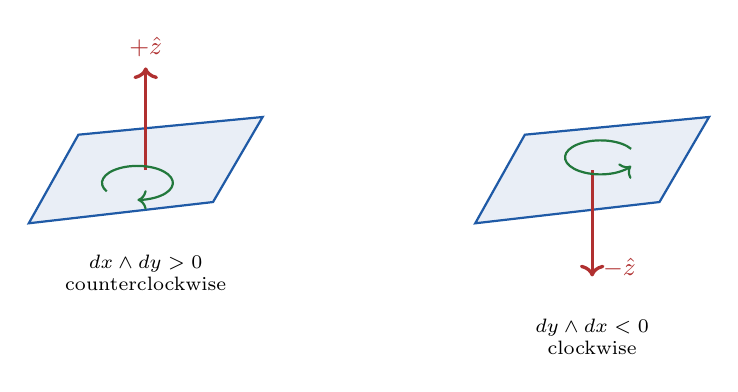
\begin{tikzpicture}[scale=0.9]
% Left: region with +z normal and ccw arrow
\begin{scope}[shift={(0,0)}]
\draw[thick, figB, fill=figB!10] (0,0) -- (2.6,0.3) -- (3.3,1.5) -- (0.7,1.25) -- cycle;
\draw[->, very thick, figR] (1.65,0.75) -- (1.65,2.2) node[above, font=\small] {$+\hat{z}$};
\draw[->, thick, figG] (1.1,0.45) arc[start angle=210, end angle=-90, x radius=0.5, y radius=0.24];
\node[font=\scriptsize, align=center] at (1.65,-0.7) {$dx \wedge dy > 0$\\ counterclockwise};
\end{scope}
% Right: same region with -z normal and cw arrow
\begin{scope}[shift={(6.3,0)}]
\draw[thick, figB, fill=figB!10] (0,0) -- (2.6,0.3) -- (3.3,1.5) -- (0.7,1.25) -- cycle;
\draw[->, very thick, figR] (1.65,0.75) -- (1.65,-0.75) node[right, font=\small, yshift=3pt] {$-\hat{z}$};
\draw[->, thick, figG] (2.2,1.05) arc[start angle=30, end angle=330, x radius=0.5, y radius=0.24];
\node[font=\scriptsize, align=center] at (1.65,-1.6) {$dy \wedge dx < 0$\\ clockwise};
\end{scope}
\end{tikzpicture}%
\figcap{Two descriptions of the same choice. Geometric: pick a normal direction. Algebraic: pick a coordinate ordering. Flipping the normal $\leftrightarrow$ swapping the order $\leftrightarrow$ negating $dx \wedge dy$.}
\end{center}

\textbf{In 1D:} There is only one coordinate $x$ --- nothing to swap it with. Instead, orientation is the \textbf{choice of direction}: does $x$ increase or decrease as you traverse? Writing $\int_a^b$ means ``traverse in the direction of increasing $x$'' (standard). Writing $\int_b^a$ means ``traverse in the direction of decreasing $x$'' (reversed). The sign flip $\int_a^b = -\int_b^a$ is the 1D version of switching the coordinate ordering. There is no second coordinate to swap, so the only freedom is the sign of the single basis vector: $+\hat{e}_x$ or $-\hat{e}_x$.

\textbf{The uniform description:} In all dimensions, orientation is determined by the \textbf{sign of the permutation} of basis vectors. Two ordered bases have the same orientation if and only if the permutation relating them is even (an even number of transpositions); they have opposite orientation if the permutation is odd. This is encoded by the Levi-Civita symbol $\varepsilon_{ij\ldots k}$, which equals $+1$ for even permutations, $-1$ for odd, and $0$ if any index is repeated.

In 1D, the only ``permutation'' is the sign of the single basis vector: $\{+\hat{e}_x\}$ vs $\{-\hat{e}_x\}$. In 2D, $\{\hat{e}_x, \hat{e}_y\}$ vs $\{\hat{e}_y, \hat{e}_x\}$ is a single transposition (odd, so orientation reverses). In 3D, even permutations of $\{\hat{e}_x, \hat{e}_y, \hat{e}_z\}$ --- such as $(y,z,x)$ and $(z,x,y)$ --- preserve orientation, while odd ones --- such as $(y,x,z)$ --- reverse it.

The wedge product $\wedge$ (defined formally in \S21; for now, the key property is $dx_i \wedge dx_j = -dx_j \wedge dx_i$, with $dx_i \wedge dx_i = 0$) is the realization of this same structure as an algebraic operation on differentials:
\[
dx_i \wedge dx_j \wedge dx_k = \varepsilon_{ijk}\,dx \wedge dy \wedge dz.
\]

The three defining properties match exactly: swapping two indices negates $\varepsilon_{ijk}$, and swapping two wedge factors negates the product; repeating an index gives $\varepsilon_{iik} = 0$, and $dx_i \wedge dx_i = 0$; the standard ordering gives $\varepsilon_{123} = +1$, and $dx \wedge dy \wedge dz > 0$. The determinant formula $\det(A) = \sum_\sigma \mathrm{sgn}(\sigma)\prod_i A_{i,\sigma(i)}$ is what you get when you expand the wedge product evaluated on a set of vectors --- the wedge product computes determinants by tracking permutation signs automatically.

So the cross product, the determinant, the Jacobian, and the wedge product are all manifestations of the same algebraic structure: \textbf{alternating multilinear maps}. The Levi-Civita symbol is the coordinate version; the wedge product is the coordinate-free version that works in any dimension and on any manifold. The geometric intuition (direction of traversal, normal vector) is available only when the region is embedded in a higher-dimensional space.

The pattern is: a $k$-dimensional region in $\R^n$ with $n > k$ has a \textbf{normal direction} in the ambient space, so orientation is geometric and visible. A $k$-dimensional region in $\R^k$ (top-dimensional) has no ambient space to point into, so orientation is purely algebraic.

\begin{center}
\renewcommand{\arraystretch}{1.4}
\begin{tabular}{|l|c|l|c|}
\hline
\textbf{Region} & \textbf{Top-dim?} & \textbf{Orientation means\ldots} & \textbf{Visible?} \\
\hline
Curve in $\R^2$ or $\R^3$ & no & direction of traversal & yes \\
\hline
Surface in $\R^2$ & yes & $(x,y)$ vs $(y,x)$ ordering & no \\
\hline
Surface in $\R^3$ & no & normal points up or down & yes \\
\hline
Volume in $\R^3$ & yes & $(x,y,z)$ vs $(y,x,z)$ ordering & no \\
\hline
Volume in $\R^4$ & no & normal points in $+w$ or $-w$ & yes \\
\hline
\end{tabular}
\end{center}

This is why surface orientation in $\R^3$ feels natural (you can point to the normal) but volume orientation in $\R^3$ feels abstract (there is no 4th dimension to point into). If you \textit{did} embed $\R^3$ into $\R^4$, a 3D region would suddenly have a normal direction ($\pm\hat{e}_w$), and the two orientations would become ``which side of the 3D hypersurface are you on'' --- exactly like the two sides of a surface in $\R^3$.

This also explains why the Divergence Theorem needs the \textit{boundary surface} to be oriented (the normal is visible --- outward vs inward) but does not need the \textit{volume itself} to be oriented (it is top-dimensional, so the standard orientation of $\R^3$ is automatic). And it is why $|J|$ suffices for volume integrals in this course: since everyone agrees on the standard coordinate ordering, the signed and unsigned versions always agree, and orientation is invisible.

\subsection{What a Differential Form Is}

\begin{definition}[Differential Form]
Let $x_1, \ldots, x_n$ be the standard coordinates on $\R^n$. The \textbf{coordinate 1-forms} $dx_1, \ldots, dx_n$ are defined by:
\[
dx_i(\mathbf{v}) = v_i \qquad \text{(the $i$-th component of $\mathbf{v}$)}.
\]
A \textbf{$k$-form} on an open subset $U \subseteq \R^n$ is an expression:
\[
\omega = \sum_{i_1 < i_2 < \cdots < i_k} f_{i_1 \cdots i_k}(x_1, \ldots, x_n) \; dx_{i_1} \wedge dx_{i_2} \wedge \cdots \wedge dx_{i_k},
\]
where each $f_{i_1 \cdots i_k}: U \to \R$ is a smooth coefficient function, and the sum runs over all $\binom{n}{k}$ strictly increasing index sequences.

The special cases are:
\begin{itemize}
    \item A \textbf{0-form} is a smooth function $f: U \to \R$.
    \item In $\R^3$: a \textbf{1-form} is $f_1\,dx + f_2\,dy + f_3\,dz$ (3 coefficients); a \textbf{2-form} is $f_{23}\,dy \wedge dz + f_{31}\,dz \wedge dx + f_{12}\,dx \wedge dy$ (3 coefficients); a \textbf{3-form} is $f_{123}\,dx \wedge dy \wedge dz$ (1 coefficient).
\end{itemize}
\end{definition}

\textbf{What this definition says, concretely:}

A $k$-form is a machine: at each point, you feed it $k$ tangent vectors and it outputs a number.

\textbf{0-form} (one coefficient). A smooth function $f(x,y,z)$. It eats zero tangent vectors --- it just outputs a number at each point. ``Integrating'' a 0-form means evaluating it: $\int_{\{p\}} f = f(p)$.

A 0-form needs only one coefficient because there is no direction to choose.

\textbf{1-form} (three coefficients in $\R^3$). At each point, it eats one tangent vector $\mathbf{v}$ and outputs a number. To do this, it needs to assign a weight to each independent direction: ``if you move in $dx$, the weight is $f_1$; in $dy$, it is $f_2$; in $dz$, it is $f_3$.'' So a 1-form in $\R^3$ has $\binom{3}{1} = 3$ coefficient functions:
\[
\omega = f_1\,dx + f_2\,dy + f_3\,dz.
\]

The coefficients $f_1, f_2, f_3$ are smooth functions of $(x,y,z)$ --- they vary from point to point. They are \textbf{coordinate-dependent}: in $(x,y,z)$ coordinates, $f_1(p) = \omega_p(\hat{e}_x)$ is ``what the form outputs when fed the unit vector in the $x$-direction.'' In spherical coordinates, the same form $\omega$ would have different coefficient functions, because the basis vectors $\hat{e}_r, \hat{e}_\theta, \hat{e}_\phi$ are different from $\hat{e}_x, \hat{e}_y, \hat{e}_z$. The form itself is coordinate-independent; the coefficients describe it in a particular coordinate system --- just as a vector field $\mathbf{F}$ has different components in Cartesian vs.\ spherical, but points in the same direction.

When you feed $\omega$ a tangent vector $\mathbf{v} = (v_1, v_2, v_3)$, the output is $f_1 v_1 + f_2 v_2 + f_3 v_3$. To integrate $\omega$ over a curve $\gamma$, you feed it the tangent vector $\gamma'(t)\,dt$ at each point and sum:
\[
\int_\gamma \omega = \int_a^b (f_1\, x' + f_2\, y' + f_3\, z')\,dt.
\]

(In \S15--\S19, we wrote $P, Q, R$ for $f_1, f_2, f_3$.)

The simplest 1-form is $df = f_x\,dx + f_y\,dy + f_z\,dz$, where the coefficients come from a single function $f$. But not every 1-form arises this way: $\omega = y\,dx + x^2\,dy$ has no single antiderivative $f$ with $f_x = y$ and $f_y = x^2$ (since $f_{xy} = 1 \neq 2x = f_{yx}$). Such a form is called \textit{not exact}.

This $df$ is the same object as the differential from \S8 --- same formula, same notation. In \S8, we introduced $df = f_x\,dx + f_y\,dy + f_z\,dz$ as the ``best linear approximation'': $\Delta f \approx f_x\,\Delta x + f_y\,\Delta y + f_z\,\Delta z$ for small changes. But we never said precisely what $dx$, $dy$, $dz$ \textit{are}. Now we can: $dx$ is the 1-form that eats a tangent vector $\mathbf{v} = (v_1, v_2, v_3)$ and outputs $v_1$ (the $x$-component). So $df$ eats $\mathbf{v}$ and outputs $f_x v_1 + f_y v_2 + f_z v_3 = \nabla f \cdot \mathbf{v}$, the directional derivative of $f$ in direction $\mathbf{v}$. The ``best linear approximation'' and the ``1-form that outputs directional derivatives'' are the same thing --- and this is where the name ``differential forms'' comes from: $df$ is the prototypical example, and all forms generalize it.

\textbf{2-form} (three coefficients in $\R^3$). At each point, it eats two tangent vectors (spanning a parallelogram) and outputs a signed area, weighted differently for each independent plane. In $\R^3$ there are $\binom{3}{2} = 3$ independent coordinate planes ($yz$, $zx$, $xy$), so a 2-form needs three coefficient functions:
\[
\eta = f_{23}\,dy \wedge dz + f_{31}\,dz \wedge dx + f_{12}\,dx \wedge dy.
\]

(In \S15--\S19, we wrote $A, B, C$ for $f_{23}, f_{31}, f_{12}$. The subscript notation makes the structure explicit: the subscripts name which basis element the coefficient multiplies.)

To integrate $\eta$ over a surface $S$ parametrized by $\mathbf{X}(u,v)$: at each point of $S$, the parametrization provides two tangent vectors $\mathbf{X}_u$ and $\mathbf{X}_v$ (from \S17). These span a small parallelogram --- the infinitesimal surface element. The 2-form eats this pair of vectors and outputs a number (the signed area, weighted by the coefficients at that point). Summing over all such parallelograms:
\[
\iint_S \eta = \iint_D \big[ f_{23}(y_u z_v - z_u y_v) + f_{31}(z_u x_v - x_u z_v) + f_{12}(x_u y_v - y_u x_v) \big] \, du \, dv.
\]

The three parenthesized terms are the components of $\mathbf{X}_u \times \mathbf{X}_v$, so this is $\iint_D (f_{23}, f_{31}, f_{12}) \cdot (\mathbf{X}_u \times \mathbf{X}_v) \, du\,dv$ --- the flux integral from \S17.

\textbf{3-form} (one coefficient in $\R^3$). At each point, it eats three tangent vectors (spanning a parallelepiped) and outputs signed volume times a coefficient. There is only $\binom{3}{3} = 1$ way to choose 3 differentials from $\{dx, dy, dz\}$: you must take all three. Any other combination either repeats a differential ($dx \wedge dx \wedge dy = 0$) or is a permutation of $dx \wedge dy \wedge dz$ (giving $\pm dx \wedge dy \wedge dz$). So a 3-form has just one coefficient:
\[
\mu = f_{123}\,dx \wedge dy \wedge dz.
\]

To integrate: if $V$ is described directly in $(x,y,z)$ coordinates, $\iiint_V \mu = \iiint_V f_{123}\,dx\,dy\,dz$. (In $\R^4$, a 3-form would have $\binom{4}{3} = 4$ terms.)

\textbf{The count of coefficients} follows Pascal's triangle: $\binom{3}{0} = 1$, $\binom{3}{1} = 3$, $\binom{3}{2} = 3$, $\binom{3}{3} = 1$. It rises then falls because choosing which 2 of 3 directions to include is the same as choosing which 1 to exclude.

\subsection{Forms and Riemann Integration}

Looking at the integration formulas above, you may notice: the right-hand side of every formula is an ordinary Riemann integral over a parameter domain. For instance:
\[
\int_\gamma \omega = \int_a^b (\underbrace{f_1\, x' + f_2\, y' + f_3\, z'}_{\text{a function of } t})\,dt, \qquad \iint_S \eta = \iint_D (\underbrace{(f_{23}, f_{31}, f_{12}) \cdot (\mathbf{X}_u \times \mathbf{X}_v)}_{\text{a function of } (u,v)})\,du\,dv.
\]

So what did the form actually \textit{do}? It produced the correct integrand. The form $\omega = f_1\,dx + f_2\,dy + f_3\,dz$, combined with the parametrization $\gamma(t)$, automatically generated the function $f_1 x' + f_2 y' + f_3 z'$ that goes inside the Riemann integral. Without forms, you derive this by hand (chain rule, cross products, Jacobians). With forms, the pullback machinery does it for you.

The two layers do different jobs:
\begin{itemize}
    \item \textbf{Forms} (this section) determine \textit{what} to integrate: the correct integrand on the parameter domain, with all Jacobians and signs.
    \item \textbf{Riemann integration} (\S14) determines the \textit{number}: Riemann sums, Fubini, etc.
\end{itemize}

Forms do not replace Riemann integration. They sit on top of it. On flat domains in Cartesian coordinates, you can skip the forms layer entirely --- the Riemann integral works directly. This is what we did for 90\% of the course. The forms layer becomes essential when the domain is curved (curves, surfaces), the coordinates are non-Cartesian (polar, spherical), or you want to understand why three integral theorems are really one theorem.

\textbf{The 1D inconsistency resolved.}

We can now return to the inconsistency from the three categories above. In the forms framework, the change of variables in \textit{every} dimension uses the signed Jacobian:
\[
\iint_D f\,dx \wedge dy = \iint_{D^*} f(\Phi) \cdot J\,du \wedge dv.
\]

Consider two parametrizations of the same region $D$: one with $\Phi(u,v)$ (where $J > 0$), and another $\tilde{\Phi}(u,v) = \Phi(v,u)$ that swaps the parameter roles (so $\tilde{J} = -J < 0$). These describe the same geometric region, but with opposite orientations. The forms formula gives:
\[
\iint_{D^*} f(\Phi) \cdot J\,du\,dv \quad \text{vs.} \quad \iint_{D^*} f(\tilde{\Phi}) \cdot (-J)\,du\,dv.
\]

The sign flip in the Jacobian reflects the orientation reversal --- exactly as in 1D, where going from $a$ to $b$ vs.\ $b$ to $a$ produces opposite signs. The $|J|$ approach from \S15 gives $|J| = |-J|$, so both parametrizations yield the same positive number. This is correct for computing areas, but it means the integral cannot distinguish the two orientations --- which is exactly the information the integral theorems need.

\begin{remark}[Riemann vs.\ Lebesgue]
The two-layer picture above shows that the forms layer (pullback, wedge products, Jacobians) is purely algebraic --- it does not depend on which integration theory computes the number in step 2. Everything in these notes uses the Riemann integral, but the forms framework works identically with the Lebesgue integral from \S15 of the 551 notes. For continuous functions on compact domains, the two integrals agree (one of the first results in 551), so every computation here gives the same answer either way. The Lebesgue integral becomes necessary when pushing beyond 452: forms with $L^p$ coefficients (not just smooth), limit theorems (DCT/MCT for swapping $\lim$ and $\int$), and Hodge theory (minimizing $L^2$ norms over spaces of forms). The forms framework is the same; the integration backend determines how far you can push it.
\end{remark}

\subsection{Why the Algebra Must Be Anti-Commutative}

We have said that a $k$-form ``waits for a parametrization'' to become a number. But what algebra governs the combination of differentials? The answer is not imposed by convention --- it is \textit{forced} by the requirement that coordinate substitution reproduces the Jacobian determinant.

\subsection*{Discovering the Rules from a Computation}

Consider a surface $\mathbf{X}(u,v) = (x(u,v), y(u,v))$ in $\R^2$. We want to express the area element $dx\,dy$ in terms of $du\,dv$.

\textbf{Step 1.} The chain rule gives:
\[
dx = x_u\,du + x_v\,dv, \qquad dy = y_u\,du + y_v\,dv.
\]

\textbf{Step 2.} Combine these into an area element. Expand formally, treating the product of differentials as an unknown operation:
\[
(x_u\,du + x_v\,dv)(y_u\,du + y_v\,dv) = x_u y_u\,du\,du + x_u y_v\,du\,dv + x_v y_u\,dv\,du + x_v y_v\,dv\,dv.
\]

\textbf{Step 3.} We know from \S15 that the correct answer is the \textit{signed} Jacobian determinant:
\[
(x_u y_v - x_v y_u)\,du\,dv = \det \begin{pmatrix} x_u & x_v \\ y_u & y_v \end{pmatrix} du\,dv.
\]

For the expansion in Step 2 to equal this, we \textit{need}:
\[
du\,du = 0, \qquad dv\,dv = 0, \qquad dv\,du = -du\,dv.
\]

These are not arbitrary conventions --- they are forced by the determinant:
\begin{itemize}
    \item $du\,du = 0$: If we tried to compute $dx \wedge dx$ by the same method, we would get $\det\begin{pmatrix} x_u & x_u \\ x_v & x_v \end{pmatrix} = 0$ --- a determinant with two identical columns is always zero. So the ``product of $dx$ with itself'' must vanish.
    \item $dv\,du = -du\,dv$: Swapping the two columns of a $2 \times 2$ determinant negates it: $\det\begin{pmatrix} x_u & x_v \\ y_u & y_v \end{pmatrix} = -\det\begin{pmatrix} x_v & x_u \\ y_v & y_u \end{pmatrix}$. Swapping $u \leftrightarrow v$ in the parametrization reverses the orientation, so the product of differentials must be anti-commutative.
\end{itemize}

\textbf{Step 4.} These are exactly the rules of the wedge product: $du \wedge du = 0$, $dv \wedge dv = 0$, and $dv \wedge du = -du \wedge dv$. The anti-commutativity is not an abstract axiom --- it is the \textit{unique} multiplication rule on differentials that makes coordinate substitution produce the Jacobian determinant.

\begin{center}
\includegraphics[width=0.60\textwidth]{pyfigs/f10_projection.pdf}%
\figcap{Each 2-form pullback is a signed projected area: $dx \wedge dy$ measures the shadow of the tangent parallelogram on the $xy$-plane, with sign given by orientation. The three shadows (on the $yz$-, $zx$-, $xy$-planes) are the three components of $\mathbf{X}_u \times \mathbf{X}_v$; the Gram determinant $\det(G)$ is the sum of their squares.}
\end{center}

The computation above is informal: we have not yet defined the wedge product. In \S22.1, we axiomatize these rules, and then the computation becomes a formal proposition (the \textit{pullback formula}) that underlies all integration of forms.

\section{The Algebra of Differential Forms}

\subsection{The Wedge Product}

In \S21.6, we discovered that coordinate substitution \textit{forces} the multiplication of differentials to be anti-commutative. We now axiomatize these rules.

\begin{note}[Terminology: Properties of Operations]
An \textbf{operation} takes two inputs and produces one output (like $+$ or $\times$). We say an operation $\star$ is:

\textbf{Linear in the first argument} if $(\alpha a + \beta b) \star c = \alpha (a \star c) + \beta (b \star c)$ for all scalars $\alpha, \beta$. That is, the operation distributes over addition and commutes with scalar multiplication --- just like ordinary multiplication does.

\textbf{Bilinear} if it is linear in each argument separately: linear in the first when the second is held fixed, and linear in the second when the first is held fixed. The dot product $\mathbf{u} \cdot \mathbf{v}$ and the cross product $\mathbf{u} \times \mathbf{v}$ are both bilinear. (You already use this implicitly every time you expand $(a\mathbf{u} + b\mathbf{v}) \times \mathbf{w} = a(\mathbf{u} \times \mathbf{w}) + b(\mathbf{v} \times \mathbf{w})$.)

\textbf{Associative} if $(a \star b) \star c = a \star (b \star c)$, so parentheses don't matter. Addition and multiplication are associative; the cross product is \textit{not} ($(\mathbf{u} \times \mathbf{v}) \times \mathbf{w} \neq \mathbf{u} \times (\mathbf{v} \times \mathbf{w})$ in general).

\textbf{Commutative} if $a \star b = b \star a$. \textbf{Anti-commutative} if $a \star b = -(b \star a)$. The cross product is anti-commutative; the wedge product will be too.
\end{note}

\begin{definition}[Wedge Product]
The wedge product is an operation on forms satisfying three rules:

\begin{enumerate}
    \item \textbf{Anti-commutativity:} $dx_i \wedge dx_j = -dx_j \wedge dx_i$ for any coordinate differentials.
    \item \textbf{Linearity in each factor:} $(a\,\omega_1 + b\,\omega_2) \wedge \eta = a\,(\omega_1 \wedge \eta) + b\,(\omega_2 \wedge \eta)$, and similarly in the second factor. (This means you can expand wedge products using the distributive law, just like ordinary multiplication.)
    \item \textbf{Associativity:} $(\omega \wedge \eta) \wedge \mu = \omega \wedge (\eta \wedge \mu)$.
\end{enumerate}

The key rule is:
\[
\boxed{dx_i \wedge dx_j = -dx_j \wedge dx_i}
\]

In particular, setting $i = j$: $dx_i \wedge dx_i = -dx_i \wedge dx_i$, which forces $dx_i \wedge dx_i = 0$.
\end{definition}

\textbf{Why anti-commutativity?} This encodes \textbf{orientation}. Recall:
\begin{itemize}
    \item Swapping the order of parameters in a cross product flips the sign: $\mathbf{X}_u \times \mathbf{X}_v = -\mathbf{X}_v \times \mathbf{X}_u$.
    \item Changing the order of integration in a signed integral flips the sign: $\int_a^b = -\int_b^a$.
    \item The Jacobian determinant changes sign when two rows (or columns) are swapped.
\end{itemize}

All of these are manifestations of the same algebraic fact: $dx \wedge dy = -dy \wedge dx$. The wedge product is the single operation that captures orientation.

\textbf{Consequences:}

\textit{1. Any repeated factor kills the product:} $dx \wedge dx = -dx \wedge dx = 0$.

\textit{2. In $\R^3$, there are exactly 3 independent 2-forms:} $dy \wedge dz$, $dz \wedge dx$, $dx \wedge dy$. All others are either zero ($dx \wedge dx = 0$) or related by anti-commutativity ($dz \wedge dy = -dy \wedge dz$).

\textit{3. There is exactly one independent 3-form:} $dx \wedge dy \wedge dz$. Any permutation of the factors gives $\pm dx \wedge dy \wedge dz$ (the sign is the sign of the permutation).

\textit{4. In $\R^n$, there are $\binom{n}{k}$ independent $k$-forms:} choose which $k$ of the $n$ coordinate differentials appear. In $\R^3$: $\binom{3}{0} = 1$ function, $\binom{3}{1} = 3$ one-forms, $\binom{3}{2} = 3$ two-forms, $\binom{3}{3} = 1$ three-form.

\begin{definition}[Levi-Civita Symbol]
For indices $i_1, i_2, \ldots, i_k \in \{1, 2, \ldots, n\}$, the \textbf{Levi-Civita symbol} is:
\[
\varepsilon_{i_1 i_2 \cdots i_k} = \begin{cases} +1 & \text{if } (i_1, \ldots, i_k) \text{ is an even permutation of } (1, 2, \ldots, k), \\ -1 & \text{if } (i_1, \ldots, i_k) \text{ is an odd permutation of } (1, 2, \ldots, k), \\ 0 & \text{if any index is repeated.} \end{cases}
\]
\end{definition}

\begin{proposition}[Wedge Product Equals Levi-Civita Symbol]
For coordinate differentials $dx_i, dx_j$ in $\R^n$:
\[
dx_i \wedge dx_j = \varepsilon_{ij}\,dx \wedge dy \quad (\text{in } \R^2), \qquad dx_i \wedge dx_j \wedge dx_k = \varepsilon_{ijk}\,dx \wedge dy \wedge dz \quad (\text{in } \R^3).
\]
More generally, $dx_{i_1} \wedge \cdots \wedge dx_{i_k} = \varepsilon_{i_1 \cdots i_k}\,dx_1 \wedge \cdots \wedge dx_k$.
\end{proposition}

\begin{proof}
Both sides obey the same rules: (i) swapping two adjacent factors/indices negates the value (anti-commutativity of $\wedge$ and the sign rule for $\varepsilon$), and (ii) a repeated factor/index gives zero ($dx_i \wedge dx_i = 0$ and $\varepsilon_{\ldots i \ldots i \ldots} = 0$). Since both sides equal $+1$ on the identity permutation ($dx_1 \wedge \cdots \wedge dx_k$ and $\varepsilon_{12\ldots k} = 1$), they agree everywhere.
\end{proof}

The wedge product is the Levi-Civita symbol promoted from a numerical table to an algebraic operation.

\begin{example}[Computing with Wedge Products]
Let $\omega = x \, dy + y \, dz$ (a 1-form) and $\eta = z \, dx + x \, dy$ (a 1-form). Their wedge product is a 2-form:
\begin{align*}
\omega \wedge \eta &= (x \, dy + y \, dz) \wedge (z \, dx + x \, dy) \\
&= xz \, dy \wedge dx + x^2 \, dy \wedge dy + yz \, dz \wedge dx + xy \, dz \wedge dy \\
&= -xz \, dx \wedge dy + 0 + yz \, dz \wedge dx - xy \, dy \wedge dz \\
&= -xy \, dy \wedge dz + yz \, dz \wedge dx - xz \, dx \wedge dy.
\end{align*}
\end{example}

We can now formalize the computation from \S21.6. The key concept is the \textit{pullback}: the operation that translates a form from ambient coordinates to parameter coordinates so that it can be integrated.

\begin{definition}[Pullback]
Let $\omega$ be a differential form on $\R^n$, expressed in the \textbf{ambient coordinates} $x_1, \ldots, x_n$.

Let $\Phi: D \subseteq \R^k \to \R^n$ be a $C^1$ map (a \textbf{parametrization}), where $D$ has its own \textbf{parameter coordinates} $u_1, \ldots, u_k$. The map $\Phi$ relates the two coordinate systems:
\[
\Phi(u_1, \ldots, u_k) = \big(x_1(u_1, \ldots, u_k),\; \ldots,\; x_n(u_1, \ldots, u_k)\big).
\]

The \textbf{pullback} $\Phi^*\omega$ is the form on $D$ obtained by:
\begin{enumerate}
    \item Replacing each ambient differential $dx_i$ with $\displaystyle\sum_{j=1}^k \parti{x_i}{u_j}\,du_j$ (the chain rule),
    \item Expanding using the wedge product rules.
\end{enumerate}

The integral of $\omega$ over $\Phi(D)$ is then defined as:
\[
\int_{\Phi(D)} \omega \;=\; \int_D \Phi^*\omega.
\]
\end{definition}

\begin{center}
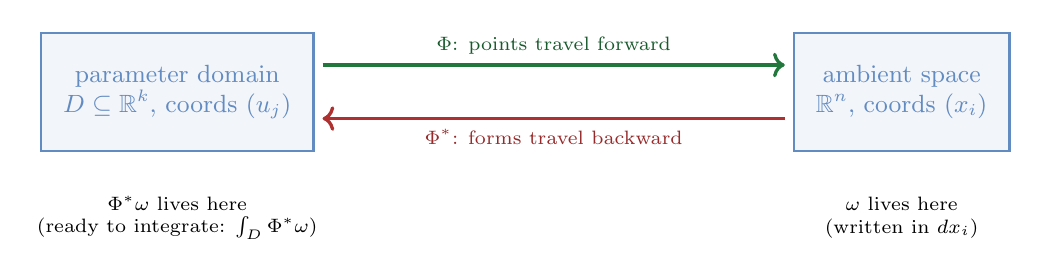
\begin{tikzpicture}[scale=1.0]
% left box: parameter domain
\node[draw, thick, figB!70, fill=figB!6, minimum height=1.5cm, align=center, font=\small, inner xsep=8pt] (Dbox) at (0,0) {parameter domain\\ $D \subseteq \R^k$, coords $(u_j)$};
% right box: ambient space
\node[draw, thick, figB!70, fill=figB!6, minimum height=1.5cm, align=center, font=\small, inner xsep=8pt] (Rbox) at (9.2,0) {ambient space\\ $\R^n$, coords $(x_i)$};
% forward arrow: points
\draw[->, very thick, figG] ($(Dbox.east)+(0.1,0.34)$) -- ($(Rbox.west)+(-0.1,0.34)$)
  node[midway, above, font=\scriptsize, figG!75!black] {$\Phi$: points travel forward};
% backward arrow: forms
\draw[<-, very thick, figR] ($(Dbox.east)+(0.1,-0.34)$) -- ($(Rbox.west)+(-0.1,-0.34)$)
  node[midway, below, font=\scriptsize, figR!85!black] {$\Phi^*$: forms travel backward};
% annotations under each box
\node[font=\scriptsize, align=center] at (0,-1.6) {$\Phi^*\omega$ lives here\\ (ready to integrate: $\int_D \Phi^*\omega$)};
\node[font=\scriptsize, align=center] at (9.2,-1.6) {$\omega$ lives here\\ (written in $dx_i$)};
\end{tikzpicture}%
\figcap{The two directions of the pullback story. The parametrization $\Phi$ pushes points forward: $(u,v) \mapsto \mathbf{X}(u,v)$. The pullback $\Phi^*$ pulls forms backward: a form written in ambient differentials $dx_i$ becomes a form in parameter differentials $du_j$, via $dx_i = \sum_j (x_i)_{u_j}\,du_j$. Integration always happens at the parameter end --- $\int_{\Phi(D)}\omega$ is \textnormal{defined} as $\int_D \Phi^*\omega$.}
\end{center}


\begin{remark}[Clarification of Terms]
The ambient coordinates $(x_1, \ldots, x_n)$ are the standard coordinates on $\R^n$ --- the space the form lives in. The parameter coordinates $(u_1, \ldots, u_k)$ are the coordinates on $D$ --- the space we integrate over. The parametrization $\Phi$ is the bridge: it tells us, for each point in $D$, where it sits in $\R^n$. You have been using parametrizations all semester:
\begin{center}
\renewcommand{\arraystretch}{1.4}
\begin{tabular}{|l|l|c|c|l|l|}
\hline
\textbf{Object} & \textbf{$\Phi$} & $k$ & $n$ & \textbf{Parameter coords} & \textbf{Ambient coords} \\
\hline
Curve in $\R^3$ & $\boldsymbol{\gamma}(t)$ & 1 & 3 & $t$ & $(x,y,z)$ \\
\hline
Surface in $\R^3$ & $\mathbf{X}(u,v)$ & 2 & 3 & $(u,v)$ & $(x,y,z)$ \\
\hline
Polar coords & $(r\cos\theta, r\sin\theta)$ & 2 & 2 & $(r,\theta)$ & $(x,y)$ \\
\hline
Spherical coords & $(r\sin\phi\cos\theta, \ldots)$ & 3 & 3 & $(r,\theta,\phi)$ & $(x,y,z)$ \\
\hline
\end{tabular}
\end{center}
The pullback is what you compute every time you ``substitute the parametrization into the integral'' --- now given a name and a systematic procedure.
\end{remark}

\textbf{Carrying out the pullback} produces determinants of minors of the Jacobian matrix $J = \big[\parti{x_i}{u_j}\big]$ (which is $n \times k$):

\[
\Phi^*(dx_{i_1} \wedge \cdots \wedge dx_{i_k}) = \det \begin{pmatrix} (x_{i_1})_{u_1} & \cdots & (x_{i_1})_{u_k} \\ \vdots & \ddots & \vdots \\ (x_{i_k})_{u_1} & \cdots & (x_{i_k})_{u_k} \end{pmatrix} du_1 \wedge \cdots \wedge du_k.
\]

That is, the pullback of a coordinate $k$-form extracts the $k \times k$ minor of $J$ corresponding to rows $i_1, \ldots, i_k$. This is not a new result --- it is what happens when you carry out steps 1 and 2 of the definition. Each $dx_{i_\ell}$ becomes $\sum_j (x_{i_\ell})_{u_j}\,du_j$; wedging $k$ of these and using anti-commutativity kills all terms with repeated $du_j$; the surviving terms are the Leibniz formula for the determinant (as shown in the proof in \S21.6).

\begin{example}[Pullback Along a Curve (Line Integral, \S16)]
Let $\omega = f_1\,dx + f_2\,dy + f_3\,dz$ be a 1-form on $\R^3$, and $\boldsymbol{\gamma}: [a,b] \to \R^3$ a curve with $\boldsymbol{\gamma}(t) = (x(t), y(t), z(t))$.

The Jacobian is $3 \times 1$: $J = \begin{pmatrix} x' \\ y' \\ z' \end{pmatrix}$. Pull back:
\[
\boldsymbol{\gamma}^*\omega = f_1\,x'\,dt + f_2\,y'\,dt + f_3\,z'\,dt = (f_1 x' + f_2 y' + f_3 z')\,dt.
\]
So:
\[
\int_{\boldsymbol{\gamma}} \omega = \int_a^b (f_1 x' + f_2 y' + f_3 z')\,dt.
\]
This is the line integral $\int_{\boldsymbol{\gamma}} \mathbf{F} \cdot d\mathbf{r}$ from \S16.
\end{example}

\begin{example}[Pullback Along a Surface (Flux Integral, \S18)]
Let $\eta = f_{23}\,dy \wedge dz + f_{31}\,dz \wedge dx + f_{12}\,dx \wedge dy$ be a 2-form on $\R^3$, and $\mathbf{X}: D \to \R^3$ a surface with $\mathbf{X}(u,v) = (x(u,v), y(u,v), z(u,v))$.

The Jacobian is $3 \times 2$: $J = \begin{pmatrix} x_u & x_v \\ y_u & y_v \\ z_u & z_v \end{pmatrix}$. The three $2 \times 2$ minors give:
\begin{align*}
\mathbf{X}^*(dy \wedge dz) &= (y_u z_v - z_u y_v)\,du\,dv, \\
\mathbf{X}^*(dz \wedge dx) &= (z_u x_v - x_u z_v)\,du\,dv, \\
\mathbf{X}^*(dx \wedge dy) &= (x_u y_v - y_u x_v)\,du\,dv.
\end{align*}
So:
\[
\iint_S \eta = \iint_D \big[f_{23}(y_u z_v - z_u y_v) + f_{31}(z_u x_v - x_u z_v) + f_{12}(x_u y_v - y_u x_v)\big]\,du\,dv.
\]
The three parenthesized quantities are the components of $\mathbf{X}_u \times \mathbf{X}_v$, so this is $\iint_D \mathbf{F} \cdot (\mathbf{X}_u \times \mathbf{X}_v)\,du\,dv$ --- the flux integral from \S18.
\end{example}

\begin{example}[Pullback for Change of Variables (\S15)]
Let $\mu = f\,dx \wedge dy$ be a 2-form on $\R^2$, and $\Phi: D^* \to \R^2$ a coordinate change with $\Phi(u,v) = (x(u,v), y(u,v))$.

The Jacobian is $2 \times 2$: $J = \begin{pmatrix} x_u & x_v \\ y_u & y_v \end{pmatrix}$. There is $\binom{2}{2} = 1$ minor --- the full determinant:
\[
\Phi^*(dx \wedge dy) = (x_u y_v - x_v y_u)\,du \wedge dv = (\det J)\,du\,dv.
\]
So:
\[
\iint_D f\,dx\,dy = \iint_{D^*} f(\Phi(u,v)) \cdot (\det J)\,du\,dv.
\]
This is the \textit{signed} change of variables formula. The $|J|$ version from \S15 takes the absolute value, discarding the orientation (Category 3).
\end{example}

\begin{remark}[The Cross Product Is the Pullback in Disguise]
In $\R^3$, the three $2 \times 2$ minors of the Jacobian are exactly the three components of the cross product:
\[
\mathbf{X}_u \times \mathbf{X}_v = \big(\underbrace{y_u z_v - z_u y_v}_{\mathbf{X}^*(dy \wedge dz)}, \;\; \underbrace{z_u x_v - x_u z_v}_{\mathbf{X}^*(dz \wedge dx)}, \;\; \underbrace{x_u y_v - y_u x_v}_{\mathbf{X}^*(dx \wedge dy)}\big).
\]
The cross product packages the pullbacks of all three coordinate 2-forms into a single vector. This packaging only works in $\R^3$, because $\binom{3}{2} = 3$: the number of independent 2-forms equals the dimension. In $\R^4$ there would be $\binom{4}{2} = 6$ minors --- not packageable as a vector. The pullback works in any dimension; the cross product is its $\R^3$ shortcut.
\end{remark}

\subsection{The Exterior Derivative}

The exterior derivative $d$ takes a $k$-form to a $(k+1)$-form. It is defined by a simple recipe and turns out to unify the gradient, curl, and divergence.

\begin{definition}[Exterior Derivative]
\

\textbf{On 0-forms} (functions $f$):
\[
df = \parti{f}{x} dx + \parti{f}{y} dy + \parti{f}{z} dz.
\]

This is the total differential from Section 8 --- the same $df$ we have been writing all semester.

\textbf{On 1-forms} ($\omega = f_1 \, dx + f_2 \, dy + f_3 \, dz$): apply $d$ to each coefficient and wedge with the existing differential:
\[
d\omega = df_1 \wedge dx + df_2 \wedge dy + df_3 \wedge dz
\]
where $df_1 = (f_1)_x \, dx + (f_1)_y \, dy + (f_1)_z \, dz$, etc.

\textbf{On 2-forms} ($\eta = f_{23} \, dy \wedge dz + f_{31} \, dz \wedge dx + f_{12} \, dx \wedge dy$): same rule:
\[
d\eta = df_{23} \wedge dy \wedge dz + df_{31} \wedge dz \wedge dx + df_{12} \wedge dx \wedge dy.
\]
\end{definition}

The recipe is always the same: differentiate each coefficient, wedge the result with the existing differentials, and simplify using anti-commutativity.

\begin{proposition}[$d$ on 0-Forms Gives the Gradient]
For a smooth function $f$ on $\R^3$:
\[
df = f_x \, dx + f_y \, dy + f_z \, dz.
\]
That is, the coefficients of the 1-form $df$ are the components of $\nabla f = (f_x, f_y, f_z)$. The differential from \S8 and the gradient from \S7 are the same object: one is a 1-form, the other is the corresponding vector field.
\end{proposition}

\begin{proposition}[$d$ on 1-Forms Gives the Curl]
For a smooth 1-form $\omega = f_1 \, dx + f_2 \, dy + f_3 \, dz$ on $\R^3$:
\[
d\omega = \big((f_3)_y - (f_2)_z\big) \, dy \wedge dz + \big((f_1)_z - (f_3)_x\big) \, dz \wedge dx + \big((f_2)_x - (f_1)_y\big) \, dx \wedge dy.
\]
That is, the coefficients of the 2-form $d\omega$ are the components of $\nabla \times \mathbf{F}$ where $\mathbf{F} = (f_1, f_2, f_3)$ (written $P, Q, R$ in \S16--\S20). The curl, first introduced in \S11 and \S16, is $d$ applied to a 1-form.
\end{proposition}

\begin{proof}
Compute:
\begin{align*}
d\omega &= df_1 \wedge dx + df_2 \wedge dy + df_3 \wedge dz \\
&= ((f_1)_x \, dx + (f_1)_y \, dy + (f_1)_z \, dz) \wedge dx + ((f_2)_x \, dx + (f_2)_y \, dy + (f_2)_z \, dz) \wedge dy \\
&\quad + ((f_3)_x \, dx + (f_3)_y \, dy + (f_3)_z \, dz) \wedge dz.
\end{align*}

Expanding, using $dx \wedge dx = dy \wedge dy = dz \wedge dz = 0$:
\begin{align*}
d\omega &= (f_1)_y \, dy \wedge dx + (f_1)_z \, dz \wedge dx \\
&\quad + (f_2)_x \, dx \wedge dy + (f_2)_z \, dz \wedge dy \\
&\quad + (f_3)_x \, dx \wedge dz + (f_3)_y \, dy \wedge dz.
\end{align*}

Using anti-commutativity to put each term in standard order ($dy \wedge dz$, $dz \wedge dx$, $dx \wedge dy$):
\[
d\omega = \big((f_3)_y - (f_2)_z\big) \, dy \wedge dz + \big((f_1)_z - (f_3)_x\big) \, dz \wedge dx + \big((f_2)_x - (f_1)_y\big) \, dx \wedge dy.
\]

The three coefficients are exactly the components of $\nabla \times \mathbf{F}$.
\end{proof}

\begin{proposition}[$d$ on 2-Forms Gives the Divergence]
For a smooth 2-form $\eta = f_{23} \, dy \wedge dz + f_{31} \, dz \wedge dx + f_{12} \, dx \wedge dy$ on $\R^3$:
\[
d\eta = \big((f_{23})_x + (f_{31})_y + (f_{12})_z\big) \, dx \wedge dy \wedge dz.
\]
That is, the coefficient of the 3-form $d\eta$ is $\nabla \cdot \mathbf{F}$ where $\mathbf{F} = (f_{23}, f_{31}, f_{12})$ (written $A, B, C$ in \S16--\S20). The divergence, first introduced in \S11 and \S16, is $d$ applied to a 2-form.
\end{proposition}

\begin{proof}
Compute:
\begin{align*}
d\eta &= df_{23} \wedge dy \wedge dz + df_{31} \wedge dz \wedge dx + df_{12} \wedge dx \wedge dy \\
&= ((f_{23})_x \, dx + (f_{23})_y \, dy + (f_{23})_z \, dz) \wedge dy \wedge dz \\
&\quad + ((f_{31})_x \, dx + (f_{31})_y \, dy + (f_{31})_z \, dz) \wedge dz \wedge dx \\
&\quad + ((f_{12})_x \, dx + (f_{12})_y \, dy + (f_{12})_z \, dz) \wedge dx \wedge dy.
\end{align*}

In each line, only the term with the ``missing'' differential survives (all others have a repeated factor):
\begin{align*}
d\eta &= (f_{23})_x \, dx \wedge dy \wedge dz + (f_{31})_y \, dy \wedge dz \wedge dx + (f_{12})_z \, dz \wedge dx \wedge dy.
\end{align*}

Reorder each to the standard $dx \wedge dy \wedge dz$ (each is an even permutation):
\[
d\eta = \big((f_{23})_x + (f_{31})_y + (f_{12})_z\big) \, dx \wedge dy \wedge dz.
\]

The coefficient is $\nabla \cdot \mathbf{F}$.
\end{proof}

These three propositions are summarized in the following table:
\begin{center}
\renewcommand{\arraystretch}{1.5}
\begin{tabular}{|c|c|c|c|}
\hline
\textbf{Input} & \textbf{Output} & \textbf{$d$ computes} & \textbf{Vector calculus name} \\
\hline
0-form $f$ & 1-form $df$ & $\nabla f$ & gradient \\
\hline
1-form $\omega$ & 2-form $d\omega$ & $\nabla \times \mathbf{F}$ & curl \\
\hline
2-form $\eta$ & 3-form $d\eta$ & $\nabla \cdot \mathbf{F}$ & divergence \\
\hline
\end{tabular}
\end{center}

\subsection*{The Ladder: Gradient, Curl, and Divergence Are Not at the Same Level}

In vector calculus, gradient, curl, and divergence all appear to be ``differential operators on vector fields'':
\[
f \xrightarrow{\nabla} \mathbf{F} \xrightarrow{\nabla\times} \mathbf{G} \xrightarrow{\nabla\cdot} h.
\]

It seems like curl and divergence sit at the same level --- both take vector fields and produce something. The identities $\nabla \times (\nabla f) = \mathbf{0}$ and $\nabla \cdot (\nabla \times \mathbf{F}) = 0$ look like two separate facts.

In the forms picture, they form a \textbf{ladder}:
\[
\underbrace{f}_{\text{0-form}} \xrightarrow{\;d\;} \underbrace{P\,dx + Q\,dy + R\,dz}_{\text{1-form}} \xrightarrow{\;d\;} \underbrace{A\,dy \wedge dz + B\,dz \wedge dx + C\,dx \wedge dy}_{\text{2-form}} \xrightarrow{\;d\;} \underbrace{h\,dx \wedge dy \wedge dz}_{\text{3-form}}
\]

Each arrow is the \textit{same} operator $d$, but applied at a different rung:
\begin{itemize}
    \item $d$ on a 0-form (degree $0 \to 1$) = gradient
    \item $d$ on a 1-form (degree $1 \to 2$) = curl
    \item $d$ on a 2-form (degree $2 \to 3$) = divergence
\end{itemize}

Curl and divergence are \textbf{not} at the same level: curl goes from degree 1 to degree 2, divergence goes from degree 2 to degree 3. The two ``separate'' identities $\nabla \times (\nabla f) = 0$ and $\nabla \cdot (\nabla \times \mathbf{F}) = 0$ are the single identity $d \circ d = 0$ applied at consecutive rungs.

\begin{remark}[The $\R^3$ Accident]
Why do curl and divergence \textit{look} like they are at the same level in vector calculus? Because of a coincidence specific to $\R^3$.

In $\R^n$, the number of independent $k$-forms is $\binom{n}{k}$. In $\R^3$:
\[
\binom{3}{0} = 1, \qquad \binom{3}{1} = 3, \qquad \binom{3}{2} = 3, \qquad \binom{3}{3} = 1.
\]

Both 1-forms and 2-forms have \textbf{3 components}. Since a vector field in $\R^3$ also has 3 components, we can represent \textit{both} as vector fields. This lets us write both curl and divergence as operations on ``vector fields,'' hiding the fact that they act on forms of different degrees.

\textbf{This coincidence fails in every other dimension:}
\begin{itemize}
    \item In $\R^2$: $\binom{2}{1} = 2$ components for 1-forms, $\binom{2}{2} = 1$ component for 2-forms. The ``curl'' of a 1-form $P\,dx + Q\,dy$ is the 2-form $(Q_x - P_y)\,dx \wedge dy$ --- a single scalar, not a vector. This is why the 2D curl in Green's theorem is a number, not a vector field.
    \item In $\R^4$: $\binom{4}{1} = 4$ components for 1-forms, $\binom{4}{2} = 6$ components for 2-forms. The ``curl'' of a 1-form is a 6-component object --- it cannot be represented as a vector field. The cross product does not exist in $\R^4$ for the same reason.
\end{itemize}

The exterior derivative $d$ works in \textit{any} dimension. The vector calculus operators grad, curl, div are dimension-3 translations of $d$ that rely on the coincidence $\binom{3}{1} = \binom{3}{2}$.

This also explains a fact from physics: the electromagnetic field in 4D spacetime is naturally a 2-form $F$ (with 6 independent components: 3 for $\mathbf{E}$, 3 for $\mathbf{B}$). Maxwell's equations become $dF = 0$ and $d{*}F = J$. The fact that $\mathbf{E}$ and $\mathbf{B}$ combine into a single object is invisible in 3D vector calculus but natural in the language of forms.
\end{remark}

\subsection{$d^2 = 0$: The Unifying Identity}

\begin{theorem}[$d^2 = 0$]
For any smooth $k$-form $\omega$: $d(d\omega) = 0$.
\end{theorem}

\begin{proof}
It suffices to check on a 0-form $f$ (the general case follows by linearity and the product rule).

Compute $d(df)$: we have $df = f_x \, dx + f_y \, dy + f_z \, dz$, so:
\begin{align*}
d(df) &= (f_{xy} \, dy + f_{xz} \, dz) \wedge dx + (f_{yx} \, dx + f_{yz} \, dz) \wedge dy + (f_{zx} \, dx + f_{zy} \, dy) \wedge dz \\
&= f_{xy} \, dy \wedge dx + f_{xz} \, dz \wedge dx + f_{yx} \, dx \wedge dy + f_{yz} \, dz \wedge dy \\
&\quad + f_{zx} \, dx \wedge dz + f_{zy} \, dy \wedge dz.
\end{align*}

Using $dy \wedge dx = -dx \wedge dy$, etc.:
\[
d(df) = (f_{yx} - f_{xy}) \, dx \wedge dy + (f_{xz} - f_{zx}) \, dz \wedge dx + (f_{zy} - f_{yz}) \, dy \wedge dz = 0
\]
by equality of mixed partials ($f_{xy} = f_{yx}$, etc.).
\end{proof}

\begin{remark}[Classical Consequences of $d^2 = 0$]
The identity $d^2 = 0$ applied at consecutive rungs of the ladder gives:
\begin{itemize}
    \item Rung $0 \to 1 \to 2$: $d(df) = 0$, i.e., $\nabla \times (\nabla f) = \mathbf{0}$. The curl of a gradient is zero.
    \item Rung $1 \to 2 \to 3$: $d(d\omega) = 0$ for a 1-form, i.e., $\nabla \cdot (\nabla \times \mathbf{F}) = 0$. The divergence of a curl is zero.
\end{itemize}

These are not two separate computational accidents --- they are the \textit{same} identity $d \circ d = 0$ applied at different points on the ladder. This also explains why the closed surface integral in Stokes' vanishes: $\iint_S (\nabla \times \mathbf{F}) \cdot d\mathbf{S} = \int_S d\omega$, and if $\omega = df$ then $d\omega = d^2f = 0$.
\end{remark}

\subsection{Translating the Known Integrals into Forms}

With the wedge product, exterior derivative, and $d^2 = 0$ in hand, we can define what it means to integrate a differential form. The key idea is \textbf{pullback}: substitute the parametrization into the form to obtain a function on the parameter domain, then integrate that function.

\begin{definition}[Integration of a 1-Form over a Curve]
Let $\omega = f_1\,dx + f_2\,dy + f_3\,dz$ be a $C^0$ 1-form on an open set $U \subseteq \R^3$, and let $\boldsymbol{\gamma}: [a,b] \to U$ be a $C^1$ curve. The integral of $\omega$ over $\boldsymbol{\gamma}$ is defined by pulling back: substitute $dx = x'(t)\,dt$, $dy = y'(t)\,dt$, $dz = z'(t)\,dt$:
\[
\int_{\boldsymbol{\gamma}} \omega \;=\; \int_a^b \big(f_1\,x' + f_2\,y' + f_3\,z'\big)\,dt.
\]
\end{definition}

\begin{remark}[1-Form Integration Recovers the Line Integral]
The integral $\int_{\boldsymbol{\gamma}} \omega$ is the same as the line integral $\int_{\boldsymbol{\gamma}} \mathbf{F} \cdot d\mathbf{r}$ from \S16, where $\mathbf{F} = (f_1, f_2, f_3)$: expanding $\mathbf{F} \cdot d\mathbf{r} = (f_1, f_2, f_3) \cdot (x', y', z')\,dt$ gives the same integrand.
\end{remark}

\begin{definition}[Integration of a 2-Form over a Surface]
Let $\eta = f_{23}\,dy \wedge dz + f_{31}\,dz \wedge dx + f_{12}\,dx \wedge dy$ be a $C^0$ 2-form, and let $\mathbf{X}: D \to \R^3$ be a $C^1$ parametrized surface. The integral of $\eta$ over $S = \mathbf{X}(D)$ is defined by pulling back: substitute $dy \wedge dz = (y_u z_v - z_u y_v)\,du\,dv$, etc.:
\[
\iint_S \eta \;=\; \iint_D (f_{23}, f_{31}, f_{12}) \cdot (\mathbf{X}_u \times \mathbf{X}_v)\,du\,dv.
\]
\end{definition}

\begin{remark}[2-Form Integration Recovers the Flux Integral]
The integral $\iint_S \eta$ is the same as the flux integral $\iint_S \mathbf{F} \cdot d\mathbf{S}$ from \S18, where $\mathbf{F} = (f_{23}, f_{31}, f_{12})$: the cross product $\mathbf{X}_u \times \mathbf{X}_v$ produces the oriented area element, and the dot product selects the normal component of $\mathbf{F}$.
\end{remark}

\begin{remark}[Scalar Integrals Are Not Form Integrals]
The scalar line integral $\int_{\boldsymbol{\gamma}} f\,ds$ and the scalar surface integral $\iint_S f\,dS$ cannot be expressed as integrals of differential forms. Their elements $ds = |\boldsymbol{\gamma}'(t)|\,dt$ and $dS = |\mathbf{X}_u \times \mathbf{X}_v|\,du\,dv$ involve absolute values, making them orientation-independent (Category 2). Since they carry no sign, they do not participate in any integral theorem.
\end{remark}

\begin{example}[Flux Through the Unit Sphere via Pullback]
Compute $\iint_S \eta$ where $\eta = z\,dx \wedge dy$ (a 2-form) and $S$ is the unit sphere with outward orientation.

\textbf{Step 1: Parametrize.} Use spherical coordinates:
\[
\mathbf{X}(\phi, \theta) = (\cos\phi\sin\theta, \;\sin\phi\sin\theta, \;\cos\theta), \qquad \phi \in [0, 2\pi], \;\; \theta \in [0, \pi].
\]

\textbf{Step 2: Pull back.} On the sphere, $z = \cos\theta$, and we need $\mathbf{X}^*(dx \wedge dy)$. Compute:
\begin{align*}
dx &= -\sin\phi\sin\theta\,d\phi + \cos\phi\cos\theta\,d\theta, \\
dy &= \cos\phi\sin\theta\,d\phi + \sin\phi\cos\theta\,d\theta.
\end{align*}
By the pullback definition:
\begin{align*}
\mathbf{X}^*(dx \wedge dy) &= \det \begin{pmatrix} x_\phi & x_\theta \\ y_\phi & y_\theta \end{pmatrix} d\phi\,d\theta \\
&= \det \begin{pmatrix} -\sin\phi\sin\theta & \cos\phi\cos\theta \\ \cos\phi\sin\theta & \sin\phi\cos\theta \end{pmatrix} d\phi\,d\theta \\
&= (-\sin^2\phi\sin\theta\cos\theta - \cos^2\phi\sin\theta\cos\theta)\,d\phi\,d\theta \\
&= -\sin\theta\cos\theta\,d\phi\,d\theta.
\end{align*}

\textbf{Step 3: Integrate.} Pull back the full 2-form:
\[
\mathbf{X}^*\eta = \mathbf{X}^*(z\,dx \wedge dy) = \cos\theta \cdot (-\sin\theta\cos\theta)\,d\phi\,d\theta = -\cos^2\theta\sin\theta\,d\phi\,d\theta.
\]
So:
\begin{align*}
\iint_S \eta &= \int_0^{2\pi}\int_0^{\pi} (-\cos^2\theta\sin\theta)\,d\theta\,d\phi = -2\pi \int_0^{\pi} \cos^2\theta\sin\theta\,d\theta \\
&= -2\pi \left[-\frac{\cos^3\theta}{3}\right]_0^{\pi} = -2\pi\left(\frac{1}{3} + \frac{1}{3}\right) = -\frac{4\pi}{3}.
\end{align*}

\textbf{Verification.} The 2-form $\eta = z\,dx \wedge dy$ corresponds to the flux of $\mathbf{F} = (0, 0, z)$ through $S$. By the Divergence Theorem: $\iint_S \mathbf{F} \cdot d\mathbf{S} = \iiint_V \nabla \cdot \mathbf{F}\,dV = \iiint_V 1\,dV = \frac{4\pi}{3}$. The sign discrepancy is because our parametrization gives the \textit{inward} normal (check: at $\theta = 0$, $\phi = 0$, the cross product $\mathbf{X}_\phi \times \mathbf{X}_\theta$ points inward). Reversing the parameter order gives $+\frac{4\pi}{3}$. $\checkmark$
\end{example}

The following tables summarize the translation at each dimension.

\medskip

\noindent\textbf{Dimension 0.} A 0-form is a function $f$. ``Integrating'' it means evaluating: $\int_{\{p\}} f = f(p)$. Its exterior derivative is the 1-form $df = f_x\,dx + f_y\,dy + f_z\,dz$.

\medskip

\noindent\textbf{Dimension 1.} The integrals over curves:

\begin{center}
\renewcommand{\arraystretch}{1.4}
\begin{tabular}{|l|l|l|}
\hline
\textbf{Vector calculus} & \textbf{Forms expression} & \textbf{Form?} \\
\hline
$\int_a^b f'(x)\,dx$ & $\int_{[a,b]} df$ & yes: 1-form $df$ \\
\hline
$\int_\gamma f_1\,dx + f_2\,dy + f_3\,dz$ & $\int_\gamma \omega$, \; $\omega = f_1\,dx + f_2\,dy + f_3\,dz$ & yes: 1-form $\omega$ \\
\hline
$\int_\gamma f\,ds$ & no form expression & no (uses $|\boldsymbol{\gamma}'|$) \\
\hline
\end{tabular}
\end{center}

The scalar line integral $\int_\gamma f\,ds$ has no form expression because $ds = |\boldsymbol{\gamma}'|\,dt$ involves an absolute value --- it is intrinsically unsigned (Category 2).

\medskip

\noindent\textbf{Dimension 2.} The integrals over flat regions and surfaces:

\begin{center}
\renewcommand{\arraystretch}{1.4}
\small
\begin{tabular}{|p{4.5cm}|p{6.5cm}|l|}
\hline
\textbf{Vector calculus} & \textbf{Forms expression} & \textbf{Form?} \\
\hline
$\oint_{\partial D} f_1\,dx + f_2\,dy$ \newline $= \iint_D \big((f_2)_x - (f_1)_y\big)\,dA$ & $\int_{\partial D} \omega = \int_D d\omega$ & Green's thm \\
\hline
$\iint_S \mathbf{F} \cdot d\mathbf{S}$ & $\iint_S \eta$, \; $\eta = f_{23}\,dy \wedge dz$ \newline $+ \, f_{31}\,dz \wedge dx + f_{12}\,dx \wedge dy$ & yes: 2-form $\eta$ \\
\hline
$\iint_{D^*} f(\Phi)\,|J|\,du\,dv$ & no form expression (uses $|J|$) & no (Cat.\ 3) \\
\hline
$\iint_S f\,dS$ & no form expression (uses $|\mathbf{X}_u \times \mathbf{X}_v|$) & no (Cat.\ 2) \\
\hline
\end{tabular}
\normalsize
\end{center}

Green's theorem is now visibly a special case of $\int_{\partial \Omega} \omega = \int_\Omega d\omega$ with $\omega$ a 1-form on $\R^2$ and $d\omega = \big((f_2)_x - (f_1)_y\big)\,dx \wedge dy$.

The change-of-variables integral from \S14 and the scalar surface integral both lack form expressions: the first suppresses orientation via $|J|$ (Category 3), the second is intrinsically unsigned (Category 2).

\medskip

\noindent\textbf{Dimension 3.} The integral over volumes:

\begin{center}
\renewcommand{\arraystretch}{1.4}
\begin{tabular}{|l|l|l|}
\hline
\textbf{Vector calculus} & \textbf{Forms expression} & \textbf{Form?} \\
\hline
$\iint_{\partial V} \mathbf{F} \cdot \hat{n}\,dS = \iiint_V \nabla \cdot \mathbf{F}\,dV$ & $\int_{\partial V} \eta = \int_V d\eta$ & Div.\ thm \\
\hline
$\iiint_V f\,dx\,dy\,dz$ & $\int_V f\,dx \wedge dy \wedge dz$ & yes: 3-form \\
\hline
\end{tabular}
\end{center}

The Divergence Theorem is $\int_{\partial V} \eta = \int_V d\eta$ with $\eta$ a 2-form and $d\eta = \big((f_{23})_x + (f_{31})_y + (f_{12})_z\big)\,dx \wedge dy \wedge dz$.

\medskip

\noindent\textbf{Summary: the chain of form integrals.}

\begin{center}
\renewcommand{\arraystretch}{1.5}
\begin{tabular}{|c|c|c|c|}
\hline
\textbf{Dim} & \textbf{Form integral} & \textbf{$d$ connects to\ldots} & \textbf{Theorem} \\
\hline
0 & $f(p)$ & $\int_\Omega df$ (dim 1) & FTC \\
\hline
1 & $\int_\gamma \omega$ & $\int_\Omega d\omega$ (dim 2) & Green's / Stokes' \\
\hline
2 & $\iint_S \eta$ & $\int_\Omega d\eta$ (dim 3) & Divergence \\
\hline
3 & $\iiint_V \mu$ & --- & (top dimension) \\
\hline
\end{tabular}
\end{center}

Each row is related to the next by the exterior derivative $d$. The integral theorems are the statement that moving down one row (applying $d$ and integrating over the region) equals staying in the current row and integrating over the boundary. This is the content of the generalized Stokes' theorem in \S22.

\subsection{What the Exterior Derivative Really Measures}

\subsection*{What ``Derivative'' Means, Revisited}

To understand what $d$ can and cannot do, we need to revisit what ``derivative'' actually means --- not as a computational recipe, but as a mathematical object.

Recall from \S6: $f$ is differentiable at $\mathbf{p} \in \R^n$ if there exists a linear map $Df_{\mathbf{p}}: \R^n \to \R$ satisfying $f(\mathbf{p} + \mathbf{h}) = f(\mathbf{p}) + Df_{\mathbf{p}}(\mathbf{h}) + o(|\mathbf{h}|)$, where $\mathbf{p} = (x_0, y_0, \ldots)$ and $\mathbf{h} = (h, k, \ldots)$ are vectors in $\R^n$.

\begin{proposition}[Gradient = Differential = 1-Form]
The total derivative $Df_{\mathbf{p}}$ from \S6, the differential $df$ from \S8, and the gradient $\nabla f$ from \S7 are three notations for the same linear map on tangent vectors:
\[
Df_{\mathbf{p}}(\mathbf{v}) = df(\mathbf{v}) = \nabla f \cdot \mathbf{v} = f_x v_1 + f_y v_2 + f_z v_3.
\]
Its components are the partial derivatives: $Df_{\mathbf{p}}(\hat{e}_i) = f_{x_i}(\mathbf{p})$.
\end{proposition}

\begin{definition}[Second Total Derivative]
For $f: \R^n \to \R$ of class $C^2$ at $\mathbf{p}$, the \textbf{second total derivative} $D^2f_{\mathbf{p}}: \R^n \times \R^n \to \R$ is the bilinear form:
\[
D^2f_{\mathbf{p}}(\mathbf{u}, \mathbf{v}) = \lim_{t \to 0} \frac{Df_{\mathbf{p}+t\mathbf{u}}(\mathbf{v}) - Df_{\mathbf{p}}(\mathbf{v})}{t}.
\]
It measures how the directional derivative $Df(\mathbf{v})$ changes as you move in direction $\mathbf{u}$.
\end{definition}

\begin{proposition}[The Second Total Derivative Is the Hessian]
In coordinates:
\[
D^2f_{\mathbf{p}}(\mathbf{u}, \mathbf{v}) = \sum_{i,j} f_{x_i x_j}(\mathbf{p})\, u_i\, v_j.
\]
The matrix of $D^2f_{\mathbf{p}}$ in the standard basis is the Hessian from \S14: $[D^2f_{\mathbf{p}}]_{ij} = f_{x_i x_j}(\mathbf{p})$.
\end{proposition}

Two directions appear because we are asking two separate questions: $\mathbf{v}$ asks ``which directional derivative are we looking at?'' and $\mathbf{u}$ asks ``in which direction are we watching it change?'' The Taylor expansion from \S9 says exactly:
\[
f(\mathbf{p}+\mathbf{h}) = f(\mathbf{p}) + \underbrace{Df_{\mathbf{p}}(\mathbf{h})}_{\text{linear: gradient}} + \frac{1}{2}\underbrace{D^2f_{\mathbf{p}}(\mathbf{h}, \mathbf{h})}_{\text{bilinear: Hessian}} + o(|\mathbf{h}|^2).
\]

The second derivative test in \S14 (checking whether $\mathbf{h}^T H_f \mathbf{h} > 0$ for all $\mathbf{h}$) was asking: is this bilinear form positive definite?

\subsection*{Why $d^2 = 0$: Symmetry Kills Antisymmetry}

\begin{proposition}[Decomposition of Bilinear Forms]
Any bilinear form $B: \R^n \times \R^n \to \R$ decomposes uniquely as $B = B^{\mathrm{sym}} + B^{\mathrm{anti}}$, where:
\[
B^{\mathrm{sym}}(\mathbf{u}, \mathbf{v}) = \tfrac{1}{2}\big(B(\mathbf{u}, \mathbf{v}) + B(\mathbf{v}, \mathbf{u})\big), \qquad B^{\mathrm{anti}}(\mathbf{u}, \mathbf{v}) = \tfrac{1}{2}\big(B(\mathbf{u}, \mathbf{v}) - B(\mathbf{v}, \mathbf{u})\big).
\]
The symmetric part satisfies $B^{\mathrm{sym}}(\mathbf{u}, \mathbf{v}) = B^{\mathrm{sym}}(\mathbf{v}, \mathbf{u})$; the antisymmetric part satisfies $B^{\mathrm{anti}}(\mathbf{u}, \mathbf{v}) = -B^{\mathrm{anti}}(\mathbf{v}, \mathbf{u})$.
\end{proposition}

\begin{proposition}[$d^2 = 0$ Is Clairaut's Theorem in Forms Language]
\label{prop:d2-clairaut}
The following three statements are equivalent for $C^2$ functions:
\begin{enumerate}
    \item Equality of mixed partials: $f_{x_i x_j} = f_{x_j x_i}$ (Clairaut's theorem, \S5).
    \item The Hessian is symmetric: $D^2f(\mathbf{u}, \mathbf{v}) = D^2f(\mathbf{v}, \mathbf{u})$.
    \item $d^2 = 0$: the exterior derivative applied twice gives zero.
\end{enumerate}
\end{proposition}

\begin{proof}
(1) $\Leftrightarrow$ (2): The Hessian matrix $[D^2f]_{ij} = f_{x_ix_j}$ is symmetric if and only if $f_{x_ix_j} = f_{x_jx_i}$.

(2) $\Leftrightarrow$ (3): The exterior derivative $d$ produces antisymmetric outputs. Applied to $df$, it extracts the antisymmetric part of the second derivative:
\[
d(df) = \sum_{i < j} (f_{x_j x_i} - f_{x_i x_j})\,dx_i \wedge dx_j.
\]
This vanishes for all $f$ if and only if the antisymmetric part $\frac{1}{2}(f_{x_ix_j} - f_{x_jx_i})$ is zero, which is exactly the symmetry of the Hessian.
\end{proof}

The circle of ideas is:

\begin{center}
\S5 (mixed partials commute: $f_{xy} = f_{yx}$) $\;\longleftrightarrow\;$ \S14 (Hessian is symmetric) $\;\longleftrightarrow\;$ \S22 ($d^2 = 0$).
\end{center}

\textbf{The two branches of bilinear algebra.} From ``bilinear maps on tangent vectors,'' two independent theories branch off:
\begin{itemize}
    \item \textbf{Symmetric:} inner products, metrics, Hessians, the second derivative test. This is the world of Riemannian geometry (Chapter 13 of Lee).
    \item \textbf{Antisymmetric:} forms, wedge products, determinants, orientation. This is the world of differential forms (Chapter 14 of Lee).
\end{itemize}

Both arise from bilinear algebra; neither contains the other. The Hessian lives in the symmetric branch; forms live in the antisymmetric branch. The identity $d^2 = 0$ is the statement that the second derivative is entirely symmetric --- so the antisymmetric branch sees nothing there.

\subsection{Closed and Exact Forms}

\subsection*{What $d$ Actually Measures: Obstructions to Exactness}

If $d$ does not give higher derivatives of functions, what \textit{does} it do on higher forms?

At each level, $d$ measures the \textbf{obstruction to solving an equation}:

\textbf{On 0-forms:} $df$ measures how $f$ changes. The equation $df = 0$ means $f$ is constant.

\textbf{On 1-forms:} $d\omega$ measures how far $\omega$ is from being the differential of some function. The equation $d\omega = 0$ means $\omega$ is \textit{closed} --- it satisfies the integrability condition. But closed does not mean \textit{exact}: $\omega = df$ for some $f$. The question ``is every closed 1-form exact?'' depends on the \textit{topology} of the domain.

\textbf{On 2-forms:} $d\eta$ measures how far $\eta$ is from being $d\omega$ for some 1-form $\omega$. The equation $d\eta = 0$ means $\eta$ is closed; the question ``is $\eta = d\omega$?'' again depends on the topology.

\begin{definition}[Closed and Exact Forms]
A differential form $\omega$ is \textbf{closed} if $d\omega = 0$. It is \textbf{exact} if $\omega = d\eta$ for some form $\eta$ of one degree lower.
\end{definition}

\begin{proposition}[Exact $\Rightarrow$ Closed]
Every exact form is closed.
\end{proposition}

\begin{proof}
If $\omega = d\eta$, then $d\omega = d(d\eta) = d^2\eta = 0$ by Theorem 22.3.1.
\end{proof}

The forms terminology and the vector calculus terminology from \S11 describe the same concepts:

\begin{center}
\renewcommand{\arraystretch}{1.4}
\begin{tabular}{|l|l|l|}
\hline
\textbf{Forms (\S22)} & \textbf{Vector calculus (\S11)} & \textbf{Condition} \\
\hline
exact 1-form: $\omega = df$ & conservative (gradient) field: $\mathbf{F} = \nabla f$ & has a potential \\
\hline
closed 1-form: $d\omega = 0$ & irrotational (curl-free) field: $\nabla \times \mathbf{F} = \mathbf{0}$ & no local rotation \\
\hline
exact 2-form: $\eta = d\omega$ & $\mathbf{F} = \nabla \times \mathbf{G}$ for some $\mathbf{G}$ & is a curl \\
\hline
closed 2-form: $d\eta = 0$ & solenoidal (divergence-free): $\nabla \cdot \mathbf{F} = 0$ & no net flux \\
\hline
exact $\Rightarrow$ closed & conservative $\Rightarrow$ irrotational; \; curl $\Rightarrow$ solenoidal & $d^2 = 0$ \\
\hline
\end{tabular}
\end{center}

The converse --- is every closed form exact? --- is the central question. Equivalently:
\begin{itemize}
    \item \textit{Is every curl-free vector field a gradient?} (Is every closed 1-form exact?)
    \item \textit{Is every divergence-free vector field a curl?} (Is every closed 2-form exact?)
\end{itemize}

\begin{proposition}[A Closed Form That Is Not Exact]
On $\R^2 \setminus \{0\}$ (the plane with the origin removed), the 1-form
\[
\omega = \frac{-y\,dx + x\,dy}{x^2 + y^2}
\]
is closed ($d\omega = 0$) but not exact (there is no function $f$ on $\R^2 \setminus \{0\}$ with $df = \omega$).
\end{proposition}

\begin{proof}
\textit{Closed:} Write $\omega = f_1\,dx + f_2\,dy$ with $f_1 = \frac{-y}{x^2+y^2}$ and $f_2 = \frac{x}{x^2+y^2}$. Compute:
\[
(f_2)_x - (f_1)_y = \frac{(x^2+y^2) - x \cdot 2x}{(x^2+y^2)^2} - \frac{-(x^2+y^2) + y \cdot 2y}{(x^2+y^2)^2} = \frac{y^2 - x^2 + x^2 - y^2}{(x^2+y^2)^2} = 0.
\]

\textit{Not exact:} Integrate $\omega$ around the unit circle $\boldsymbol{\gamma}(t) = (\cos t, \sin t)$ for $t \in [0, 2\pi]$:
\[
\int_{\boldsymbol{\gamma}} \omega = \int_0^{2\pi} \frac{-\sin t \cdot (-\sin t) + \cos t \cdot \cos t}{1}\,dt = \int_0^{2\pi} 1\,dt = 2\pi \neq 0.
\]
If $\omega = df$ for some $f$, the integral around any closed curve would be $f(\text{end}) - f(\text{start}) = 0$. The nonzero integral is a contradiction.
\end{proof}

What went wrong? The domain $\R^2 \setminus \{0\}$ has a \textit{hole} --- the removed origin. The closed curve $\boldsymbol{\gamma}$ wraps around this hole, and the form $\omega$ detects it. On domains without holes, this failure does not occur:

\begin{center}
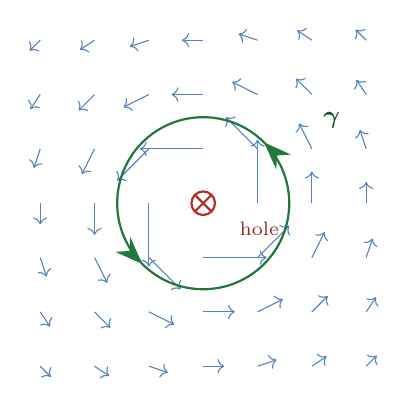
\begin{tikzpicture}[scale=1.15]
% vector field (-y,x)/(x^2+y^2) at grid points, skipping origin
\foreach \x in {-1.8,-1.2,-0.6,0,0.6,1.2,1.8}
  \foreach \y in {-1.8,-1.2,-0.6,0,0.6,1.2,1.8}
    {\pgfmathsetmacro{\rsq}{\x*\x+\y*\y}
     \pgfmathparse{\rsq > 0.1 ? 1 : 0}
     \ifnum\pgfmathresult>0
       \pgfmathsetmacro{\vx}{-0.42*\y/\rsq}
       \pgfmathsetmacro{\vy}{0.42*\x/\rsq}
       \draw[->, figB!75, thin] (\x,\y) -- ({\x+\vx},{\y+\vy});
     \fi}
% the hole at origin
\draw[figR, thick] (0,0) circle (0.13);
\draw[figR, thick] (-0.093,-0.093) -- (0.093,0.093);
\draw[figR, thick] (-0.093,0.093) -- (0.093,-0.093);
% unit circle path with orientation
\draw[thick, figG,
  postaction={decorate},
  decoration={markings,
    mark=at position 0.125 with {\arrow[figG, scale=1.5]{Stealth}},
    mark=at position 0.625 with {\arrow[figG, scale=1.5]{Stealth}}}]
  (0,0) circle (0.95);
\node[figG!70!black, font=\small] at (1.42,0.92) {$\boldsymbol{\gamma}$};
\node[figR!85!black, font=\scriptsize] at (0.62,-0.28) {hole};
\end{tikzpicture}%
\figcap{The vector field of $\omega = \frac{-y\,dx + x\,dy}{x^2+y^2}$ circulates around the removed origin. Locally the field is a gradient (the curl vanishes), but no global potential exists: the circle $\boldsymbol{\gamma}$ picks up $\int_{\boldsymbol{\gamma}}\omega = 2\pi$ per loop around the hole. The form measures the winding --- an analytic object detecting a topological feature.}
\end{center}

\begin{proposition}[Poincar\'{e} Lemma]
On a star-shaped domain $D \subseteq \R^n$ (i.e., there exists a point $\mathbf{p}_0 \in D$ such that the line segment from $\mathbf{p}_0$ to any $\mathbf{p} \in D$ lies entirely in $D$), every closed form is exact: $d\omega = 0 \;\Rightarrow\; \omega = d\eta$ for some $\eta$.

In particular, since $\R^n$ itself is star-shaped, every closed form on $\R^n$ is exact.
\end{proposition}

The proof (constructing $\eta$ explicitly via a homotopy operator) is beyond the scope of this course; see Lee, Chapter 17. The key point is that the failure of exactness is a \textit{topological} property of the domain --- it detects holes.

\subsection*{From Obstructions to Topology}

The space of closed forms modulo exact forms:
\[
H^k = \frac{\{\text{closed } k\text{-forms}\}}{\{\text{exact } k\text{-forms}\}}
\]

is called the \textbf{$k$-th de Rham cohomology group}. It measures the ``$k$-dimensional holes'' in the domain:
\begin{itemize}
    \item $H^0$ counts the connected components (a closed 0-form is a locally constant function; it is exact --- i.e., globally constant --- if and only if the domain is connected).
    \item $H^1$ detects 1-dimensional holes: loops that cannot be contracted to a point. The example above shows $H^1(\R^2 \setminus \{0\}) \neq 0$.
    \item $H^2$ detects 2-dimensional holes: closed surfaces that do not bound a volume.
\end{itemize}

This is the bridge from calculus to topology: the exterior derivative $d$, defined purely by differentiation, detects the \textit{shape} of the domain. This is the content of Chapters 17--18 of Lee's textbook (the 591 syllabus), and connects directly to the fundamental group $\pi_1$ from 590.

\subsection{Applications to Physics}

In physics, the exterior derivative on higher forms is not abstract at all --- it describes the fundamental forces.

The electromagnetic potential $A$ is a 1-form. Its exterior derivative $F = dA$ is a 2-form --- the electromagnetic field tensor (with 6 independent components: 3 for $\mathbf{E}$, 3 for $\mathbf{B}$, as discussed in \S21.3). Two of Maxwell's equations become:
\[
dF = 0 \qquad \text{(no magnetic monopoles; Faraday's law)}.
\]

This is just $d^2A = 0$ --- the identity $d^2 = 0$ is the reason magnetic monopoles do not exist (in classical electromagnetism). The other two Maxwell equations are $d{*}F = J$, where $*$ is the Hodge star and $J$ is the current 3-form.

More generally, in gauge theory and general relativity, the curvature of a connection is a 2-form, and the equations of motion (Yang--Mills, Einstein) are expressed as conditions on this curvature 2-form and its exterior derivative. The machinery of forms and $d$ is not a reformulation of known physics --- it is the \textit{native language} in which modern theoretical physics is written.

\section{The Generalized Stokes' Theorem}

\subsection{The Classical Theorems in Forms Language}

We now translate each of the four integral theorems from Parts I--II into the language of forms, showing explicitly that both sides become form integrals. The pattern that emerges will lead to the generalized theorem.

\subsubsection*{The Fundamental Theorem of Calculus}

Classical statement: $\int_a^b f'(x)\,dx = f(b) - f(a)$.

\textbf{Right-hand side.} Let $\omega = f$ be a 0-form. Its exterior derivative is $d\omega = df = f'(x)\,dx$ (a 1-form). So:
\[
\int_a^b f'(x)\,dx = \int_{[a,b]} d\omega.
\]

\textbf{Left-hand side.} The boundary of $[a,b]$ is the two-point set $\partial[a,b] = \{a, b\}$, with the induced orientation: $b$ gets $+$ (outward-pointing = rightward) and $a$ gets $-$ (outward-pointing = leftward). ``Integrating'' the 0-form $\omega = f$ over this oriented boundary means:
\[
\int_{\partial[a,b]} \omega = f(b) - f(a).
\]

\textbf{Result:}
\[
\int_{\partial[a,b]} \omega = \int_{[a,b]} d\omega. \quad \checkmark
\]

\subsubsection*{Green's Theorem}

Classical statement: $\oint_{\partial D} P\,dx + Q\,dy = \iint_D (Q_x - P_y)\,dx\,dy$.

\textbf{Right-hand side.} Let $\omega = f_1\,dx + f_2\,dy$ be a 1-form on $\R^2$ (with $f_1 = P$, $f_2 = Q$). Its exterior derivative is:
\[
d\omega = \big((f_2)_x - (f_1)_y\big)\,dx \wedge dy.
\]
This is a 2-form, and integrating it over $D$ gives:
\[
\iint_D d\omega = \iint_D \big((f_2)_x - (f_1)_y\big)\,dx\,dy.
\]

\textbf{Left-hand side.} Parametrize the boundary $\partial D = \boldsymbol{\gamma}(t) = (x(t), y(t))$ counterclockwise. Pull back the 1-form:
\[
\omega = f_1\,dx + f_2\,dy \quad \xrightarrow{\text{pullback}} \quad (f_1\,x' + f_2\,y')\,dt.
\]
So $\int_{\partial D} \omega = \int_a^b (f_1\,x' + f_2\,y')\,dt = \oint_{\partial D} f_1\,dx + f_2\,dy$.

\textbf{Result:}
\[
\int_{\partial D} \omega = \iint_D d\omega. \quad \checkmark
\]

\subsubsection*{Stokes' Theorem in $\R^3$}

Classical statement: $\iint_S (\nabla \times \mathbf{F}) \cdot \hat{n}\,dS = \oint_{\partial S} \mathbf{F} \cdot d\mathbf{r}$.

\textbf{Right-hand side.} Let $\omega = f_1\,dx + f_2\,dy + f_3\,dz$ be a 1-form (with $\mathbf{F} = (f_1, f_2, f_3)$). By the curl proposition (\S22.2):
\[
d\omega = \big((f_3)_y - (f_2)_z\big)\,dy \wedge dz + \big((f_1)_z - (f_3)_x\big)\,dz \wedge dx + \big((f_2)_x - (f_1)_y\big)\,dx \wedge dy.
\]
Now integrate over the surface $S$ parametrized by $\mathbf{X}(u,v)$. Each 2-form pulls back via the pullback proposition (\S22.1):
\begin{align*}
\iint_S d\omega &= \iint_D \big[(f_3)_y - (f_2)_z\big](y_u z_v - z_u y_v) + \big[(f_1)_z - (f_3)_x\big](z_u x_v - x_u z_v) \\
&\qquad + \big[(f_2)_x - (f_1)_y\big](x_u y_v - y_u x_v) \; du\,dv \\
&= \iint_D (\nabla \times \mathbf{F}) \cdot (\mathbf{X}_u \times \mathbf{X}_v)\,du\,dv.
\end{align*}

Now compare with the classical form: $\iint_S (\nabla \times \mathbf{F}) \cdot \hat{n}\,dS$. Since $\hat{n}\,dS = \frac{\mathbf{X}_u \times \mathbf{X}_v}{|\mathbf{X}_u \times \mathbf{X}_v|} \cdot |\mathbf{X}_u \times \mathbf{X}_v|\,du\,dv$, the norms \textbf{cancel}:
\[
\iint_S (\nabla \times \mathbf{F}) \cdot \hat{n}\,dS = \iint_D (\nabla \times \mathbf{F}) \cdot (\mathbf{X}_u \times \mathbf{X}_v)\,du\,dv = \iint_S d\omega.
\]

This cancellation is the key simplification: the forms framework never introduces $|\mathbf{X}_u \times \mathbf{X}_v|$ in the first place --- it works directly with the signed cross product components, which are the 2-form pullbacks.

\textbf{Left-hand side.} Parametrize the boundary $\partial S = \boldsymbol{\gamma}(t) = (x(t), y(t), z(t))$. Pull back:
\[
\omega = f_1\,dx + f_2\,dy + f_3\,dz \quad \xrightarrow{\text{pullback}} \quad (f_1\,x' + f_2\,y' + f_3\,z')\,dt = \mathbf{F} \cdot \boldsymbol{\gamma}'(t)\,dt.
\]
So $\int_{\partial S} \omega = \oint_{\partial S} \mathbf{F} \cdot d\mathbf{r}$.

\textbf{Result:}
\[
\int_{\partial S} \omega = \iint_S d\omega. \quad \checkmark
\]

\subsubsection*{The Divergence Theorem}

Classical statement: $\iint_{\partial V} \mathbf{F} \cdot \hat{n}\,dS = \iiint_V \nabla \cdot \mathbf{F}\,dV$.

\textbf{Right-hand side.} Let $\eta = f_{23}\,dy \wedge dz + f_{31}\,dz \wedge dx + f_{12}\,dx \wedge dy$ be a 2-form (with $\mathbf{F} = (f_{23}, f_{31}, f_{12})$). By the divergence proposition (\S22.2):
\[
d\eta = \big((f_{23})_x + (f_{31})_y + (f_{12})_z\big)\,dx \wedge dy \wedge dz = (\nabla \cdot \mathbf{F})\,dx \wedge dy \wedge dz.
\]
Integrating over $V$:
\[
\iiint_V d\eta = \iiint_V \nabla \cdot \mathbf{F}\,dV.
\]

\textbf{Left-hand side.} The boundary $\partial V$ is a closed surface. Parametrize each piece by $\mathbf{X}(u,v)$. The 2-form $\eta$ pulls back via \S22.1:
\begin{align*}
\iint_{\partial V} \eta &= \iint_D \big[f_{23}(y_u z_v - z_u y_v) + f_{31}(z_u x_v - x_u z_v) + f_{12}(x_u y_v - y_u x_v)\big]\,du\,dv \\
&= \iint_D \mathbf{F} \cdot (\mathbf{X}_u \times \mathbf{X}_v)\,du\,dv.
\end{align*}

Again the norm cancellation: since $\hat{n}\,dS = (\mathbf{X}_u \times \mathbf{X}_v)\,du\,dv$:
\[
\iint_{\partial V} \mathbf{F} \cdot \hat{n}\,dS = \iint_{\partial V} \eta.
\]

\textbf{Result:}
\[
\iint_{\partial V} \eta = \iiint_V d\eta. \quad \checkmark
\]

\subsection{Statement}

All four classical theorems have the same form: $\int_{\partial \Omega} \omega = \int_\Omega d\omega$, where $\omega$ is a form of one degree lower than the dimension of $\Omega$. This is the generalized Stokes' theorem.

\begin{theorem}[Generalized Stokes' Theorem]
Let $\Omega$ be an oriented, compact, piecewise smooth $k$-dimensional region with piecewise smooth boundary $\partial \Omega$ (with the induced orientation). If $\omega$ is a $(k-1)$-form that is $C^1$ on a neighborhood of $\Omega$, then:
\[
\boxed{\int_{\partial \Omega} \omega = \int_\Omega d\omega}
\]
\end{theorem}

\textbf{Reading the formula:} $\omega$ is one degree lower than the dimension of $\Omega$, so $\omega$ can be integrated over $\partial \Omega$ (which has dimension $k-1$), and $d\omega$ can be integrated over $\Omega$ (which has dimension $k$). The four classical theorems are this single identity applied at $k = 1, 2, 2, 3$:

\begin{center}
\renewcommand{\arraystretch}{1.5}
\begin{tabular}{|c|c|c|c|c|}
\hline
\textbf{$k$} & \textbf{$\Omega$} & \textbf{$\omega$} & \textbf{$d\omega$} & \textbf{Classical name} \\
\hline
1 & interval $[a,b]$ & 0-form $f$ & $f'\,dx$ & FTC \\
\hline
2 & region $D \subseteq \R^2$ & 1-form on $\R^2$ & curl $\cdot\,dx \wedge dy$ & Green's \\
\hline
2 & surface $S \subseteq \R^3$ & 1-form on $\R^3$ & curl $\cdot$ 2-form & Stokes' \\
\hline
3 & volume $V \subseteq \R^3$ & 2-form & div $\cdot\,dx \wedge dy \wedge dz$ & Divergence \\
\hline
\end{tabular}
\end{center}

\begin{center}
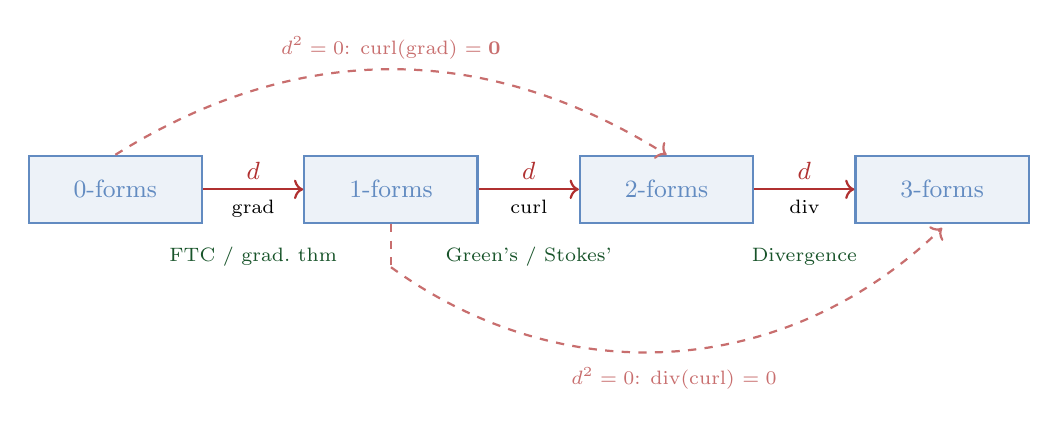
\begin{tikzpicture}[scale=1.0, every node/.style={font=\small}]
% ladder boxes
\node[draw, thick, figB!70, fill=figB!8, minimum width=2.2cm, minimum height=0.85cm] (f0) at (0,0) {0-forms};
\node[draw, thick, figB!70, fill=figB!8, minimum width=2.2cm, minimum height=0.85cm] (f1) at (3.5,0) {1-forms};
\node[draw, thick, figB!70, fill=figB!8, minimum width=2.2cm, minimum height=0.85cm] (f2) at (7,0) {2-forms};
\node[draw, thick, figB!70, fill=figB!8, minimum width=2.2cm, minimum height=0.85cm] (f3) at (10.5,0) {3-forms};
% d arrows
\draw[->, thick, figR] (f0) -- (f1) node[midway, above] {$d$} node[midway, below, font=\scriptsize, black] {grad};
\draw[->, thick, figR] (f1) -- (f2) node[midway, above] {$d$} node[midway, below, font=\scriptsize, black] {curl};
\draw[->, thick, figR] (f2) -- (f3) node[midway, above] {$d$} node[midway, below, font=\scriptsize, black] {div};
% theorem labels under the arrows
\node[figG!70!black, font=\scriptsize, align=center] at (1.75,-0.85) {FTC / grad.\ thm};
\node[figG!70!black, font=\scriptsize, align=center] at (5.25,-0.85) {Green's / Stokes'};
\node[figG!70!black, font=\scriptsize, align=center] at (8.75,-0.85) {Divergence};
% d^2 = 0 arcs
\draw[->, thick, dashed, figR!70] (f0.north) to[bend left=32] node[midway, above, font=\scriptsize] {$d^2 = 0$: curl(grad) $= \mathbf{0}$} (f2.north);
\draw[->, thick, dashed, figR!70] ($(f1.south)+(0,-0.55)$) to[bend right=40] node[pos=0.5, below=2pt, font=\scriptsize] {$d^2 = 0$: div(curl) $= 0$} ($(f3.south)+(0,-0.05)$);
\draw[dashed, figR!70, thin] (f1.south) -- ($(f1.south)+(0,-0.55)$);
\end{tikzpicture}%
\figcap{The ladder of forms in $\R^3$. Each rung of $d$ is one classical differential operator; each integral theorem trades one application of $d$ for one boundary operation $\partial$. The dashed arcs are the two vanishing identities --- both instances of $d^2 = 0$.}
\end{center}

\begin{remark}[The Punchline]
All four theorems are the same theorem:
\[
\int_{\partial \Omega} \omega = \int_\Omega d\omega.
\]

The apparent differences --- gradient vs curl vs divergence, line integrals vs surface integrals vs volume integrals --- arise from the same operation $d$ applied to forms of different degrees, integrated over regions of different dimensions.

The three identities $d^2 = 0$ ($\text{curl}(\text{grad}) = 0$, $\text{div}(\text{curl}) = 0$) are also a single identity. And the orientation signs that caused so much bookkeeping (the bottom surface normal, the boundary curve direction, the $f(b) - f(a)$ sign) are all automatically handled by the wedge product's anti-commutativity.

This is why differential forms are the natural language for integration on manifolds: a single theorem, a single derivative, a single product rule for signs.
\end{remark}

\end{document}
